\documentclass[
fontsize=10pt, % Base font size
twoside=true, % Use different layouts for even and odd pages (in particular, if twoside=true, the margin column will be always on the outside)
%open=any, % If twoside=true, uncomment this to force new chapters to start on any page, not only on right (odd) pages
%chapterprefix=true, % Uncomment to use the word "Chapter" before chapter numbers everywhere they appear
%chapterentrydots=true, % Uncomment to output dots from the chapter name to the page number in the table of contents
numbers=noenddot, % Comment to output dots after chapter numbers; the most common values for this option are: enddot, noenddot and auto (see the KOMAScript documentation for an in-depth explanation)
%draft=true, % If uncommented, rulers will be added in the header and footer
%overfullrule=true, % If uncommented, overly long lines will be marked by a black box; useful for correcting spacing problems
]{kaobook}

%%%% set to 1 to add 1st Author Publications in the manuscript
\def\addpublications{0}

%%%%%% Font and languages
\usepackage{palatino}

\usepackage[english]{babel} % Load characters and hyphenation
\usepackage[english=british]{csquotes}	% English quotes

%%%%%% to include pdf files (in the appendix)
%\usepackage{pdfpages}

%%%%%% section and subsection properties
\usepackage{titlesec}
\usepackage{sectsty}
% set section/subsections HEADINGS font and color
\definecolor{ColorSection}{rgb}{0.8,0.0,0.0} %mix personal color
\definecolor{ColorSubSection}{rgb}{0.2,0.4,0.6} %mix personal color
\sectionfont{\color{ColorSection}}  % sets colour of sections
\subsectionfont{\color{ColorSubSection}}  % sets colour of subsections

%%%%%% numerote aussi les subsections
\setcounter{secnumdepth}{3}

%%%%%% enlarge the default width of the dictum (0.333 default)
\renewcommand{\dictumwidth}{0.7\textwidth}

%%%%%% epigraph (inspirational quote at the beginning of a chapter)
\usepackage{epigraph}

%%%%%% Table
\usepackage{tabularx} % smarter arrays

%%%%%% Maths
\usepackage{physics}

\DeclareMathSymbol{\Omega}{\mathalpha}{letters}{"0A}% italics
\DeclareMathSymbol{\varOmega}{\mathalpha}{operators}{"0A}% upright
\providecommand*{\upOmega}{\varOmega}% for siunitx
\usepackage{siunitx}
% Note that the sign must be
%  µ
%  MICRO SIGN
%  Unicode: U+00B5, UTF-8: C2 B5
% and \emph{not}
%  μ
%  GREEK SMALL LETTER MU
%  Unicode: U+03BC, UTF-8: CE BC
\sisetup{math-micro=\text{µ},text-micro=µ}


%%%%%% definitions of mathematical variables
\newcommand{\abf}{{\mathbf a}}
\newcommand{\bbf}{{\mathbf b}}
\newcommand{\ebf}{{\mathbf e}}
\newcommand{\hbf}{{\mathbf h}}
\newcommand{\jbf}{{\mathbf j}}
\newcommand{\kbf}{{\mathbf k}}
\newcommand{\rbf}{{\mathbf r}}
\newcommand{\nbf}{{\mathbf n}}
\newcommand{\ubf}{{\mathbf u}}
\newcommand{\vbf}{{\mathbf v}}
\newcommand{\xbf}{{\mathbf x}}
\newcommand{\Abf}{{\mathbf A}}
\newcommand{\Bbf}{{\mathbf B}}
\newcommand{\Hbf}{{\mathbf H}}
\newcommand{\Jbf}{{\mathbf J}}
\newcommand{\Dbf}{{\mathbf D}}
\newcommand{\Ebf}{{\mathbf E}}
\newcommand{\Kbf}{{\mathbf K}}
\newcommand{\Mbf}{{\mathbf M}}
\newcommand{\Sbf}{{\mathbf S}}
\newcommand{\Vbf}{{\mathbf V}}
\newcommand{\Sbb}{{\mathbb S}}
\newcommand{\nablabf}{\mbox{\boldmath${\nabla}$}}
\newcommand{\diff}{{\mathrm{d}}}
\newcommand{\SWR}{{\mathrm{SWR}}}
\newcommand{\Vfwd}{{v_{\mathrm{f}}}}
\newcommand{\Ifwd}{{i_{\mathrm{f}}}}
\newcommand{\Vrefl}{{v_{\mathrm{r}}}}
\newcommand{\Irefl}{{i_{\mathrm{r}}}}
\newcommand{\Vbff}{{\mathbf{V}_{\mathrm{f}}}}
\newcommand{\Vbfr}{{\mathbf{V}_{\mathrm{r}}}}
\newcommand{\Zref}{{Z_{\mathrm{ref}}}}

\newcommand{\TE}{{\mathrm{TE}}}
\newcommand{\TM}{{\mathrm{TM}}}

\newcommand{\degC}{$\si{\degreeCelsius}$ }
%%%%%% Bibliography
% Load the bibliography package and pass it some options
\usepackage[sorting=none,
			sortcites=true,
			citestyle=numeric-comp,
			bibstyle=authoryear]{styles/kaobiblio}
% Bibliography files
\addbibresource{references.bib}

% Use the "none" sorting for the document
\assignrefcontextentries[]{*}

% Redefine the citation style to Author (year) and using bracket like [i-ii]
\RenewDocumentCommand{\formatmargincitation}{m}{
	\parencite{#1} \citeauthor*{#1} (\citeyear{#1})\\
}

%%%% General TOC depth
\setcounter{tocdepth}{3}

%%%% Margin TOC depth
\renewcommand{\themargintocdepth}{1}



% Redefine the citation style: uses numbered sidenotes (upperscript)
%\RenewDocumentCommand{\formatmargincitation}{m}{%
%	\supercite{#1} \citeauthor*{#1} (\citeyear{#1})\\
%}
%
% redefine sidecite to use upperscript numbers
%\RenewDocumentCommand{\sidecite}{m}{%
%	\supercite{#1}%
%	\margincitation{#1}%
%}

% Citing author and date in the text 
\NewDocumentCommand{\citeauthyear}{m}{%
	\citeauthor*{#1} (\citeyear{#1})
}

%\makeindex[columns=3, title=Alphabetical Index, intoc] % Make LaTeX produce the files required to compile the index

%\makeglossaries % Make LaTeX produce the files required to compile the glossary

%\makenomenclature % Make LaTeX produce the files required to compile the nomenclature

% fix bad unicode character which may arise from copy/paste
\DeclareUnicodeCharacter{202F}{\,}

% ###### listing stuff
\definecolor{codegreen}{rgb}{0,0.6,0}
\definecolor{codegray}{rgb}{0.5,0.5,0.5}
\definecolor{codepurple}{rgb}{0.58,0,0.82}
\definecolor{backcolour}{rgb}{0.95,0.95,0.92}

\lstdefinestyle{mystyle}{
	backgroundcolor=\color{backcolour},  
	commentstyle=\color{codegreen},
	keywordstyle=\color{magenta},
	numberstyle=\tiny\color{codegray},
	stringstyle=\color{codepurple},
	basicstyle=\footnotesize,
	breakatwhitespace=false,        
	breaklines=true,                
	captionpos=b,                   
	keepspaces=true,                
	numbers=left,                   
	numbersep=5pt,                 
	showspaces=false,               
	showstringspaces=false,
	showtabs=false,                 
	tabsize=2
}

\lstset{style=mystyle}

%----------------------------------------------------------------------------------------
\begin{document}
	
	%----------------------------------------------------------------------------------------
	%	TITLE
	%----------------------------------------------------------------------------------------
	
	%\titlehead{The \texttt{kaobook} class}
	\subject{Habilitation à Diriger les Recherches}
	
	\title[HDR]{Enhancing Performances of High Power Radio-Frequency
		Systems in Magnetic Confinement Fusion Devices}
	%\subtitle{Customise this page according to your needs}
	
	\author[Julien Hillairet]{Julien Hillairet}
	
	\date{\today}
	
	%\publishers{An Awesome Publisher}
	
	%----------------------------------------------------------------------------------------
	
	\frontmatter % Denotes the start of the pre-document content, uses roman numerals
	
	%----------------------------------------------------------------------------------------
	%	OPENING PAGE
	%----------------------------------------------------------------------------------------
	
	%\makeatletter
	%\extratitle{
	%	% In the title page, the title is vspaced by 9.5\baselineskip
	%	\vspace*{9\baselineskip}
	%	\vspace*{\parskip}
	%	\begin{center}
	%		% In the title page, \huge is set after the komafont for title
	%		\usekomafont{title}\huge\@title
	%	\end{center}
	%}
	%\makeatother
	
	
	%----------------------------------------------------------------------------------------
	%	DEDICATION
	%----------------------------------------------------------------------------------------
	
	\dedication{
		\begin{center}
			\includegraphics[width=1\linewidth]{figures/electromagnetic_spectrum_small}
		\end{center}
		\flushright -- Randall Munroe, \href{https://xkcd.com/273/}{XKCD\#273}
	}
	
	%----------------------------------------------------------------------------------------
	%	OUTPUT TITLE PAGE AND PREVIOUS
	%----------------------------------------------------------------------------------------
	
	% Note that \maketitle outputs the pages before here
	
	% If twoside=false, \uppertitleback and \lowertitleback are not printed
	% To overcome this issue, we set twoside=semi just before printing the title pages, and set it back to false just after the title pages
	\KOMAoptions{twoside=semi}
	\maketitle
	\KOMAoptions{twoside=false}
	
	%----------------------------------------------------------------------------------------
	%	RESUME
	%----------------------------------------------------------------------------------------
	%\pagelayout{wide} % No margins
	%	\addpart{intro}
	% French Summary
	\chapter*{Résumé}
\selectlanguage{french}

La fusion est le processus nucléaire qui fait briller le soleil comme toutes les étoiles de l'univers et que l'on cherche à maîtriser sur terre. À l’opposé de la fission nucléaire, la fusion consiste à créer un noyau atomique plus lourd à partir de plusieurs noyaux légers. Sur Terre, la maîtrise de la fusion présenterait beaucoup d’avantages en comparaison de la fission nucléaire, en termes de densité énergétique, de sécurité, de ressources en combustibles et sans production intrinsèque de gaz à effet de serre. 

Toutefois, reproduire les conditions de température favorables à la fusion, soit entre 100 et 200 millions de degrés Celsius (10-20 keV) n’est pas trivial. À ces températures, la matière se présente sous forme de plasma : les électrons composant les noyaux atomiques ont été arrachés, générant ainsi un mélange d’ions et d’électrons qui ne sont plus liés entre eux. Ce plasma peut être confiné et contrôlé en lui imposant un puissant champ magnétique : c’est ce qu’on réalise dans des machines de recherche appelées tokamaks, par exemple le tokamak WEST (anciennement Tore Supra) situé sur le centre CEA de Cadarache dans les Bouches-du-Rhône. Bien que les performances obtenues sur les différentes installations dans le monde aient continuellement progressées depuis plus de 50 ans, le rendement énergétique défini par le rapport entre l'énergie libérée par la fusion et l'énergie injectée dans le plasma pour obtenir les conditions de fusion reste encore inférieur à 1. Le projet international Iter, en cours de construction à Cadarache, doit démontrer qu'il est possible d'obtenir un rapport de 5 à 10.

Afin d'obtenir des températures de plusieurs dizaines de millions de degrés, des systèmes radiofréquences sont utilisés couramment sur différentes installations expérimentales dans le monde. Ces systèmes vont générer puis transmettre jusqu'au plasma des ondes électromagnétiques dont la puissance est de l'ordre de plusieurs mégawatts. Selon leurs fréquences (de plusieurs MHz à une centaine de GHz), elles vont transférer leur énergie de préférence aux ions ou aux électrons du plasma, voire générer du courant électrique dans le plasma, afin d'augmenter la durée de maintien du plasma. Dans un tokamak, ces ondes sont injectées dans le plasma par des antennes situées à proximité de ce dernier. Ces antennes doivent être conçues pour opérer sous vide à des tensions et courants de plusieurs dizaines de kilovolts at kiloampères, sur des temps longs, tout en supportant les divers flux thermiques et de particules en provenance du plasma. Ces conditions sévères, voire hostiles, sont exclusives à ces machines de recherche et par conséquent la littérature scientifique sur ce sujet est peu abondante.

Ce manuscrit décrit une partie de mon travail réalisé au CEA/IRFM depuis 2008 en tant qu'ingénieur radio-fréquence et physicien des plasmas sur la conception de ces antennes ou de leurs éléments ainsi que de l'analyse de leurs intéractions avec le plasma. 

Les deux premiers chapitres sont des introductions et des rappels théoriques nécessaires à la lecture des chapitres suivants. Le chapitre 1 est une introduction à la fusion nucléaire contrôlée et aux systèmes de chauffage et de génération de courant pour des plasmas de tokamaks. Les principaux éléments composants les systèmes radio-fréquences utilisés pour le chauffage et la génération de courant dans les plasmas de tokamak sont également décrits dans ce chapitre. Le chapitre 2 rappelle les éléments théoriques permettant la description de la propagation des ondes électromagnétiques dans les lignes de transmission jusqu'au plasma faisant face aux antennes.

Le chapitre 3 décrit mes travaux concernant le couplage des ondes radio-fréquence excitées par les antennes au plasma de tokamaks. Ce chapitre débute par une rapide introduction théorique aux ondes dans les plasmas, en particulier aux domaines de fréquences dits Cyclotronique Ioniques et Hybride Basse qui concerne ce manuscrit. Le couplage de ces ondes au plasma est analysé de deux façons pour les ondes Hybrides Basses : i) grâce à une formulation semi-analytique implémentée dans le code ALOHA ou ii) en utilisant des codes de calcul commerciaux. Les résultats numériques obtenus sont comparés avec  des expériences réalisées sur le tokamak Tore Supra.

Les chapitre 4 et 5 portent sur plusieurs exemples de travaux relatifs à la conception d'antennes radio-fréquences ou de leurs éléments. Le chapitre 4 est dédié à la gamme de fréquence Cyclotronique Ionique (dizaines de MHz). La première partie détaille les travaux réalisés à partir de 2013 concernant la conception des antennes Cyclotroniques Ioniques pour le tokamak WEST. La seconde partie de ce chapitre est consacrée aux travaux réalisés et encadrés dans le cadre de la R\&D menée sur les contacts électriques glissants pour le système Cyclotronique Ionique d'ITER. Le chapitre 5 est quant à lui consacré aux activités de conceptions et de tests de composants radiofréquences pour le système à la fréquence Hybride Basse d'ITER, réalisés entre 2010 et 2014.

Le chapitre 6 rapporte les travaux d'étudiants encadrés sur la thématique des arcs et notamment du phénomène multipactor. Ces travaux ont été menés en collaboration avec le CNES et l'ONERA.

Enfin, le chapitre 7 porte sur mes activités d'enseignement et de vulgarisation réalisés au CEA/IRFM, pour des tranches d'âges diverses allant du collège jusqu'aux étudiants de Master 2. Ce chapitre se termine par la description de mon activité autour du logiciel libre, en particulier le développement du package Python scikit-rf.



\selectlanguage{english}


	
	% English Summary
	\setchapterstyle{kao}
%\setchapterpreamble[u]{\margintoc}
\chapter*{Summary}
%\labch{intro}

Magnetic confinement is currently the most advanced technique to master nuclear fusion for energy production. One of the main requirements for achieving fusion is to heat the plasma particles to temperatures exceeding 100-200 million of degrees (10-20 keV). Electromagnetic waves in mega-watt range of power, from tens of MHz to hundreds of GHz, are launched by antennas located near the plasma periphery in order to increase the plasma temperature and extend its duration. However, designing and using multi-megawatts RF systems is not trivial and leads to many issues, which for some of them  are relatively little addressed in the literature. 

This manuscript describes part of my work performed at CEA/IRFM since 2008 as RF research scientist in order to enhance the performances of high-power RF systems for magnetic confinement fusion devices. It is organized as follows. 

The Chapter \ref{chap:fusion_and_rf} is an introduction to the controlled nuclear fusion and explain the need for Heating and Current Drive systems in Tokamaks. The main elements of the RF systems used in current experimental devices are identified in this chapter. Fusion scientists can easily skip this chapter. 

The Chapter \ref{chap:RF_fundamentals} recalls the theoretical elements of the electromagnetic theory which are necessary for the daily work of a RF engineer working in RF Heating and Current Drive systems for tokamaks. This chapter is not intended to teach specialists in the RF field anything, but just to bring together in one place the essential RF quantities and figures or merit. 

The Chapter \ref{chap:rf_coupling} describes my work on the coupling of RF waves from antennas to tokamak plasmas. After in introduction to waves in plasma, in particular in the Ion Cyclotron and Lower Hybrid range of frequencies, we describe the Lower Hybrid Range of Frequency (LHRF) coupling code ALOHA and some examples of its use on Tore Supra experiments. The last part of this chapter is dedicated to the use of full-wave software for the coupling calculations.

The Chapters \ref{chap:ICRF} and \ref{chap:LHRF} describe my work for the design and tests of high power devices for RF heating and current drive in tokamaks. Chapter 4 is dedicated to Ion Cyclotron Range of Frequency (ICRF). It concerns my work on the WEST ICRF antennas design and modelling which has started in 2013. Another important topic of this chapter concerns the R\&D performed on the ITER ICRF system, specifically on RF contacts. The Chapter 5 addresses the design and tests of RF devices for the LHRF from 2010 to 2014, which concerns in particular components for the then foreseen ITER LHCD system.

The Chapter \ref{chap:Multipactor} introduces the research carried out on topic of RF breakdowns and in particular the multipactor effect. This work has been made in collaboration with CNES and ONERA since 2014.

Finally, the Chapter \ref{chap:Fusion Education} describes parallel teaching and outreaching activities performed at CEA/IRFM, on the topic of the "Fusion Education". This chapter also addresses my work on open-source software developments, in particular on the Python package \href{http://scikit-rf.org/}{scikit-rf}. 

%This manuscript does not cover some of my work at CEA/IRFM performed since 2008, such as on RF plasma cleaning in the frame of the ITER Wide-Angle Visible (WAVS) diagnostic or my work as WEST Engineer-in-Charge (the \href{https://github.com/IRFM/PPPAT/}{PPPAT software}), neither a rapid excursion in the Electron Cyclotron world in (\citeauthyear{farthouat2010}).

	
	%\pagelayout{margin} % Restore margins
	
	%----------------------------------------------------------------------------------------
	%	TABLE OF CONTENTS & LIST OF FIGURES/TABLES
	%----------------------------------------------------------------------------------------
	
	\begingroup % Local scope for the following commands
	
	% Define the style for the TOC, LOF, and LOT
	%\setstretch{1} % Uncomment to modify line spacing in the ToC
	%\hypersetup{linkcolor=blue} % Uncomment to set the colour of links in the ToC
	\setlength{\textheight}{23cm} % Manually adjust the height of the ToC pages
	
	% Turn on compatibility mode for the etoc package
	\etocstandarddisplaystyle % "toc display" as if etoc was not loaded
	\etocstandardlines % "toc lines as if etoc was not loaded
	
	\tableofcontents % Output the table of contents
	
	%\listoffigures % Output the list of figures
	
	% Comment both of the following lines to have the LOF and the LOT on different pages
	%\let\cleardoublepage\bigskip
	%\let\clearpage\bigskip
	
	%\listoftables % Output the list of tables
	
	\endgroup
	
	%----------------------------------------------------------------------------------------
	%	MAIN BODY
	%----------------------------------------------------------------------------------------
	
	\mainmatter % Denotes the start of the main document content, resets page numbering and uses arabic numbers
	
	% Fusion and tokamak
	% controlled fusion and RF heating and current drive
\setchapterimage[3.3cm]{figures/chap1/chapter_head} % Optionally specify theheight
\setchapterpreamble[u]{\margintoc}
\chapter{Controlled Fusion, RF heating and Current Drive}
\label{chap:fusion_and_rf}


%%%%%%%%%%%%%%%%%%%%%%%%%%%%%%%%%%%%%%%%%%
%%%%%%%%%%%%%%%%%%%%%%%%%%%%%%%%%%%%%%%%%%
\section{Nuclear Fusion}\label{sec:nuclear_fusion}
\subsection{Fusion Power}\label{sec:fusion_power}
\marginnote{Part of this section are taken from Master Fusion lecturer notes on Tokamak dimensioning, organized at CEA/IRFM for the French Fusion Master students in 2019 and 2020. This teaching work also led to the paper  \citeauthyear{sarazin2019}.}
\marginnote[+2.5cm]{Some figures in this manuscript, like Figures~\ref{fig:chap1:reactivity} and \ref{fig:chap1:nTtau_machines}, have been made in the frame on an \href{https://github.com/alfkoehn/fusion_plots/}{open-source project} created in collaboration with Alf Koehn from the University of Stuttgart, which purpose is to reproduce classic figures used in Fusion textbooks using open-source codes and data.}
Nuclear fusion is the process that powers all the stars in the Universe, including our Sun. If controlled in a reactor, fusion power could be an ideal energy source. It would run on hydrogen isotopes\sidenote[][+5cm]{Such as deuterium which can be found in sea water and tritium which can be generated inside the reactor}, does not generate greenhouse gas and creates no radioactive waste except the reactor vessel components itself. It would be a dispatchable source (in contrast to intermittency inherently affecting solar and wind energies) and would require much less land area than wind or solar power installations for similar power. But producing a self-sustaining fusion reaction requires that deuterium and tritium be heated to over 150~million~\si{K}, a temperature at which they become plasma: an electrically charged gas. 

Indeed, to get nuclear fusion, nuclei have to come close enough to each other where nuclear forces can overcome their mutual electrostatic repulsion. This would require temperatures of the order of 720 \si{keV} for head-on collisions of thermal particles to lead to fusion reactions in a classical way. 

Actually, quantum physics has to be taken into account in the process. Both in tokamaks and in stars interiors, fusion reactions take place predominantly due to the tunnel effect. Crossing this electrostatic barrier can be quantified in a probabilistic manner with the \textit{reaction rate} $r$ $[\si{reaction/(m^3.s)}]$, defined as the probability of reaction per unit time and volume. 
The reaction rate between mono-energetic ions "1" of density $n_1$ $[\si{m}^{-3}]$ striking target ions "2" of density $n_2$ $[\si{m}^{-3}]$ is proportional to the effective cross-section area $\sigma_{12}$ $[\si{m}^2]$ and to the velocity difference $v_{12}$ between the two species:
\begin{equation*}
	r_{12} = n_1 n_2 \; \sigma_{12} v_{12}
\end{equation*}
The quantity  $\sigma_{12} v_{12}$, which depends on the kinetic energy of the colliding particles, is called the \textit{reactivity} ($\mathrm{[m^3/s]}$). The reaction rate $r_{12}$ is proportional to the square of the density of the mixture. In fusion plasmas, ions are not mono-energetic, they are assumed to have Maxwellian velocity distributions. The average reactivity $\langle \sigma_{12} v \rangle_{12}$ derives from the following expression:
\begin{equation*}
	\left < \sigma v \right >_{12} 
	= \int_{-\infty}^{+\infty} \int_{-\infty}^{+\infty} 
	\sigma(v_{12}) v_{12}\;  f_1(v_1) f_2(v_2) \; dv_1dv_2
\end{equation*}

Finally, the average reaction rate $\left < r_{12} \right >$ reads:
\begin{equation*}
	\left < r_{12} \right > = n_1 n_2 \; \left < \sigma v \right >_{12}
\end{equation*}
The temperature dependence of the reactivity $\langle \sigma v \rangle_{12}$ is plotted on Figure~\ref{fig:chap1:reactivity} for several fusion reactions.

\begin{figure} 
	\begin{center}
		\includegraphics[width=1.0\textwidth]{figures/chap1/Fusion_Reactivity.png}
		\caption{Fusion reactivity versus temperature for few couples of fusion reactions. Data from \citeauthyear{richardson2019}.}
		\label{fig:chap1:reactivity}
	\end{center}
\end{figure}

From Figure~\ref{fig:chap1:reactivity}, the Deuterium (D)-Tritium (T) reactivity $\left<\sigma v\right>_{\mathrm{DT}}$ reaches its maximum for a temperature of 64 keV, corresponding to a temperature of $742\times10^6$ K. Since it has the highest reaction rate, the D-T reaction is the “easiest” to initiate (maximum reactivity at lowest temperature) of all fusion reactions and is the main targeted reaction for controlled fusion reactors\sidecite{cea1987, ball2019}: 
\begin{equation}
	\mathrm{D + T} \longrightarrow \mathrm{{}^4 He~(3.56~MeV) + n~(14.03~MeV)}
\end{equation}

The D-T reaction leads to a total released energy of $E_{DT}$ = 17.59~\si{MeV} = $2.82\times 10^{-12}$~\si{J} per fusion reaction, where almost 80\% of the energy is carried by the neutrons\sidenote{This value can be compared to the 200~MeV released by $^{235}$U fission. Yet, the energy release \emph{per nucleon} ($i.e.$ per kilogram) is approximately 4 times larger for fusion than for fission reactions.}. Assuming equal deuterium and tritium densities $n_D = n_T = \frac{n}{2}$, with $n$ the electron density, then the thermonuclear power density reads:

\begin{equation}
p_{\mathrm{DT}} = 
	\frac{n^2}{4}  \left< \sigma v \right>_{\mathrm{DT}} E_{\mathrm{DT}}
	\label{eq:fusion_power}
\end{equation}

The total fusion power $P_{\mathrm{fus}}=\int p_{\mathrm{DT}} \diff V$ is distributed among the alpha particles and the neutrons: 
\begin{equation}
P_{\mathrm{fus}}
= 
P_\alpha + P_n 
\doteq
\lambda \; P_\alpha
\label{eq:P_fus_Palpha}
\end{equation}
where we defined $\lambda = 17.59/3.56 \approx 4.94$ for a reason which will be clear in the next section.


%Assuming a constant reactivity in the plasma ("flat profile hypothesis") and using the tore volume $V$, the fusion power is: 
%\begin{equation}
%P_{fus} = \frac{V}{4}
%n^2 \left< \sigma v \right>_{DT} E_{DT}
%\end{equation}
%
%For a circular cross-section, the plasma volume is $V=2\pi^2 R a^2$. The reactivity $\left< \sigma v \right>_{DT}$ depends on the temperature. In the temperature range 10.3-18.5 keV, it turns out that the reactivity $\left< \sigma v \right>_{DT}$ can well (with about 10$\%$ error) be approximated by \sidecite{wesson2011}: 
%\begin{equation*}
%	\left< \sigma v \right>_{DT} \approx 1.18\, 10^{-24}\; \hat T^2 \;\si{\left[m^3 s^{-1}\right]}
%\end{equation*}
%where $\hat T$ is expressed in $\si{keV}$.

%%%%%%%%%%%%%%%%%%%%%%%%%%%%%%%%%%%%%%%%%%
\subsection{Triple Product}
At equilibrium in a fusion power plant, sources terms equal loss terms:
\begin{equation}
	\sum_{\mathrm{sources}} P = \sum_{\mathrm{loss}} P
	\label{eq:power_balance_general}
\end{equation}

Sustaining a high temperature plasma in a steady-state regime requires a plasma confinement method. In stars, the plasma is confined due to their gravitational field. Such kind of confinement is not applicable on Earth. Instead, the plasma can be trapped by strong magnetic field. In this manuscript, only magnetic confinement technique is discussed, which is the method used in tokamak, described in the next section. 

In magnetic confinement fusion reactors, while neutrons leave the plasma, charged nuclei, such as the Helium nucleus (also known as $\alpha$~particles) in the case of D-T reactions, are confined by a magnetic field and should ideally transfer their energy to the main ions before being extracted\footnote{There are basically 2 ways for this energy transfer. Since the collision frequency scales like the velocity difference between the colliding species to the power $-3$ ($\nu_{coll,ss'}\sim n_{s'}/\Delta v_{ss'}^3$), alpha particles transfer their energy dominantly to the electrons, which are much faster due to their low inertia. Then two routes are possible for the energy transfer from the electrons to the ions. Either via collisions, or via turbulence. The relative weight of those two channels is still a matter of research.}. The source term is the sum of alpha heating $P_\alpha$ and other plasma heating $P_{H}$ mechanisms:

\begin{equation}
\sum_{\mathrm{sources}} P
	\doteq 
	P_\alpha + P_{H} 
	\label{eq:sources}
\end{equation}

The losses origins being diverse, it is convenient to separate losses into thermal transport losses $P_{\mathrm{con}}$ (conduction and convection) and radiative losses $P_{\mathrm{rad}}$\sidecite{wesson2011}. Usually, the energy confinement time $\tau_E$ [\si{s}] is defined as the characteristic time at which the total thermal plasma energy $W=3 n k_B T$ is lost to its environment, either by collisional conduction or by turbulent thermal convection:

\begin{equation}
\sum_{\mathrm{loss}} P 
	=
	P_{\mathrm{con}} + P_{\mathrm{rad}}
	\doteq 
	\frac{ W }{ \tau_E } + P_{\mathrm{rad}}
	\label{eq:losses}
\end{equation}
Thus, at the equilibrium, power conservation leads to:
\begin{equation}
P_\alpha + P_{H} = \frac{ W }{ \tau_E } + P_{\mathrm{rad}}
\end{equation}
Keeping only conduction losses and ignoring radiation loss (which is a large approximation) and assuming the plasma is mainly heated by $\alpha$ particles ($P_H\ll P_\alpha$), Lawson\sidecite{lawson1957} estimated a criteria for which fusion power exceeds the losses, which leads to the following criteria (or "triple product"):
\begin{equation*}
	P_{\mathrm{fus}}/\lambda > \frac{3n k_B T}{\tau_E}
	\Rightarrow
	n \tau_E T > 
		\frac{12 \lambda k_B}{E_{\mathrm{DT}}} 
		\frac{T^2}{\left<\sigma v \right>_{\mathrm{DT}}}
\end{equation*}
As illustrated in Figure~\ref{fig:chap1:reactivity}, the reactivity $\left<\sigma v \right>_{\mathrm{DT}}$ depends on the temperature. The quantity $T_i^2 / \left<\sigma v \right>_{\mathrm{DT}}$ is found to have an absolute minimum around 14 $\si{keV}$. In this temperature region, the D-T reactivity can be approximated as $\left<\sigma v \right>_{\mathrm{DT}}\approx 1.1\times10^{-24} \hat{T}^2$~\sidecite{wesson2011,cea1987}. 
\marginnote[*+2]{$\hat T$ is expressed in \si{keV}: $\hat T=10^{-3} k_B T_{[K]}/e$}
This leads to:
\begin{equation}	
	n \hat{T} \tau_E > 3\times 10^{21} \, \si{keV.s.particles/m^3}
	\label{eq:lawson_criteria}
\end{equation}
Past or current fusion reactors achieved so far 1/10th of this value, but 30 years ago they only achieved 1/100 000th of it. Some of these performances are illustrated for various present and future magnetic confinement devices in Figure~\ref{fig:chap1:nTtau_machines}.



\begin{figure} 
	\begin{center}
		\includegraphics[width=1.0\textwidth]{figures/chap1/nTtau_machines.png}
		\caption{triple-product $n T_i \tau_E$ as a function of ion temperature $T_i$ for various devices (including stellarators, tokamaks, spherical tokamaks). Figure from \href{https://github.com/alfkoehn/fusion_plots/releases/tag/v1.0.0}{Alf Koehn}.}
		\label{fig:chap1:nTtau_machines}
	\end{center}
\end{figure}



% ####################################################
% ####################################################
% ####################################################
\section{Tokamak}
The magnetic device called \emph{tokamak}, first developed in the Soviet Union in the early 1960s, is an efficient way to confine high temperature plasmas\sidecite{shafranov2001, azizov2012, mirnov2019}. It is an axially symmetric field configuration with a large toroidal magnetic field, a moderate plasma pressure and a relatively small toroidal current\sidecite{Freidberg2007}. By virtue of the highest achieved values of the $n T \tau_e$ product, tokamak is presently the leading magnetic configuration for a fusion reactor. Because of its performance, there is a large number of experimental tokamaks currently in operation or being constructed\footnote{See \href{http://www.tokamak.info/}{www.tokamak.info} for an updated list of past, present and future experiments.}. The following machines are cited in this manuscript: WEST (previously Tore-Supra, Cadarache, France), JET (Culham, UK), ASDEX-Upgrade (Garching, Germany), EAST (Hefei, China), HL-2A (Chengdu, China), KSTAR (Deajon, Korea) and the international project ITER (Cadarache, France).

\begin{marginfigure}
	\includegraphics[width=1\linewidth]{figures/chap1/tokamak_toroidal_field}
	\caption{Toroidal magnetic field produced by toroidal field coils.}
	\label{fig:tokamak_toroidal_field}
\end{marginfigure}

\begin{marginfigure}
	\includegraphics[width=1\linewidth]{figures/chap1/tokamak_poloidal_field}
	\caption{Poloidal magnetic field produced by the plasma current.}
	\label{fig:tokamak_poloidal_field}
\end{marginfigure}

\begin{marginfigure}
	\includegraphics[width=1\linewidth]{figures/chap1/tokamak_helical_field}
	\caption{Helical magnetic field produced by the combination of toroidal and poloidal fields.}
	\label{fig:tokamak_helical_field}
\end{marginfigure}

In a tokamak, the plasma is confined by the combination of two magnetic fields: the toroidal and the poloidal fields. The toroidal field is the strongest one and is created in the toroidal direction by external "toroidal" field coils (Fig.\ref{fig:tokamak_toroidal_field}). Another set  of  external  coils, the poloidal field coils, which includes the central solenoid coils and additional control coils, are located concentric with the toroidal vacuum vessel.

An electric field in the toroidal direction is induced through the plasma by ramping a current in the central solenoid, like an electrical transformer in which the plasma acts as the secondary winding. This electric field induces a current in the plasma, which creates the poloidal field (Fig.\ref{fig:tokamak_poloidal_field}). Poloidal and toroidal magnetic fields add up to form a twisted helical field (Fig.\ref{fig:tokamak_helical_field}) and both are required to confine the plasma into the vacuum vessel. 

As seen in Section~\ref{sec:fusion_power}, achieving optimum reaction rates requires reaching temperatures above few tens of \si{keV} and hence to heat the confined plasma.


%%%%%%%%%%%%%%%%%%%%%%%%%%%%%%%%%%%%%%%%%%
%%%%%%%%%%%%%%%%%%%%%%%%%%%%%%%%%%%%%%%%%%
\subsection{Ohmic Heating}
The plasma current density $J_p$ $[\si{A/m^2}]$ flowing through plasma with resistivity $\eta$ $[\si{\Omega.m}]$ heats up the plasma and generates an Ohmic heating power density $p_\Omega$:

\begin{equation}\label{eq:ohmic_power_density}
p_\Omega = \eta \; J_p^2 \;\; \si{[W/m^3]}
\end{equation}

where $\eta$ is the classical (parallel) Spitzer resistivity \cite[Eq.(11.15)]{Freidberg2007}:

\begin{equation}\label{eq:Spitzer_resistivity}
\eta
%= 0.51 \frac{\sqrt{2} e^2 m_e^{1/2} }{12 \pi^{3/2} \varepsilon_0^2 T_e^{3/2}} \ln \Lambda
\approx
3.3 \times 10^{-8} / \hat T^{3/2}  \, \mathrm{[\Omega.m]}
\end{equation}
where $\hat T$ is expressed in \si{keV}.

Assuming homogeneous temperature in the plasma volume $V$, the Ohmic power $P_\Omega$ is:

\begin{equation}\label{eq:ohmic_power}
P_\Omega
=
3.3 \times 10^{-8} \frac{ I_p^2 }{ \hat T^{3/2} } V
\end{equation}

Since $\eta$ is proportional to $\hat T^{-3/2}$, $\eta$ decreases with increasing temperature and the role played by the Ohmic heating (\ref{eq:ohmic_power}) gradually becomes less important. 


The maximum temperature achievable using only Ohmic heating can be deduced from a 0D approximation by equalling Ohmic power input (\ref{eq:ohmic_power}) and losses (\ref{eq:losses}). Keeping only thermal losses and assuming homogeneous and equal density and temperature between ions and electrons, the plasma energy reads: 

\begin{equation}\label{eq:plasma_energy}
W 
= \int \frac{3}{2} k_B (n_e \hat T_e + n_i \hat T_i) \diff V 
=
 3 n \hat{T} V
\end{equation}

The confinement time $\tau_e$ in L-mode\sidenote{L-mode is the relevant mode here, since H-mode have mostly been achieved using a high fraction of external heating power.} can be fitted from experimental results \cite[Eq.(14.155)]{Freidberg2007}:

\begin{equation}\label{eq:tau_e_modeL}
\tau_{e,L}
=
0.048  I_p^{0.85} R^{1.2} \kappa^{0.5} \hat n^{0.1} B^{0.2} A^{0.5} P_\Omega^{-0.5}
\end{equation}  
%which can be reexpressed as:
%$$
%\tau_L
%=
%0.037  
%\frac{\varepsilon^{0.3}}{q_\star^{1.7}}
%\frac{a^{1.7} \kappa^{1.7} \hat B^{2.1} A}{n_{20}^{0.8} T_k}  
%$$

At equilibrium, Ohmic power balances thermal losses\sidenote{Radiation losses are again neglected here for the sake of simplicity.} and the Figure~\ref{fig:ohmicpowervsthermallosses} shows that for typical tokamak fusion reactor parameters\sidenote{Main dimensions used:
\begin{itemize}
	\item $a$ = 2 m
	%\item $\varepsilon$ = 0.4
	\item $\kappa$ = 2
	\item $B$ = 4.7 T
	\item $n_{20}$ = 1.5 [$\times 10^{20}$ $\si{m^{-3}}$]
	%\item $q_\star$ = 2
	\item $A$ = 2.5 (average mass number DT mixture)
\end{itemize}
}
the maximum temperature achievable by ohmic heating is about few keV only. This temperature is not high enough for the alpha power to dominate: some other form of external heating is thus required. 

\begin{figure}[h]
	\centering
	\includegraphics[width=1\linewidth]{figures/chap1/OhmicPower_vs_ThermalLosses}
	\caption{Ohmic Power Density and Thermal Losses as a function of the plasma temperature.}
	\label{fig:ohmicpowervsthermallosses}
\end{figure}


%%%%%%%%%%%%%%%%%%%%%%%%%%%%%%%%%%%%%%%%%%
\subsection{Non-Inductive Current Drive}
\begin{marginfigure}
	\includegraphics[width=1\linewidth]{figures/chap1/tokamak_transformer_effect}
	\caption{Tokamak transformer effect.}
	\label{fig:tokamak_transformer_effect}
\end{marginfigure}
Operating a tokamak in steady-state conditions means sustaining a constant current into plasma (Fig.\ref{fig:tokamak_transformer_effect}). However, inducing a constant plasma current requires ramping the current in the central solenoid, which can't be done indefinitely. The duration is limited by the magnetic flux (number of Volt-seconds) that can be provided by the central solenoid coil. So, tokamaks are intrinsically pulsed machines.
Thus, to run in steady-state, a tokamak requires the plasma current to be sustained by other non-inductive means, ie. "non-inductive" current drive. Current-drive methods such as by high-power radio waves also heat the plasma, but not all heating methods generate substantial plasma current density. 



%\todo{Improve this section. Discuss RF CD efficiency}

%%%%%%%%%%%%%%%%%%%%%%%%%%%%%%%%%%%%%%%%%%
%%%%%%%%%%%%%%%%%%%%%%%%%%%%%%%%%%%%%%%%%%
\section[RF Heating and Current Drive]{Radio frequency Heating and Current Drive}

%%%%%%%%%%%%%%%%%%%%%%%%%%%%%%%%%%%%%%%%%%
\subsection{General Principles}
As introduced in the previous section, auxiliary heating techniques are mandatory in tokamaks to raise ion temperature to the required values for burning state due to the physics inherent limitations. Several auxiliary heating and current drive systems have been developed in the history of fusion experiments and two broad types are used, namely neutral beam injection and radio-frequency methods. %Each has physics-based and technological strengths and weaknesses. 
The former involves injection of high energy beams of neutral atoms that can cross the machine magnetic field and transfer its energy to the plasma via charge exchange reactions. Among the latter, many concepts have been tested\footnote{To the author knowledge, there is unfortunately no reference book listing all these various efforts and their associated successes (or failures). Putting apart the textbook dealing with waves in plasma, only few books have been written years ago specifically on the topic of RF heating and current drive: \citeauthyear{granatstein1985}, \citeauthyear{Golant1989}, \citeauthyear{Cairns1991}. Unfortunately, neither describes the technological aspects associated to a given heating or current drive method. Engineering "tips and tricks" and technological know-how is mostly transmitted internally in research institutes with relatively few international exchanges. This was not a problem as the number of staff was sufficient. As cost-driven management results in staff reduction, this know-how tends to disappear... To sum up, there is currently no "how to build a fusion RF plasma heating and current drive system" book (yet?).} and results reported in conferences and journal papers \sidecite{hwang1981, bers1984, england1989, jacquinot1999, pinsker2001} or in book chapters \sidecite{kikuchi2012,Freidberg2007} or \sidecite{hillairet2020-1}. 

As the sizes of the fusion machines increased, a selection occurred on the kinds of selected RF systems, constrained by cost considerations, the know-how of the time and by the experience of people in charge\footnote{"What is history but a fable agreed upon?" (Napoleon Bonaparte).}. Nowadays, the RF systems used in large fusion experiments are Ion and Electron Cyclotron Resonance Heating (ICRH and ECRH) and Lower Hybrid Current Drive (LHCD). Only ICRH and ECRH are planned in ITER\sidenote{\url{www.iter.org/mach/Heating}} after that LHCD has been removed from its latest research plan \sidecite{iterorganization2018}. The Figure~\ref{fig:rfhcdantennas} illustrates ICRH, LH and ECRH antennas for heating and current drive applications in the Tore Supra tokamak, with their associated frequency range.

\begin{figure*}
	\centering
	\includegraphics[width=0.8\linewidth]{figures/chap1/RF_HCD_antennas}
	\caption{Illustration of ICRH, LH and ECRH RF antennas for heating and current drive applications in the Tore Supra tokamak, with their associated frequency range.}
	\label{fig:rfhcdantennas}
\end{figure*}

All RF heating and current drive methods share the same following requirements:
\begin{enumerate}
	\item High Power RF generators, that transform electrical power into electromagnetic power
	\item Transmission Lines to transport the electromagnetic power to the antennas
	\item Antennas to couple the electromagnetic power to plasma waves
	\item Wave propagation and absorption on ions or electrons by wave-particle interactions
\end{enumerate}

Since the transmission lines are pressurized with an inert gas (or dry air) to increase breakdown voltage limits, one or more feed-through (or "windows") are therefore required before connecting them to an antenna inside the vacuum chamber. These components are made of ceramics or diamond, transparent to the RF waves but insuring the tightness between pressurized and vacuum regions\sidenote{Windows for LHCD are discussed in Section~\ref{sec:RF_windows}.}.

In this manuscript, we will focus only on ICRH and LHCD systems. Moreover, we will not address the problems arising from the interactions between these two systems, when they are used either sequentially or simultaneously.



%%%%%%%%%%%%%%%%%%%%%%%%%%%%%%%%%%%%%%%%%%
\subsection{Ion Cyclotron Resonance Frequency}
Magnetic fields causes electrons and ions to spiral around magnetic field lines and is the basis of plasma magnetic confinement. The cyclotron frequency $f_c = \frac{q B}{2\pi m}$ (or, equivalently, the gyrofrequency $\Omega_c = \frac{q B}{m}$), corresponds to the number of cycles a particle completes around its circular trajectory every second.

The resonance between the natural cyclotron motion of an ion in a static magnetic field with an electromagnetic wave having the same (gyro)frequency have been recognized early in the magnetic fusion research as a bulk plasma heating method\sidecite[-1cm]{berger1958, stix1958}. Experimental confirmations rapidly confirmed the theoretical findings\sidecite{stix1958-1, stix1960, hooke1961, rothman1969}. Nowadays, ICRH is the RF heating scheme whose highest powers have been coupled, with for example up to 16.5~\si{MW} in JET \sidecite[+1cm]{jacquinot1999}. ICRH is used in almost all present day tokamaks at multi-\si{MW} level and it is likely it will  play an important role in next generation experiments and fusion reactors.

%Hot plasmas being weakly collisional, waves damping have to rely on collision-less wave-particle mechanisms. Absorption of the ICRF wave power in the ion cyclotron range of frequency can happen by three mechanisms: minority heating, harmonic heating or mode conversion. 

The physical heating mechanisms at play at the ion cyclotron resonance is not as evident as the naming seems to imply. They are reviewed in much more details in \sidecite{perkins1984, becoulet1996}. In a single species plasma, the plasma wave which is used to propagate the RF power from the edge to the plasma centre has two possible circularly polarized components. One is rotating in the direction of the cyclotron rotation of the ions and one rotating in the direction of the electrons. A rotating ion sees in its frame of reference a constant electric field that can accelerate (or decelerate) it, depending on the phase of the electric field (i.e. its direction) with respect to the instantaneous speed of the ion \sidecite{Freidberg2007}. However, at the location of the resonance, the amplitude of the former component whose electrical field is rotating is the direction the ions vanishes and no absorption occurs. 

Fusion scientists have then discovered that inside the plasma, the polarization of the wave is mainly set by the dominant species, while the absorption depends on the resonant species. If the dominant species is different from the resonant species, then the component of the wave with the right polarization at the resonance (of the resonant species) is different from zero. Once absorbed, the minority species then transfers its energy to the bulk plasma by Coulomb collisions. This method is called \textit{minority heating} and is still one of the most used in tokamaks\sidecite{perkins1984, jacquinot1999}. For example in most Tore Supra/WEST scenarios, plasma consists in deuterium (D) as a majority specie, with few percent in ratio of hydrogen (H) as a minority species. 

It is also possible to use higher harmonics of the ion cyclotron frequency $\Omega_i$ to heat the plasma ions, i.e. $\omega = p \Omega_{i}$ with $p$ an integer larger than one. This method is called \textit{harmonic heating} and actually was combined with minority heating since the beginning of ICRH experiments \sidecite{jacquinot1977, hosea1979}. The theoretical analysis shows that good accessibility persists and that a reasonable portion of the wave has the proper in-phase polarization for strong wave–particle resonance. However, the damping rate depends sensitively on temperature and density and thus is not as robust and reliable as one might like\cite{Freidberg2007}. 

Power can also be absorbed directly by the electrons by Landau damping/Transit Time Magnetic Pumping or linear mode conversion to Ion Bernstein Waves (IBW) \sidecite{stix1965, brambilla1985}. Recent developments use a combination of three ions to integrate a minority heating with mode conversion scenarios. A mix of two majority ions leads to a mode conversion layer where the amplitude of the electric field of the wave with the right polarization is increased. Locating this layer at the position of the resonance of a third, minority species can lead to strong absorption by this minority and highly accelerated ions \sidecite{ongena2017}.

Despite its relative good performances\sidecite{steinmetz1987}, ICRH is also known to have detrimental effects, among them the generation of metallic impurity in the plasma\sidecite{adam1987, noterdaeme1993, perkins1989}. As radiative losses ($P_{\mathrm{rad}}$ in Eq.\ref{eq:losses}) goes as the square of the electric charge of the ions, heavier metals impurity strikes the fusion power budget more than light elements. This problem of impurities had been partly solved in previous experiments by the use of graphite limiters and carbon-coated metallic surfaces. However, due to gas retention issues, these materials can't be used in future fusion reactor and plasma facing components equipping the experimental devices have been progressively changed to metallic ones, highlighting the impurity problem again\sidecite{ongena2017}.

Ion cyclotron was used to be promoted as the "cheapest" RF scheme since it has the advantage of operating in a frequency range where high power sources were readily available for MF to VHF frequency bands. However, this assertion should be moderated. As bandwidth demand led to an increase of the frequencies (which comes with higher propagation losses, leading to shorter ranges and more sources), the demand for high power transmitters tubes has been progressively converted to low power semiconductor amplifiers. Only a few high power vacuum tube manufacturers now remains, offering services that cannot be described as "cheap".


%%%%%%%%%%%%%%%%%%%%%%%%%%%%%%%%%%%%%%%%%%
%%%%%%%%%%%%%%%%%%%%%%%%%%%%%%%%%%%%%%%%%%
\subsection{Lower Hybrid Resonance Frequency}
Originally, the occurrence of a wave resonance, the \emph{lower hybrid resonance}, has been anticipated to lead to strong wave-particle interaction through linear and non-linear mode conversion to a hot plasma wave \sidecite{stix1992}. With an appropriate RF launcher conceived to excite cold plasma waves, these would propagate into the plasma until reaching the so-called \textit{lower hybrid} resonant layer. This resonance exists in tokamak plasma in the region close to the ion plasma frequency $\omega_{p}=\sqrt{n e^2/m\varepsilon_0}$, which lies in the lower end of the microwave band (1-5~GHz). At this layer, the perpendicular group velocity vanishes and the waves can convert into a hot plasma mode that is absorbed. This heating technique, known as \emph{Lower Hybrid plasma Ion Heating} (LHIH) or \emph{Lower Hybrid Resonance Heating} (LHRH), was the originally experimentally investigated method in the 70' \sidecite{bellan1974, hooke1972, golant1972, tonon1977}. Different physical mechanisms have been invoked to explain the energy absorption, such as stochastic Ion Heating in \citeauthyear{karney1978} and quasi-linear electron Landau damping in  \citeauthyear{brambilla1983}.


In the 80', effective ion heating had only been obtained in a small number of experiments and research along the application of LH waves towards bulk ion heating were slowing down \sidecite{gormezano1986, porkolab1984, tonon1984}. The reason for this is that bulk ion heating near the mode conversion layer appeared to be less reproducible and more difficult to achieve than electron heating. Indeed, as the wave frequency gets closer to the lower hybrid frequency, the shorter wavelength waves may be more effectively absorbed and/or scattered near the plasma surface by non-linear effects such as parametric instabilities, low-frequency fluctuations, etc. Moreover, for LH bulk ion heating, the unconfined ions impinging on the wall induced a large amount of metallic impurities and then the increase of power radiated by the plasma.

Rather than trying to heat ions, it was theorized that high phase velocity waves travelling in the direction parallel to the magnetic field could interact quasi-linearly by Landau interaction with the electrons population, and by using an asymmetric spectrum could drive a large amount additional of toroidal plasma current \sidecite{fisch1978}. In the same fashion as for LHRH, the RF power is coupled to the plasma via launchers made of rectangular waveguides stacked periodically in the horizontal direction parallel to the toroidal magnetic field. However, at the contrary of LHRH launchers, the LH waves are launched preferentially in one toroidal direction by mean of a phased array. The LH waves excited by such an array have an asymmetric parallel spectrum. The LH waves create an asymmetry in the electron distribution, which ultimately results in a net electric current \sidecite{fisch1987}. This technique is known as \emph{Lower Hybrid Current Drive} and despite the fact that the Lower Hybrid resonance is not any more involved in the use of this method in tokamaks, the term remained. LHCD has been confirmed on the PLT tokamak in 1982 \sidecite{bernabei1982} and in Alcator-C in 1984 \sidecite{porkolab1984}. 

Since in 1982 many impressive results were presented on LHCD\sidecite{stevens1983, porkolab1984, tonon1983} toward steady-state or quasi-steady state tokamak operations, most LH experiments were dedicated to electron interaction and especially to current drive. A recent review of LHCD is available in \sidecite[+0.5cm]{bonoli2014}.

Currently in the fusion community, the "LH waves" term refers to the waves which satisfy the slow-wave branch\sidenote{These terms will be introduced in details the next chapter.} of the cold plasma dispersion relation for wavenumber parallel to the direction of the magnetic field higher than the vacuum wavenumber ($|k_{\parallel}|>k_0$) with a RF frequency $\omega$ which lies between the ion cyclotron $\omega_{ci}$ and the electron cyclotron $\omega_{ce}$ frequencies. 

%For the LH method which operates at the lower end of the microwave band (1-5 GHz) klystrons transform electrical power into electromagnetic power (step 1), which is transported to the plasma using waveguides (step 2). The power is coupled to the plasma with antennas called "grills" because of their characteristic shape (step 3), transported inside the plasma by plasma waves (typically the slow wave) (step 4), and absorbed on ions or electrons by wave-particle interaction (step 5).


\subsection{High Power RF Sources}

%\begin{figure}[h]
%	\centering
%	\includegraphics[width=1.0\linewidth]{figures/chap1/RF_HCD_sources}
%	\caption{Illustration of the main high-power RF sources used in fusion with their associated range of frequencies.}
%	\label{fig:rfhcdsources}
%\end{figure}

In the ICRH frequency range (30-60~\si{MHz}), electrical to electromagnetic power transformation is typically carried out by a series of amplifiers (Tetrode, Triode), a technology derived from high-power steady-state broadcast transmitters. Typical unit sizes for present ICRH pulsed systems are 2~\si{MW} (around 500~\si{kW} in CW). The Tore Supra/WEST ICRH plant is equipped with Thales Electron Device tetrodes\sidecite{clerc1986, clerc1992-1} and shares some aspects of the JET ICRH plant which is detailed in \sidecite[+0.5cm]{wade1994}.

\begin{figure}[h]
	\centering
	\includegraphics[width=0.49\linewidth]{figures/chap1/ToreSupra_ICRH_plant}
	\includegraphics[width=0.49\linewidth]{figures/chap1/ToreSupra_ICRH_plant2}
	\caption{Pictures of the WEST ICRH plant. The plant consists in 6 generators (2 per antennas), each made of three stages.}
	\label{fig:toresupraicrhplant}
\end{figure}

In the LH frequency range (1-5~\si{GHz}) which lies close the lower end of the microwave band, the electromagnetic power is generated by klystrons. A klystron is a vacuum tube used as amplifiers at narrow band microwave and radio frequencies. In the fusion domain, they are used mainly to produce high power waves, at the level of hundred of kilowatts during many seconds. First klystrons have been invented by the Varian brothers in 1937 \sidecite{Pond2008}. The first klystrons have been intensively used during World War II, as RF power generators for RADAR systems. Klystrons sources between 2.45~\si{GHz} and 5~\si{GHz} are now available at the 0.5-0.8~\si{MW}/10-1000~\si{s} level. The Tore Supra/WEST system frequency is 3.7~\si{GHz}$\pm$ 2.5~\si{MHz} \sidecite{peauger2005, kazarian2005, beunas2009, delpech2011-1}),

\begin{figure}[h]
	\centering
	\includegraphics[width=0.7\linewidth]{figures/chap1/ToreSupra_LHCD_klystrons}
	\caption{Tore Supra/WEST 700~kW/CW klystrons}
	\label{fig:toresupralhcdklystrons}
\end{figure}


% #####################################################
\subsection{Transmission Lines}
Many devices have been developed in order to transmit, measure, combine or split high RF power from one point to another. These devices are commonly used on ICRH and LHCD systems to transport the power from the sources to an antenna, but also in order to protect the sources from possible reflected RF power by the plasma.  

%\begin{figure}[h]
%	\centering
%	\includegraphics[width=1.0\linewidth]{figures/chap1/RF_HCD_lines}
%	\caption{Illustrattion of the various kinds of high power transmission lines used in fusion with their associated range of frequencies.}
%	\label{fig:rfhcdlines}
%\end{figure}

\begin{marginfigure}
	\centering
	\includegraphics[width=1.0\linewidth]{figures/chap1/SPINNER_Rigid_Line}
	\caption{Picture of a rigid coaxial line (from SPINNER).}
	\label{fig:spinnerrigidline}
\end{marginfigure}

Rigid coaxial transmission lines for high power application are commonly available in 30, 50 or 75~$\si{\Omega}$ characteristic impedances. The former is optimized for power handling while the later is used for minimum attenuation. In between, 50~$\si{\Omega}$ lines are a compromise between power handling and attenuation. Rigid coaxial lines are used in the ICRH frequency range (30-60~\si{MHz}). These components are usually filled with dry air or nitrogen up to few atmospheres in order to avoid dielectric voltage breakdown. Coaxial lines main properties are recalled in Section~\ref{sec:coaxial_lines}.

In Tore Supra/WEST, ICRH lines consist in Spinner 30~\si{\Omega}/9" coaxial lines ($\phi_\mathrm{i}/\phi_\mathrm{o}=140/230~\si{mm}$ with 2 and 5~\si{mm} thickness respectively). The inner conductor is often made of copper while the outer conductor is made of lossier (and cheaper) materials such as aluminium AG5. Long pulse duration can be limited by the thermal expansion of the (inner) conductor. Modelling have shown that forcing dry air or nitrogen flow between inner and outer conductor would however be sufficient to reach 2\si{MW}/1000\si{s} \sidecite[-1cm]{vulliez2005}.


\begin{marginfigure}
	\centering
	\includegraphics[width=1.0\linewidth]{figures/chap1/SPINNER_Rectangular_waveguide}
	\caption{Pictures of rectangular waveguides (from SPINNER).}
	\label{fig:spinnerrectangularwaveguide}
\end{marginfigure}

As the RF frequency increases, coaxial cable losses become unpracticable for high power applications. In the LH range of frequencies (1-5~\si{GHz}), hollow rectangular waveguides are preferred for the transport of the RF power from the klystrons to the antennas. In addition to their low losses, they also allow a greater breakdown voltage than coaxial lines of the same size. In this frequency range the wavelength in vacuum is of the order of 30~\si{cm} to 6~\si{cm}. Rectangular waveguide main properties are recalled in Section~\ref{sec:rectangular_waveguide}

In both cases, since the lines are connected to the antenna (which is in vacuum), a barrier is required in the line to separate the pressurized part of the line from the vacuum part of the line. This is done with a \textit{feed-through} (or \textit{window}): a ceramic piece that provides the sealing barrier function. These devices must be as transparent as possible for the RF neither induce reflection or reduce its voltage stand-off capability. Coaxial line feed-through for ICRH are usually done with a conical piece of ceramic (alumina) brazed or assembled to the central and outer conductors of the transmission line. Dimensions of these conductors are varied to keep the characteristic impedance of the line constant, as the ceramic would modify this characteristic impedance if the dimensions of the line would stay the same. For LHCD, a window consists in a dielectric medium inserted between two rectangular waveguides. The dimensions of the dielectric medium (a ceramic, such as beryllium oxide or alumina) are calculated not to produce reflected power. Since part of the power is always absorbed in the ceramic, great care is applied to correctly cool the window to avoid heating the ceramic which could make it break. The Section~\ref{sec:RF_windows} is dedicated to LH windows.


% #####################################################
% #####################################################
% #####################################################
\subsection{Antennas}\label{sec:RF_antennas}
\marginnote{In the literature, the terms \textit{launchers} or \textit{couplers} are sometime used in the fusion community to distinct LHCD antennas from ICRH antennas. In this document, we do not make any difference between these terms, they are all radiating elements. }

Being inserted in machine's ports, ICRH and LHCD antennas are facing the plasma and therefore must  withstand harsh operational constraints: 
\begin{itemize}
	\item high vacuum compatibility ($<10^{-4}\,\si{Pa}$), 
	\item high temperature (above 200°C during machine baking)
	\item high heat fluxes on plasma facing components (up to few \si{MW/m^2} transiently or in steady-state conditions)
	\item high RF power (Megatwatt range, CW power), inducing large RF losses
	\item large electromechanical forces and torques induced by disruption, ie. brutal loss of plasma (\si{MN})
\end{itemize}
These constraints restrict the list of usable materials to certain kinds of metals or ceramics only. Moreover, the large heat fluxes due to the plasma or to the RF losses require the antenna to be actively cooled in order to sustain continuous operation. Moreover, in future machine like ITER, neutron activation and nuclear safety and remote handling compatibility adds supplementary constraints on material choices and mechanical designs.

In this manuscript, only ICRH and LHCD antennas are discussed. Although IC waves can be used for current drive and LH waves to plasma heating, these systems will be regarded as dedicated to plasma heating and current drive respectively. ICRH antennas and in particular the WEST antenna are discussed in Section~\ref{sec:ICRH_antennas}. The Tore Supra/WEST and ITER LHCD antennas are discussed in Section~\ref{sec:LHCD_antennas}.


% #####################################################
\subsection{Waveguide Plumbing – a practical example with Tore Supra/WEST}
As an example of high power system, the Tore Supra/WEST LHCD system is illustrated in Figure \ref{fig:toresupralhcdsystem}. The power is generated at the klystron plant and transmitted to the two launchers through rectangular waveguides (8~lines per launcher). 

\begin{figure}
	\centering
	\includegraphics[width=0.9\linewidth]{figures/chap1/ToreSupra_LHCD_System}
	\caption{Schematic of the Tore Supra LHCD system, from the klystrons plant to the vacuum vessel.}
	\label{fig:toresupralhcdsystem}
\end{figure}

Once reaching the launcher rear end, the power goes trough a \textit{hybrid junction} (also called 3-dB splitter). This device splits the forward power into two waveguides, one to feed the upper part and the other for the lower part of the launcher.  If reflected power (from the plasma) returns from these two waveguides, the power is recombined and directed to a fourth one. An actively cooled water load is connected to this fourth port, in order to dump the remaining RF power reflected by the plasma and thus protect the klystron. A rectangular waveguide 3-dB splitter is illustrated in Figure \ref{fig:hybridjunction1}. 

\begin{figure}[h]
	\centering
	\includegraphics[width=0.4\linewidth]{figures/chap1/HybridJunction1}
	\includegraphics[width=0.4\linewidth]{figures/chap1/HybridJunction2}
	\includegraphics[width=0.4\linewidth]{figures/chap1/HybridJunction_Efield}
	\caption{Top: Illustration of an rectangular waveguide hybrid junction. When excited from port 1, the power is split to ports 2 and 3. when the power comes from ports 2 and 3, the power is recombined and directed to port 4, where the power is dumped into a water load. Bottom: The electric field distribution when excited from port 1. }
	\label{fig:hybridjunction1}
\end{figure}


After being split by the hybrid junction, the RF power goes through various devices up to the plasma (Figure \ref{fig:toresuprac4cad}): 
\begin{itemize}
	\item A bidirectional coupler, which allows measuring the forward and reflected power amplitude and phase ;
	\item A DC break, which isolates the DC potential of the tokamak from the DC potential of the transmission line (for the protection of persons);
	\item A vacuum feed-through (window) which isolates the tokamak vacuum from the pressurized medium existing in the waveguide. These windows (16 by launchers) are illustrated in Figure~\ref{fig:toresuprac4cad}. More details on windows are given in Section~\ref{sec:RF_windows}
	\item A $\TE_{10}-\TE_{30}$ mode converter, which splits the incoming RF power into three, thus leading to split the power into three poloidal rows of waveguides. A mode converter is a rectangular waveguide device whose large side is modulated in order to allow higher modes (such as $\TE_{20}$, $\TE_{30}$ and $\TE_{40}$) and such that the power is totally transferred from one mode to another one (efficiency being close to 100\%). Once the power is transferred to the $\TE_{30}$ mode, metallic septa located in zero field regions split the power into three independent waveguides. The device is illustrated in Figure~\ref{fig:modeconverter}. More details on $\TE_{10}-\TE_{30}$ mode converter are given in Section~\ref{sec:mode_converter}
	\item Finally a multijunction antenna, a structure that will be described in the Section~\ref{sec:multijunction}, splits and phases the power in the toroidal direction before leaving the antenna to the plasma. 
\end{itemize}


\begin{figure}
	\centering
	\includegraphics[width=0.9\linewidth]{figures/chap1/ToreSupra_C4_CAD}
	\caption{Illustration of the power splitting scheme in WEST LHCD launcher LH1 or LH2.}
	\label{fig:toresuprac4cad}
\end{figure}


\begin{figure}
	\centering
	\includegraphics[width=0.9\linewidth]{figures/chap1/ModeConverter}
	\caption{Illustration of the electric field distribution in a TE10-TE30 mode converter at 5 GHz. The device is excited from the left.}
	\label{fig:modeconverter}
\end{figure}

	
	% RF fundamentals
	% #####################################################
% #####################################################
% #####################################################
\setchapterpreamble[u]{\margintoc}
\chapter{RF Engineering Fundamentals}\label{chap:RF_fundamentals}


\epigraph{It is not knowledge, but the act of learning, not possession but the act of getting there, which grants the greatest enjoyment.}{Carl Friedrich Gauss}

This chapter is a reminder of the essential analytic elements of RF engineering used in this manuscript. Readers already aware of the transmission line and electromagnetic network theory can skip this chapter.

We will review the fundamentals of transmission line theory (Section~\ref{sec:transmission_line}), generalities about matching systems (Section~\ref{sec:matching_systems}) and scattering parameters (Section~\ref{sec:s-parameters}). Then, we will detail some particular results concerning coaxial lines (Section~\ref{sec:coaxial_lines}) and rectangular waveguides (Section~\ref{sec:rectangular_waveguide}). 

% #####################################################
% #####################################################
% #####################################################
\section[Uniform Transmission Lines]{Uniform Transmission lines Properties}\label{sec:transmission_line}
\marginnote[*-2]{Parts of this Section are taken from the documentation of the open-source Python package \href{http://scikit-rf.org/}{scikit-rf} which is maintained by the author and used in RF circuit models, for example in \citeauthyear{hillairet2015-2} or in \citeauthyear{hillairet2019-1}. More about the \href{http://scikit-rf.org/}{scikit-rf} package is given in Section~\ref{sec:OSS}.}

Once RF waves have been generated, it must be transmitted to the antennas, using suitable transmission line depending on the RF frequency and power level. The main results and properties of uniform transmission lines are reviewed in this section. The results given here are well-known and can be found in numerous textbooks such as \sidecite{Harrington2001, marcuvitz1951, Thourel1988, Collin1990, gonzalez1997, pozar2012, Orfanidis, steer2019-3} to give a personal selection.

A \textit{transmission line} is specialized structure in which an RF signal can propagate. A transmission line is defined as \textit{uniform} if its dimensions and electrical properties are identical for all planes transverse to the direction of propagation. The results listed in this section are used in the following sections of this manuscript for the design and the analysis of high power RF components.

% #####################################################
\subsection{Voltage and Current}

\begin{figure}
	\includegraphics[width=1.0\textwidth]{figures/chap3/transmission_line_properties_vi}
	\caption{A transmission line terminated in a load impedance $Z_L$.}
	\label{fig:transmissionlinepropertiesvi}
\end{figure}

Let a lossy transmission line of propagation constant $\gamma=\alpha+j\beta$ (in [$\si{m^{-1}}$]) and characteristic impedance $Z_0$ (in [$\si{\Omega}$]), terminated by an arbitrary load $Z_L$ (in [$\si{\Omega}$]). The line length is parametrized by the distance $z$, where the source is located at distance $z=-d$ from the load (located at $z=0$) as illustrated in Figure~\ref{fig:transmissionlinepropertiesvi}. Attenuation constant $\alpha$ has the units of Nepers per meter [$\si{Np/m}$] and the phase constant $\beta$ has the units radians per meter [$\si{rad/m}$]\footnote{$1\,\si{Np/m}$ equals to $8.6859 \, \si{dB/m}$. To convert from \si{dB} to \si{Np} multiply by $0.1151$. Thus $\alpha = x \, \si{dB/m} = x \times 0.1151 \, \si{Np/m}$.}. Let $V=V(z)$ and $I=I(z)$ the total voltage and current on the line, which can be written as a sum of a forward and reflected waves:
\marginnote{$\Vfwd$ and $\Vrefl$ ($\Ifwd$ and $\Irefl$) are defined here as peak voltages (currents). For sine wave, RMS voltage is $V_{\mathrm{RMS}}=V_{\mathrm{peak}}/\sqrt{2}$.}
\begin{subequations}
\begin{align}
	V(z) = \Vfwd(z) + \Vrefl(z) =& \Vfwd e^{-\gamma z} + \Vrefl e^{+\gamma z} \\
	I(z) = \Ifwd(z) + \Irefl(z) =& \frac{\Vfwd}{Z_0} e^{-\gamma z} - \frac{\Vrefl}{Z_0} e^{+\gamma z}
\end{align}
	\label{eq:voltage_current_lossy_line}
\end{subequations}
where the $e^{-\gamma z}$ term represents wave propagation in the $+z$ direction (and $e^{+\gamma z}$ in the $-z$ direction). The terms $\Vfwd$, $\Vrefl$ ($\Ifwd$, $\Irefl$) represent the forward and reflected voltage (current) waves at $z=0$.  
The \textit{characteristic impedance} $Z_0$ associated to a uniform transmission line (or any continuous media supporting the propagation of electromagnetic waves) is defined as the ratio of the forward voltage and current when the transmission line is infinite, i.e.  $Z_0=\Vfwd/\Ifwd(=-\Vrefl/\Irefl)$. It characterizes the property of the line to oppose a change in voltage for a change of current or vice-versa. When $Z_L=Z_0$, the load is said to be \textit{matched} to the line and there is no reflected wave ($\Vrefl=0$).

\begin{marginfigure}[-2cm]
	\includegraphics[width=1\linewidth]{figures/chap3/transmission_line_transfer}
	\caption{Propagation of current and voltage in a piece of uniform transmission line.}
	\label{fig:transmission_line_transfer}
\end{marginfigure}

The voltage and current at the input ($z=-d$) of a piece of uniform transmission line can be related to the voltage and current at its output (chosen at $z=0$) using the transfer matrix \sidecite{vittoria1998}:
\begin{equation}
\left( 
\begin{array}{c}
	V_{\mathrm{in}} \\
	I_{\mathrm{in}}
\end{array}
\right)
=
\left( 
\begin{array}{cc}
\cosh  \left(\gamma d\right) & Z_0 \sinh \left(\gamma d \right) \\ 
\frac{1}{Z_0}\sinh \left( \gamma d\right) & \cosh\left(\gamma d\right) 
\end{array} 
\right)
\left( 
\begin{array}{c}
	V_{\mathrm{out}} \\
	I_{\mathrm{out}}
\end{array}
\right)
	\label{eq:voltage_current_transfer_matrix}
\end{equation}




% #####################################################
\subsection{Reflection Coefficient}
The ratio of the reflected to forward voltage (or current) at a distance $z$ defines the \textit{reflection coefficient} $\Gamma$:
\marginnote{\textit{Return loss} RL is the negative of the magnitude of the reflection coefficient in \si{dB}. Since power is proportional to the square of the voltage, return loss is given by $$\mathrm{RL} = -20 \log_{10} |\Gamma|$$
The \textit{transmission coefficient} can be also defined as $$T=1+\Gamma$$
 sometime expressed as the \textit{insertion loss} IL in \si{dB}:
 $$\mathrm{IL}=-20 \log |T|$$}
\begin{equation}
\Gamma(z) = \frac{\Vrefl(z)}{\Vfwd(z)} =  \frac{\Irefl(z)}{\Ifwd(z)} = \Gamma_L e^{2\gamma z}
\label{eq:Gamma_at_z}
\end{equation}
where $\Gamma_L$ is the reflection coefficient of the load ($z=0$), given by:
\begin{equation}
	\Gamma_L = \frac{Z_L - Z_0}{Z_L + Z_0}
	\label{eq:Gamma_L}
\end{equation}
Note that the reflection coefficient at the input of the line $\Gamma_{\mathrm{in}}$ (Figure~\ref{fig:coaxial_line_fields}) is given for $z=-d$:
$$
\Gamma_{\mathrm{in}}=\Gamma(z=-d)=\Gamma_L e^{-2\gamma d}
$$

In fusion application, the load is unfortunately rarely matched to the transmission line or the source impedances, so it is convenient to re-express voltage and current equations (\ref{eq:voltage_current_lossy_line}) as a function of $\Gamma_L$ (\ref{eq:Gamma_L}) or $\Gamma(z)$ (\ref{eq:Gamma_at_z}):
\begin{subequations}
	\begin{align}
		V(z) =& \Vfwd \left( e^{-\gamma z} + \Gamma_L e^{+\gamma z} \right) 
			= \Vfwd \left[ 1 + \Gamma(z) \right]  e^{-\gamma z} \\
		I(z) =& \frac{\Vfwd}{Z_0} \left( e^{-\gamma z} - \Gamma_L e^{+\gamma z} \right)
			= \frac{\Vfwd}{Z_0} \left[ 1 - \Gamma_L(z)  \right]e^{-\gamma z}
	\end{align}
	\label{eq:voltage_current_lossy_line_gamma}
\end{subequations} 

The \textit{standing wave ratio} (SWR) is defined as:
\marginnote[*-1]{With the inverse expression
	$$ 	|\Gamma| = \frac{\SWR - 1}{\SWR + 1} $$}
\begin{equation}
	\SWR(z) = \frac{1 + |\Gamma(z)|}{1 - |\Gamma(z)|}
	\label{eq:SWR}
\end{equation}
The SWR can be equivalently defined as the ratio of maximum (forward and backward waves are in phase) to minimum (forward and reflected waves are out of phase) voltage magnitudes: 
\begin{equation}
\SWR(z) = \frac{|V_\mathrm{max}(z)|}{|V_\mathrm{min}(z)|} = \frac{|\Vfwd|e^{-\alpha z} + |\Vrefl|e^{+\alpha z}}{|\Vfwd|e^{-\alpha z} - |\Vrefl|e^{+\alpha z}}
\label{eq:SWR_max_to_min_voltages}
\end{equation}
Note that the SWR becomes constant for lossless lines. 


Finally, some special cases are recalled for convenience in the Table~\ref{tab:special_case_loaded_line}.

\begin{table}[h]
	\begin{center}
\begin{tabular}{|c|c|c|}
	\hline 
	Case & $\Gamma$ & $\SWR$ \\ 
	\hline 
	Matched: $Z_L = Z_0$ & 0 & 1 \\ 
	\hline 
	Short: $Z_L=0$ & -1 & $\infty$ \\ 
	\hline 
	Open: $Z_L = \infty$ & 1 & $\infty$ \\
	\hline
\end{tabular}
	\end{center}
\caption{Special cases of a uniform loaded transmission line.}
\label{tab:special_case_loaded_line} 
\end{table}


% #####################################################
\subsection{Line Impedance}
The impedance seen toward the load at a point of the line, i.e. the ratio between total voltage and current at this point, is at a distance $z=-\ell$ from the load:
\begin{subequations}
	\begin{align}
Z(z=-\ell) 
	=& Z_0 \frac{Z_L + Z_0 \tanh( \gamma \ell)}{Z_0 + Z_L \tanh(\gamma \ell)} \\
	=& Z_0 \frac{1 + \Gamma(-\ell) }{1 - \Gamma(-\ell) }
	\end{align}
\end{subequations}
As noted above with respect to Figure~\ref{fig:transmission_line_transfer}, we have in particular $Z_{\mathrm{in}}=Z(z=-d)$ and $Z(z=0)=Z_L$.

% #####################################################
\subsection{Power and losses}\label{sec:power_and_losses}
The time average power flowing along the transmission line is defined as:
\begin{equation}
P (z) = \frac{1}{2} \Re\left[V(z) I^*(z)\right] 
\label{eq:power_time_average_general}
\end{equation}

\marginnote{An example in the \href{https://scikit-rf.readthedocs.io}{scikit-rf package documentation} is dedicated to the evolution of the power, voltage, current and SWR in lossy line. See \cite[§2.7]{pozar2012}, \cite[§2.5.5]{steer2019}, \cite[§3-4c]{Rizzi1988} for discussions of power in lossy terminated line.}

For a lossy transmission line ($\alpha>0$), not all the power entering the transmission line will be delivered to the load as some power will be lost on the line due to attenuation. The time average power at any point of the transmission line (\ref{eq:power_time_average_general}) can be shown to be \sidecite[+1cm]{vernon1969, marks1992}:
\begin{subequations}
\begin{align} 
	P(z) =& P_\mathrm{f} - P_\mathrm{r} - P_\mathrm{c} \\
	P_\mathrm{f} =& \Re(Z_0) \frac{|V_\mathrm{f}|^2}{2 |Z_0|^2} e^{-2\alpha z} \\
	P_\mathrm{r} =& \Re(Z_0) \frac{|V_\mathrm{r}|^2}{2 |Z_0|^2} e^{+2\alpha z} = P_\mathrm{f} |\Gamma_L|^2 e^{+4\alpha z} \\
	P_\mathrm{c} =& \Im(Z_0) \Im\left[\frac{\Vrefl\Vfwd^*}{|Z_0|^2} e^{-2j\beta z} \right]
\end{align}
\end{subequations}
where $P_\mathrm{f}$ and $P_\mathrm{r}$ are the forward and reflected power respectively. In lossy lines, the net power flow $P(z)$ is not in general the difference of the forward and reflected power but carries an additional term $P_\mathrm{c}$. $P_\mathrm{c}$ can be either positive or negative along the line and is null for all $z$ only for a distortion-less line ($\Im(Z_0)=0$). In a word, the superposition of power does not apply in lossy uniform transmission lines (but superposition of voltages and currents does).

Keeping the notation used in Figure~\ref{fig:transmissionlinepropertiesvi} and using equations (\ref{eq:voltage_current_lossy_line_gamma}), the power delivered to the load (at position $z=0$) and at the input of the line (at position $z=-d$) are:
\begin{subequations}
	\begin{align}
		P_{\mathrm{L}} = P(z=0) =& \Re(Z_0) \frac{\left| \Vfwd \right|^2}{2 |Z_0|^2} \left(1 - |\Gamma_L|^2 \right) \\
		P_{\mathrm{in}} = P(z=-d) =& \Re(Z_0) \frac{\left| \Vfwd \right|^2}{2 |Z_0|^2} \left(1 - |\Gamma_L|^2 e^{-4\alpha d}  \right) e^{2\alpha d}
	\end{align}
\end{subequations}
hence the power lost in the line is:
\marginnote{The total loss $\mathrm{ML}$ in a line in \si{dB} can also be stated as:
$$
 \mathrm{TL}=10\log_{10} \left( \frac{A^2 - |\Gamma_L|^2}{A(1 - |\Gamma_L|^2)} \right)
$$
where $A=10^{\mathrm{ML}/10}$ and $\mathrm{ML}$ the matched line loss. The additional loss caused by the standing waves is the difference between the  $\mathrm{TL}$ and  $\mathrm{ML}$.
}
\begin{equation}
P_{\mathrm{loss}} = P_{\mathrm{in}} - P_{\mathrm{L}} 
= \Re(Z_0)  \frac{\left| \Vfwd \right|^2}{2 |Z_0|^2} 
\left[ 
\left(e^{2\alpha d} - 1\right) + |\Gamma_L|^2 \left( 1 - e^{-2\alpha d} \right)
\right]
\label{eq:power_loss_lossy_transmission_line}
\end{equation}
where the first and second terms in (\ref{eq:power_loss_lossy_transmission_line}) account for the power loss of the forward and reflected waves respectively.
	


For lossless transmission line and real characteristic impedance, the time average power flow along the transmission line is constant and (\ref{eq:power_time_average_general}) simplifies to:
\begin{equation}
P = P_\mathrm{f} - P_\mathrm{r} = P_\mathrm{f} \left(1 - |\Gamma_L|^2\right)
\label{eq:power_loss_lossless_transmission_line}
\end{equation}
This power can also be related to the maximum voltages or currents and $\SWR$ from Eq.(\ref{eq:SWR_max_to_min_voltages}):
\begin{equation}
P = P_\mathrm{f} - P_\mathrm{r} = \frac{1}{2 Z_0} \frac{	|V_{\mathrm{max}}|^2}{\SWR} = \frac{Z_0}{2} \frac{|I_{\mathrm{max}}|^2}{\SWR}
\label{eq:power_loss_lossless_transmission_line_maxvoltage_maxcurrent}
\end{equation}
where $|V_{\mathrm{max}}| = \max_z |V(z)| = |\Vfwd| + |\Vrefl|$ and similarly for $|I_\mathrm{max}|$. Combining the above two expressions leads to convenient formulas for heat flux and breakdown estimations, which relates the maximum (peak) voltage or current to the forward power $P_\mathrm{f}$ and reflection coefficient $|\Gamma_L|$:
\begin{subequations}
	\begin{align}
		|V_\mathrm{max}| =& \sqrt{2 Z_0 P_\mathrm{f} } \left(1 + |\Gamma_L| \right) \\
		|I_\mathrm{max}| =& \sqrt{\frac{2 P_\mathrm{f}}{Z_0} } \left(1 + |\Gamma_L| \right)
	\end{align}
	\label{eq:max_current_function_forward_power_gammaL}
\end{subequations}

The power lost in the transmission line is converted into heat in the metallic conductors and dielectric elements due to Ohmic and dielectric losses respectively. This heat must be evacuated to sustain CW operation. Before expressing loss formulas for the main two kinds of transmission lines used for ICRH and LHCD, we recall here for future references that the power loss in a good conductor can be calculated as:
\begin{equation}
P_\ell = \frac{R_s}{2} \int_S |J_s|^2 \diff S = \frac{R_s}{2} \int_S |H_t|^2 \diff S 
\label{eq:power_loss_conductor}
\end{equation}
where the integral is performed over the conductor surface(s), $J_s$ and $H_t$ are the surface current and the tangential magnetic field respectively\cite[§1.7]{pozar2012}. 

The \textit{skin depth} $\delta_s$ (in $[\si{m}]$) is defined as:
\begin{equation}
\delta_s 
	=
	\sqrt{\frac{2}{\omega \mu \sigma}}
	\label{eq:skin_depth}
\end{equation}
and the \textit{sheet resistance} $R_s$ (in $[\si{\Omega}]$) as:
\begin{equation}
R_s 
	= 
	\frac{1}{\delta_s \sigma}
	=
	\sqrt{\frac{\omega\mu}{2\sigma}}
	=
	\sqrt{\pi f \rho \mu }
	\label{eq:sheet_resistance}
\end{equation}
with $\sigma=1/\rho$ the metal conductivity (in $[\si{S/m}]$) and $\sigma$ the metal resistivity (in $[\si{\Omega m}]$). 

% #####################################################
% #####################################################
\section{Matching Systems}\label{sec:matching_systems}
In high power RF systems for fusion applications, the load is ultimately the plasma facing the antennas. As seen in Section~\ref{sec:icrh} and Section~\ref{sec:lhcd}, the plasma loading impedance is generally small compared to antenna and transmission line. Hence, a significant amount of RF power will be reflected toward the generators. It is essential to protect high power RF sources (tetrodes, klystrons) from reflected power (output mismatch). Reflected power perturbs the source impedance, the output amplitude and phase and creates higher dissipation losses\sidecite[-1cm]{pompon2012}. It can also lead to the failure of RF windows \sidecite[-+0.5cm]{ikeda1989} or even damage the tube itself\sidecite{gold1997,carter2005,benford2007}. 

Unfortunately, the plasma characteristics depend on the machine setup but also on its history, hence its RF load properties are relatively little known in advance. In addition, plasma intrinsic instabilities, such as Edge Localized Modes (ELMs), can also induce strong and fast load variations in front of the antenna, which may affect strongly the generator performances for the aforementioned reasons\sidecite{braun1995, beaumont1996} or generate breakdown in antennas and transmission lines due to peak voltage increases \sidecite{bobkov2003-1, goniche2012-2}. 

\begin{marginfigure}[*+5]
	\includegraphics[width=0.8\linewidth]{figures/chap3/transmission_line_matching}
	\caption{Matching a load impedance $Z_L$ to a source having an internal impedance $Z_S$.}
	\label{fig:transmission_matching}
\end{marginfigure}

Let us consider the simplified network illustrated in Fig.\ref{fig:transmission_matching}. Classical results of RF engineering state that\cite{Rizzi1988, pozar2012}:
\begin{itemize}
	\item Conjugate Matching: maximum available power goes into the load if $Z_L=Z_S^*$
	\item Impedance Matching: minimum reflection ($\Gamma_L=0, \SWR=1$) is obtained for $Z_L=Z_S$
\end{itemize} 
As in typical plasma application the load impedance $Z_L$ is complex-valued, achieving both objectives at the same time is not possible. For this reason, a set of matching networks must be inserted between the source and the load as illustrated in Fig.~\ref{fig:transmission_matching_system}. Ideally, such a matching system should meet the following objectives (sometimes interrelated):
\begin{itemize}
	\item maximize the power transfer to the antenna 
	\item minimize the power reflected to the generator (protection and efficiency)
	\item minimize the power lost in the transmission line (net efficiency)
	\item ensure the good control of the antenna amplitude/phase
\end{itemize}

If the generator is not equipped with internal matching network, it is a good engineering practice to place a matching network as close as possible from its output. Similarly, placing a matching network as close as possible from the load reduce the standing waves and thus the peak current (dissipation problems) and the peak voltage (corona and breakdown problems) in the transmission line between the source and the load \cite[§4]{Rizzi1988}.

\begin{figure}
	\includegraphics[width=1\linewidth]{figures/chap3/transmission_line_matching_system}
	\caption{A matching system is inserted between the source and the load impedance.}
	\label{fig:transmission_matching_system}
\end{figure}

Matching is frequency dependant since it deals with the adjustment of reactances. The perfect impedance match can occur only at one frequency but high power sources are usually very narrowband. If the source frequency can be tuned, which is the case of ICRH generators, matching networks are designed to be tunable. Such system use stub (shunt coaxial section that ends in a movable short) and line stretchers (transmission line section that can vary its electrical distance). In theory, a one-quarter-wavelength stub in conjunction with a half-wavelength stretcher can match any impedance to the generator\sidecite{england1989}. However, the actuators of these systems rely on motors (capacitors) or hydraulic systems (tuning stub, line stretchers), so their response time is of the order to 100 milliseconds or higher, which is much slower than most uncontrolled plasma variations. For this reason, fusion RF antenna are now designed to be intrinsically relatively load-tolerant, using specific feeding line or antenna design. 


% #####################################################
% #####################################################
\section{Scattering Parameters}\label{sec:s-parameters}
Voltage  $V(z)$ and current $I(z)$ as defined in Eq.(\ref{eq:voltage_current_lossy_line}) in the previous section are the "real" waves in the sense that they are linked directly to Maxwell’s equations and can be measured. For example, reflection coefficients $\Gamma(z)$ can be measured from the peaks and valleys of the electric fields of the standing wave created by the beating of forward and reflected voltages and currents in a slotted-line experiment \sidecite{marks1992, williams2013}. 

A RF \textit{network} such as the one illustrated in Fig.~\ref{fig:microwave_network}, is a system for which a closed surface separating the network from the rest of the world can be found such that it has zero current on this surface ($\hat{\mathbf{n}} \times \Ebf=0$) except over one or more input/output \textit{port} cross-section \cite[§8.3]{Harrington2001}. The electrical behaviour of linear electrical networks is often handled using impedances or admittances parameters, relating voltages to currents at each port (or reference planes). Direct measurements of these impedances or admittances of a RF network requires that the ports be terminated in either short or open circuits. However, as lead inductance and capacitance make short and open circuits difficult to obtain at RF frequencies, such terminations are often hard to realize correctly. Since power transfer is often a crucial characteristic of RF network designs, \textit{scattering parameters} (or S-parameters) are often preferred by microwave engineers since they relate the power flow of forward and reflected voltage waves at each port. Finally, scattering parameters are also well suited for describing transistors and other active devices, since short and open  terminations could result in undesired behavior, including oscillation or destruction\sidecite{steer2019-1}.

\begin{marginfigure}[*-15]
	\includegraphics[width=1\linewidth]{figures/chap3/microwave_network}
	\caption{A 3 ports RF Network.}
	\label{fig:microwave_network}
\end{marginfigure}

Scattering parameters can be defined in several ways \sidecite{dobrowolski2010}, which has been discussed extensively in the literature since the 60's \sidecite{carlin1956, kurokawa1965, woods1972, marks1992, williams2013, amakawa2016}. Indeed, there is some arbitrariness to define some forward and reflected waves ($a, b$) such that ($|a|^2, |b|^2$) represent the time-averaged power carried by the forward and reflected voltage waves ($\Vfwd, \Vrefl$) (or current waves, or both). However, as seen in section \ref{sec:power_and_losses}, the power superposition principle does not hold for lossy lines and complex characteristic impedances (but superposition of voltages and currents does), so this mapping cannot be done in general. The various definitions of scattering parameters differ on how they handle complex impedances and eventually additional modes other than TEM, but all of these definitions give the same results for real-valued characteristic impedances and lossless lines\footnote{Because most of time lossless lines are assumed, this is probably the reason why most textbooks assume that the characteristic impedance is real in their presentation of scattering parameters. While complex-referenced S-parameters may be seen as a matter of purely academic concern with little practical use, it is not and it has also implications in electromagnetic simulators that are often silent on how they implement such situations.}. To deal with lossy lines and complex characteristic impedances, few methodologies exist but two are nowadays mostly adopted: \textit{power-wave} and \textit{pseudo-wave}  definitions. 

The \textit{power-waves} concept has been introduced in \sidecite{kurokawa1965}, where the forward $a$ and reflected $b$ power-waves are defined as:
\begin{subequations}
\begin{align}
	a =& \frac{V_i + Z_{R,i} I_i}{2\sqrt{|\Re(Z_{R,i})|}} \\
	b =& \frac{V_i - Z_{R,i}^* I_i}{2\sqrt{|\Re(Z_{R,i})|}}
\end{align}
\label{eq:power-waves_definition}
\end{subequations}
where $V_i$ and $I_i$ are the total voltage and current flowing into the $i$th port of the network. $Z_{i}$ is the $i$th port reference impedance. The choice of the reference impedance is free; a common practice is to set its value to the impedance of a load or a generator, enabling power waves to be used in matching problems. With power-waves, the power flowing at the port interface is:
\begin{equation}
	p_{\mathrm{pw}} = \frac{1}{2} \left( |a|^2 - |b|^2 \right)
\end{equation}

As seen in the previous section, impedance match and maximum power transfer are in general not coincident. For the latter condition, a conjugate match is required, i.e. when $Z_0 = Z_L^*$ using the notation of Fig.~\ref{fig:transmissionlinepropertiesvi}. Power-waves are defined in such a way that a conjugate match produces no reflection, and also in such a way that the incident wave carries the available power of the source and the reflected wave the total reflected power from the load\sidecite{woods1972}. Thus, the power-wave reflection coefficient is defined by:
\marginnote{To be compared with Eq.(\ref{eq:Gamma_L}).}
\begin{equation}
	\Gamma_{\mathrm{pw}} = \frac{Z_0 - Z_L^*}{Z_0 + Z_L}
\end{equation}

This definition introduces "wave" variables that can no longer be interpreted as incoming and outgoing waves from ports. However, they can be interpreted in terms of power flow at a junction, which explains its wide adoption by the RF community. Most RF circuit solvers (such as Keysight ADS, ANSYS Circuit) use the \textit{power-waves} definition. \marginnote[*-4]{Because of its wide adoption, \href{http://scikit-rf.org/}{scikit-rf} also uses the power-waves definition by default (mostly in order to replicate results from commercial solvers) but allows the use of pseudo-wave definition as well.} 

However, the power-wave definition has some caveats one must be aware of. In particular, power-waves definition may not give physical results in case of complex characteristic impedance\footnote{A simple illustration of the problem is to consider a transmission line of complex characteristic impedance $Z_0$ loaded with an impedance $Z_L=Z_0^*$. Voltage and current waves as defined at the beginning of this section will lead to a non-zero reflection coefficient $\Gamma_L$ while power-waves-based tools will give a zero reflection coefficient $\Gamma_\mathrm{pw,L}$\cite{amakawa2016}.} and are not always continuous at the interface between circuits unless reference impedance is real, so cannot be cascaded in all cases \sidecite{marks1992, williams2013}. In the real world, all transmission lines are lossy (at least to a small degree) and this contradiction has been identified shortly after \citeauthyear{kurokawa1965} seminal paper \sidecite{amakawa2016} but somewhat forgotten after. For this reason, \citeauthyear{marks1992} introduced the \textit{pseudo-waves} definition of S-parameters\footnote{where a phase factor used in \cite{marks1992} has been omitted here for simplification.}:\marginnote{Again, the pseudo-wave definition equals the travelling-wave definition when $\Zref$ is real-valued. This paragraph aims only to highlight the fact that great care should be taken when dealing with S-parameters with lossy transmission lines with electromagnetic solvers, in particular closed-source ones.}
\begin{subequations}
	\begin{align}
		a_i =& \frac{\sqrt{\Re(Z_{R,i})}}{|Z_{R,i}|} \Vfwd_i 
		= \frac{\sqrt{\Re(Z_{R,i})}}{|Z_{R,i}|} \frac{V_i + Z_{R,i} I_i}{2} \\
		b_i =& \frac{\sqrt{\Re(Z_{R,i})}}{|Z_{R,i}|} \Vrefl_i 
= \frac{\sqrt{\Re(Z_{R,i})}}{|Z_{R,i}|} \frac{V_i - Z_{R,i} I_i}{2}		
	\end{align}
\end{subequations}
where $Z_{R,i}$ is an arbitrary value which can be different from the characteristic impedance $Z_0$ of the physical transmission line at the $i$th port. $a$ and $b$ are not longer directly related to voltage and curent travelling wave and only when $Z_{R}$ equals to $Z_0$ do $a$ and $b$ correspond to actual travelling wave amplitude (normalized to unit of [$\sqrt{\si{W}}$]). The power $p$ transmitted by a pseudo-wave at the port interface is:
\begin{equation}
p = \frac{1}{2} \left(|a|^2 - |b|^2 - 2\Im(a^* b) \frac{\Im(\Zref)}{\Re(\Zref)} \right)
\end{equation}

For a N-port network, with both definitions, the forward and reflected waves are related by:
\begin{equation}
	\bbf = \Sbb \abf
\end{equation}
where the $\abf$ and $\bbf$ array are constituted of the $a_i$ and $b_i$ elements. Properties of S-matrices are discussed in \sidecite{gonzalez1997, dobrowolski2010} to name of few and are not covered here.




% #####################################################
% #####################################################
\section{Coaxial Lines}\label{sec:coaxial_lines}
% #####################################################
\subsection{Coaxial Lines Main Properties}
A coaxial line is made of two cylindrical conductors, the internal of radius $a$ and the external of radius $b$, encapsulated one inside the other as illustrated in Figure~\ref{fig:coaxial_line_geometry}. The space between both conductors is filled with a dielectric. In high power application, conductors are made of rigid metallic cylinder (aluminium or stainless steel) eventually copper or silver-coated to reduce RF losses. The dielectric is simply (dry) air, pressurized nitrogen or vacuum to reduce dielectric breakdown. 

% #####################################################
\subsection{Electric and Magnetic Fields}
The fundamental mode in a coxial line is a TEM mode as both electric and magnetic field are transverse to the propagation direction. This mode has no cut-off and therefore coaxial can be used down to DC.

\begin{marginfigure}[*-10]
	\includegraphics[width=1\linewidth]{figures/chap3/coaxial}
	\caption{Coaxial Line Geometry}
	\label{fig:coaxial_line_geometry}
\end{marginfigure}

The electric and magnetic field inside the coaxial are illustrated in Figure~\ref{fig:coaxial_line_fields} and given by:
\begin{subequations}
	\begin{align}
		\Ebf(r) =& \frac{V}{r \ln \left(b/a \right)} \hat\ebf_r \label{eq:coaxial_electric_field}\\
		\Hbf(r) =& \frac{I}{2\pi r} \hat\ebf_\phi \label{eq:coaxial_magnetic_field}
	\end{align}
	
\end{subequations}
where $V=V_0 e^{\mp\gamma z}$ is the voltage between the conductors and $I=I_0 e^{\mp\gamma z}$ is the current in each conductor, for $a\leqslant r \leqslant b$. 

\begin{marginfigure}[*-8]
	\includegraphics[width=.8\linewidth]{figures/chap3/coaxial_fields}
	\caption{TEM mode for a coaxial line}
	\label{fig:coaxial_line_fields}
\end{marginfigure}	

% #####################################################
\subsection{Characteristic Impedance}
The characteristic impedance $Z_0$ in $[\si{\Omega}]$ of a coaxial line is:
\marginnote{Or also, $Z_0\approx 138 \sqrt{\frac{\mu_r}{\varepsilon_{r}}} \log_{10}\left( \frac{b}{a} \right)$}
\begin{equation}
Z_0 = 
	\frac{1}{2\pi} \sqrt{\frac{\mu_0 \mu_r}{\varepsilon_{0} \varepsilon_{r}}} \ln\left( \frac{b}{a} \right)
	\approx
	60 \sqrt{\frac{\mu_r}{\varepsilon_{r}}} \ln\left( \frac{b}{a} \right) 
\end{equation}

with $\varepsilon_{r}$ the relative permittivity and $\mu_r$ the relative permeability of the filling dielectric. 

% #####################################################
\subsection{Power and Losses}
From Eq.(\ref{eq:coaxial_electric_field}), the maximum electric field is located on the inner conductor ($r=a$). The maximum voltage before breakdown $V_{\mathrm{max,bd}}$ is:
\begin{equation}
	V_{\mathrm{max,bd}} = a\ln\left(b/a\right) E_d
\end{equation}
where $E_d$ is the \textit{dielectric field strength} of the medium. For dry-air, this value is given as $3$~\si{MV/m} \cite[b§3.11]{pozar2012}\marginnote{The field strength in vacuum is in theory much higher. However, as detailed in Chapter~\ref{chap:Multipactor}, electrical breakdown in vacuum can occur because of other mechanisms.}. In a lossless coaxial line, the associated maximum power before breakdown $P_\mathrm{max,bd}$ is from Eq.(\ref{eq:power_loss_lossless_transmission_line}):
\begin{equation}
	P_\mathrm{max,bd} =  \frac{V^2_{\mathrm{max,bd}} }{2 Z_0 \SWR}= \sqrt{\frac{\varepsilon_{r}}{\mu_r}} \frac{a^2 E_d^2}{120\,\SWR} \ln (b/a)
\end{equation}
This expression shows that the power capability can be increased by using a larger coaxial line for the same characteristic impedance or by increasing the $b/a$ ratio (higher characteristic impedance) and by reducing the $\SWR$.

The Ohmic heat flux $\Psi$ (in [$\si{W/m^2}$]) due to the flow of RF current on a conductor of diameter $\phi$ is given by:
\begin{equation}
\Psi(\phi,z) 
=
\frac{R_s}{2}
\frac{|I(z)|^2}{(\pi \phi)^2}
\label{eq:ohmic_heat_flux_coaxial}
\end{equation}
where $R_s$ is the sheet resistance given by Eq.(\ref{eq:sheet_resistance}).

The previous expression can be used to calculate thermal behaviour of high power coaxial components (Fig.~\ref{fig:coaxial_losses}). The Ohmic power loss per unit length $P_\ell$ (in \si{W/m}) dissipated in a coaxial line is the sum of the inner and the outer conductors losses:
\begin{equation}
P_\ell (z)
=
\frac{1}{4 \pi}
\left(
\frac{R_{s,a}}{a} + \frac{R_{s,b}}{b}
\right)
|I(z)|^2
\end{equation}


\begin{figure*}
	\centering
	\includegraphics[width=0.8\linewidth]{figures/chap3/coaxial_losses}
	\caption{Coaxial losses in a 2~meter 30~\si{\Omega} 9" coaxial line with $P_\mathrm{i}=500~\si{kW}$ and  $P_\mathrm{r}=300~\si{kW}$ at 100~\si{MHz}. Inner conductor is in copper while the outer conductor is in aluminium. Heat flux from Eq.(\ref{eq:ohmic_heat_flux_coaxial}) is benchmarked against full-wave ANSYS HFSS.}
	\label{fig:coaxial_losses}
\end{figure*}

%Finally, the attenuation $\alpha=P_\ell(z=0)/(2P_0)$ in $[\si{Neper/m}]$ of a coaxial line is\cite[Ex.2.7]{pozar2012}:
%\begin{equation}
%\alpha 
%	=
%	\frac{1}{4\pi Z_0}
%	\left(
%		\frac{R_{s,a}}{a} + \frac{R_{s,b}}{b}
%	\right)
%	+
%	\frac{1}{2}\omega \varepsilon'' \eta
%\end{equation}
%where $R_{s,a}$ and $R_{s,b}$ are the sheet resistances given by eq.\ref{eq:sheet_resistance} for inner and outer conductors respectively and $\eta=\sqrt{\mu/\varepsilon'}$ is the intrinsic impedance of the dielectric material filling the coaxial line. 

% #####################################################
% #####################################################
\section{Rectangular Waveguides}\label{sec:rectangular_waveguide}
\subsection{Rectangular Waveguides Main Properties}
Electromagnetic wave can also propagate in hollow metallic structures filled with dielectric. The structure dimensions must be designed for the wavelength to transport. 

\begin{marginfigure}[0cm]
	\includegraphics[width=1\linewidth]{figures/chap3/rectangular_waveguide}
	\caption{Rectangular Waveguide Geometry}
	\label{fig:rectangular_waveguide_geometry}
\end{marginfigure}

A hollow rectangular waveguide of width $a$ and height $b$ is illustrated in Figure \ref{fig:rectangular_waveguide_geometry}. Solving Maxwell’s equations for this geometry leads to multiple possible solutions, or \emph{modes}. In a rectangular waveguide, modes can be expressed as \emph{Transverse Electric} (TE) or \emph{Transverse Magnetic} (TM), depending of their respective polarization. Since the walls of a rectangular waveguide constrain the electromagnetic field boundary conditions along two dimensions, two integer indices $m$ and $n$ are used to describe a mode from another. Thus, modes in a rectangular waveguides can be $\TE_{mn}$ or $\TM_{mn}$\sidenote{With $m$ and $n$ integers greater or equal to 0 for $\TE$ modes and greater or equal to 1 for $\TM$ modes.}. These modes are eigenfunctions of the equation system and each mode is characterized by a wavenumber $\beta_{mn}$:
\begin{equation}
	\beta_{mn} = \sqrt{k^2_0 - k_{c,mn}^2 }
	\label{eq:rectwg_wavenumber}
\end{equation}
with $k_0=\omega\sqrt{\mu\varepsilon}=\sqrt{\mu_r \varepsilon_{r}}\omega/c$, where $k_{c,mn}$ is the \textit{cut-off wavenumber}:
\marginnote{We recall here for convenience that the medium wavelength $\lambda$ is:
	$$
	\lambda = \frac{\lambda_0}{n} = \frac{v_\phi}{f}
	$$
	where $\lambda_0$ is the wavelength in vacuum, $v_\phi$ is the phase velocity, $n=c/v_\phi=\sqrt{\mu_r \varepsilon_{r}}$ is the refractive index and $c=1/\sqrt{\mu_0 \varepsilon_{0}}$ the speed of light. We also define 
	$$
	\xi_0=\sqrt{\frac{\mu_0}{\varepsilon_{0}}}=120\pi=377\,\si{\Omega}
	$$ 
	as the vacuum characteristic impedance.
}
\begin{equation}
	k_{c,mn}
	=
	\sqrt{\left(\frac{m\pi}{a}\right)^{2}+\left(\frac{n\pi}{b}\right)^{2}}
	\label{eq:rectwg_cutoff_wavenumber}
\end{equation}

Each mode has an associated \textit{cut-off frequency} $f_{c,mn}$, below which a mode cannot propagate in the guide:
\begin{equation}
	f_{c,mn} = \frac{k_{c,mn}}{2\pi\sqrt{\mu \varepsilon}}
	\label{eq:rectwg_cutoff-frequency}
\end{equation}
The mode $mn$ can propagate in a rectangular waveguide only if the operating frequency is higher than the cut-off frequency of the mode, i.e. $f>f_{c,mn}$. The mode with the lowest cut-off frequency is called the \textit{fundamental} or \textit{dominant} mode. Because we have assumed that $a>b$, the lowest cut-off frequency occurs for the $\TE_{10}$ ($m=1,n=0$) mode\sidenote{There are no $\TE_{00}$ mode.}. 

For practical applications, the dimensions of the waveguides are generally chosen in order to have one and only one mode allowed propagating for a specified frequency band. Other modes can eventually be excited by waveguides discontinuities, but can’t propagate since they are evanescent ($k^2_0 < k_{c,mn}^2$ in Eq.(\ref{eq:rectwg_wavenumber})). Such modes are referred to \textit{high order modes}. For high power applications, a great care is given to waveguide inner walls, bends and connections, since reflected power and breakdowns may occur due to discontinuities in the conducting walls, such as the ones caused by flange misalignments \sidecite{harvey1955,brady1965,kerr2010}, bumps, holes, etc.

% #####################################################
\subsection{Electric and Magnetic Fields}
At a given frequency in a homogeneous-filled metallic hollow waveguide, the set of all possible TE and TM modes forms an orthogonal basis and a complete system\cite[§1.2]{marcuvitz1951},\cite[§5.2]{Collin1990},\cite[§8.2]{Harrington2001}. In practice, this sum is over all propagating modes and truncated to few evanescent modes only if needed, which is the case for antenna-plasma coupling calculations (Cf. Section~\ref{sec:lhcd}). In order to match the geometry usually used for plasma-wave coupling theory, we assume here that the large side of the waveguide is aligned in the direction $y$ and the short side in the direction of $z$. The waveguide cross-section is supposed homogenous in the $x$ direction. The geometry of a rectangular waveguide is illustrated in Fig.\ref{fig:rectangular_waveguide_geometry_fields}. The transverse electromagnetic fields can be expressed the summation of these modes:

\begin{marginfigure}[0cm]
	\includegraphics[width=1\linewidth]{figures/chap3/rectangular_waveguide_fields}
	\caption{Rectangular Waveguide Geometry and $\TE_{10}$ mode pattern derived from Eq.(\ref{eq:rectwg_EHfields_TE10})}
	\label{fig:rectangular_waveguide_geometry_fields}
\end{marginfigure}

\begin{subequations}
	\begin{align}
\mathbf{E}_{t}(\mathbf{r}) = & \sum_{p,m,n} V_{pmn}(x)\mathbf{e}_{pmn} (y,z)
\label{eq:E_guides_somme_modes}\\
\mathbf{H}_{t}(\mathbf{r}) = & \sum_{p,m,n} I_{pmn}(x)\mathbf{h}_{pmn} (y,z)
\label{eq:H_guides_somme_modes}
	\end{align}
\label{eq:rectwg_transverse_fields_sum_modes}
\end{subequations}
with $V_{pmn}$ and $I_{pmn}$ the eigenvalues of a mode $p=\{\TE,\TM\}$ of indexes $(m,n)$ and $\gamma_{pmn}=j\beta_{pmn}$ its associated wavenumber. 

\begin{subequations}
	\begin{align}
V_{pmn}(x) = & A_{pmn}e^{-\gamma_{pmn}x} + B_{pmn}e^{+\gamma_{pmn}x}
\label{eq:valeur_propre_V}\\
I_{pmn}(x) = & \frac{1}{Z_{pmn}}\left(A_{pmn}e^{-\gamma_{pmn}x} - B_{pmn}e^{+\gamma_{pmn}x}\right)
\label{eq:valeur_propre_I}
	\end{align}
	 \label{eq:rectwg_modes_eigenvalues}
\end{subequations}
with $Z_{pmn}$ the mode characteristic impedance:
\begin{equation}
Z_{pmn} = 
\begin{cases}
\frac{j\omega\mu}{\gamma_{mn}} = \frac{j k_0 \xi_0}{\gamma_{mn}} & \mathrm{\, for\, \TE\, modes}\\
\frac{\gamma_{mn}}{j\omega\varepsilon}=\frac{\gamma_{mn} \xi_0}{j k_0} & \mathrm{\, for\,\TM\, modes}
\end{cases}
\end{equation}

The modal eingenfunctions for rectangular waveguides are\cite[§2.2]{marcuvitz1951},\cite[§8.1,§8.2]{Harrington2001},\cite[§5.4]{Collin1990},\cite[§3.3]{pozar2012},\cite[Appendix A]{Bers1981} for TE modes:
\begin{eqnarray}
\mathbf{e}_{mn}^{\TE}(y,z) & = & -\ebf_x \times \mathbf{h}_{mn}^{\TE} = \ebf_x \times \nabla_{t} \psi_{mn}\\
\mathbf{h}_{mn}^{\TE}(y,z) & = &  \ebf_x \times \mathbf{e}_{mn}^{\TE} = -\nabla_{t} \psi_{mn}
\label{eq:TEmodes_eingenfunctions}
\end{eqnarray}
and for mode TM modes:
\begin{eqnarray}
\mathbf{e}_{mn}^{\TM}(y,z) & = & -\nabla_{t}\phi_{mn}\\
\mathbf{h}_{mn}^{\TM}(y,z) & = & \ebf_x \times\mathbf{e}_{mn}^{\TM}= -\ebf_x \times\nabla_{t}\phi_{mn}
\label{eq:TMmodes_eingenfunctions}
\end{eqnarray}
The longitudinal components are given by:
\begin{eqnarray}
E_{x}^{TM} & = & \sum_{m,n}\frac{k_{c,mn}^{2}}{j k_{0}}\xi_0 I_{m,n}(x)\phi_{mn}(y,z)\\
H_{x}^{TE} & = & \sum_{m,n}\frac{k_{c,mn}^{2}}{j k_{0}}\xi_0^{-1} V_{m,n}(x)\psi_{mn}(y,z)
\label{eq:TETM_longitudinal_components}
\end{eqnarray}
$\psi$ and $\phi$ are the generator functions (\emph{transverses field pattern mode functions}). For a rectangular waveguide\cite[Table 8.1]{Harrington2001}\cite[§1.2 (6.c),§2.2]{marcuvitz1951}\cite[Appendix A, A13-14]{Bers1981}:
\begin{eqnarray}
\psi_{mn} & = & \frac{1}{\pi}\sqrt{\frac{\epsilon_{m}\epsilon_{n}}{m^{2}\frac{b}{a}+n^{2}\frac{a}{b}}}\cos\left(\frac{m\pi}{a}y\right)\cos\left(\frac{n\pi}{b}z\right)\label{eq:fonction_generatrice_TE}\\
\phi_{mn} & = & \frac{2}{\pi}\sqrt{\frac{1}{m^{2}\frac{b}{a}+n^{2}\frac{a}{b}}}\sin\left(\frac{m\pi}{a}y\right)\sin\left(\frac{n\pi}{b}z\right)\label{eq:fonction_generatrice_TM}
\end{eqnarray}
where $\epsilon_{k}=1$ if $k=0$ or $\epsilon_{k}=2$ otherwise.

Since these solutions form a orthogonal basis, the following integral over the waveguide cross-section $S$ gets\cite{marcuvitz1951,Collin1990}:

\begin{equation}
\left\langle \mathbf{f},\mathbf{g}\right\rangle 
=
\iint_{S}\mathbf{f}(y,z)\mathbf{\cdot g}(y,z)\, \diff y\, \diff z
\label{eq:rectwg_scalar_product}
\end{equation}
in particular:
\begin{subequations}\label{eq:relations_orthogonalite}
	\begin{eqnarray}
	\left\langle \mathbf{e}_{mn}^{\TE},\mathbf{e}_{m'n'}^{\TE}\right\rangle  & = & \delta_{m=m',n=n'}\\
	\left\langle \mathbf{e}_{mn}^{\TE},\mathbf{h}_{m'n'}^{\TE}\right\rangle  & = & \delta_{m=m',n=n'}\\
	\left\langle \mathbf{e}_{mn}^{\TE},\mathbf{e}_{m'n'}^{\TM}\right\rangle  & = & 0\\
	\left\langle \mathbf{e}_{mn}^{\TE},\mathbf{h}_{m'n'}^{\TM}\right\rangle  & = & 0
	\end{eqnarray}
\end{subequations}
where $\delta_{m=m',n=n'}=1$ if $m=m'$ and $n=n'$, $0$ otherwise.

For the fundamental mode $\TE_{10}$ (with $a>b$), one has in particular:
\begin{subequations}
	\begin{align}
\psi_{10}(y) &= 
	\frac{1}{\pi} \sqrt{\frac{2a}{b}} \cos\left(\frac{\pi}{a} y\right) 
	\\
\Ebf_t(x,y) =& 
	-  \sqrt{\frac{2}{ab}} \sin\left(\frac{\pi}{a} y\right)V_{10}(x) \hat\ebf_z 
	\\
\Hbf_t(x,y) =& 
	   \sqrt{\frac{2}{ab}} \sin\left(\frac{\pi}{a} y\right)I_{10}(x)\hat\ebf_y 
	\\
H_x(x,y) =& 
	\frac{k_{c,10}^2}{j \omega\mu} \frac{1}{\pi} \sqrt{\frac{2a}{b}} \cos\left(\frac{\pi}{a} y\right) V_{10}(x)
	\end{align}
	\label{eq:rectwg_EHfields_TE10}
\end{subequations}
\marginnote[-3cm]{We we have used $\omega\mu=k_0\xi_0=\beta_{mn}Z_{mn}$.}

% #####################################################
\subsection{Power and Losses}
The previous choice of normalization factors leads to simple time-average power flow along a rectangular waveguide:
\begin{equation}
P=\iint\frac{1}{2}\Re\left[\mathbf{E}_{t}\times\mathbf{H}_{t}^{*}\right]\cdot \hat \ebf_x \diff S
=
\sum_{l}\frac{1}{2Z_{l}}\left(\left|A_{l}\right|^{2}-\left|B_{l}\right|^{2}\right)
\label{eq:poynting}
\end{equation}
where the sum is over the propagating modes only. 

Since the $\TE_{10}$ mode is the fundamental mode and the most used to transfer the RF power, we will specify some quantities for $m=1,n=0$. Using Eqs.(\ref{eq:rectwg_EHfields_TE10}), the power flow down the guide for the $\TE_{10}$ is:
\begin{equation}
	P_{10} = \frac{1}{2} \Re \iint_S  \left(\Ebf \times \Hbf^* \right)\cdot \hat\ebf_x \diff y \diff z
	= \frac{1}{2} \Re\left[V_{10}(x) I^*_{10}(x) \right]
	\label{eq:rectwg_poynting_TE10_V10_I10}
\end{equation}
which reads from Eqs.(\ref{eq:rectwg_modes_eigenvalues}):
\begin{equation}
	P_{10} = \frac{1}{2Z_{10}}\left(\left|A_{10}\right|^{2}-\left|B_{10}\right|^{2}\right)
	\label{eq:rectwg_poynting_TE10_A10_B10} = P_\mathrm{i} -  P_\mathrm{r}
\end{equation}
where $P_\mathrm{i}$ (in [\si{W}]) is the forward power and $P_\mathrm{r}$ the reflected power. Coefficients $|A_{10}|$ and $|B_{10}|$ can then be related conveniently to the forward and reflected power:
\begin{subequations}
	\begin{align}
	|A_{10}| =& \sqrt{2Z_{10} P_\mathrm{i}} \\
	|B_{10}| =& \sqrt{2Z_{10} P_\mathrm{r}} =  |\Gamma| |A_{10}|
	\end{align}	
\end{subequations}	
where we have used the "voltage" reflection coefficient $|\Gamma|$ defined by $\Gamma=B_{10}/A_{10}$ for a mono-mode transmission line. In practice however, the usual figure of merit is the "power" reflection coefficient given by $|\Gamma|^2 = P_\mathrm{r}/P_\mathrm{i}$. Using all the previous definitions, the electromagnetic field in Eqs.(\ref{eq:rectwg_EHfields_TE10}) can be directly related to forward and reflected powers, giving peak values comparable to full-wave calculations and for breakdown analysis. A simple benchmark of these relations is given on Fig.\ref{fig:rectwg_benchmark_fields}.

The electric field for the $\TE_{10}$ mode is maximum at $y=a/2$ (in the middle of the waveguide). This peak electric field value for this mode is:
\begin{equation}
	\left| E_{y,\mathrm{max}} \right|
	=
	2 \sqrt{\frac{Z_{10} P_\mathrm{i}}{a b }} 
		\left( 
			1 + |\Gamma|
		\right)
\end{equation}

The maximum incident power before breakdown for a given reflection coefficient in a dielectric-filled rectangular waveguide is thus:
\begin{equation}
	P_{\mathrm{max,bd}}
	= 
	\frac{a b}{4 Z_{10}} \frac{E_d^2}{\left(1 + |\Gamma|\right)^2}
\end{equation}
with $E_d$ the electric strength of the medium. The previous expression shows that the maximum power is again obtained for a minimum reflection coefficient and increase with the waveguide dimensions. 

The Ohmic loss is not homogeneous in a rectangular waveguide. The Ohmic power loss density (in [$\si{W/m^2}$]) is, for the large ($\Psi_a$) and the small ($\Psi_b$) sides of the waveguide respectively:
\begin{subequations}
	\begin{align}
		\Psi_a(x,y)
		=& \frac{R_s}{2} \left(\left| H_x(x,y) \right|^2 + \left| H_y(x,y) \right|^2 \right)
\\
		\Psi_b(x)
		=& \frac{R_s}{2} \left| H_x(x,0) \right|^2 
	\end{align}
\end{subequations}

From symmetry, the currents on the top and bottom walls are identical, as are the currents on the small walls. So, the Ohmic power loss per unit length $P_\ell$ (in \si{W/m}) for a waveguide is then: 
\begin{equation}
P_\ell (z)
= 
2\int_0^a  \Psi_a(y,z) \diff y 
+ 
2\int_0^b  \Psi_b(z) \diff z 
\end{equation}
which reads:
\begin{equation}
P_\ell (z)
= 
R_s \left[
	\frac{1}{b} \left| I_{10} \right|^2 
	+ 
	\left(
		2a + \frac{a^2}{b}
	\right)
	\frac{k_{c,10}^2}{(\omega\mu\pi)^2} 
	\left| V_{10} \right|^2 
\right]
\label{eq:rectwg_power_loss_per_unit_length}
\end{equation}

\begin{figure*}
	\centering
	\includegraphics[width=0.8\linewidth]{figures/chap3/rectangular_waveguide_fields_losses}
	\caption{$E$ and $H$ fields and RF losses in a 400~\si{mm} WR284 waveguide ($72.13 \times 34.04$~\si{mm}) with $P_\mathrm{i}=500~\si{kW}$ and  $P_\mathrm{r}=100~\si{kW}$ at 3.7~\si{GHz}. Conductor are in copper. Results are  benchmarked against full-wave ANSYS HFSS.}
	\label{fig:rectwg_benchmark_fields}
\end{figure*}



	
	% RF Coupling
	% RF coupling
\setchapterimage{figures/chap2/chapter_head} % Optionally specify theheight
\setchapterpreamble[u]{\margintoc}
\chapter{RF Coupling}
\label{chap:rf_coupling}


This chapter aims to give the key elements in order to derive the optimum characteristics for RF plasma heating or current drive antennas. The section \ref{sec:waves-in-plasma} recalls the necessary elements to characterize the propagation medium, in particular the kind of cold plasma wave modes that can propagate in the plasma as a response to a given RF excitation. The subsections \ref{sec:icrh} and \ref{sec:lhcd} focuses on the specific ICRH and LHCD range of frequencies. 

Many antenna-plasma coupling models have been developed and most rely on a "slab" approximation which in this context means assuming uniformity in the toroidal and poloidal directions while imposing a radiation boundary condition in the radial direction. While much of the essential physics of the coupling at the plasma–antenna interface can be elucidated using this slab approximation, real-life experiments presents additional problems since plasma is not homogeneous, antenna geometries are not flat, images currents are induced on the passive conducting elements surrounding the antenna and antennas excitation is not perfect. Thus, plasma response and wave fields must be solved with more refinements, treating the antenna geometry as accurately as possible. Antenna-plasma coupling is still a topic of continued research interest and some contributions are presented in Section~\ref{sec:ALOHA}, \ref{sec:LHCD_FW_antena_coupling}.


\section{RF Waves In Cold Magnetized Plasma}\label{sec:waves-in-plasma}
This section is a reminder of the basic properties of wave propagation in a magnetized plasma. In-depth treatment and derivations of the results given in this section can be found in the standards physics oriented textbooks \sidecite{stix1992, Brambilla1998, Swanson2003, Cairns1991, Golant1989}. 

\subsection{Maxwell Equations in Time Harmonic Regime}
We start with the Maxwell equations in matter in terms of vector fields in three dimensions, before recasting them to fit our needs. The usual electromagnetic field quantities are expressed following the terminology used in \citeauthyear{Harrington2001}:
\begin{itemize}
	\item $\boldsymbol{\mathcal{E}}$: the electric field intensity (in $\si{V/m}$)
	\item $\boldsymbol{\mathcal{H}}$: the magnetic field intensity (in $\si{A/m}$)
	\item $\boldsymbol{\mathcal{D}}$: the electric flux density (in $\si{A.s/m^2=C/m^2}$)
	\item $\boldsymbol{\mathcal{B}}$: the magnetic flux density (in $\si{V.s/m^2} = \si{Wb/m^2} := \si{T}$) 
	\item $\boldsymbol{\mathcal{J}}$: the electric current density (in $\si{A/m^2}$) 
	\item $\rho$: the electric charge density (in $\si{C/m^3}$)
\end{itemize}
where all quantities are function of space and time, e.g. $\boldsymbol{\mathcal{E}}=\boldsymbol{\mathcal{E}}(\mathbf{r},t)$. 

Materials are subject to electric polarization and magnetization effects that induce \textit{bound} internal charges and currents. It is common to absorb the polarization term (resp. magnetization term) in the flux densities $\boldsymbol{\mathcal{D}}$ (resp. $\boldsymbol{\mathcal{B}}$) in order to make explicitly reference only to the \textit{free} charges and currents in Maxwell equations \sidecite{Griffiths2005}. However, in a fully ionized plasma, such distinction between polarization, magnetization and free charges/currents becomes irrelevant, since all charge carriers are free and contribute to the polarization of the medium \sidecite{Brambilla1998}. 
Hence, we can include the combination of polarization, magnetization and free currents effects in response to the wave perturbation in the electric flux density $\boldsymbol{\mathcal{D}}$ using the constitutive relations expressed in the next section. An eventual \textit{external} charge/current source ($\rho_{ext}$, $\boldsymbol{\mathcal{J}}_{ext}$) (for instance an antenna) can also be added to the problem description. With these conventions, Maxwell equations can be stated as:
\begin{subequations}
	\begin{align}
		\boldsymbol{\nabla} \times \boldsymbol{\mathcal{E}} &= -\frac{\partial \boldsymbol{\mathcal{B}}}{\partial t} \label{eq:Maxwell-Faraday}\\
		\boldsymbol{\nabla} \times \boldsymbol{\mathcal{H}} &= \frac{\partial \boldsymbol{\mathcal{D}}}{\partial t} + \boldsymbol{\mathcal{J}}_{ext} \label{eq:Maxwell-Ampere} \\
		\boldsymbol{\nabla} \cdot \boldsymbol{\mathcal{D}} &=  \rho_{ext} \label{eq:Maxwell-Gauss} \\
		\boldsymbol{\nabla} \cdot \boldsymbol{\mathcal{B}} &= 0 \label{eq:Maxwell-Gauss-Magnetism}
	\end{align}
	\label{eq:MaxwellEquations}
\end{subequations} 

The previous expressions are non-linear by nature. In order to make further understanding of the plasma waves, we will limit our analysis to a stationary and an homogeneous plasma. Moreover, we will assume that Radio-Frequency source time excitation varies sinusoidally in time with a single frequency. Such case of time varying electromagnetic fields is referred as time-harmonic  \sidecite{Harrington2001} and the analysis of field quantities $\boldsymbol{\mathcal{A}}$ can be simplified by using complex quantities $\Abf$\footnote{The choice of the time sign convention $+j\omega t$ is motivated to match the one adopted in most RF solvers, commercial or the ones developed in this work, which is most prevalent in electrical engineering texts. Note that in general, waves in plasma texts use the opposite sign convention, ie. $e^{-i\omega t}$(cf. \citeauthyear{bradley2007, michelsen2019}). While both conventions are mathematically valid, the use of $\exp(-j\omega t)$ can be preferable when dealing with the principal value of complex number square roots, which does not require numerical tricks as the ones defined for example in \citeauthyear{Hillairet2007a}. Using $j=-i$ allows one to convert results from one convention to the other, hence taking the complex conjugate of all complex quantities.}:
\marginnote{We will adopt $j$ as the complex unit, ie. $j^2=-1$.}
\begin{equation}
\boldsymbol{\mathcal{A}}(\rbf,t) 
	\stackrel{\Delta}{=} 
	\left| \Abf(\rbf) \right| \cos\left(\omega t + \phi \right) 
	= 
	\Re \left[ \Abf(\rbf) e^{j\omega t} \right]
\end{equation}
\marginnote{This solution can be generalized to finite bandwidth cases, which are a continuous distribution of frequencies $\omega$, by defining the field as summation of time-harmonic solutions over all frequencies: 
$$
\boldsymbol{\mathcal{A}}(\rbf,t) 
	\stackrel{\Delta}{=} 
	 \int  \Re\left[\boldsymbol{\mathcal{A}}(\rbf,\omega)e^{j\omega t}  \diff \omega \right]
$$
which can be seen as a time-domain Fourier transform. Moreover, since $\boldsymbol{\mathcal{A}}(\rbf,t) $ is real function, then $\boldsymbol{\mathcal{A}}(\rbf,-\omega)=\boldsymbol{\mathcal{A}}^*(\rbf,\omega)$ by property of the Fourier transform.}
To simplify the mathematical treatment, it is convenient to represent field phasors $\Abf(\mathbf{r})$ in the Fourier space using a plane-wave expansion \sidecite{clemmow1996}: 
\begin{equation}
		\boldsymbol{\mathcal{A}}(\mathbf{r}, t) 
		=
		\Re \left[
		\int 
		\mathbf{A}(\kbf) e^{j(\omega t - \kbf\cdot\rbf)}
		\diff \kbf \;
		\right]
	\label{eq:k-spectralDefinition}
\end{equation}
where each plane wave is characterized by their wavevector $\kbf=(k_x, k_y, k_z)$. 

Plugging such a solution into the Maxwell equations (\ref{eq:MaxwellEquations}) leads to algebraic equations:
\begin{subequations}
	\begin{align}
		\kbf \times \Ebf (\kbf) 
		=& 
		\omega \Bbf (\kbf)
		\\
		\kbf \times \Hbf (\kbf) 
		=& 
		-\omega \Dbf (\kbf)
		+ 	
		j\Jbf_{ext} (\kbf) 
		\\
		\kbf  \cdot \Dbf (\kbf) 
		=& j \rho_{ext}(\kbf) 
		\\
		\kbf  \cdot \Bbf (\kbf) 
		=& 0
	\end{align}
	\label{eq:k-omegaMaxwellEquations}
\end{subequations}

% ###########################################################################
% ###########################################################################
\subsection{Constitutive Relations}
Fluxes densities $(\boldsymbol{\mathcal{D}}, \boldsymbol{\mathcal{B}})$ differ from field intensities $(\boldsymbol{\mathcal{E}}, \boldsymbol{\mathcal{H}})$ inside materials with regards to their relative magnitude and direction. Flux densities can be interpreted  as a response of the medium to an applied excitation. One can thus express $(\boldsymbol{\mathcal{D}},\boldsymbol{\mathcal{B}})$ (and $\boldsymbol{\mathcal{J}}$) in terms of $(\boldsymbol{\mathcal{E}},\boldsymbol{\mathcal{H}})$, also known as the constitutive relationships written in the most general form as \sidecite{Harrington2001, rothwell2018}:
\begin{subequations}
	\begin{align}
		\boldsymbol{\mathcal{D}} =& \boldsymbol{\mathcal{D}}(\boldsymbol{\mathcal{E}},\boldsymbol{\mathcal{H}}) \\
		\boldsymbol{\mathcal{B}} =& \boldsymbol{\mathcal{B}}(\boldsymbol{\mathcal{E}},\boldsymbol{\mathcal{H}}) \\
		\boldsymbol{\mathcal{J}} =& \boldsymbol{\mathcal{J}}(\boldsymbol{\mathcal{E}},\boldsymbol{\mathcal{H}})
	\end{align}
\end{subequations}
Some situations may arise where the induction fields are no more linearly proportional to the primitive intensity fields. In such cases, one needs to extend the definition of linearity using linear differential relations such as \sidecite{Mackay2010}:
\begin{subequations}
	\begin{align}
		\boldsymbol{\mathcal{D}} &= \varepsilon \boldsymbol{\mathcal{E}} + \varepsilon_1 \boldsymbol{\mathcal{E}}^2  + \ldots \\
		\boldsymbol{\mathcal{B}} &= \varepsilon \boldsymbol{\mathcal{H}} + \varepsilon_1 \boldsymbol{\mathcal{H}}^2 + \ldots \\
	\end{align}
\end{subequations}%
Such situation arises typically when high intensity RF fields are used, which leads to non-linear phenomenons such \emph{ponderomotive effect}~\sidecite[-1cm]{fukuyama1980, krapchev1981, theilhaber1982}, an effect studied for LHCD in \sidecite{preynas2013}.



A magnetized plasma can be considered as an anisotropic medium for electromagnetic waves \sidecite{stix1992}. In such case, the response of the medium is different depending on the polarization of the oscillating field and can be expressed by tensor constitutive relationships. Since we have assumed that the plasma is homogeneous and stationary, constitutive relations become algebraic time-invariant relationships \sidecite{Dumont2017, Brambilla1998}
\marginnote{We will admit the generalized Ohm's law of the form $\Jbf_p(\Ebf)=\boldsymbol{\sigma}\Ebf$, where $\boldsymbol{\sigma}$ describes the plasma response to the waves.}:
\begin{subequations}
	\begin{align}
		\Dbf(\kbf, \omega) 
		=& 
		\boldsymbol{\varepsilon}(\kbf, \omega) \cdot \Ebf(\kbf, \omega) 
		%=
		%\varepsilon_{0}\left(\boldsymbol{1} - \frac{\boldsymbol{\sigma}}{\omega\varepsilon_{0}} \right) \cdot \Ebf(\kbf, \omega) 
		\label{eq:disp_relation_kw_D}
		\\
		\Bbf(\kbf, \omega) 
		=& 
		\boldsymbol{\mu}(\kbf, \omega) \cdot \Hbf(\kbf, \omega) 
		\label{eq:disp_relation_kw_B}
		\\
		\Jbf_p(\kbf, \omega) 
		=& 
		\boldsymbol{\sigma}(\kbf, \omega) \cdot \Ebf(\kbf, \omega) 
		\label{eq:disp_relation_kw_J}
	\end{align}
	\label{eq:k-omegaDispersionRelation}
\end{subequations}%
where $\boldsymbol{\varepsilon}$, $\boldsymbol{\mu}$ and $\boldsymbol{\sigma}$ are the dielectric, the permeability and the conductivity tensors respectively, which can be interpreted as 3x3 matrices. We also define $\mu_0=4\pi\times10^7~[\si{H/m}]$ the vacuum magnetic permeability and $\varepsilon_0=1/(\mu_0 c^2)~[\si{F/m}]$ the vacuum dielectric permittivity with $c$ the speed of light. 

As explained earlier, the current flowing in the plasma in response to the wave perturbation is included in the effective permittivity tensor $\boldsymbol{\varepsilon}(\kbf, \omega)$. It can be shown that with the previous assumptions, the dielectric tensor can be defined as\sidecite{Brambilla1998}:
\begin{equation}
	\boldsymbol{\varepsilon}(\kbf, \omega) 
	= 
	\varepsilon_{0} 
	\left(
		\boldsymbol{1} - \frac{j}{\varepsilon_{0}\omega} \boldsymbol{\sigma}(\kbf, \omega)
	\right)
\end{equation}

With the supplementary assumption that the medium is non-magnetic (i.e. $\boldsymbol{\mu}=\mu_0$), Maxwell equations (\ref{eq:k-omegaMaxwellEquations}) reads\marginnote{The $(\kbf,\omega)$ dependence is assumed implicitly from now for the ease of reading.}:
\begin{subequations}
	\begin{align}
		\kbf \times \Ebf  
		=& 
		\omega \mu_0 \Hbf
		\\
		\kbf \times \Hbf 
		&=
		-\omega \varepsilon_0
		\left(
		\boldsymbol{1}
		- 	
		j\frac{\boldsymbol{\sigma}}{\omega \varepsilon_0} 
		\right) \cdot 
		\Ebf + j \boldsymbol{J}_{ext}
%		\\
%		\kbf  \cdot \boldsymbol{\varepsilon}  \cdot \Ebf 
%		=& j \rho
%		\\
%		\kbf  \cdot \Hbf 
%		=& 0	
	\end{align}
	\label{eq:maxwell_equations_kspace}
\end{subequations}

Combining the first two equations leads to the wave equation (here without external sources):
\begin{equation}
\kbf \times \kbf \times \Ebf + k_0^2 \Kbf \cdot \Ebf = 0
\label{eq:wave_equation_kxkxE}
\end{equation}
where $\Kbf$ the plasma equivalent permittivity tensor:
\begin{equation}
\Kbf(\omega) =  
\boldsymbol{1} - \frac{j}{\omega \varepsilon_0} \boldsymbol{\sigma}
=
\left(
\begin{array}{ccc}
K_{xx} & K_{xy} & K_{xz} \\
K_{yx} & K_{yy} & K_{yz} \\
K_{zx} & K_{zy} & K_{zz} \\
\end{array}
\right)
\end{equation}  
Introducing the refraction index $\nbf = \kbf / \norm{\kbf} = \kbf/k_0$ leads to its normalized version:
\begin{equation}
\nbf \times \nbf \times \Ebf + \Kbf \cdot \Ebf = 0
\label{eq:wave_equation_nxnxE}
\end{equation}



% ############################################################
\subsection{Vacuum Dispersion Relation}
In a non-dispersive isotropic homogeneous non-lossy dielectric medium, such as vacuum (or air), the wavevector $\kbf$ direction is given from Eqs.(\ref{eq:maxwell_equations_kspace}):
\begin{equation}
\mathbf{\hat{k}}\cdot\mathbf{E}=0
\;\;\;\;\;\;
\mathbf{H}=\frac{n}{Z_{0}}\hat{\kbf}\times\mathbf{E}\label{eq:vecteur_onde_vide}
\end{equation}
where $n=\sqrt{\varepsilon_{r}}$ is the medium optical index. $Z_{0}=\sqrt{\frac{\mu_{0}}{\varepsilon_{0}}}=\mu_{0}c_{0}=\frac{1}{\varepsilon_{0}c_{0}}$ is the \emph{vacuum characteristic impedance}. The wave equation Eq.(\ref{eq:wave_equation_kxkxE}) can be put under matrix form:
\begin{equation}
\mathbf{M}(\kbf, \omega) \cdot \Ebf = 0
\end{equation}
which is a system of 3 equations and 3 unknowns $(E_{x},E_{y},E_{z})$. The condition for this system to have a non-trivial solution is equivalent to solving:
\begin{equation}
\det\left[\mathbf{M}(\kbf, \omega)\right] =  0
\end{equation}
which leads to a relationship between the wavevector $\kbf$ and the angular RF frequency $\omega$, called the \textit{dispersion relation} of the medium \cite[§4]{rothwell2018})\sidenote{While in a lossy medium $k^{2}=\mu\varepsilon\omega^{2}-j\omega\mu\sigma$ where $\sigma$ is the medium electrical conductivity in \si{S/m}.}. This relationship is simple for homogeneous dielectric medium:
\begin{equation}
k = \sqrt{\mu\varepsilon}\omega = n \frac{\omega}{c}
\end{equation}


% #################################################
% #################################################
\subsection{Cold Plasma Approximation}
In the so-called \textit{cold plasma} approximation, the temperature $T_s$ of all species $s$ in the plasma is supposed to be zero \cite[chap.5]{Brambilla1998}. Although this approximation seems restrictive, the cold plasma model describes surprisingly well the wave propagation in tokamak magnetized plasma. Such medium can support various kinds of waves, which main properties are derived in this section. 
\begin{marginfigure}
	\centering
	\includegraphics[width=0.8\linewidth]{figures/chap2/plasma-waves_geometry}
	\caption{Stix frame $(\mathbf{x},\mathbf{y},\mathbf{z})$, where $\mathbf{z}$ is in the direction of anisotropy (the direction of the magnetic field $\Bbf_0$). As plasma parameters are supposed invariant in the $\mathbf{y}$ direction (slab model), the wavevector $\kbf$ is in the $(\mathbf{x},\mathbf{z})$ plane. }
	\label{fig:plasma-wavesgeometry}
\end{marginfigure}
We follow the usual choice of geometry and coordinates illustrated in Figure~\ref{fig:plasma-wavesgeometry}, in which the $\mathbf{z}$ direction is taken along the direction of the magnetic field $\Bbf_0$.  The equivalent dielectric tensor in this frame can be written as the following form \sidecite[-3cm]{stix1992}:
\begin{equation}
\Kbf(\omega)
=
\left(\begin{array}{ccc}
	S & j D & 0\\
	-j D & S & 0\\
	0 & 0 & P
\end{array}\right)
\label{eq:stix_K}
\end{equation}
where
\begin{subequations}
	\begin{eqnarray}
	S(\omega) 
	& = & 
	1-\sum_{s}\frac{\omega_{i}^{2}}{\omega^{2}-\Omega_{s}^{2}}
	\label{eq:stix_S}
	\\
	D(\omega) 
	& = & 
	\sum_{s}\frac{\Omega_{s}}{\omega}\frac{\omega_{s}^{2}}{\omega^{2}-\Omega_{s}^{2}}
	\label{eq:stix_D}
	\\
	P(\omega) 
	& = & 
	1-\sum_{s}\frac{\omega_{s}^{2}}{\omega^{2}}
	\label{eq:stix_P}
	\end{eqnarray}
	\label{eq:stix_SDP}
\end{subequations}
where $\omega$, $\Omega_{s}$ and $\omega_{s}$ are respectively the RF, the \href{http://docs.plasmapy.org/en/v0.1/api/plasmapy.physics.parameters.gyrofrequency.html}{cyclotron} and the \href{http://docs.plasmapy.org/en/v0.1/api/plasmapy.physics.parameters.plasma_frequency.html#plasmapy.physics.parameters.plasma_frequency}{plasma} angular frequencies of the species $s$, defined by:
%\marginnote{The spatial dependence of the cyclotron and plasma frequencies come from density $n$ and magnetic field $B_0$ which can vary in space. }
\begin{subequations}
	\begin{eqnarray}
	\Omega_{s}  &=& q_s \frac{B_{0}}{m_{s}}
	\approx
	Z\, e \frac{B_{0}}{A m_{p}}
	\label{eq:cyclotron_angular_frequency} 
	\\
	\omega_{s}  &=& \sqrt{ \frac{q_s^2 n_{s}}{\varepsilon_{0} m_{s}} }
	\approx
	\sqrt{ \frac{Z^2 e^2 n_{s}}{\varepsilon_{0} A m_{p}}}
	\end{eqnarray}
\end{subequations}
where $n_s$ is the density, $m_s$ the mass\sidenote{The mass of the species $m_s$ can be well approximated assuming the proton and neutron mass are equals as $m_s=A m_p$ with $A$ the mass number (total number of protons and neutrons).}, $q_s$ the (signed) elementary charge ($q_s=Ze$ for ions and $q_s=-e$ for electrons) and $Z$ the atomic number (number of protons) for the species $s$ (electron or ions). The parameters $S$, $D$ and $P$ depend on the plasma species densities and the magnetic field. Their values are illustrated in Figure~\ref{fig:sdpvsfnfixedbfixed} for a Deuterium plasma for density and magnetic field representative of the one we could find in front of a Tore Supra/WEST antenna.

\begin{figure*}[h]
	\centering
	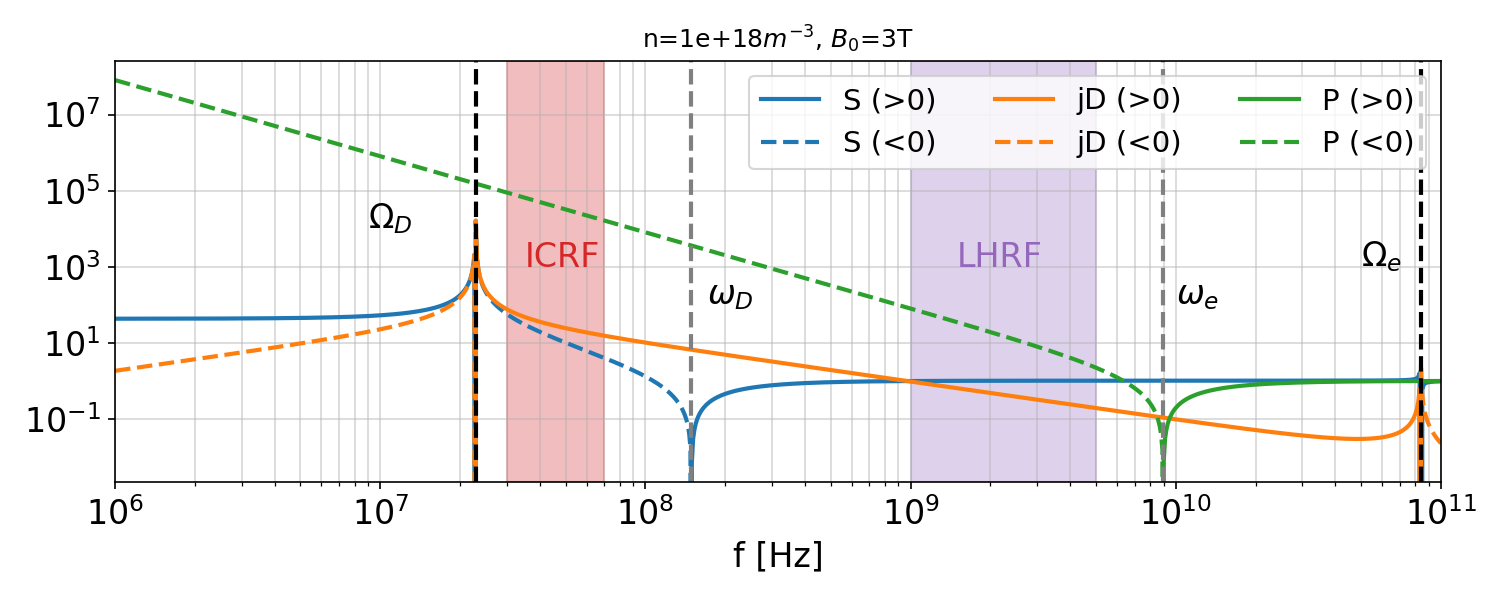
\includegraphics[width=1.0\linewidth]{figures/chap2/SDP_vs_f_nfixed_Bfixed}
	\caption{Values of the $S$, $D$, $P$ for a Deuterium plasma for density and magnetic field representative of the one we could find in front of a Tore Supra/WEST antenna. The typical Ion Cyclotron and Lower Hybrid range  of frequencies are indicated for convenience.}
	\label{fig:sdpvsfnfixedbfixed}
\end{figure*}

The form of Eq.(\ref{eq:stix_K}) is a consequence of the fact that the cold plasma is a gyrotropic media. Gyrotropic media are characterized by their invariance under any rotation about the direction of anisotropy~\sidecite{Mackay2010}, in our case the direction of the magnetic field $\Bbf_0/B_0=\mathbf{z}$. Hence, this tensor can be equivalently re-expressed into a rotation frame $(\mathbf{u}_{+}, \mathbf{u}_{-},  \mathbf{z})$, with $\mathbf{u}_{\pm}=(\mathbf{x}\pm \mathbf{y})/\sqrt{2}$:  
\begin{equation}
\Kbf(\omega)
=
\left(\begin{array}{ccc}
R & 0 & 0\\
0 & L & 0\\
0 & 0 & P
\end{array}\right)
\label{eq:stix_K_RLP}
\end{equation}
where $R$ is the \textit{right-hand} polarized component and $L$ is the \textit{left-hand} polarized component, defined as:
\marginnote{And inversely:, 
	$$
	S =  \frac{1}{2}\left(R+L\right)
	$$ 
	$$ 
	D = \frac{1}{2}\left(R-L\right)
	$$
Letters $S$, $D$, and $P$ originally come from \textit{sum}, \textit{difference} and \textit{plasma} terms \cite{stix1992}.}
\begin{subequations}
	\begin{eqnarray}
	R(\omega) 
	& = S + D = & 
	1-\sum_{s}\frac{\omega_{s}^{2}}{\omega(\omega+\Omega_{s})}
	\label{eq:stix_R}
	\\
	L(\omega)
	& = S - D = & 
	1-\sum_{s}\frac{\omega_{s}^{2}}{\omega(\omega-\Omega_{s})}
	\label{eq:stix_L}
	\end{eqnarray}
	\label{eq:stix_RL}
\end{subequations}


% ##########################################################
% ##########################################################
\subsection{Cold Plasma Dispersion Relation}
Starting from wave equation Eq.(\ref{eq:wave_equation_nxnxE}) and using that the equivalent cold plasma dielectric tensor Eq.(\ref{eq:stix_K}), one obtain:\marginnote{It is supposed that the plasma is invariant along the $\mathrm{y}$ direction, which is equivalent to say that $n_y=0$.}
\begin{equation}
\left(\begin{array}{ccc}
S - n_{z}^{2} & jD & n_{x}n_{z}\\
-jD & S - n_{x}^{2} - n_{z}^{2} & 0\\
n_{x}n_{z} & 0 & P - n_{x}^{2}
\end{array}\right)\left(\begin{array}{c}
E_{x}\\
E_{y}\\
E_{z}
\end{array}\right)=\mathbf{0}
\label{eq:relation_disp_matr_froid}
\end{equation}

The parallel direction is defined as the direction of the total confining magnetic field $\Bbf_0$. We define the \textit{parallel index} $n_\parallel$ as $n_\parallel = \mathbf{n}\cdot\Bbf_0/B_0$. We have in addition $n_{\parallel}=n_{z}$ from the frame we have defined above. The perpendicular direction is thus $n_{\perp}^{2}=n_{x}^{2}=n^{2}-n_{\parallel}^{2}$ and oriented along $\mathbf{x}$. The wavenumber spectrum in the toroidal and poloidal direction is imposed by the geometry and the RF amplitude and phase excitation of the antenna. The perpendicular index in the radial direction is then deduced from the dispersion relation, which with these notations reads to:
%\begin{marginlisting}
%Convenient \texttt{SymPy} script to obtain this result:
%\begin{lstlisting}[language=Python, basicstyle=\tiny]
%from sympy import *
%nx, ny, nz = symbols('n_x n_y n_z')
%S, D, P = symbols('S D P')
%M = Matrix([[S-nz**2, I*D, nx*nz], 
%			[-I*D, S-nx**2-nz**2, 0], 
%			[nx*nz, 0, P-nx**2]])
%M.det().factor(nx)
%\end{lstlisting}
%\end{marginlisting}

\begin{equation}
A n_{\perp}^{4} + B n_{\perp}^{2} + C = 0
\label{eq:cold_plasma_dispersion_relation_n_perp}
\end{equation}
with\marginnote[+3cm]{Where we have used $S^{2}-D^{2}=RL$.}\sidenote{NB: some signs are reversed from the solutions usually found in the literature, due to the choice of the harmonic sign $e^{j\omega t}$}:
\begin{subequations}
	\begin{eqnarray}
		A & = & S\\
		B & = & D^2 - (S - n_\parallel^2)(S + P)\\
		  & = & -RL - PS + n_{\parallel}^{2}(S+P) \nonumber \\
		C & = & P[(S - n_{\parallel}^{2})^{2} - D^2] \\
		  & = & P(n_\parallel^2 - R)(n_\parallel^2 - L) \nonumber
		\end{eqnarray}
		\label{eq:cold_plasma_dispersion_relation_n_perp_ABC}
\end{subequations}

As $S$, $D$ and $P$ do not depend on $\mathbf{n}$, Eq.(\ref{eq:cold_plasma_dispersion_relation_n_perp}) is a simple quadratic equation for $n_\perp^2$, which gives two solutions:
\begin{equation}
	n_\perp^2 
	=
	\frac{-B \pm  \sqrt{B^2 - 4AC}}{2A}
	\label{eq:nperp_solution_general}
\end{equation}
Except for some particular cases not discussed here, the discriminant $B^2 - 4AC$ is most of the time positive. This leads to two possible modes of plasma waves, called \textit{Fast} and \textit{Slow} wave modes. These names come from that the fast wave has a higher phase velocity than the slow wave. Depending on the sign of the $n_\perp^2$ solution, these waves will be either propagating ($n_\perp^2>0$) or evanescent ($n_\perp^2<0$). As seen in next sections, evanescent modes play an important role in the antenna region, in particular for coupling calculations. The antenna region is outside of the confined plasma, where the magnetic field line are open, which is called the \textit{scrape-off layer} (SOL). 


For certain values of the parameters, $n_\perp^2$ goes to zero or infinity, called \textit{cut-off} ($n_\perp^2 = 0$) or \textit{resonances} ($n_\perp^2\to\infty$) respectively \sidecite{Allis2003}. It is also possible that the two waves coalesce in a single mode, when the discriminant is zero. 
%From Eqs.(\ref{eq:nperp_solution_general}-\ref{eq:cold_plasma_dispersion_relation_n_perp_ABC}) cut-off will occur when:
%\begin{equation}
%	P = 0 \mbox{ or } R = 0 \mbox{ or } L= 0
%\end{equation}

Much of the essential physics of the wave propagation in tokamak magnetized plasma can be understood using this simplified (slab) geometry. However, so far, we have assumed that the plasma was homogenous in order to use a plane wave expansion of the electromagnetic quantities in the $(\kbf,\omega)$ domain. However, it is not the case in reality as the density and magnetic field increase as we move away from the antenna. The hypothesis that the plasma is homogeneous is similar to assuming that phenomena take place on space scale $\Delta r$ much larger than the RF wavelength. This criteria would be fulfilled if:
\begin{equation}
	\Delta r \gg \max\lambda 
	= 
	\max \frac{\lambda_0}{\sqrt{\min \varepsilon_{r}}}
	=
	\frac{\lambda_0}{\sqrt{\min\left(|S|,|D|,|P|\right)}}
\end{equation}




%which assumes that the inhomogeneity is in the $x$-direction which is also the direction of $k_\perp$. Modelling the wave in the equatorial plane of the tokamak. $k_y$ set to zero without adding anything essential to the conclusions


% ###################################################
% ###################################################
% ###################################################
\subsection{Ion Cyclotron Range of Frequencies}\label{sec:icrh}
Plasma heating of a tokamak plasma by wave coupling in the Ion Cyclotron Range of Frequencies (ICRF) requires injecting waves at a frequency $\omega$ in order to satisfy somewhere in the plasma the resonance condition\sidecite{adam1987}:
\begin{equation}
	\omega - p \Omega_i - k_\parallel v_{\parallel,i} = 0
\end{equation}
where $p$ is the cyclotron harmonic number, $\Omega_i$ the ion cyclotron angular frequency and $v_{\parallel,i}$ the parallel component of the velocity of a given species. In present tokamaks, the desired RF frequency band is around 30-70~\si{MHz}. Typical values of parameters $S$, $D$ and $P$ are illustrated in Figure~\ref{fig:icsdp}. In this range of frequency we have the ordering $\omega \ll \omega_{pe},\Omega_{ce}$ which allows to simplify a bit the previous equation. In such case, Eqs.(\ref{eq:stix_SDP}) can be further simplified for the case of a single ion species plasma to:
\marginnote{Typically, $S \ll -1$ in the plasma and change sign when crossing the so-called \textit{hybrid} resonance (where $S=0$). $D$ is mostly $\gg 1$ while $P\ll -1$. }
\begin{subequations}
	\begin{eqnarray}
		S &\approx& \frac{\omega_{i}^2}{\Omega_{i}^2 \left(1 - \omega^2/\Omega_{i}^2 \right)} \\
		D &\approx& - S \frac{\omega}{\Omega_i} \\
		P &\approx& - \frac{\omega_{e}^2}{\omega^2}  \\
		R &\approx& \frac{\omega_i^2}{\Omega_i^2 \left(1+\omega/\Omega_i\right) } \\
		L &\approx& \frac{\omega_i^2}{\Omega_i^2 \left(1-\omega/\Omega_i\right) } 
	\end{eqnarray}
\end{subequations}

\begin{figure*}[h]
	\centering
	\includegraphics[width=1.0\linewidth]{figures/chap2/IC_SDP}
	\caption{Typical values of $S$, $D$ and $P$ terms in the Ion Cyclotron Range of Frequency for the Tore Supra/WEST tokamak as a function of the electron density $n_e$ ($B_0=3\si{T}$, $f=55\si{MHz}$, $k_\parallel=9 k_0$).}
	\label{fig:icsdp}
\end{figure*}



% ###################################################
% ###################################################
\subsubsection{ICRF Dispersion Relation}
The roots of the dispersion equation Eqs.(\ref{eq:nperp_solution_general}) are approximatively\sidenote{Except close to the LH resonance} in the ICRF \sidecite{Brambilla1998, usoltceva2019}: 
\begin{subequations}
\begin{eqnarray}
n_{\perp, F}^2 &\approx& \frac{\left(R - n_\parallel^2 \right)\left(L - n_\parallel^2\right)}{S-n_\parallel^2} \\
			   &\approx& \left(S-n_\parallel^2 \right) - \frac{D^2}{S-n_\parallel^2} \nonumber \\
n_{\perp, S}^2 &\approx& \frac{P}{S}\left(S - n_\parallel^2 \right)
\label{eq:n_perp_square_approx_ICRF}		  
\end{eqnarray}
\end{subequations}
where the subscript $_F$ and $_S$ stands for \textit{Fast} and \textit{Slow} wave modes. The Figure~\ref{fig:nperpsquarevsne_ICRF} illustrates the typical range of $n_\perp^2$ values in tokamak plasma in the Ion Cyclotron Range of Frequency. 

\begin{figure*}
	\centering
	\includegraphics[width=1.0\linewidth]{figures/chap2/n_perp_square_vs_ne_ICRF}
	\caption{Perpendicular index $n_\perp^2$ from Eqs.(\ref{eq:nperp_solution_general}) (or Eqs.(\ref{eq:n_perp_square_approx_ICRF})) for Slow and Fast waves for the typical range of electron density $n_e$ found in front of tokamak ICRF antenna ($f=50\,\si{MHz}$, $B_0=3\,\si{T}$). As antennas radiate a continuous spectrum of parallel indexes $n_\parallel$, low and high values are indicated.}
	\label{fig:nperpsquarevsne_ICRF}
\end{figure*}

The Figure~\ref{fig:nperpsquarevsne_ICRF} shows that the Fast Wave mode, the one which is desired for heating the ions of the core plasma, becomes propagative for electron density beyond a \textit{cut-off} density $n_{c}$. In the ICRF, the Fast wave is evanescent up to the R-cut-off defined as: 
\begin{equation}
n_\parallel^2 = R
\end{equation}
which leads for a single ion plasma to a cut-off density $n_c$: 
\begin{equation}
	n_{e,c}
	\approx
	\frac{c^2 \varepsilon_{0} m_p}{e^2}
	\left(k_\parallel^2 - k_0^2 \right)
	\frac{\Omega_{cH}}{\omega_0}
	\left[1 + \frac{Z}{1-Z+A\omega_0/\Omega_{cH}}\right]
\end{equation}
%\begin{equation}
%n_c \approx \Omega_i^2 \frac{\left(1 + \frac{\omega}{\Omega_i}\right)}{\frac{Z^2 e^2}{\varepsilon_{0} m_i}}n_\parallel^2 
%\end{equation}
\begin{marginfigure}
	\centering
	\includegraphics[width=1.0\linewidth]{figures/chap2/core_edge_antenna}
	\caption{Illustration of the different regions in a tokamak. The core plasma is confined by following closed magnetic lines. The region defined by open field lines is the region where lie the antennas. The fast waves generated by the IC antennas are propagative only if the density is higher than a threshold, a cut-off density.}
	\label{fig:coreedgeantenna}
\end{marginfigure}
where $\Omega_{cH} = eB/m_p$, $A$ being the mass number and $Z$ the atomic number. This density depends on the RF frequency, the magnetic field and the parallel index excited by the antenna. It increases with the parallel wavenumber ($\propto k_\parallel^2$), which itself depends on the antenna phase excitation. For effective tunnelling of the Fast wave launched by the antenna, located outside the unconfined region, the plasma density in front of the antenna should be as high as possible, which highly depends on the distance between antennas and plasma. Hence, this often requires the antenna to be close as possible to the confined plasma, as illustrated in Figure~\ref{fig:coreedgeantenna}. However, this proximity has drawbacks: the heat fluxes from the plasma are impacting the antenna are higher and must be evacuated efficiently, leading to engineering issues.


% ###################################################
% ###################################################
\subsubsection{ICRF Wave Polarization}
Injecting the previous solutions into Eq.(\ref{eq:relation_disp_matr_froid}) leads to the polarization of these modes ($n_y=0$):
\begin{subequations}
	\begin{eqnarray}
		\mbox{Fast wave: } & E_z = 0 & \frac{E_x}{E_y}=\frac{j D}{S - n_\parallel^2} \\
		\mbox{Slow wave: } & E_y = 0 & \frac{E_x}{E_z}=- \frac{n_\parallel n_{\perp,S} }{S - n_\parallel^2}
	\end{eqnarray}
\end{subequations}

The key engineering issue in designing a ICRH antenna is to effectively radiate fast waves and not slow waves, as slow waves may create undesirable effects on the plasma known as \textit{RF sheaths}\sidenote{RF sheaths are briefly discussed in Section~\ref{sec:RF_sheaths}).}.

% ###################################################
% ###################################################
\subsubsection{ICRF Antennas Main Figures of Merit}
The effectiveness of Fast wave coupling is in practice measured by the maximum radiated power $P_{\mathrm{rad,max}}$ by an antenna to a given plasma and can be defined in various ways. Assuming the antenna is modelled by a lossless transmission line of characteristic impedance $Z_0$ loaded with a  resistance $R_c$, the maximum power delivered to the load would be:
\begin{equation}
P_\mathrm{rad,max} = \frac{1}{2} R_c I^2_{\mathrm{max}} = \frac{R_c}{2 Z_0^2} V_\mathrm{max}^2
\end{equation}
where $I_\mathrm{max}$ and $V_\mathrm{max}$ are the maximum peak RF current and voltage at the load. The amplitude of the maximum current on the transmission line $I_\mathrm{max}$ depends on the geometry of antenna system and of the plasma parameters. Hence, $R_c$ can be seen as a measure of the system coupling efficiency and is called the \textit{coupling} or \textit{loading} resistance. In reality however, the RF current or voltage along the strap are not constant, hence the coupling resistance can be defined using the integral over the arc length $s$ along the strap:
\begin{equation}
	R_c = \frac{2 P_{\mathrm{rad}}}{\int_s |I(s)|^2 \diff s}
\end{equation}
where $P_\mathrm{rad}$ is the time-averaged radiated power. In numerical simulation, this power can be obtained from the Poynting theorem in the $\kbf$-space as:
\begin{equation}
	P_\mathrm{rad}
	=
	\Re
	\left\{ 
	\frac{k_{0}^{2}}{4\pi^{2}}
	\iint
	\left[
	\Ebf \left(n_{y},n_{\parallel}\right)
	\times
	\Hbf^{*} \left(n_{y},n_{\parallel}\right)
	\cdot\hat{\xbf}
	\right]
	\right\} 
	\diff n_y 
	\diff n_\parallel
\end{equation}
During experiment, it can be obtained from power, voltage or current measurements, and its definition also vary from machine to machine. ICRF coupling theory is discussed in details \sidecite{messiaen1982} and compared with experiments in \sidecite{koch1988}.


The scaling of $R_c$ for an increasing electron density with a gradient length $d_c$ from the antenna to the cut-off density $n_c$,  is given by:
\begin{equation}
	R_c \propto \exp\left(- \nu \left< k_\parallel \right> d_c \right)
\end{equation}
where $\nu$ is a constant constant representing the plasma density and its gradient and $\left< k_\parallel \right>$ a characteristic factor depending on an integration over the radiated spectrum by the antenna.  On Tore Supra, this scaling has been shown to be\sidecite{clairet2004}:
\begin{equation}
R_c \propto \exp\left(- 2 \left< k_\parallel \right> d_{\mathrm{sco}} \right)
\end{equation}
where $d_{\mathrm{sco}}$ is the distance from the antenna straps to the density cut-off location. 
%KSTAR \sidecite{bae2003-1, wang2010}







% ###################################################
% ###################################################
% ###################################################
\subsection{Lower Hybrid Range of Frequencies}\label{sec:lhcd}
In the Lower Hybrid Range of Frequencies, i.e. for $\Omega_i \ll \omega \ll \Omega_e$, the $S$, $D$ and $P$ parameters can be simplified at the lead order \cite[p.222]{Brambilla1998} to (Figure~\ref{fig:lhsdp})):
\begin{subequations}
	\begin{eqnarray}
		S &\approx& 1 - \frac{\omega_i^2}{\omega^2} + \frac{\omega_e^2}{\Omega_e^2} \approx 1 \\
		D &\approx& - \frac{\omega_e^2}{\omega \Omega_e} \approx 0 \\
		P &\approx& 1 - \frac{\omega_e^2}{\omega^2} = 1 - \frac{n_e}{n_c}
	\end{eqnarray}
\end{subequations}
where $n_c$ is the cut-off density for the Slow-wave defined for $P=0$ or, more conveniently:
\begin{equation}
	n_c = \frac{m_e \varepsilon_{0}}{e^2} \omega^2 \approx  0.0124 f^2
	\label{eq:lh_cutoff_density}
\end{equation}
with $f$ specified in $\si{GHz}$ and $n_c$ given in $10^{18}\si{m^{-3}}$ 
\begin{figure*}[h]
	\centering
	\includegraphics[width=1.0\linewidth]{figures/chap2/LH_SDP}
	\caption{Values of $S$, $D$ and $P$ terms in the Lower Hybrid Range of Frequency. ($f=3.7\,\si{GHz}$,$B_0=3\,\si{T}$).}
	\label{fig:lhsdp}
\end{figure*}


% ###################################################
% ###################################################
\subsubsection{LHRF Dispersion Relation}
In the LHRF, the solution of the dispersion relation reads:
\begin{subequations}
	\begin{eqnarray}
		n_{\perp,F}^2 &\approx& S - n_\parallel^2  \approx 1 - n_\parallel^2 \\
		\label{eq:n_perp_square_FW_LHRF}
		n_{\perp,S}^2 &\approx& \frac{P}{S} \left(S - n_\parallel^2\right) \approx P(1- n_\parallel^2)
		\label{eq:n_perp_square_SW_LHRF}
	\end{eqnarray}
	\label{eq:n_perp_square_LHRF}
\end{subequations}

\begin{figure*}[h]
	\centering
	\includegraphics[width=1.0\linewidth]{figures/chap2/n_perp_square_vs_ne_LHRF}
	\caption{Perpendicular index $n_\perp^2$ from Eqs.(\ref{eq:nperp_solution_general})   for the typical range of electron density $n_e$ found in front of tokamak LHRF antenna ($f=3.7\,\si{GHz}$, $B_0=3\,\si{T}$).}
	\label{fig:nperpsquarevsne_LHRF}
\end{figure*}

% ###################################################
% ###################################################
%\subsubsection{Resonance Cone}
%Bellan and Porkolab PRL 34, 124, 1975.

% ###################################################
% ###################################################
\subsubsection{LHRF Wave Polarization}
Similarly, the electric field polarisation in the LHRF gets ($n_y=0$):
\begin{subequations}
	\begin{eqnarray}
	\mbox{Fast wave: } & E_z = 0 & \frac{E_x}{E_y}= \frac{j D}{S - n_\parallel^2} \\
	\mbox{Slow wave: } & E_y = 0 & \frac{E_x}{E_z}=- \frac{n_\parallel n_{\perp,S} }{S - n_\parallel^2}
	\end{eqnarray}
\end{subequations}

% ###################################################
% ###################################################
\subsubsection{Wave propagation conditions}
In order for the RF power to reach the plasma core, the excited waves by a LHCD launcher must satisfy different criteria: 

\begin{itemize}
	\item  A \emph{cut-off condition}: the electron density in front of the launcher must be close or higher than the slow-wave electron \emph{cut-off density}, given by Eq.(\ref{eq:lh_cutoff_density}), that increases as the square of the source frequency. 
	\item A propagation condition: in order for the Slow and Fast waves in the LHRF to propagate into the magnetized plasma, from Eqs.(\ref{eq:n_perp_square_LHRF}) excited waves must have an absolute value of the parallel index greater than one, i.e. $|n_{\parallel}|>1$ 
	\item An accessibility condition: in order for the Slow waves accessing the plasma core to not be mode-converted into Fast waves, a minimum value of $n_{\parallel}$ for a given plasma density and magnetic field is requested\sidecite{golant1972}:
	\begin{equation}
	|n_{\parallel} |>| n_{\parallel \mathrm{access}} | 
	\approx 
	\sqrt{1 
		- \frac{\omega_{pi}^2}{\omega^2} 
		+ \frac{\omega_{pe}^2}{\omega_{ce}^2}}
	+ \frac{\omega_{pe} }{| \omega_{ce} |}
	\label{eq:accessibilit_condition_LH}
	\end{equation}
\end{itemize}

When the accessibility condition is satisfied, the Slow and Fast branches of the dispersion relation are separated and the LH waves can reach the core plasma. Inversely, for a given $n_{\parallel}$, the previous condition leads to an upper limit for the density (inside the plasma), above which the wave can’t propagate.

% ###################################################
% ###################################################
\subsubsection{LHRF Antennas Main Figures of Merit}
There are three important figures of merit to measure the efficiency and
performance of a LH launcher. The first one is the $\mathbf{k}$-space radiated power spectrum density $ p(n_y, n_\parallel)$, defined as the $k$-space Poynting vector\marginnote{Integrating the power spectrum density over the entire $n$-space gives the transmitted power to the plasma.}:
\begin{equation} 
 p
\left(n_{y},n_{\parallel}\right)
=\Re\left\{ \frac{k_{0}^{2}}{4\pi^{2}}
\left[\tilde{\mathbf{E}}
\left(n_{y},n_{\parallel}\right)
\times
\tilde{\mathbf{H}}^{*}\left(n_{y},n_{\parallel}\right)
\cdot\hat{\xbf}
\right]
\right\} 
\end{equation}
Since it is often assumed that the plasma is infinite in the $y$ direction (slab model), the main acceptation of the power spectrum density is $ p(n_\parallel)$, which corresponds to integrate the contribution of all the $n_{y}$ for a given $n_{\parallel}$:
\begin{equation}
 p\left(n_{\parallel}\right)=\int_{-\infty}^{+\infty}\!  p\left(n_{y},n_{\parallel}\right)\, \diff n_y
\end{equation}
This quantity represents the amount of power excited by the launcher for each parallel index $n_\parallel$. % The relation between this power spectrum and the array excitation is related to the Fourier transform of the electromagnetic field at the plasma-antenna interface.

The second one is the ratio of the reflected power (at the mouth or at the end of the launcher) to the input power, named the reflection coefficient $|\Gamma|^2 $ and often expressed in percent:
\begin{equation}
	|\Gamma|^2 = P_r/P_i
\end{equation} 

The third one is the directivity of the launcher, which is the fraction of the power spectrum over its total power content. It can be viewed as the fraction of the power that goes toward one toroidal direction over the total coupled power. One can define the directivity as:
\begin{equation}
\mathrm{Dir} = \frac{\int_{n_\parallel > 0}   p(n_\parallel) \diff n_\parallel}{\int  p(n_\parallel) \diff n_\parallel} 
\end{equation}

Since the wave field at the launcher aperture (and thus the launcher spectrum) depends on both the antenna and the plasma, numerical coupling codes are required to make a self-consistent numerical evaluation of the coupling. Different types of launchers have been developped to balance the sometimes conflicting requirements of experimental flexibility, reduced complexity and thermal constraints. These antennas are discussed in Section~\ref{sec:LHCD_antennas_general}.


%The RF power is coupled by the launcher to the plasma, which means that the electromagnetic waves in the launcher’s waveguides are converted to (mainly) slow waves in the plasma. In the LH range of frequencies (~2 to 8 GHz), the wavelength of the RF waves in the plasma is well below the typical beam size, which itself is smaller than the equilibrium non-uniformity scale. It this situation, the evolution of the waves in the plasma can be described by the \emph{ray-tracing} formalism. Since the evolution of the electron population can be described with Fokker-Planck calculation, the combination of the both tools is standard for modelling LHCD experiments\sidecite{bonoli1982, peysson2012}.
%
%As said before, the LHCD launcher is a phased array of waveguide which excites a slow plasma wave. The following calculations taken from current drive theory illustrate the basic requirements of the LHCD launcher in order to optimize the current drive efficiency. 
%
%In the plasma, the incremental current $\Delta j$ carried by an electron of electrical charge $q=-e$ and accelerated from a parallel velocity $v_\parallel$ to $v_\parallel + \Delta v_\parallel$ is:
%$$\Delta j = q \Delta v_{\parallel}$$
%
%The incremental increase of kinetic energy is:
%$$\Delta E = m v_{\parallel} \Delta v_{\parallel}$$
%
%Eliminating $\Delta v_{\parallel}$ leads to an incremental current: 
%$$\Delta j = \Delta E \; q/(m v_{\parallel})$$ 
%
%Let $\nu_\mathrm{coll}$ be the Coulomb collisional frequency. At first order \footnote{Rigourously, the mathematical tool for a complete description of multiple scattering processes in the velocity-space is the Boltzman equation. The collision term modelling the multiple particles Coulomb collisions in this equation can be modelled by a collision term of the Fokker-Planck type.} the incremental energy input $\Delta E$ persists for a time $1/\nu_\mathrm{coll}$. The associated (steady-state) RF input power $\Delta P$ required is thus: 
%$$\Delta P = \nu_\mathrm{coll} \Delta E$$ 
%
%From the two previous equations, the ratio of the incremental current to the RF input power is:
%$$\Delta j/ \Delta P = q / (m \nu_\mathrm{coll} v_{\parallel})$$
%
%This suggests that more current can be driven with low parallel velocity electrons. However, fast electrons collide less often than slower, as the Coulomb collision cross section falls off with increasing relative velocity as $\nu_\mathrm{coll} \propto n_e/v_{\parallel}^3$ (for parallel velocity larger than the thermal velocity). It follows that the previous ratio is proportional to: 
%
%$$\Delta j/ \Delta P \propto (v_{\parallel}^2 q) / (m n_e)$$
%
%this means that high current drive efficiency can be reached from fast electrons. Thus, it is actually more effective to push fast electrons than slower. Even if it may be energetically more expensive to accelerate fast electrons, this energy deposition need occurs less often because current last longer when carried by relatively less collisional electrons \sidecite{fisch1987}. 
%
%For the purpose of current drive with LH waves, the Landau damping is the dominant absorption mechanism. Landau damping is a collision-less damping process in which particles exchange energy with waves travelling with the nearly same phase velocity parallel to the magnetic field, that is, for particle parallel velocity $v_{\parallel}$ satisfying resonant condition:
%
%$$\omega – k_{\parallel} v_{\parallel} = 0 $$ 
%
%where $k_{\parallel}=k_0 n_{\parallel}$ is the parallel wavenumber of the wave, $n_{\parallel}$ the parallel index of refraction and $k_0= \omega/c$ the wavenumber in vacuum. From the previous relation one deduces that the LHCD launcher must excite waves satisfying the resonant condition $v_{\parallel}=c/n_{\parallel}$. As for the slow wave to be able to penetrate into the plasma the parallel index must be greater than one and also greater to $|n_{\parallel \mathrm{access}}|$, typical LHCD launchers in current tokamaks excite a main parallel index between $n_{\parallel 0}$=1.5 to 3.0. 
%
%However, in many past and present LHCD experiments, the resonant velocity $v_{\parallel 0}=c/n_{\parallel 0}$ corresponds to supra thermal region where the number of electrons should be in principle too small for any significant wave damping to take place and to account for the observed current drive. Indeed, strong wave damping on a Maxwellian distribution with temperature $T$ requires the wave damping to be no larger than four times the thermal velocity $v_T=\sqrt{k T/m}$. This paradox is commonly referred to as the \emph{spectral gap} problem and is an active area of research. Various explanations are proposed to explain this spectral gap, among these the toroidal effects on the wave propagation that can cause sufficient up-shift (increase of the parallel wavenumber) in the parallel refraction index $n_{\parallel}$ to “fill” the spectral gap, non-linear interactions such as \textit{parametric decay instabilities} (PDI), diffraction effects or power density spectrum fluctuations. 



\clearpage
% ###################################################
% ###################################################
\section{The ALOHA code}\label{sec:ALOHA}
\marginnote{Parts of this section are taken from paper \citeauthyear{hillairet2010}.}
% ###################################################
\subsection{Context of this work}
The theory of the coupling between LHRF antennas and the plasma has been developed in \sidecite[-0.5cm]{brambilla1976-1,brambilla1979} for 2D waveguides (parallel plates infinite the poloidal direction) and refined after for rectangular waveguides in \sidecite{bers1983}. In 2007, best known linear coupling codes used to design present operating antennas are Slow Wave ANtenna (SWAN) \sidecite{litaudon1990, moreau1984} or GRILL3D \sidecite[+1cm]{irzak1995}. In these codes, the toroidal lines of waveguides are assumed to be infinite in the poloidal direction and are described using a modal expansion. The modal description of the field makes possible to simulate large antennas with a moderate computing cost but the code cannot handle realistic geometry.

In order to improve the antenna-plasma coupling description of SWAN code while keeping its low computational cost, a code named Advanced LOwer Hybrid Antenna (ALOHA) has been developed\sidenote{The code has been initially written by S.Berio and Ph.Bibet in 1994 \cite{berio1996}, then improved later by Damien Voyer in 2006. Since 2008, I continued to develop the code, completely rewritten since in modern Fortran with a Matlab front-end. The code development was first versioned on CEA internal servers since Nov.2009 before being \href{https://github.com/jhillairet/ALOHA}{open-sourced in on github} since Sept.2015. ALOHA has been used by different user in fusion laboratory worldwide: MIT/PSFC, ASIPP, NFRI, IPR, IPP/Prague, etc. Since 2008, ALOHA has been cited in more than 130 references.}. In ALOHA, LH antennas may be modelled by any RF full-wave commercial software or home-made code\footnote{For optimization process, a plug-in named HAMAC (Hybrid Antenna Modelling for the ALOHA Code) has been developed in the frame of the master training of Melanie Preynas in 2009 and Michal Kazda in 2010.}. The plasma coupling is calculated from a fast classical 1D modelling that describes the effect of the slow wave only\cite{brambilla1976-1} or from a more advanced 2D modelling that implies the contribution of both fast and slow waves\cite{brambilla1979, bers1983, irzak1995}.
These calculations are based on the linear cold plasma theory and non-linear effects, such as thermal effects ("warm" dielectric tensor) and ponderomotive force have not been taken into account in the present analysis. However, some specific developments have been brought in one hand, to describe a more realistic electron density profiles taking into account the close environment of LH antennas and in the other hand, to avoid computational difficulties when the antenna is large. These assumptions let ALOHA to solve a case in a couple of seconds up to 2 hours on a 2008 desktop computer, depending on the number of waveguides of the antenna and the plasma model chosen. By comparison, a boundary element code such as the Torino Politecnico Lower Hybrid Antenna (TOPLHA) code\sidecite{milanesio2011}, required at that time high-end or super-computers to be solved. At the same time, finite element software such as COMSOL just began to be able to treat materials with generic temporally-dispersive dielectric tensors. Such approach leaves absolute freedom in the description of the antenna geometry and of the plasma within the collisional cold plasma approximation but required high computation time or resources \sidecite{meneghini2009-1, shiraiwa2011-1}. Nowadays, the Finite-Element Method can be used in more daily basis for LHCD coupling as discussed in Section~\ref{sec:LHCD_FW_antena_coupling}. However, it is still incompatible with intensive use, for example in daily experiments when one has to evaluate the effect of modules tripping on the radiated spectrum or during antenna design stage, where many calculations may be expected. In order to interpret and improve present day experiments and to design future antennas, an advanced but fast and convenient modelling tools is still convenient.

The next section recalls the key elements of the linear coupling theory. ALOHA specificities are detailed, such as the use of generalized scattering matrix, the 2D grill modelling and the two electron density gradients profile. Section~\ref{sec:ALOHA_TS} is devoted to experimental comparisons and simulation benchmarks on Tore Supra antennas. 


\subsection{Main assumptions}\label{sec:Theory}

\subsubsection{Network description}\label{sec:network_description}

The LHCD antennas of past or present experiments (JET, Alcator C-Mod, FTU, EAST, KSTAR, Tore Supra/WEST, etc.) are designed to launch an asymmetric parallel wavenumber spectrum where most of the power is generated at a low parallel refractive index $\left|n_{\parallel}\right|\approx2$. This is usually achieved by phasing the forward waves in waveguides that are stacked along the static magnetic field. This phasing can be obtained externally in the transmission line feeding of the antenna \sidecite[-2cm]{bernabei2003, bae2003, park2010} or directly inside the antenna when E-plane power dividers -- usually called "multijunction" \sidecite{moreau1984} -- are associated with built-in phase shifters \sidecite[+0.5cm]{ekedahl2009-1, bo-jiang2006, zhao2010}.

Here, the term "module" refers to the unit of the antenna composed of one "input" waveguide fed by the power source and one or several "output" waveguides facing the plasma, and the "grill" refers to the plane containing all the open ended waveguides of the antenna. A complete LH antenna can be made of many different modules, stacked in the toroidal or poloidal directions. A simple example is depicted in Figure~\ref{fig:geometry_antenna}.

In the ALOHA code, the plasma coupling of a LH grill antenna is split into two parts: the modeling of the modules and the modeling of the grill in front of the plasma. 

Firstly, the electromagnetic characterization of a module is obtained using some RF software or code, which results in the calculation of the scattering matrix of a module $\mathbb{S}_{\mbox{module}}$ in which only the propagating modes are taken into account. This matrix quantifies the coupling between all inputs and outputs of the RF structure \cite{kurokawa1965}. 

Secondly, the coupling to the plasma of all the output waveguides that compose the grill is considered. At this stage, evanescent modes excited at the end of the waveguides are also taken in account. Thus, the grill is characterized by a $N$-port network where $N=N_{\mbox{wg}}\times N_{\mbox{modes}}$ is the number of ports, $N_{\mbox{wg}}$ the total number of output waveguides and $N_{\mbox{modes}}$ the number of electromagnetic modes in each waveguide. A scattering matrix $\mathbb{S}_{\mbox{grill/plasma}}$ of dimensions $N\times N$ is then derived using the approach detailed in Section~\ref{sec:grill_modeling}: this matrix quantifies the coupling between the different ports. In such a modeling, each mode is associated to a port \cite{Harrington2001}; a port can coincide either with the principal mode that propagates inside an output waveguide or with a higher order mode excited at the end of an output waveguide. 

Finally, following the well known network approach, both modellings are combined: the ports in the scattering matrices $\mathbb{S}_{\mbox{module}}$ and $\mathbb{S}_{\mbox{grill/plasma}}$ that correspond to the same mode in a waveguide are identified and the global response of the antenna can then be extracted and directly compared to experimental data.

For a better understanding, let us consider the example of the antenna shown in Figure~\ref{fig:geometry_antenna}. It is composed of one toroidal line of waveguides shared into two modules. Each module is a multijunction in which a large input feeding waveguide is split into four smaller output waveguides; the output waveguides are said to be active waveguides since they are connected to the input waveguide inside the module. The modules are separated by a short circuited waveguide; this waveguide is isolated and consequently is said to be passive. Moreover, there is also one passive waveguide on each side of the antenna. Each module is characterized by a scattering matrix $\mathbb{S}_{\mbox{module1}}$ and $\mathbb{S}_{\mbox{module2}}$.

%
\begin{figure}[h]
	\centering{}\includegraphics[width=0.9\textwidth]{figures/chap2/ALOHA/figure1} 
	\caption{A typical LH (multijunction) antenna structure. In this example, the
		antenna is made of two multijunction modules stacked in the toroidal
		($z$) direction. One passive waveguide is inserted between both modules
		and on each side of the antenna.\label{fig:geometry_antenna} }
	
\end{figure}


Suppose that, in front of the plasma, two modes are excited inside the output waveguides: the principal mode $\TE_{10}$ and the evanescent mode $\TM_{11}$. The network modeling of this problem is given in figure \ref{fig:network_representation}. In that representation, a port in a N-port network is described by a terminal. Thus, each of both modules is characterized by a 5-port network (1\,input waveguide $\times$ 1\,mode + 4\,active waveguides $\times$ 1\,mode) and the coupling of the grill with the plasma is modeled by a 22-port network (\textit{\emph{8\,active waveguides $\times$ 2\,modes + 		3\,passive waveguides $\times$ 2\,modes}}). The terminals in the 22-port network that coincide with the principal mode of the active waveguides in the modules are connected to the corresponding terminals in the 5-port network. The terminals in the 22-port network that coincide with the principal mode of the passive waveguides are shunt on a piece of transmission line ended by a short-circuit to model the reflection of the wave. The terminals in the 22-port network that coincide with the evanescent modes are shunt on the imaginary mode impedance of the output waveguide, which is equivalent to consider that those modes carry reactive energy in a waveguide of infinite length. Finally, the antenna reduces to a 2-port network in which the ports correspond to the input feeding waveguide of both modules and the global scattering matrix of the antenna is a $2\times2$ matrix $\left(\mathbb{S}_{\mbox{access}}\right)$. This formalism allows the code to fully take into account the coupling of the modes in the waveguides.

%
\begin{figure}[h]
	\centering{}\includegraphics[width=0.7\textwidth]{figures/chap2/ALOHA/figure2} \caption{Illustration of the modeling of the antenna described in figure \ref{fig:geometry_antenna}
		using the N-port concept.\label{fig:network_representation} }
	
\end{figure}



\subsubsection{Module modelling}\label{sub:module_modeling}

Lower Hybrid experiments show that the coupling efficiency not only depends on the plasma configuration but also on the antenna structure. Antennas are often designed in order to minimize the reflected power from the plasma to the RF sources, thus limiting the need of complex and expensive klystron protection systems. Multijunction concept is frequently used in tokamaks in order to create large waveguide arrays. The necessary phase shifts between adjacent waveguides used to launch non-symmetrical parallel wavenumber spectrum is usually obtained in the design by adjusting the relative guide heights \sidecite{litaudon1992}. These built-in phase shifters create multiple passages of the waves through the structure, which lead to a reduction of the reflected power to the RF sources as well as an increase of the electric field strength or an increase of secondary peaks in the radiated power spectrum. Thus, the RF design of such antennas is less straight-forward than simple open-ended waveguides and an accurate RF characterization is required to analyze the experimental data.

The coupling efficiency requires the measurement of the forward and reflected electric fields in all waveguides which in principle can be done but requires the installation under vacuum of a very large number of probes\sidecite{jacquet1997, meneghini2010}. For an easier maintenance of the RF system, the use of a single bi-directional coupler at the module input in the pressurized transmission line is usually preferred. With this scheme, the electric field map at the plasma-antenna interface, needed to compute the launched parallel index $n_{\parallel}$, is only accessible by computation. In order to directly compare theoretical coupling predictions to experimental RF measurements, the RF description of each module have to be considered incorporating all the RF components in line from the plasma up to the RF probes location. Thus, the realistic wave propagation inside each module, through multijunctions and power splitters (such as hybrid junctions, magic tees or mode converters) has to be taken into account. 

Commercial RF softwares, for example ANSYS HFSS, CST Studio or COMSOL, are convenient tools to design and optimize such components. In ALOHA, the scattering matrix calculated by these codes that describe the modules of the antenna can be directly used as input. Once the antenna's module scattering matrices calculated ($\mathbb{S}_{\mbox{module}}$), they are used as input for ALOHA to simulate the coupling between the modules and the plasma, as explained in the next sections.


\subsubsection{Grill-plasma modelling}\label{sec:grill_modeling}

\paragraph{Plasma description}\label{sec:dielectric_tensor}

Lets consider the geometry shown in Figure~\ref{fig:geometry_antenna}. The static magnetic field $\mathbf{B}_{0}$ is assumed to be in the $z$ direction and vary as well as the plasma density in $x$ direction. This hypothesis is specifically valid for large tokamak such as ITER or tokamak with large aspect ratio in which the angle between the magnetic field and the narrow waveguide is small. The interface between waveguides and plasma is set at $x=0$. The plasma is considered homogeneous
in $y$ and $z$ directions. The electromagnetic field scattered by the antenna is supposed to be dissipated far away from the coupling region so that the coupling problem is treated as a problem of radiation in a semi-infinite medium independently of the absorption in the core plasma. In such a modelling, the propagation into the plasma core is not calculated, meaning that effects such as mode conversion are not taken into account. 

From Maxwell's equations, we recall that the electromagnetic field in a cold plasma in the absence of source satisfies the vector wave equation:
\begin{equation}
\left(\nabla\times\nabla\times-k_{0}^{2}\mathbf{K}\cdot\right)\left|\begin{array}{c}
\mathbf{E}(\mathbf{r})\\
\mathbf{H}(\mathbf{r})\end{array}\right.=0
\end{equation}

where $\mathbf{E}$ and $\mathbf{H}$ are the electric and magnetic fields, $\mathbf{r}=x\mbox{\ensuremath{\hat{\mathbf{x}}}}+y\hat{\mathbf{y}}+z\hat{\mathbf{z}}$ is the space vector coordinates and $k_{0}=\frac{\omega}{c}$ the free-space wavenumber. In the vicinity of the grill, the plasma is described by its (normalized) cold dielectric tensor $\mathbb{K}$ Eq.(\ref{eq:stix_K}) which is recalled here: 
\begin{equation}
	\mathbf{K}(x,\omega)=\left[\begin{array}{ccc}
	S & jD & 0\\
	-jD & S & 0\\
	0 & 0 & P\end{array}\right]
	\label{eq:dielectric_tensor}
\end{equation}
where parameters $S$, $D$ and $P$ are defined by Eq.(\ref{eq:stix_SDP}) and depend on radial position $x$ and wave frequency.

%\begin{eqnarray}
%S(x,\omega) & = & 1-\sum_{s}\frac{\omega_{p,s}^{2}}{\omega^{2}-\Omega_{c,s}^{2}}\label{eq:stix_sum}\\
%D(x,\omega) & = & \sum_{s}\frac{\Omega_{ci}}{\omega}\frac{\omega_{p,s}^{2}}{\omega^{2}-\Omega_{c,s}^{2}}\label{eq:stix_difference}\\
%P(x,\omega) & = & 1-\sum_{s}\frac{\omega_{p,s}^{2}}{\omega^{2}}\label{eq:stix_plasma}
%\end{eqnarray}
%where $\omega$, $\Omega_{c,s}$ and $\omega_{p,s}$ are respectively the RF source, the cyclotron and the plasma angular frequencies of the species $s$.

% ####################################################################
\paragraph{Grill description}
The transverse (perpendicular to the $x$ direction) electromagnetic field $\mathbf{E}_{t,\mbox{grill}}$, $\mathbf{H}_{t,\mbox{grill}}$ at the end of the output waveguides, i.e. in the $x=0$ grill plane, can be expanded as a series of excited modes in similar way than Eq.(\ref{eq:voltage_current_lossy_line}) from Chap.\ref{chap:RF_fundamentals}:
\begin{eqnarray}
\mathbf{E}_{t,\mbox{grill}}(x=0,y,z) & = & \sum_{n=1}^{N}\sqrt{Z_{n}}\left(a_{n}+b_{n}\right)\mathbf{e}_{t,n}(y,z)\\
\mathbf{H}_{t,\mbox{grill}}(x=0,y,z) & = & \sum_{n=1}^{N}\frac{1}{\sqrt{Z_{n}}}\left(a_{n}-b_{n}\right)\mathbf{h}_{t,n}(y,z)
\end{eqnarray}
where $\mathbf{e}_{t,n},\,\mathbf{h}_{t,n}$ are the TE or TM modal functions (explicitly given in reference.\,\cite{Harrington2001}) associated to the port $n$ and $Z_{n}$ the impedance of the port $n$ for the current mode. The coefficients $a_{n}$ and $b_{n}$ are the incident and reflected power waves associated to the port $n$. We recall that $N=N_{\mbox{wg}}\times N_{\mbox{modes}}$ is the total number of ports, $N_{\mbox{wg}}$ being the total number of waveguides and $N_{\mbox{modes}}$ the number of modes in each waveguide. Since the analytical expression of the modes function $\mathbf{e}_{t,n},\,\mathbf{h}_{t,n}$ are known, the transverse fields can be analytically expressed in the spectral domain by Fourier transform:
\begin{eqnarray}
\tilde{\mathbf{E}}_{t,\mbox{grill}}\left(n_{y},n_{z}\right) & = & \sum_{n=1}^{N}\sqrt{Z_{n}}\left(a_{n}+b_{n}\right)\tilde{\mathbf{e}}_{t,n}\left(n_{y},n_{z}\right)\label{eq:E_grill_spectral}\\
\tilde{\mathbf{H}}_{t,\mbox{grill}}\left(n_{y},n_{z}\right) & = & \sum_{n=1}^{N}\frac{1}{\sqrt{Z_{n}}}\left(a_{n}-b_{n}\right)\tilde{\mathbf{h}}_{t,n}\left(n_{y},n_{z}\right)\label{eq:H_grill_spectral}\end{eqnarray}
where $\tilde{\mathbf{e}}_{t,n}$ and $\tilde{\mathbf{h}}_{t,n}$ are the Fourier transform of the modal functions $\mathbf{e}_{t,n},\,\mathbf{h}_{t,n}$ and $n_{y}=k_{y}/k_{0}$ and $n_{z}=k_{z}/k_{0}$ are the refractive indexes in $y$ and $z$ directions respectively. These latter expressions will be used for the coupling calculation in the next section.


\paragraph{Coupling from grill to plasma}

Following the classical linear-coupling regime \cite{brambilla1979,bers1983}, the characterization of the plasma medium can be reduced to a spectral surface admittance $\mathbb{Y}_{S}$ defined on the plane that separates the grill from the plasma region:
\begin{equation}
\tilde{\mathbf{H}}_{t,\mbox{plasma}}\left(n_{y},n_{z}\right)=Y_{0}\mathbb{Y}_{S}\left(n_{y},n_{z}\right)\tilde{\mathbf{E}}_{t,\mbox{plasma}}\left(n_{y},n_{z}\right)\label{eq:surface_admittance}
\end{equation}

where $\tilde{\mathbf{H}}_{t,\mbox{plasma}}\left(n_{y},n_{z}\right)$ and $\tilde{\mathbf{E}}_{t,\mbox{plasma}}\left(n_{y},n_{z}\right)$ are the Fourier transforms of the transverse magnetic $\mathbf{H}_{t,\mbox{plasma}}(x=0,y,z)$ and electric fields $\mathbf{E}_{t,\mbox{plasma}}(x=0,y,z)$. $Y_{0}$ is the vacuum admittance. The plasma surface admittance $\mathbb{Y}_{s}$, which is discussed in Sec.\ref{sec:surface_admittance}, is generally
a $2\times2$ complex matrix.

The waveguides of the grill are supposed to be opened through a perfect metallic surface of infinite extent. Due to the continuity of the transverse electric field in the waveguide openings and no tangent electric field on the perfect metallic surface, the transverse magnetic field $\tilde{\mathbf{H}}_{t,\mbox{plasma}}$ can be expressed using the surface admittance $\mathbb{Y}_{s}$ defined in (\ref{eq:surface_admittance}) and the expansion of the electric field $\tilde{\mathbf{E}}_{t,\mbox{grill}}$ given in (\ref{eq:E_grill_spectral}). Thus, 
\begin{equation}
\tilde{\mathbf{H}}_{t,\mbox{plasma}}\mbox{\ensuremath{\left(n_{y},n_{z}\right)}}=\sum_{n=1}^{N}\sqrt{Z_{n}}\left(a_{n}+b_{n}\right)Y_{0}\mathbb{Y}_{s}\left(n_{y},n_{z}\right)\tilde{\mathbf{e}}_{t,n}\left(n_{y},n_{z}\right)\label{eq:H_plasma_spectral}
\end{equation}

Let $\tilde{\mathbf{H}}_{t,\mbox{metal}}\left(n_{y},n_{z}\right)$ be the transverse magnetic field related to the current induced on the perfect metallic surface of infinite extent. Due to the continuity between transverse magnetic field in the waveguide openings, one finds from the expansion of the magnetic field in the grill (\ref{eq:H_grill_spectral}) and in the plasma (\ref{eq:H_plasma_spectral}) the following equality:
\begin{eqnarray}
\sum_{n=1}^{N}\frac{1}{\sqrt{Z_{n}}}\left(a_{n} - b_{n}\right)\tilde{\mathbf{h}}_{t,n}\left(n_{y},n_{z}\right) & + & \tilde{\mathbf{H}}_{t,\mbox{metal}}\left(n_{y},n_{z}\right)=\label{eq:H_continuity_spectral}\\
&  & \sum_{n=1}^{N}\sqrt{Z_{n}}\left(a_{n}+b_{n}\right)Y_{0}\mathbb{Y}_{s}\left(n_{y},n_{z}\right)\tilde{\mathbf{e}}_{t,n}\left(n_{y},n_{z}\right)\nonumber 
\end{eqnarray}

The mode matching method is then applied \cite{berio1996}: a linear system is obtained by dot product multiplying both sides of (\ref{eq:H_continuity_spectral}) with $\tilde{\mathbf{h}}_{t,m}^{*}\left(n_{y},n_{z}\right)$ for $m=1,\ldots,N$ and integrating over the spectral domain $\left\{ n_{y},n_{z}\right\} $ of infinite extent. Moreover, by multiplying both sides by $k_{0}^{2}/4\pi^{2}$, the left hand side of the equation can be transposed in the spatial domain $\left\{ y,z\right\} $ thanks to Parseval's theorem:
\begin{eqnarray}
\sum_{n=1}^{N}\frac{1}{\sqrt{Z_{n}}}\left(a_{n}-b_{n}\right)\left[\int\int_{-\infty}^{+\infty}\!\mathbf{h}_{t,m}^{*}\left(y,z\right)\cdot\mathbf{h}_{t,n}\left(y,z\right)\, dy\, dz\right.\\
\left.+\int\int_{-\infty}^{+\infty}\!\mathbf{h}_{t,m}^{*}\left(y,z\right)\cdot\mathbf{H}_{t,\mbox{metal}}\left(y,z\right)\, dy\, dz\right]=\nonumber \\
\sum_{n=1}^{N}\sqrt{Z_{n}}\left(a_{n}+b_{n}\right)C_{mn}\nonumber 
\end{eqnarray}
where the coupling admittance term $C_{mn}$ is given by:
\begin{equation}
C_{mn}=Y_{0}\frac{k_{0}^{2}}{4\pi^{2}}\int\int_{-\infty}^{+\infty}\tilde{\mathbf{h}}_{t,m}^{*}\left(n_{y},n_{z}\right)\mathbb{Y}_{s}\left(n_{y},n_{z}\right)\tilde{\mathbf{e}}_{t,n}\left(n_{y},n_{z}\right)\, dn_{y}\, dn_{z}\label{eq:coupling_admittance}
\end{equation}
Since the modal function $\mathbf{h}_{t,m}$ is zero on a perfect metallic plane, the term involving $\mathbf{H}_{t,\mbox{metal}}$ cancels. The orthonormal properties of the modal eigenfunctions\cite{Collin1990,Harrington2001}
leads to:
\begin{equation}
\frac{1}{\sqrt{Z_{m}}}\left(a_{m}-b_{m}\right)=\sum_{n=1}^{N}\sqrt{Z_{n}}\left(a_{n}+b_{n}\right)C_{mn}\qquad\forall\, m=1,\,\ldots,\, N\label{eq:linear_system}
\end{equation}
The linear system of equation.(\ref{eq:linear_system}) can be rewritten
using a matrix formalism:
\begin{equation}
\sqrt{\mathbb{Z}}^{-1}\left(\mathbf{a}-\mathbf{b}\right)=\mathbb{C}\sqrt{\mathbb{Z}}\left(\mathbf{a}+\mathbf{b}\right)\label{eq:linear_system_matrix}
\end{equation}
where $\sqrt{\mathbb{Z}}$ is diagonal matrix with $\left[\sqrt{\mathbb{Z}}\right]_{ii}=\sqrt{Z_{i}}$ and $\mathbb{C}$ is the coupling admittance matrix with $\left[\mathbb{C}\right]_{ij}=C_{ij}$. $\mathbf{a}$ and $\mathbf{b}$ are respectively the incident and reflected waves vectors associated to the port $i$, such as $\left[\mathbf{a}\right]_{i}=a_{i}$ and $\left[\mathbf{b}\right]_{i}=b_{i}$. The scattering matrix $\mathbb{S}_{\mbox{grill/plasma}}$ discussed in Section~\ref{sec:network_description} is defined by

\begin{equation}
\mathbf{b}=\mathbb{S}_{\mbox{grill/plasma}}\mathbf{a}\label{eq:Sgrillplasma_def}
\end{equation}
Finally, using (\ref{eq:linear_system_matrix}), one finds:
\begin{equation}
\mathbb{S}_{\mbox{grill/plasma}}=\left(\mathbb{I}+\sqrt{\mathbb{Z}}\mathbb{C}\sqrt{\mathbb{Z}}\right)^{-1}\left(\mathbb{I}-\sqrt{\mathbb{Z}}\mathbb{C}\sqrt{\mathbb{Z}}\right)
\end{equation}
where $\mathbb{I}$ is the unit matrix.

\subsection{Antenna power spectrum}
An important feature of LH antennas is the radiated power spectral density $p$ that can be computed from the Poynting vector: 
\begin{equation} 
 p
\left(n_{y},n_{z}\right)
=\Re\left\{ \frac{k_{0}^{2}}{4\pi^{2}}\left[\tilde{\mathbf{E}}\left(n_{y},n_{z}\right)\times\tilde{\mathbf{H}}^{*}\left(n_{y},n_{z}\right)\cdot\widehat{x}\right]\right\} 
\label{eq:power_spectrum_2D}
\end{equation}
According to previous equations, this power density can be evaluated once the power waves $\mathbf{a},\mathbf{b}$ for each waveguides have been calculated. In order to compare 1D and 2D modelling, it is possible to define a 1D spectrum $p_{z}$ that integrates the contribution of all the $n_{y}$ for a given $n_{z}$:
\begin{equation}
p_{z}\left(n_{z}\right)
=
\int_{-\infty}^{+\infty}\! 
p\left(n_{y},n_{z}\right)\, \diff n_{y}
\label{eq:power_spectrum_1D}
\end{equation}
Finally, the power conservation must imply that, neglecting the RF
losses in the antenna:
\begin{equation}
\int\int_{-\infty}^{+\infty}\! 
p\left(n_{y},n_{z}\right)\, dn_{y}\, \diff n_{z}
=
\sum_{n=1}^{N_{\mbox{module}}}p_{n,\mbox{in}}\left(1-RC_{n}\right)
\label{eq:spectrum_power_conservation}
\end{equation}
where $p_{n,\mbox{in}}$ and $RC_{n}$ are respectively the power incoming from an RF source and the Reflection Coefficient for the n-th module. 


\subsection{Plasma surface admittance}\label{sec:surface_admittance}

The plasma surface admittance defined in equation.(\ref{eq:surface_admittance}) can be evaluated either numerically or analytically depending on the hypothesis made on the wave propagation plasma and on the density
profile\cite{brambilla1979, bers1983}. In ALOHA, two kinds of wave propagation models have been implemented. 

In the first one, the so-called ALOHA-2D mode -- 2D because the plasma parameters depend on two coordinates, namely $n_{y}$ and $n_{z}$ -- waveguides cross-section are considered finite in both dimensions and both TE and TM modes are taken into account. In this case, the plasma admittance matrix can either be evaluated numerically \cite{irzak1995} or analytically for linear density evolution in terms of Airy and Whittaker functions\cite{brambilla1979, bers1983}. A brief derivation of the 2D admittance matrix is given in the paper \citeauthyear{hillairet2010}. A numerical evaluation of the 2D admittance is also implemented in ALOHA using the finite element method. The radial domain $x$ is discretized in sub-domains where the field is expanded on second-order polynomials. Using the Galerkin method and setting a WKB condition at the end of the domain, an algebraic system is obtained and solved using a Gaussian elimination. 

In the second model, the so-called ALOHA-1D mode, the fast wave coupling is neglected and the waveguide height is considered to be infinite in the poloidal $y$-direction (i.e. $n_{y}=0$). In this case, only the $\mbox{TEM}$ and $\TM$ modes are excited and the plasma admittance reduces to a scalar that can be expressed analytically in terms of Airy functions for step or linear electron density profiles\cite{brambilla1976-1}. A brief derivation of its expression is also given in the paper \citeauthyear{hillairet2010}.

A priori, the 1D description of the plasma should not match with the description of the modules since the waveguides have 2D cross-section. However, the scattering matrix formalism characterizes RF structures in terms of incident and reflected power waves in a port and not in terms of electric or magnetic fields. Incident and reflected power waves are only described by the electromagnetic power they carry and a phase, normalized to a port impedance\cite{kurokawa1965}. Thus, the network concept presented in section \ref{sec:network_description} allows to combine ports with different geometries. In ALOHA, rectangular waveguide modes are characterized by their transverse components both in $y$ and $z$ directions. Since in parallel plate waveguides, there is only a transverse component in the $z$ direction, ALOHA-1D only considers the contribution in this direction. The modal impedance, which describes the relationship between transverse components of the electric and magnetic fields, is always the one of the rectangular waveguide, even in 1D calculation. When one wants to compare scattering parameters with a completely 1D code such as SWAN, then an impedance
re-normalization is required.

The 1D approach is of great interest in spite of the approximations made. Indeed, since the waveguides of the grill are modeled by parallel plate waveguides, two different poloidal lines of waveguides are not coupled by the plasma, which means that there is no coupling between ports associated to those waveguides in the matrix $\mathbb{S}_{\mbox{grill/plasma}}$. When an antenna is composed of several poloidal lines of waveguides, it is then possible to define a density evolution for each line in order to simulate the effect of poloidal inhomogeneities. Finally, another strong advantage of the 1D approach is to simplify the double integral of equation.(\ref{eq:coupling_admittance}) to a simple one, reducing dramatically the computation time while keeping a good agreement with experiments as it will be seen in future Sections.


\subsubsection{Several layers model}\label{sec_several_layers_model}

In a tokamak plasma, the density profile of the scrape-off layer in which the LH antenna radiates may be perturbed by the antenna side limiters or other protruding objects such as other antennas. Thus, the modeling of the electron density by a single linear profile is not deeply realistic and experiments shows that the density decay length -- which can be approximated in a first order by $\lambda=n_{e}/\nabla n_{e}$ \sidecite[-0.5cm]{wesson1999} -- is millimetric in front of the grill and centimetric further \sidecite{leuterer1991}. Consequently, it seems natural to describe the electron density profile using several layers with different values of $\nabla n_{e}$.

\begin{marginfigure}
	\includegraphics[width=1.0\textwidth]{figures/chap2/ALOHA/figure3}
	\caption{Description of the electronic density profile by two linear profiles
		in front of an antenna. $x=0$ coincides with the position of the
		mouth of the grill.\label{fig:Electron-density-profile} }
\end{marginfigure}

In ALOHA, it is possible to model the plasma density profile by one or two density gradients. The first layer is characterized by a density gradient $\nabla n_{e1}$ and a thickness $d$; the second layer is characterized by a density gradient $\nabla n_{e2}$ of infinite extent, as illustrated in figure \ref{fig:Electron-density-profile}: 
\begin{equation}
\left\{ 
\begin{array}{ll}
n_{e}\left(x\right)=n_{e0}+\nabla n_{e1}\, x & \mbox{for } 0\leq x\leq d\\
n_{e}\left(x\right)=n_{ed}+\nabla n_{e2}\,\left(x-d\right) & \mbox{for }  x>d
\end{array}
\right.
\label{eq:density_profile}
\end{equation}

where $n_{ed}=n_{e0}+\nabla n_{e1}\, d$.


Inside the second layer, the solution of the wave equation (\ref{eq:wave_equation}) for $\tilde{E}_{z}$ is similar to the one found in the case of a single layer since the physical requirement as $x\rightarrow+\infty$ is the same. Inside the first layer, the solution for $\tilde{E}_{z}$ is a combination of Airy and Whittaker functions. The relationship between both solutions can be found considering that the solutions for the transverse electric and magnetic fields at the interface of both layers $x=d$ have to be continuous and the plasma admittance at the mouth of the antenna can be expressed analytically. Details of the derivation for a 1D case can be found in \citeauthyear{hillairet2010}.


\subsection{Numerical validations}\label{sec:numerical_considerations}

The results of the coupling calculation described in the previous sections depend on the total number of modes $N_{\mbox{modes}}$. In order to determine the minimal number of modes to take into account in order to insure the convergence of ALOHA, the total number of modes has been varied and the results on the Tore Supra "C3" antenna (now named "LH1" in WEST) compared. This is illustrated in Figure~\ref{fig:RC-E_vs_ne_vs_modes}, where the average reflection coefficient and the average electric field at the grill mouth are plotted versus the electron edge density $n_{e0}$ for the C3 antenna. When three or more modes are used, the results get very
close, indicating that the convergence has been reached. 

%
\begin{figure}[h]
	\begin{centering}
		\includegraphics[width=1.0\textwidth]{figures/chap2/ALOHA/figure4a}
		\par\end{centering}
	
	\begin{centering}
		\includegraphics[width=1.0\textwidth]{figures/chap2/ALOHA/figure4b}
		\par\end{centering}
	
	\caption{Reflection coefficient (upper) and average electric
		field at the mouth (lower) vs edge electron density
		for the C3 antenna calculated by ALOHA, for different total number
		of modes taken in account.\label{fig:RC-E_vs_ne_vs_modes} }
	
\end{figure}


In Figure~\ref{fig:Computation-time-versus-modes}, the computation time has been plotted versus the total number of modes $N_{\mbox{modes}}$ for a simple antenna made of 8 independently fed waveguides and for the C3 antenna (57 waveguides per row). As illustrated in the Figure~\ref{fig:Computation-time-versus-modes}, the time complexity of the coupling calculation is function of the number of waveguides and the number of modes taken into account. In both examples, the running time is proportional to the square of the product of the number of waveguides and the number of modes, i.e. $O\left(N_{\mbox{wg}}^{2}\times N_{\mbox{modes}}^{2}\right)$. In the following of this paper, 3 modes were used for all the simulations made with ALOHA. 3 modes are sufficient at low density ( $1.10^{17}\sim20.10^{17}\mbox{\ensuremath{m^{-3}}}$)
which is the density range of interest for this work.

%
\begin{figure}[h]
	\includegraphics[width=1.0\textwidth]{figures/chap2/ALOHA/figure5}
	\caption{Computation time versus total number of modes for a simple antenna
		made of 8 waveguides and for the C3 antenna. The dashed lines are
		quadratic fit in $N_{\mbox{modes}}^{2}$. \label{fig:Computation-time-versus-modes}}
\end{figure}


When the antenna is large -- that is to say in practical terms when there are more than about thirty waveguides --, the numerical computation of the coupling for a 2D plasma description becomes very difficult. In order to reach the convergence, the precision required on the calculation of the coupling terms in (\ref{eq:coupling_admittance}) leads to a drastic increase of the computational time. To avoid this problem, a solution consists in introducing losses in the vacuum permittivity. This hypothesis changes the diagonal terms of the dielectric tensor ($S'=S-j\delta$ and $P'=P-j\delta$ where $\delta$ is a factor of losses, $\delta\ll1$ and $\delta>0$) and this eliminates the singularities that appear in the expression of the admittance surface given previously. However, the implementation of the analytical solution when losses are introduced is very difficult because of the complex arguments that appear in Whittaker functions. It is then more convenient to numerically solve the differential wave equations by using the finite element method as explained previously. For the sake of illustration, setting $\delta=10^{-2}$ enables to reduce the computational time by more than two order of magnitude without disturbing the antenna response .


\subsection{Summary of this work}
The open-source ALOHA code has been developed to model the Lower Hybrid antenna coupling. In this code, multijunction antennas can be described by any full-wave RF software in order to take into account their detailed geometry. The plasma density layers in front of the antenna can be defined by one or two linear models in order to allow a more realistic description of the scrape-off density profile in front of the antenna. The coupling between the plasma and antenna is treated with either fast and slow waves (ALOHA-2D) or slow wave only (ALOHA-1D) via a surface admittance formulation. The code has also been successfully benchmarked to other codes: TOPLHA \sidecite[+2cm]{milanesio2011}, OLGA \sidecite[+1cm]{preinhaelter2017-1, preinhaelter2018} or FEM codes such as ANSYS HFSS \sidecite{hillairet2019}. The next Section presents some experimental comparisons with experiments performed on Tore Supra.

\clearpage

% #####################################################
% #####################################################
\section{ALOHA Coupling Calculations for Tore Supra LHCD Antennas}\label{sec:ALOHA_TS}
\marginnote{Part of this section are taken from paper \cite{hillairet2009-2}.}
\subsection{Context of this work}
In October and November 2008, dedicated experiments were carried out in Tore Supra in order to compare the measured power reflection coefficients on the C2 and C3 launchers with the numerical results from the ALOHA code. In order to avoid possible non-linear effects\cite{petrzilka1987, ekedahl2009}, low power pulses were used, i.e. pulses for which the power density at the mouth of the antenna is less than $2~\si{MW/m}^2$ (corresponding to a total input power of 100~kW). The parameters for pulse $\#43016$ are shown in Fig.~\ref{fig:TS43016}. A large variation of density in front of the antenna between $0.3\times10^{17}~\mathrm{m}^{-3}$ and $13\times10^{17}~\mathrm{m}^{-3}$ was obtained by varying the distance between the last closed flux surface (LCFS) and the antenna during the pulse (cut-off density is $n_{ec}=1.7\times10^{17}~\mathrm{m}^{-3}$). Electron density was measured with the Langmuir probes embedded in to the LH antennas. 

\todo{Refaire la figure}
\begin{figure}[h]
	\includegraphics{figures/chap2/Tore_Supra/TS43016}
	\caption{Tore Supra pulse $\#43016$. Top: total power; middle: reflection coefficient; bottom: plasma LCFS and antenna positions.}
	\label{fig:TS43016}
\end{figure}

%Also shown are the poloidal cross sections of the plasma at the time of the RFA measurements at t = 7.05, 9.2 and 10.9 s (strictly speaking these are the poloidal cross sections for 42939 but I found very similar cross sections for all shots). The densities (as well as other RFA parameters like Jsat, Ti and Te) measured for different shots and fixed time are very similar because the plasma density is almost identical for all shots, the difference in the heating power between shots is very small and Ip is constant. The density e-folding increases slightly as the plasma moves from the APL during the shot, which could be explained by the enhancement of the particle transport on the LFS, as demonstrated earlier by the Jamie�s Mach probe measurements.

In ALOHA, the edge plasma is described with a linear electron density profile and no vacuum layer in front of the grill. RFA measurements have been used to estimate typical scrape-off thickness in front of the antennas\cite{kocan2008-1}. The connection lengths $L_{c,LH}$ in front of C2 and C3, corresponding to the distance between protruding side limiters, are known to be $40~\si{cm}$ and $60~\si{cm}$. Assuming that the ratio of the cross-field diffusion coefficient $D_\perp$ and the plasma acoustic velocity $c_s$ is constant in the SOL, and using scrape-off thickness defined as $\lambda_n=\frac{n_{e0}}{\nabla n_{e0}}=\sqrt{\frac{D_\perp L_c}{c_s}}$, one finds that $\lambda_{n,LH}=\sqrt{\frac{L_{c,RFA}}{L_{c,LH}}\lambda_{n,RFA}^2}$. 



% #################################################
% #################################################
% #################################################
\subsection{C2 antenna}
We present here some comparisons between experimental measurements and ALOHA on the Tore Supra C2 antenna. This antenna, installed in 1991, has been removed in 2009 and replaced by a new passive-active multi-junction antenna\cite{guilhem2009,guilhem2011}. The C2 antenna is made of 8 modules. Each module line is a 1-to-4 multi-junction (cf.~Fig~\ref{fig:geometry_TS_LHAntennas}). Permanent built-in phase shifters produce a $90^\circ$ phase difference between each output waveguides on a toroidal line, which produce a nominal peak parallel index of $n_{\parallel,0}=1.82$.

\begin{figure}[h]
	\centering
	\includegraphics[width=1.0\textwidth]{figures/chap2/Tore_Supra/geometry_TS_LHAntennas}
	\caption{ALOHA description of the upper parts of C2 and C3 antennas . Grey parts symbolizes passive waveguides.}
	\label{fig:geometry_TS_LHAntennas}
\end{figure}

In Figure~\ref{fig:MarkI_mean_RC}, experimental reflection coefficients at different electron densities, measured during Tore Supra pulses \#43014-43016 for 5 upper modules of the C2 antenna are plotted. The density is measured with the nearest Langmuir probe placed at the center of the C2 antenna. Plain black line corresponds to the reflection coefficient calculated with ALOHA for different electron density values $n_{e0}$ at the mouth of the antenna for $\lambda_n=7$~mm. Dotted lines are for$\lambda_n=5$ and $10$~mm. For the C2 antenna, RFA measurements give $\lambda_n$ in $[3.3, 6.5]$~mm, which is in agreement with ALOHA results. 

\begin{figure}[h]
	\centering
	\includegraphics[width=0.95\textwidth]{figures/chap2/Tore_Supra/C2_mean_CR_modBas}
	\caption{Average reflection  coefficient (in percents) versus electron density (normalized to LH cut-off density) for C2 antennas. Measured reflection  coefficient are taken from TS pulses number 43014-43016. Black curve corresponds to a $2~mm$ scrape-off thickness ($\pm 1~mm$).}
	\label{fig:MarkI_mean_RC}
\end{figure}

% #################################################
% #################################################
% #################################################
\subsection{C3 antenna}
C3\sidenote{The antenna has been relabelled LH1 in WEST.} has been installed in 1999 and is also made of 8 modules. Each module is a 1-to-6 multi-junction (cf. Figure~\ref{fig:geometry_TS_LHAntennas}). Permanent built-in phase shifters produce a $90^\circ$ phase difference between each output waveguides on a toroidal line, which produces a nominal peak parallel index of $n_{\parallel,0}=2.02$.

In Figure~\ref{fig:MarkII_mean_RC}, experimental reflection coefficients at different electron densities, measured during Tore Supra pulses \#43014-43016 for the 4 first lower modules of the C3 antenna are plotted. The density is measured with the nearest Langmuir probe placed at the bottom of the C3 antenna. 

\begin{figure}[h]
	\centering
	\includegraphics[width=0.95\textwidth]{figures/chap2/Tore_Supra/C3_mean_lowerMod}
	\caption{Average reflection  coefficient (in percents) versus electron density (normalized to LH cut-off density) for C3 antennas. Measured reflection  coefficient are taken from TS pulses number 43014-43016. Black curve corresponds to a $2~mm$ scrape-off thickness ($\pm 1~mm$).}
	\label{fig:MarkII_mean_RC}
\end{figure}




% ##################################################
\subsection{C4 antenna}
\todo{To complete eventually}

% ##################################################
\subsection{Summary of this section}

Experimental reflection coefficients at different electron densities, measured during Tore Supra pulses had been compared with the ALOHA code predictions. Results obtained with ALOHA are in good agreement with the experimental measurements for both Tore Supra antennas and shows that ALOHA is an efficient LH predictive tool. 

% ###################################################
% ###################################################
\section{Full-Wave Antenna Coupling}\label{sec:LHCD_FW_antena_coupling}
\marginnote{Part of this section are taken from paper \cite{hillairet2019}.}
\subsection{Context of this work}
During the last two decades, the availability of RF full wave software eased the design of RF antennas, such as ICRF and LHRF antennas. As both software and hardware progressed, modelling has become more and more realistic, reducing the gap between CAD and RF models and accelerating the necessary feedback between mechanical and RF engineers. Nowadays, thermal or mechanical loads can be provided directly from the results of RF simulations inside integrated workflows, which make design phases faster.

As seen in Section~\ref{sec:waves-in-plasma}, when the magnetic field is oriented along the $z$ axis, the plasma facing the antennas can be described in the cold-plasma approximation with the relative permittivity tensor in the $e^{j\omega t}$ time-harmonic convention Eq.(\ref{eq:stix_K}), recalled here:
\begin{equation}
\varepsilon_r 
=
\left(
\begin{array}{ccc}
S & jD & 0 \\
-jD & S & 0 \\
0 & 0 & P
\end{array}
\right)
\label{eq:stix_tensor}
\end{equation}
where the parameters $S$, $D$, $P$ are defined in Eqs.(\ref{eq:stix_SDP}) and depends of the RF frequency, the plasma species and the confining magnetic field. 
%The range of values taken by the $S, D$ and $P$ parameter for typical operational parameters for ICRF and LHRF is illustrated in Fig.\ref{fig:sdp_vs_density}. 
A decade ago, antenna to plasma coupling modelling with commercial full-wave tools was not possible unless some severe simplifications, as they used to not support anisotropic and inhomogeneous dielectric media. Moreover, solving such problems requires large computer resources, which were not easily available since recently. Community codes such as {OLGA} \sidecite{preinhaelter2017} or {ALOHA} \sidecite{hillairet2010} (Section~\ref{sec:ALOHA}) and {TOPLHA} \sidecite{milanesio2012} for LHRF and {ANTITER II} \sidecite{messiaen2011} or {TOPICA} \sidecite{lancellotti2006} for {ICRF}, were developed specifically for that purpose. While these tools are generally faster than full-wave modelling since they solve part of the problem in the spectral domain, their Doppelgänger is to assume slab plasma and eventually simplified antenna geometries to keep an analytical formulation of the problem. When dealing with detailed and curved antennas, poloidal and toroidal plasma curvatures or wave scattering by plasma inhomogeneities, 3D numerical approaches become mandatory. 

Regarding coupling performances only, using constant dielectric fast-wave antenna loading has been proved to be a good workaround \sidecite{messiaen2011-1}. In practice, using high permittivity medium such as (salty) water\sidecite{messiaen2005} or BaTiO3 solutions\sidecite{helou2018} are used in laboratory experiments. Hence,  antenna coupling performances have been investigated substituting the plasma load  with a salty water tank in ANSYS HFSS \sidecite{ravera2012, qin2015} or with BaTiO3 in Microwave CST \sidecite{bottollier-curtet2011}. Meta-material load had been successfully tested\sidecite{rustomji2018} for LHRF coupling measurements at low power. 

However, using constant dielectric as radiation medium can't reproduce neither the inhomogeneity produced by increasing density in operational conditions or the medium gyrotropy and anisotropy effects on antenna loading. If these effect are not crucial for coupling calculations, they are for interest for other codes using antenna coupling quantities as input. As an example, if the magnetic field is aligned with the $z$ direction, the radiated spectrum generated by the antenna which depend on the wave number in toroidal $k_z$ and poloidal $k_y$ directions, is an even function of $k_z$ but not of $k_y$ due to gyrotropy\sidecite{messiaen2011, colas2004}.

Since the last decade, full wave codes such as {COMSOL}, Microwave {CST} or {ANSYS} {HFSS} for example, have been able to define propagating medium as anisotropic tensor with eventually negative or complex permittivity, spatial and frequency dependences. This ability allowed coupling calculations of the C-Mod LH launcher\sidecite{meneghini2009-1}. Recently, the open-source initiative \sidecite{shiraiwa2017-1} allows modelling RF waves propagation in edge and core plasmas. In all cases, a difficulty arises in the model setup if  geometry is partially taken into account to save resources: in this case, boundary conditions at the edges of the plasma domain need to be defined. Indeed, default radiation or absorbing boundary conditions such as Perfectly Matched Layer (PML) shipped in all these software are not designed to be used directly on the anisotropic material boundaries but instead on isotropic mediums. For antenna to plasma coupling, the plasma medium in which the antenna radiate is at the contrary considered as an semi-infinite medium and should be thus defined with attached ideal absorbing boundary conditions. Specific PML for anisotropic materials such as a magnetized cold plasma have been used in \sidecite[-0.5cm]{jacquot2013, colas2019} and mathematically studied in  \sidecite[+0.5cm]{becache2017}. Recently in \sidecite[+1cm]{louche2017}, a 1D cold plasma has been modelled in CST Microwave Studio and compared against analytical solutions. Due to a software limitation to define non-homogeneous medium, a stratified PML has been used to mimic the single pass absorption in a bulk plasma. To obtain a precise solution, a large number of layers are required in the PML. 

Thanks to the collaboration between CEA, ITER and ANSYS, the RF modelling software ANSYS HFSS supports inhomogeneous anisotropic medium since 2016\sidecite{hillairet2019-2}. The purpose of the work presented in this section is not to produce a rigorous approach of the coupling simulation or to model the wave absorption mechanism in the plasma or non-linear effects such as sheaths  on the antenna boundaries. The motivation is to assess the ability of HFSS to describe the usual range of experimental magnetized cold plasma inhomogeneous parameters facing LHRF antennas, away from resonances, in order to guide the RF designer during the design phase of an antenna. The treatment of ICRF cases is similar.

\subsection{LHRF Coupling}
As previously seen in Section~\ref{sec:lhcd}, in the Lower Hybrid Current Drive range of frequencies (2-6~GHz) and edge plasma electron densities in current tokamak experiments ($n_e=10^{17}-10^{18}$ $\si{m^{-3}}$), the cold plasma dielectric tensor is mostly diagonal:
 \begin{equation}
 \varepsilon_r 
 \approx
 \left(
 \begin{array}{ccc}
 1 & 0 & 0 \\
 0 & 1 & 0 \\
 0 & 0 & P
 \end{array}
 \right)
 \label{eq:stix_tensor_lhrf}
 \end{equation}
with
\begin{equation}
\varepsilon_{r,zz} = P\approx 1 - \frac{\omega_{pe}^2}{\omega^2} = 1 - \frac{n_e}{n_c}
\end{equation}
where $\omega_{pe}$ and $\omega$ are respectively the plasma and the RF angular frequency and $n_c$ the slow-wave cut-off density defined by:
\begin{equation}
	n_c = \frac{ \varepsilon_0 \omega^2 m_e}{e^2}
	\label{{eq:cutoff_density_lh}}
\end{equation}
In practice, operational plasma parameters lead to  $P\in[-10,0]$. Thus, as  $n_e$ increases, the required mesh length in the full wave simulation should decrease accordingly to match the decrease of the skin depth which depends of both  permittivity (and conductivity). 

In HFSS, using standard PML around such a medium does not give satisfactory results and one should consider instead developing its own PMLs as done in \cite{jacquot2013}. A workaround consists in adding progressively artificial losses, also known as "adiabatic absorbers"\cite{oskooi2008}. If the waves are sufficiently attenuated before they reach the propagation domain boundaries, the edge boundaries can be set as perfect electric conductors. In order not to interfere too much with the coupling results, a non-lossy region is made in front of the antenna (Figure \ref{fig:LH_HFSS}).  A power law of increasing conductivity has been used to attenuate the field, as:
\begin{equation}
\sigma(x) =  
\begin{cases} 
	\alpha_x (x - x_0)^2 & \mbox{if } x \gg 0 \\
	0 & \mbox{otherwise}
\end{cases}	
\end{equation}
with  $\alpha_x$  a scaling parameter and $x_0$ the location of the lossy region limit. Similar  expressions are used  in direction $y$ and $z$  for $\sigma(y)$ and $\sigma(z)$. The function $\sigma(x)$ can be directly set-up in the material editor or as a global parameter, paying attention that the spatial parameters $(x,y,z)$ are the one of the local material coordinates. 

\begin{figure}[h]
	\centering
	\includegraphics[width=1.0\linewidth]{figures/chap2/LHCD/LH_loss_region}\\
	\includegraphics[width=1.0\linewidth]{figures/chap2/LHCD/LH_electric_field_fine_definition}
	\caption{$x-z$ maps in the middle of the waveguide height. Left: conductivity map in the toroidal plane. Right: electric field magnitude (log scale).}
	\label{fig:LH_HFSS}
\end{figure}

As a rule of thumb (deduced from numerical tests), a toroidal region at least four times larger than the antenna (toroidal) width and a radial depth at least as large as the antenna (toroidal) width are sufficient, as long as the conductivity law in the radiating region absorb enough power. Without magnetic field tilt angle and without phasing law between waveguide rows, propagation is mainly restricted to the XZ plane and thus the poloidal volume has low influence. A poloidal size of less than twice the height of the antenna is sufficient. In practice, a parametric scan should be first performed on the magnitude of the conductivity law  $\alpha$ until convergence is obtain on the result of interest, for example on the reflection coefficients of the antenna.

\begin{marginfigure}
	\centering
	\includegraphics[width=1.0\linewidth]{figures/chap2/LHCD/LH_electric_field}
	\caption{Example of simple LHCD antenna with 6 active waveguides.}
	\label{fig:lhelectricfield}
\end{marginfigure}


In the example illustrated in Figures~\ref{fig:lhelectricfield} and \ref{fig:LH_HFSS}, a 3D LHRF antenna made of six waveguides (76~mm heigh in poloidal direction, 8.5~mm width in toroidal direction and spaced by 2~mm and excited at 3.7~GHz) is facing a small vacuum gap (few millimetres of less) before a linearly increasing density plasma described by:
\begin{equation}
	n_e(x)=n_{e0} \left(1+ \frac{x-d_\mathrm{gap}}{\lambda_n} \right)
\end{equation} 
where $\lambda_n$ is the density scrape-off length and $d_\mathrm{gap}$ the vacuum-gap depth. In order to get physically relevant results, the mesh size should be sufficiently refined to capture  the contribution of high wavenumbers waves propagating in the plasma. In case of LHRF antennas, high toroidal wavenumbers are due to the inevitable spurious lobes generated by LHRF phased array. In the case of the cold plasma in this range of frequencies, the medium wavelength decreases with increasing density. Thus, for a given convergence target criteria (for example in this work the maximum change in the magnitude of the scattering parameters between two consecutive passes is $\Delta S\approx 10^{-3}$ ), the number of elements will increase with the initial edge density. Putting the plasma directly at the contact of the waveguide leads to high order modes (most being evanescent) at the interface between the antenna and the plasma. These modes requires very fine mesh, unless with the reflection inside the antenna would be generally overestimated. A vacuum gap region between the antenna and the plasma speeds-up very much the convergence process since it attenuates these high order modes. This model required around 150~000 elements for a convergence target of $\max|\Delta S|<10^{-3}$, solved in 10-20 minutes on a 64~GB desktop computer. For comparison, similar ALOHA results are obtained in less than a minute. 

Figure~\ref{fig:LH_fied_spectrum} illustrates the benchmark with the ALOHA code on the electric field and the power density spectrum calculated from the Fourier transform of the electric and magnetic fields at the mouth of the LHRF antenna. The maximum electric field in HFSS is in general lower than in ALOHA because of the smoothing effect of the mesh. The average value is however of the same order. The average Reflection Coefficient (RC) calculated from HFSS matches well ALOHA's calculations when the edge density is higher than the cut-off density (Figure \ref{fig:LH_RC_vs_NeOverNc}). Looking in details, waveguide per waveguide, HFSS results have a reduced RC amplitude  excursion than ALOHA's.  

\begin{figure*}[h]
	\centering
	\includegraphics[width=0.45\linewidth]{figures/chap2/LHCD/LH_HFSS_vs_ALOHA_Ez}
	\includegraphics[width=0.45\linewidth]{figures/chap2/LHCD/LH_HFSS_vs_ALOHA_spectrum}
	\caption{Example of comparison between ALOHA and HFSS ($n_e = 2n_c$ , $\lambda_n=1$ cm, 1 mm vacuum gap).  Top: toroidal component of the electric field at the mouth of the antenna. Bottom: Power density spectrum excited by the antenna.}
	\label{fig:LH_fied_spectrum}
\end{figure*}

\begin{figure*}[h]
	\centering
	\includegraphics[width=0.9\linewidth]{figures/chap2/LHCD/LH_RC_vs_NeOverNc}
	\caption{Reflection Coefficient (RC) as calculated by ALOHA and HFSS versus the edge density   ($n_e/n_c$) with  $\lambda_n$=1~cm, $d_\mathrm{gap}$=2~mm vacuum gap.}
	\label{fig:LH_RC_vs_NeOverNc}
\end{figure*}


\clearpage
% ########################################
% ########################################
\subsection{ICRF Coupling}
In the Ion Cyclotron range of frequencies (30-60~MHz) for magnetic field in the Tesla range, the relative dielectric permittivity parameter $P$ in Eq.(\ref{eq:stix_tensor}) ranges from $-10^3$ to $-10^5$. Properly mesh the problem requires a node distance of the order of thousandth the wavelength in vacuum. In a domain size of the order of the wavelength, it makes the numerical problem hard to solve on desktop computers. If only the coupling to the fast wave is of interest, the mesh size can be forced to not be smaller than a fraction of the wavelength is the plasma $\lambda_0/\sqrt{\max(|S|, |D|)}$ where $\lambda_0$ if the  wavelength in vacuum. 

However, if anisotropy effects are discarded, using an inhomogeneous equivalent-dielectric isotropic medium  defined as $\varepsilon_{r,eq}=S+D$ \sidecite{messiaen2011-1}, is a fast and good approximation to determine the antenna coupling performances, in particular S or Z-parameters. Density profile or its equivalent-dielectric permittivity profile, defined from analytical expressions or from tabulated data, can be imported into HFSS  and used into the material properties in order to create an inhomogeneous media. 

%A simplified two-straps antenna has been modelled in ANSYS HFSS and sucessfullt benchmarked to ANTITER~II\cite{messiaen2011}. Detailed assumptions and results will be published in a future paper.

%As an example, a simplified two straps antenna has been modelled in ANSYS  HFSS and in the coupling code ANTITER~II\cite{Messiaen2011}. After a 1~cm vacuum gap between the antenna and the plasma, the electron density increases linearly from $n_{e0}=10^{15} \mathrm{m}^{-3}$ up to a maximum density of $n_{e1}\in [10^{18}, 10^{19}] \mathrm{m}^{-3}$ within a 30~cm distance and stay constant after. Details on the geometry and various assumptions will be published in a dedicated paper.
%In order to get coherent comparisons, the strap thickness was considered as flat as assumed in ANTITER II. Port length has been set long enough to attenuate high-order modes and properly de-embedded. The figure XX illustrates the coupling resistance and various impedances against the maximum density $n_{e1}$ and show a good agreement between HFSS and ANTITER~II.  

\subsection{Summary of this section}
Thanks to the collaboration between CEA, ITER and ANSYS, the RF modelling software ANSYS HFSS supports inhomogeneous anisotropic medium since 2016\sidecite{hillairet2019-2}. The ANSYS HFSS software have been benchmarked for coupling calculations of Lower Hybrid Resonance Frequency to usual edge tokamak cold magnetize plasma conditions. Reflected power and electric field obtained in HFSS agree well with the dedicated LH coupling code ALOHA if absorbing boundary conditions are properly set. In practice, usual edge plasma scenario can be modelled with the requirement of a vacuum gap. The  required memory resources increases with the electron density increase, which can be a practical limitation for high-density scenarios.

For ICRF, the magnitude of the dielectric tensor elements, in particular in the direction parallel to the confinement magnetic field, reach high values which do not allow a direct implementation in HFSS unless using large computing resources. However, if one is only interested in coupling calculation (S/Z-parameters and first order electromagnetic fields), discarding anisotropy effects, using an equivalent dielectric as a loading medium leads to satisfactory results. 

In both cases, since it is possible to define inhomogeneous media in HFSS, one can describe equation-based evolution or to directly use numerical data (coming from edge plasma diagnostic such as reflectometers) to model various coupling scenarios. The results obtained can be used by antenna designers to evaluate coupling performances. 


	% RF Components	ICRF
	% #####################################################
% #####################################################
% #####################################################
\setchapterimage{figures/chap3/chapter_head_ICRF} % Optionally specify theheight
\setchapterpreamble[u]{\margintoc}
\chapter[High Power RF Devices for the Ion Cyclotron Range of Frequencies]{High Power RF Devices for the ICRF}
\label{chap:ICRF}

%\epigraph{On ne construit du solide que sur le passé. }{Thomas Stearns Eliot }
\epigraph{It's an experience like no other experience I can describe, the best thing that can happen to a scientist, realizing that something that has happened in his or her mind exactly corresponds to something that happens in nature. One is surprised that a construct of one's own mind can actually be realised in the honest-to-goodness world out there. A great shock, and a great, great joy.}{Leo Kadanoff}

%The purpose of RF engineering for plasma heating and current drive is to transmit several MW of RF power at frequencies, from the MHz to hundreds of GHz, and to deliver it into the plasma with the highest net efficiency as possible. The RF power is generated by one or few RF generators, then eventually combined and transported to the antennas. In order to optimize the global efficiency, it is desirable to have low loss, high electrical efficiency, low reflections, high reliability and actuators to adjust amplitude and phase. 

This chapter reviews the work done by the author on high power RF devices at CEA/IRFM for the Ion Cyclotron Range of Frequencies (ICRF). \marginnote{ICRF antennas being used mostly for Ion Cyclotron Resonance Heating plasma heating scheme, the terms ICRF and ICRH are seen are equivalent in this manuscript.} After introducing some generalities on ICRF systems in Section~\ref{sec:ICRH_antennas_general}, the Section~\ref{eq:WEST_ICRF_work} focuses on the work performed on the WEST ICRF antenna. Finally, the Section~\ref{sec:RF_contacts} reviews the results of the R\&D realized to develop electrical contacts compatible with high RF power in vacuum for the ITER ICRF antenna. 


% #####################################################
% #####################################################
% #####################################################
\section[Generalities]{Generalities on ICRF Antennas}\label{sec:ICRH_antennas_general}
\marginnote{Part of this section are taken from \citeauthyear{hillairet2020-1}.}

% #####################################################
% #####################################################
\subsection{Coupling Elements}
In order to excite the Fast-Waves in the Ion Cyclotron range of frequencies ($f=$30-80~MHz) as required for plasma heating, the wave electric field needs to be perpendicular to both $\Bbf_0$ and $\mathbf{k}$. In this range of frequencies, the wavelength of the electromagnetic waves is of order of few meters, so larger or of the same order as the machine size. To excite the Fast-Wave, ICRF antennas usually consist in array of loop radiators similar to strip-lines, or \textit{straps}, to excite waves directly inside the vacuum vessel (Figure~\ref{fig:icrhantennasimplified}). These straps are oriented perpendicularly to the direction of the magnetic field $B_0$\footnote{In tokamaks, the total magnetic field being slightly tilted with respect to the toroidal direction, straps should have a complex shape to produce fields with the proper polarization. While possible and more accessible nowadays than before with modern manufacturing techniques, building such straps is complex and most antennas use strap oriented in the poloidal direction, i.e. perpendicular to the toroidal magnetic field.}. The antenna geometry and the amplitude and phase distribution of the flowing RF currents $J_{RF}$ on these straps shapes the wavenumber spectrum $E_{RF}(k)$ excited by the antenna. The antenna having a characteristic toroidal size (of tens of centimetres) much smaller than the wave wavelength, most plane waves excited by the antenna are evanescent. The distance to the plasma is thus a crucial parameter for the coupling performances, so antennas are generally made conform as possible to the plasma to minimize the distance from the strap to the plasma. 

\begin{figure}
	\centering
	\includegraphics[width=0.9\linewidth]{figures/chap3/ICRH_antenna_simplified}
	\caption{Simplified schematic of a classic ICRF antenna in a tokamak.}
	\label{fig:icrhantennasimplified}
\end{figure}


%RDL\sidecite{owens1985}

% #####################################################
\subsection{Faraday Screen}
Unfortunately, it was identified early that coupling structures do not excite only Fast-Waves but also Slow-Waves \sidecite{evrard1982-1}. Slow-Waves are produced by RF currents parallel to the magnetic field as well by oscillating space charges on the antenna structure. For this reason, early ICRF experiments introduced the use of electrostatic shield, or \textit{Faraday Screen} \sidecite{england1989}. 

A Faraday Screen is formed by an array of metallic strips (or bars), aligned with the total magnetic field \sidecite{bures1990}. By screening the electric field components parallel to the strips/bars (Figure~\ref{fig:icrhfaradayscreenprinciple}), it aims acting as a polarizer, to filter out specifically the undesirable Slow-Wave. A denser screen better isolates the central conductor of the antenna from the plasma, but it also causes significant magnetic shielding and enhanced Ohmic losses in the screen \sidecite{faulconer1983}, leading to actively cooled structures. Various experiments have shown the benefits of Faraday Screen \sidecite{noterdaeme1986, bures1990, myra1990}, but some also concluded that heating performance of unshielded antenna was similar to that of a shielded antenna \sidecite{nieuwenhove1991, nieuwenhove1992}.  Although it might be necessary to keep a Faraday shield for other reasons, such as decoupling thermal and mechanical stresses on plasma facing components, the question of the necessity of a Faraday Screen in future ICRF antennas is still an open question in the ICRF community \sidecite{noterdaeme2019}. 

\begin{marginfigure}
	\includegraphics[width=1.0\linewidth]{figures/chap3/WEST_ICRH/ICRH_Faraday_Screen_Principle}
	\caption{Surface current induced on a shield above a perfectly conducting plane by the enclosed line current $I$. Surface currents shown is superposition of currents on inner and outer blade faces.}
	\label{fig:icrhfaradayscreenprinciple}
\end{marginfigure}

% #####################################################
\subsection{Matching}\label{sec:ICRH_matching_systems}
From the RF engineer point of view, an ICRF system is equivalent to a transmission line loaded with a complex impedance (Figure~\ref{fig:icrhantennacircuitmodel}). The antenna can be viewed as an impedance whose properties depend on the plasma. 

\begin{figure}[h]
	\centering
	\includegraphics[width=0.9\linewidth]{figures/chap3/ICRH_antenna_circuit_model}
	\caption{Simplified model of a ICRF system.}
	\label{fig:icrhantennacircuitmodel}
\end{figure}

A single strap element can be modelled by a line terminated with a lumped impedance $Z_L = R + j X$ \sidecite{bhatnagar1982}. Without plasma, the resistive part of this load represents the antenna Ohmic losses, which are generally small ($R \propto 10^{-1}~\si{\Omega}$). In front of a magnetized plasma, part of the waves are coupled to the plasma and the resistive part of the load increases. Hence, for the circuit point of view, coupling is indistinguishable from increasing losses. In most tokamak experiments, the resistive loading is in the 0.5 to 10 $\si{\Omega}$ range \sidecite{pinsker1998}. The reactive part is mostly inductive. Its value depends mainly on the strap and antenna geometry and is generally much higher than the resistive part. In addition, changes of the resistive part are also correlated with changes in the reactive part \sidecite{pinsker1998}\sidenote{The electrical equivalent length of the antenna is then usually reduced when facing a plasma.}. Since the characteristic impedance of the transmission line $Z_0$ is usually between 30 to 50~$\si{\Omega}$, we always have $R \ll Z_0$ and hence a matching unit is necessary to maximize the power coupled to the plasma by the antenna.

Moreover, sudden changes in antenna loading arise in tokamaks operating in H-mode. During plasma perturbations (such like ELMs), loading rises on a time scale of around 100\si{\micro s} and subsequently decays on a time scale of a few milliseconds. This sub-millisecond timescale represents a challenge to any dynamic impedance matching scheme implemented in ICRF systems\sidecite{hofmeister1994, ladurelle1997, evrard2005, noterdaeme2005, prechtl2009, grine2012, lin2015}, because their response time is not fast enough. To cope with these fast events, inherently load insensitive schemes, or \textit{load-resilient}, are desirable. At ASDEX-Upgrade, the load resilient system used to maintain the RF power during H-mode is exclusively the 3dB hybrid coupler system. The reflected power is mainly redirected toward a dummy load thanks to the symmetrical properties of the 3dB coupler. At JET, three different load resilient systems are employed. Firstly, a hybrid system feeds antennas A and B. Secondly, a conjugated-T system (resilient antenna) with internal matching is plugged to the ITER-Like Antenna (ILA). Part of the matching is made by vacuum capacitors connected close to the antenna. Thirdly, a conjugated T system with external matching feeds antennas C and D. Part of the matching is made by phase shifters connected far from the antennas.


\subsection{RF Sheaths}\label{sec:RF_sheaths}
Early ICRF experiments have reported non-linear interactions between high power RF waves and edge plasma, leading to the production of influx of impurities which prevented efficient heating of the plasma \sidecite{rothman1966}. Since then, despite improvements in antenna design and plasma operation which substantially reduced these undesirable phenomenon \sidecite{noterdaeme1993}, it still remains an important operational limitation of ICRF \sidecite{noterdaeme2019-1}. One mechanism leading to the release impurities during ICRF operation is RF sheaths rectification. 

Because of their mass difference, ions and electrons motions behave differently along magnetic field lines: electrons accumulate faster than ions on Plasma Facing Components (PFC) and form a thin negatively biased layer that repulses electrons and attracts ions. This attraction increases the  parallel energy of ions attracted into the wall and thus enhance the ion bombardment of the PFC. Ions impacting the PFC can cause sputtering of impurities that can reach and contaminate the plasma. In the presence RF waves parallel to the magnetic field lines (which corresponds to the Slow-Wave polarization) driven by ICRF antenna, sheaths are enhanced. Instead of being constant in time, DC potential drop across the sheath is then the superposition of a DC component and a RF oscillations, called \textit{RF-induced sheath rectification}. This  mechanism has been identified as a major reason for the increased interaction with the wall as is still an intense research topic \sidecite{colas2019, bobkov2019}.



\section{WEST ICRF Antenna}\label{eq:WEST_ICRF_work}

% #####################################################

\subsection{WEST ICRF Antennas Design}\label{eq:WEST_ICRH_antenna}
\marginnote{Parts of this section are taken from \citeauthyear{hillairet2015-2} and CEA/IRFM internal reports made in 2013-2014 during the design of the WEST ICRF antennas.}

\subsubsection{Context}
Three new identical ELM-resilient and CW power ICRF antennas have been designed for WEST. The ELM resilience property is obtained through an internal conjugate-T electrical scheme with series capacitors\sidecite{bosia2003-1}. The antenna design is based on a previously tested prototype in 2004 and 2007 at 48~MHz \sidecite{vulliez2008, argouarch2009}, illustrated in Figure~\ref{fig:proto2007antenna}. 

\begin{figure}[h]
	\centering
	\includegraphics[width=1.0\linewidth]{figures/chap3/WEST_ICRH/proto2007_antenna}
	\caption{CAD model of the "2007 Prototype" antenna.}
	\label{fig:proto2007antenna}
\end{figure}

In the frame of the Associated Laboratory in the fusion field between IRFM and ASIPP, the 2007 design has been upgraded for WEST in order to: 
\begin{itemize}
	\item improve the power capabilities and coupling resistance from the previous prototype \sidecite{helou2015-1}
	\item increase the nominal frequency range to 55~MHz to match WEST scenarios \sidecite{bourdelle2015}
	\item allow CW operation with actively cooled components \sidecite{chen2015, vulliez2015}.
\end{itemize} 

The 2013 panorama of worldwide ICRF system operational domains is illustrated in Figure~\ref{fig:westicrhcomparaisonothermachines}. The next ICRF system under realization is the one of ITER, which combines both high power and high durations. 

\begin{figure*}
	\centering
	\includegraphics[width=1.0\linewidth]{figures/chap3/WEST_ICRH/WEST_ICRH_comparaison_other_machines}
	\caption{2013 panorama of main ICRF system operational domains (independently of plasma conditions)}
	\label{fig:westicrhcomparaisonothermachines}
\end{figure*}

All the aspects previously listed led to iterate between RF and mechanical design, with generally opposite constraints and necessary compromises\sidenote{In order to improve the mechanical assembly of the WEST antenna in comparison to the 2007 prototype, the main dimensions changes have been proposed by K.Vulliez, A.Argouarch and P.Mollard for the conceptual design review in 2013 and assessed after from the RF point of view in an internal note \citeauthyear{hillairet2014-1}}. While the ICRF system upgrade for the WEST project also concerned the generator update and the moving of an antenna from port Q5 to port Q4A, this section only focuses on the antenna design. 


\begin{figure}
	\centering
	\includegraphics[width=0.7\linewidth]{figures/chap3/WEST_ICRH/proto2007_antenna_cut}
	\caption{Nomenclature of the ICRF 2007 or WEST antenna: The "Bridge" defines the antenna section which purpose is to split the input power toward both capacitors of half an antenna. The outer conductor of the coaxial input is connected to the antenna box while the inner conductor is connected to the bridge.}
	\label{fig:proto2007antennacut}
\end{figure}


% ###################################################
\subsubsection{Front Parts}
\begin{marginfigure}
	\centering
	\includegraphics[width=0.8\linewidth]{figures/chap3/WEST_ICRH/WEST_front_face_evolution1}
	\caption{Evolution of 2D CAD models for coupling optimization. This figure is similar to a cross-section of the geometry of the figure~\ref{fig:westfrontfaceevolution2}. }
	\label{fig:westfrontfaceevolution1}
\end{marginfigure}

Compared to the 2007 prototype, the front face of the WEST ICRF antennas have undergone few major changes in order to meet the following objectives:
\begin{enumerate}
	\item Increase the antenna overall coupling resistance $R_c$
	\item Increase the nominal antenna frequency to 55~MHz
	\item Water-cool the whole antenna, in particular the straps, the antenna box and the Faraday screen
	\item Minimize sheaths potential
\end{enumerate}

Increasing the coupling resistance allows coupling more power for a given set of voltages and currents. In other words, it also allows lowering capacitor voltages (and electric field) and currents for a given coupled power, which has operational and safety benefits\footnote{In addition, the capacitor manufacturer COMET has lowered the maximum voltage and current specifications on its products between 2004 and 2013.}. 

The frequency increase is a practical consequence of the changes of Tore Supra to become WEST: as the plasma volume was reduced and  shifted toward the high field side of the machine, locating the (hydrogen minority) cyclotron resonance in the plasma centre requires higher RF frequencies. The desired frequency band of the ICRF system for WEST was thus asked to be 48-60~MHz. RF plant has predefined frequencies centred around 48, 53, 55.5, 57 and 63~MHz $\pm$ 2~MHz.
 
\begin{marginfigure}
	\centering
	\includegraphics[width=0.8\linewidth]{figures/chap3/WEST_ICRH/WEST_front_face_evolution2}
	\caption{Evolution of 3D CAD models for coupling optimization.}
	\label{fig:westfrontfaceevolution2}
\end{marginfigure}

From July 2013 to May 2014, the coupling of various models have been assessed using the COMSOL finite element software. Perfectly Match Layers (PMLs) boundary conditions adapted to plasma fast wave were used in 2D and 3D\sidecite{jacquot2013, colas2019}. Starting from the 2007 prototype geometry, the effects of geometrical modifications on coupling resistance have been assessed, from very simplified parametrized 2D (Figure~\ref{fig:westfrontfaceevolution1}) to almost final 3D geometries (Figure~\ref{fig:westfrontfaceevolution2}). These models used first experimental density profiles obtained in Tore Supra in 2007 (pulse \#40574) before using assumptions of WEST density profiles. In this pulse, an L-mode plasma has been moved horizontally over 5 cm in front of the load-resilient antenna prototype to assess its coupling properties at 48 MHz. The calculations have been performed for 8 profiles in order to make relative comparisons of the coupling resistance. 2D model run in few minutes while 3D models typically required ten to twenty hours depending on their complexity and the distance to the cut-off density on a desktop computer. 

These parametrized models allowed us to assess the relevant geometrical parameters (strap thickness, width, and distances to the plasma cut-off and antenna box) affecting the coupling resistance. In order to optimize the coupling resistance in dipole configuration, the thickness of the strap has been kept as low as possible (between 13 and 15 mm) while ensuring sufficient stiffness, since they are water cooled through 70$\si{\degreeCelsius}$/30~bars inner channels. As an example, at 57~MHz, increasing the strap thickness by 15~mm decreased the coupling resistance by 25\% for the same plasma loading. The coupling resistance of the new antennas has been increased compared to the prototypes one in particular by reducing the distance between the strap and the Faraday screen bars from 52~mm to 34~mm and by supressing a vertical septum which was masking a portion of the straps in the prototype (Figure~\ref{fig:westfrontfaceevolution1}). 

Each antenna is equipped with four internal COMET tunable vacuum capacitors, with capacitances ranging from 15~pF to 150~pF and specifically upgraded for CW operation. In order to operate the antenna at a higher frequency (55~MHz vs the 48~MHz of the prototype) with the same capacitance range, the straps electrical length has been reduced in order to decrease their reactance $X_s$. However, increasing the coupling resistance also decreases the strap reactance $X_s$ {\sidecite{pinsker1998, helou2018}. Hence, trade-offs were unavoidable between coupling efficiency and impedance matching as the desired frequencies\footnote{Other trade-off have been made due to the following reasons. Bringing closer the strap and its feeder leads to reduce the coupling resistance (-23\% decrease of the coupling resistance for 50~mm distance reduction). Increasing the toroidal width of the straps led to reduce the strap reactance but also to decrease the coupling resistance (-50\% decrease of the coupling resistance for +40~mm width increase). It has been kept to 130~mm, the same value as for the prototype.}. 

As the design of the antenna progressed, the coupling of few milestone CAD 3D models has been calculated with the TOPICA code \sidecite{milanesio2009} with the same plasma scenarios to assess the impact of mechanical design evolutions on the coupling performances.

RF circuit optimizations have been first conducted on a single conjugate-T with uncoupled straps loaded with impedances. Thereafter, full-wave models of the T-junction, impedance transformer and vacuum feedthrough have been taken into account in ANSYS Designer®. This allows pushing realistic RF excitations into the full-wave ANSYS HFSS® model in order to deduce the heat flux topologies over the devices, which then can be easily imported in ANSYS Mechanical® for thermal modelling. Capacitors have been modelled using equivalent circuits. Finally, an electric circuit of the full antenna using TOPICA impedance matrices has been simulated. This model has been used to deduce the realistic capacitor sets, current and voltage values to be expected for various plasma scenarios. A full-wave modelling of the capacitor has also been performed and integrated into a RF circuit solver to confirm the approach.

Expected electron density profiles for WEST H-mode plasmas have also been used to load the antenna model. A set of profiles have been calculated for 3 different line average densities. Since the plasma volume in WEST is smaller than in Tore Supra, the antennas are located closer to the centre of the machine to keep the same gap from the antenna to the plasma. Three radial locations of the antenna have been used (R=3, 2.975 and 2.95 m) to model the coupling in TOPICA with these profiles, with the toroidal curvature of the plasma adjusted according to the WEST magnetic ripple. As no data were available for H-mode temperature profile, L-mode profile has been used. It has to be noted than the private plasma located between the antenna limiters has not been included in the TOPICA models.

Using the maximum capacitors currents and voltages (915 A and 54 kV peak respectively) the maximum coupled power has been calculated. In order to balance the top and bottom strap current magnitudes, one can allow the launchers input impedances to have an additional imaginary part. It might increase the VSWR but still allowing higher coupled power: an unbalanced current distribution can lead to currents/voltages exceeding the maximum limits at one strap while they are by far respecting the limits for the other one. %FIGURE1 illustrates the maximum coupled power achievable for the three antennas with respect to capacitors current and voltage limitations, for two matching strategies (VSWR=1:1 or VSWR<1.7:1). In this curve, the antennas have been matched for each coupling resistance point. 

%\todo{P vs Rc curve}



% ###################################################
\subsubsection{Rear Parts}
\begin{marginfigure}
	\centering
	\includegraphics[width=0.9\linewidth]{figures/chap3/WEST_ICRH/bridge_evolution}
	\caption{Modification of the bridge section from 2007 prototype (top) to WEST (bottom). The input transmission line has been made in-axis}
	\label{fig:bridgeevolution}
\end{marginfigure}

In order to reduce the manufacturing cost as well as to simplify the mechanical assembly design of the bridge, it has been proposed to design the bridge symmetrical with respect to its input transmission line. An idealized bridge/antenna box geometry which dimensions corresponding to the 2007 Prototype has been created and compared to one with an in-axis input transmission line (Figure~\ref{fig:bridgeevolution}). As minor changes were observed on both reflection and transmission, the WEST ICRF antenna bridges has been made symmetrical with respect to the input transmission line.

\begin{marginfigure}
	\centering
	\includegraphics[width=0.8\linewidth]{figures/chap3/WEST_ICRH/bridge_evolution2}
	\caption{Illustration of the bridge/antenna box inner dimensions $d_1$, $d_2$ and $d_3$.}
	\label{fig:bridgeevolution2}
\end{marginfigure}

Also in order to facilitate the mechanical assembly of the antenna, in particular the water pipes and diagnostic cables connection, it has been proposed to enlarge the distance between the rear part of the antenna box and the rear part of the bridge, ie. the dimensions $d_1$, $d_2$ and $d_3$ are illustrated in Figure~\ref{fig:bridgeevolution2}. The influence of each dimensions on RF performances have been assessed and it was proposed to keep the 2007 prototype ($d_1$=17.7~mm) value for the WEST antenna and not increasing it (keeping this value to the minimum possible from a mechanical point of view). The $d_2$ dimension could be increased by 20~mm from the 2007 prototype ($d_2$=30.8~mm) value for the WEST antenna ($d_2\to$50~mm). Increasing the length $d_3$ means increasing the strap electrical length. A +20~m ($d_3\to$30~mm) increasing has been proposed, which impacts the matching capability of the antenna, especially for higher frequencies (50-60MHz). 

\begin{marginfigure}
	\centering
	\includegraphics[width=0.8\linewidth]{figures/chap3/WEST_ICRH/bridge_evolution3}
	\caption{Illustration of the bridge radial length $L_3$.}
	\label{fig:bridgeevolution3}
\end{marginfigure}

For the same reason, the radial length of the bridge labelled $L_3$ in Figure~\ref{fig:bridgeevolution3} has been increased by 50~mm ($L_3\to $185.5~mm) for the WEST antenna. The $L_3$ length was found to have no impact on the VSWR of the antenna. 

A two-stage quarter-wavelength and water cooled impedance transformer is connected from the bridge to the vacuum feed-through (Figure~\ref{fig:westicrhimpedancetransformer}). The impedance transformer dimensions have been optimized for a 3~$\si{\Omega}$ T-junction impedance and a 30~$\si{\Omega}$ feeder characteristic impedance at 50~MHz. The final diameters have been afterwards adjusted to match pipe diameter standards with a slight compromise with the RF performance. 

\begin{figure*}
	\centering
	\includegraphics[width=1.0\linewidth]{figures/chap3/WEST_ICRH/WEST_ICRH_impedance_transformer}
	\caption{Sketch of the WEST ICRF antenna two-stage impedance transformer (simplified)}
	\label{fig:westicrhimpedancetransformer}
\end{figure*}

\begin{figure*}
	\centering
	\includegraphics[width=1.0\linewidth]{figures/chap3/WEST_ICRH/WEST_ICRH_antenna_elements}
	\caption{Elements of a WEST ICRF Antenna}
	\label{fig:westicrhantennaelements}
\end{figure*}

%\clearpage

% ###################################################
% ###################################################
\subsection{WEST ICRF Antenna Modelling}\label{sec:WEST_ICRH_antenna_modelling}
\marginnote{Parts of this section are taken from \citeauthyear{hillairet2020-2}.}
In this section, we illustrate the complete RF modelling the WEST ICRF antenna. The complete antenna circuit is made by connecting the various elements that compose it, separately full-wave modelled from the final CAD model of the antenna or using equivalent lumped models. 

Such approach is not new \textit{per se} since it was done during the WEST ICRF antenna design with commercial software such as ANSYS Designer in \sidecite{hillairet2015-2} and was also done with proprietary codes (i.e. owned by the person or the firm who has developed it) in \sidecite{durodie2015, helou2015-2}. However, the author firmly believes in the advantages Open Source software in Science, as when these tools are not open-sourced, it leads to an obvious reproducibility problem as one should only rely on authors claims. To conform to the necessity of reproducibility in science,  software sources used in physical and engineering researches should ideally be made open when possible \sidecite{ince2012}. The case of RF network manipulation and analysis is no different. Thus, this section illustrates some functionalities of the open source Python package \texttt{scikit-rf} maintained by the author and used by hundreds of users in the world\marginnote{At the time of the writing of this manuscript (April 2020), the \texttt{scikit-rf} package has been downloaded more then 50~000 times since January 2017 using the Anaconda Python package manager (but this include multiple downloads/user). The number of download of the package on github is of the order of 20 to 50 per 15 days. More details about scikit-rf is given in Section~\ref{sec:OSS}.}. This section is accompanied by a set of  \href{https://doi.org/10.5281/zenodo.2668370}{online Jupyter notebooks} illustrating in more details the code leading to the results presented here.



% ###########################################
\subsubsection{WEST Antenna Matching Capacitors}
\begin{marginfigure}
	\centering
	\includegraphics[width=1.0\linewidth]{figures/chap3/WEST_ICRH/COMET_capacitor}
	\caption{Variable Capacitor Standard Water Cooling (from \href{https://www.comet-pct.com/getmedia/525c5fbc-2356-4c2e-8e62-3f8a3c3da16c/SB-05_Variable_Capacitor_Water_Cooling.aspx}{COMET Service Bulletin-05}).	
}
	\label{fig:cometcapacitor}
\end{marginfigure}

The three WEST ICRF antennas are load tolerant resonant structures equipped with internal vacuum matching capacitors (Figure~\ref{fig:cometcapacitor}). These capacitors are tuned before the antenna operation or are real-time controlled to maintain low reflected power toward the RF sources \sidecite{hillairet2015, helou2015-2}. In order to forge a relevant numerical model of the antenna, it is thus needed to modify the capacitance of these matching capacitors. At least two approaches can be used: (i) using an equivalent lumped model of the capacitor or (ii) interpolating the capacitor S-parameters from full-wave simulations (if available). The challenge with the former is to use a relevant model to capture the RF behaviour of the capacitor in its operational environment, where parasitic capacitances/inductances may arise from surrounding elements and are mostly unknown. The main difficulty with the latter is to design a full-wave parametrized model geometrically accurate, assuming dimensions and materials of the capacitor are known. Both approaches can be implemented with \texttt{scikit-rf} as the package is able to compute S-parameters of RF circuits made from ideal lumped elements (resistor/capacitor/inductor, in series/shunt configuration)  or to interpolate between N-port networks with same frequencies \footnote{Similar to the \texttt{NPort\_Multi} component in ANSYS Designer}. In the example below, both approaches are mixed: the capacitor (from COMET), which has been previously simulated with ANSYS HFSS for few different capacitance configurations during the PhD work of W.Helou \sidecite{helou2018}, is used to extract the lumped element parameters. Once fitted to an equivalent model, the capacitor networks can be driven as a function of their capacitances, while S-parameter interpolation only depends on of geometrical parameter (like the distance between capacitor electrodes).

A N-port electrical network is described in \texttt{scikit-rf} with the \texttt{Network} object, defined from its network parameters (S, Z, Y-parameters), port characteristic impedances and frequency information. It can be created from a file or directly from data. Importing all the touchstone files located in directory into a collection of \texttt{Network} in a \texttt{NetworkSet} object and plotting the real part of the $S_{21}$ parameter for each network for a subset of the frequency range is straightforward\footnote{Code snippets are complete minimal example but does not necessary reproduce all figure details such as line styles, markers or labels. Readers should refer to associated \href{https://doi.org/10.5281/zenodo.2668370}{online notebooks }for the full code listing.}:

\begin{lstlisting}[language=Python]
import skrf as rf
# Read all the Touchstone file from a directory
capas_set = rf.NetworkSet.from_dir('S_Matrices/Capacitors')
# plot all S21 values for a given frequency band
# (Indexing starts at 0 in Python)
capas_set['20-80 MHz'].plot_s_re(m=1, n=0)
\end{lstlisting}

Assuming the \texttt{NetworkSet} contains $M$ networks coming from a parameter sweep of $M$ values described in a \texttt{param\_values} array, creating an interpolated network for a new value is achieved with:

\begin{lstlisting}[language=Python]
ntw = capas_set.interpolate_from_network(param_values, new_value)\end{lstlisting}

Figure~\ref{fig:capassets21db} illustrates the interpolation of $S_{21}$ at a given frequency for intermediate values of the swept parameter, here related to the distance between capacitor electrodes (noted $D_{cylinders}$). Obviously, the interpolation precision increases with the number of networks in the set.

\begin{figure}
	\centering
	\includegraphics[width=1.0\linewidth]{figures/chap3/WEST_ICRH/capas_set_S21db}
	\caption{\texttt{scikit-rf} automatic interpolation of $S_{21}$ at a given frequency for intermediate values of the swept parameter taken from multiple S-parameter files. }
	\label{fig:capassets21db}
\end{figure}


\begin{marginfigure}
	\centering
	\includegraphics[width=1.0\linewidth]{figures/chap3/WEST_ICRH/capacitor_equivalent_circuit_normal}
	\caption{Equivalent lumped models of a WEST antenna matching capacitor outside the antenna. (from 	\href{https://www.comet-pct.com/getmedia/fb744f1b-1125-4c91-8af3-e058fa56a3bd/SB-52_Technical_Recommendations_and_General_Instructions_for_Vacuum_Capacitors.aspx}{COMET Service Bulletin-52})}
	\label{fig:capacitor_equivalent_circuit_normal}	  
\end{marginfigure}

The equivalent lumped model proposed by the capacitor manufacturer (COMET, Figure~\ref{fig:capacitor_equivalent_circuit_normal}) in \href{https://www.comet-pct.com/getmedia/fb744f1b-1125-4c91-8af3-e058fa56a3bd/SB-52_Technical_Recommendations_and_General_Instructions_for_Vacuum_Capacitors.aspx}{the capacitor documentation} consists in a RLC circuit (in parallel with a resistance $R_p$). 
%The capacitance $C$ tunable from 15 to 150 pF and the elements $L\leqslant 24$ nH and $R_p$ and $R_s$ in the order of 20 to 50 M$\Omega$ and 5-10 m$\Omega$ respectively.


\begin{marginfigure}
	\centering
	\includegraphics[width=1.0\linewidth]{figures/chap3/WEST_ICRH/capacitor_equivalent_circuit_WEST}
	\caption{equivalent lumped models of a WEST antenna matching capacitor inside the antenna.}
	\label{fig:capacitor_equivalent_circuit_WEST}	  
\end{marginfigure}

However, in the case of the WEST ICRF antenna, the capacitor is inserted inside the antenna and is surrounded by the outer conductor elements, creating additional stray capacitances and inductances. In this situation, its turns out that the equivalent capacitance of the setup is modified \sidecite{helou2018}. The RF capacitance can nevertheless be extracted from full-wave calculation using a refined equivalent lumped model with additional shunt capacitances and R-L elements around the capacitor itself to model the proximity of the outer conductor housing and propagation effects\sidenote{The parallel resistor $R_p$ can be neglected in the tens of MHz frequency range considered here.} (Figure~\ref{fig:capacitor_equivalent_circuit_WEST}). Such electrical network can be constructed with \texttt{scikit-rf} with the following function:

\begin{lstlisting}[language=Python]
# here we neglect the parallel resistance R_p
freq = rf.Frequency(start=5, stop=95, npoints=101, unit='MHz')
# line is an ideal transmission line media
l = rf.media.DefinedGammaZ0(frequency=freq, z0=50)  
# ** is the scikit-rf network cascading operator
pre  = l.resistor(R1)**l.inductor(L1)**l.shunt_capacitor(C1)
post = l.shunt_capacitor(C1)**l.resistor(R1)**l.inductor(L1)
capa = l.resistor(R)**l.inductor(L)**l.capacitor(C)
capa_WEST = pre ** cap ** post  
\end{lstlisting}

Using the standard optimization toolbox shipped in the \href{https://www.scipy.org/}{\texttt{scipy}} package, the model parameters can be fitted for each full-wave network. Once done, full-wave references and lumped model can be compared. The Figures~\ref{fig:capacitor_interpolation_S11} and \ref{fig:capacitor_interpolation_S21} shows the calculated $S_{11}$ and $S_{21}$ parameters which fit nicely with the reference full-wave values. For most capacitance configurations, the error is below -40~dB. Taking constant lumped parameters ($R_s, L_s, C_1=C_2, R_1=R_2, L_1=L_2$) but $C$, it still matches well the full-wave reference except for the lowest range of capacitance values, in a region where the relationship between the electrodes distance and the capacitance is no more linear. The model can thus be used to determine a realistic relationship between the RF capacitance and the capacitor configuration (driven by motors).

\begin{figure}
	\centering
	\includegraphics[width=1.0\linewidth]{figures/chap3/WEST_ICRH/comparison_fullwave_lumped_S11}
	\caption{Real part of $S_{11}$ (bottom) between the reference from full-wave  calculations (thin lines) and the lumped model (thick lines).}
	\label{fig:capacitor_interpolation_S11}
\end{figure}

\begin{figure}
	\centering
	\includegraphics[width=1.0\linewidth]{figures/chap3/WEST_ICRH/comparison_fullwave_lumped_S21}
	\caption{Real part of $S_{21}$ between the reference from full-wave  calculations (thin lines) and the lumped model (thick lines).}
	\label{fig:capacitor_interpolation_S21}
\end{figure}

%\clearpage
% ###########################################
\subsubsection{Antenna RF Circuit}
In \texttt{scikit-rf}, there are at least two ways of building a RF circuit made of various networks. The first method consists in connecting networks one by one using \texttt{Network} methods. A second method consists in defining all the connections between networks and ports at once, then use the \texttt{Circuit} object to build the resultant network. While the latter method can be more verbose than the former, it has some advantages when the circuit has many connections. \texttt{Circuit} uses a systematic solving method giving both internal (for each circuit connections) and external (for ports) S-parameters for an arbitrary number of networks and interconnections and independently of the circuit excitation \sidecite{hallbjorner2003}. By imposing excitations at ports, it allows obtaining voltages/currents inside the circuit.

Figure~\ref{fig:antenna_circuit} sketches a half WEST ICRF antenna, where the impedances connected to the capacitors model the antenna loading. The associated \texttt{Circuit} is built from the code example given below. In this example, each network has been previously imported or created. 

\begin{figure*}
	\centering
	\includegraphics[width=.8\linewidth]{figures/chap3/WEST_ICRH/antenna_circuit}
	\caption{Half Antenna schematic.}
	\label{fig:antenna_circuit}
\end{figure*}

\begin{lstlisting}[language=Python, basicstyle=\footnotesize]
connections = [
	[(port1, 0), (window, 0)],
	[(window, 1), (impedance_transformer, 0)],
	[(impedance_transformer, 1), (bridge, 0)],
	[(bridge, 1), (capa_upper, 0)],
	[(bridge, 2), (capa_lower, 0)],
	[(capa_upper, 1), (load_upper, 0)],
	[(capa_lower, 1), (load_lower, 0)],
	[(load_upper, 1), (ground_upper, 0)],
	[(load_lower, 1), (ground_lower, 0)]
]
# create the Circuit object and associated network
crt = rf.Circuit(connections) 
ntw = crt.network  # here a 1-port.			
\end{lstlisting}

Figure~\ref{fig:halfantennacurrentvoltage} illustrates the voltage and current at the capacitors, extracted from the circuit for a specified excitation. The full antenna, that consists in two adjacent similar circuits can be built similarly. \texttt{Circuit} allows visualizing the circuit graph using the \href{https://networkx.github.io/}{\texttt{networkx}} package \sidecite{hagberg2008}, which is useful to check that the intended circuit is the one expected (such as connections, port numbers and characteristic impedances). Figure~\ref{fig:antenna_graph} illustrates the full antenna setup loaded by a 4-port network modelling the coupling of the antenna front-face to a plasma.

\begin{figure}
	\centering
	\includegraphics[width=.95\linewidth]{figures/chap3/WEST_ICRH/half_antenna_current_voltage}
	\caption{Voltages and currents at the matching capacitor for a defined power excitation, antenna loading and matching conditions.}
	\label{fig:halfantennacurrentvoltage}
\end{figure}

\begin{figure}
	\centering
	\includegraphics[width=.95\linewidth]{figures/chap3/WEST_ICRH/antenna_graph}
	\caption{Circuit graph of a complete antenna.}
	\label{fig:antenna_graph}
\end{figure}


%\clearpage

% #####################################################
% #####################################################
\subsection{WEST ICRF Antennas Results}
\marginnote{Parts of this section are taken from \citeauthyear{hillairet2020-2}.}

\begin{figure}
	\centering
	\includegraphics[width=0.69\linewidth]{figures/chap3/WEST_ICRH/WEST_ICRH_antenna_picture}	\includegraphics[width=0.29\linewidth]{figures/chap3/WEST_ICRH/WEST_ICRH_antenna_inside_WEST}
	\caption{Pictures of one of the three WEST ICRH Antenna. Left: during assembly. Right: once installed inside WEST.}
	\label{fig:westicrhantennapicture}
\end{figure}

During the WEST C3 campaign in 2017-2018, the first two ICRF antennas have been commissioned and used on plasma \sidecite{helou2020}, after having been separately commissioned at high voltage under vacuum on the TITAN test bed \sidecite{bernard2019}. Up to 1~MW per antenna have been achieved and up to 1.4~MW with the two antennas combined. Antennas behaved as expected from RF modelling and their tuning has been made both manually and using a real-time controlled algorithm. 

During the WEST experimental campaign C4 in 2019 and for the first time in WEST, all the three ICRF antennas have been operated on plasma. The RF plant has been run reliably and all three antennas have been used simultaneously on plasma. Using ICRF system alone, the total RF coupled power on plasma peaked to 6~MW and reached regularly the range of 3~MW during few seconds. The ICRF system has been operated together with the Lower Hybrid and Current Drive (LHCD) system: up to 9.2~MW peak and 8~MW during 3 seconds in stable conditions of combined RF power have coupled.

Long pulse high power operation requires dedicated protections from the generator to the antenna. Several complementary interlock systems have been also validated \sidecite{helou2020}. Sub-Harmonic Arc Detector (SHAD) and reflected power interlocks stop generators from feeding an antenna within 10~µs, then re-apply power after 30~ms. The RF power is real-time controlled in order not to exceed the antenna maximum electric field (2~kV/mm) or the maximum voltages and currents thresholds at the capacitors (30~kV or 915~A peak values respectively). The new optical arc detectors looking inside the antenna have been qualified and found to trigger mostly during the conditioning phases. These optical detectors are particularly essential to protect the low impedance sections of the antenna, where arcs may not trigger other safety systems. The pressure level inside the antenna is monitored from an auxiliary pumping system.  RF power is cut if pressure is above a safety threshold of $3.5\times10^{-3}$~Pa until pressure recovers. Abnormal events can also be detected from the antenna voltage measurements and additional interlocks have been added for safer operation. RF power is stopped within 10~µs in case of voltages lower than 10~kV (for power larger than 100 kW) or if voltages relative differences are higher than 50\%. Thanks to all of these security systems no damage has been observed on the three antenna front-faces after the WEST 2019 experimental campaign.

\begin{figure}[h]
	\centering
	\includegraphics[width=1.0\linewidth]{figures/chap3/WEST_ICRH/WEST_ICRH_VSWR_vs_Rc}
	\caption{Voltage Standing Wave Ratio (VSWR) versus coupling resistance (Rc) for a WEST ICRH antennas (data from WEST pulse \#55589) and RF modelling (plain line). The behaviour of a non-resilient antenna is indicated for reference (dashed line).}
	\label{fig:westicrhvswrvsrc}
\end{figure}

%\todo{Finalize this section with the IAEA paper}

% #####################################################
% #####################################################
\subsection{Summary of this section}
In 2013-2014, the RF design of the WEST ICRF antenna has been performed at CEA/IRFM. The design started from the dimensions of an antenna prototype tested on Tore Supra in 2004 and 2007. The dimensions of the antenna front face have been optimized using the COMSOL software in order to improve the antenna coupling with respect to the 2007 prototype. Other elements of the antenna have been optimized to leave more space for water cooled elements since the WEST antenna is fully water-cooled in order to be compatible with CW operation. 

The complete RF model of the WEST ICRF antennas has been modelled using the open-source Python package \href{http://scikit-rf.org/}{\texttt{scikit-rf}}, which the author is maintainer. The package provides a modern, object-oriented library for network analysis and calibration which is both flexible and scalable. The WEST ICRF antenna is modelled by connecting the various elements that compose it, separately full-wave modelled from final CAD models. Tunable elements, such as the matching capacitors, can be either created from ideal lump components or from interpolating full-wave calculations performed at various capacitance configurations. Being open-source, using \texttt{scikit-rf} to create the antenna numerical model with reproducible work-flow adds confidence in the fact that future users could use/maintain and extend it.

Finally, the three WEST ICRF antennas have been commissioned and used on WEST plasma between 2017 and 2019. The commissioning phase was relatively short, of about two days for each antenna to reach 1 to 1.5¨~MW. In the C4 campaign, after this commissioning phase, all three antennas have been operated simultaneously on WEST plasmas, leading to 5.8~MW coupled ICRF power after around 50~plasma discharges (close to 2~MW per antenna). %All antennas are equipped with dedicated gas puffing valves in order to improve the coupling conditions. However, due to the present WEST pumping system capabilities, no major coupling improvement has been observed for the limited level of gas flux injected by these valves so far. 
In combined operation with the Lower Hybrid Current Drive (LHCD) system, a total injected RF power of up to 9.2~MW has been achieved. These first results give confidence in achieving higher performances in future WEST plasma.


%\clearpage

% #####################################################
% #####################################################
\section{RF Contacts R\&D for ITER}\label{sec:RF_contacts}
\marginnote{Part of this section are taken from \citeauthyear{hillairet2015-1} \citeauthyear{hillairet2018}, the PhD of Zhaoxi \citeauthyear{chen2018-2} and its associated papers \citeauthyear{chen2017-2, chen2017-3,  chen2018, chen2018-1, chen2020}.}
% #####################################################
\subsection{Context}
RF contacts are used to ease the assembling and/or sliding movements of the structures and to lower the thermo-mechanical stress, while insuring the continuity of the RF current (Figure~\ref{fig:rfcontactpurpose}). Depending on the purpose, these sliding contacts can be located in a pressurized or a vacuum environment. Although RF contacts are commonly used in the electronic industry as well as on scientific research facilities, however, their application on high RF current load under vacuum is very limited. 

\begin{figure}[h]
	\centering
	\includegraphics[width=0.45\linewidth]{figures/chap3/RF_contacts/RF_contact_purpose}
	\includegraphics[width=0.45\linewidth]{figures/chap3/RF_contacts/RF_contact_RFcurrent}
	\caption{Left: Illustration of RF sliding contacts for coaxial line application. This schematics shows a possible mechanical solution for allowing radial sliding between two high power coaxial lines using a set of sliding contact located on the inner conductor. A similar setup is found for the outer conductor. Right: Illustration of the path of the RF current through the RF contact at the interfaces.}
	\label{fig:rfcontactpurpose}
\end{figure}

%\begin{marginfigure}
%	\centering
%
%	\caption{}
%	\label{fig:rfcontactrfcurrent}
%\end{marginfigure}


Specific RF contacts have been developed specifically for particle accelerators \sidecite{calatroni2001} or in nuclear fusion research at RF frequencies  \sidecite{agarici1997, ladurelle1997}. During the last 15 years, such contacts have been tested in various operating conditions. CEA or IPP internal or EFDA-funded studies have been made for antenna R\&D like for the JET-EP antenna or for W7-X \sidecite{birus2005}, as well as in RF accelerators \sidecite{waites1998, calatroni2001}. Standard commercial products Multi-Contact LA-CUT are for instance used inside the JET "ITER-like" antenna between the capacitors and the straps \sidecite{goulding2003}. The experiments results obtained at CEA under vacuum with these commercial contacts are summarized in Figure~\ref{fig:rfcontactsummaryexperiments}.



\begin{figure}[h]
	\centering
	\includegraphics[width=1.0\linewidth]{figures/chap3/RF_contacts/RF_contact_summary_experiments}
	\caption{5 Summary of Multi-Contact LA-CUT RF experiment results in nuclear fusion context}
	\label{fig:rfcontactsummaryexperiments}
\end{figure}

The ITER Ion Cyclotron Resonance Heating and Current Drive (ICRH\&CD) system is designed to couple to the plasma 20~MW (10~MW each from two antennas) of RF power in the 40-55~MHz frequency range in continuous wave operation (3600~s) \sidecite{beaumont2013, lamalle2013, durodie2014}. The RF power, generated by nine 3~MW sources (four per antenna and one spare), is carried though pressurized coaxial lines to 8 feeds per antenna. The ITER ICRH antenna design relies on electrical sliding contacts located in a few locations of the antenna on both inner and outer conductors\footnote{The design of the ITER ICRH antenna has been completely updated from 2019, in order to simplify its mechanical structure. In this new design, the number (and location) of the RF-contact have reduced.} \sidecite{argouarch2014, hillairet2015-1}. These contacts ensure the current continuity and allow the antenna assembly by lowering thermo-mechanical stresses of the Removable Vacuum Transmission Line (RVTL) coaxial conductors during the RF operations. They are requested to be used in steady-state conditions and under the machine high vacuum ($ 10^{-3}$ - $10^{-7}$~\si{Pa}). The temperature environment of the contacts depends on the machine regime: during RF operations, the antenna in which the contacts are located is cooled by a 70–90$\si{\degreeCelsius}$ water loop while during baking operations (no RF) the temperature rises to 250$\si{\degreeCelsius}$. These RF contacts have to withstand maximum peak current of 2.5~kA in steady-state at 40-55~MHz, on various diameters. In terms of current densities, defined as the ratio between the current and the circumference of the contact strip, this represents between 3.1~kA/m and 4.8~kA/m depending on their location in the antenna. The highest current density corresponds is found to be 2~kA peak current on a 132~mm diameter at 55~MHz. The thermal expansion during RF operation on a RVTL is estimated to 2~mm, at low speed (~0.05~mm/s). During assembly or intervention, the total stroke is about 50 mm at the remote handling system speed (few \si{mm/s}) and under atmosphere. Since no routine maintenances are scheduled on the antenna, these contacts must operate during its whole lifetime, required to be at least 20 years. Thus, the reliability of the ICRH antenna is directly linked to these contacts, that have to withstand 30~000 cycles over this period. For this reason, the contact design and materials require extensive characterizations.
\begin{marginfigure}
	\centering
	\includegraphics[width=0.9\linewidth]{figures/chap3/RF_contacts/RF_contact_LACUT}
	\caption{Illustration of commercial \href{https://ec.staubli.com/products/productline/7}{Multi-Contact (now Staübli)} MULTILAM  LA-CUT spring contacts. }
	\label{fig:rfcontactlacut}
\end{marginfigure}

\begin{marginfigure}
	\centering
	\includegraphics[width=1.0\linewidth]{figures/chap3/RF_contacts/RF_contact_CCFE_before.png}
	\caption{RF Contact prototype tested in 2014.}
	\label{fig:rfcontactccfebefore}
\end{marginfigure}

In a previous test campaign, a design proposed by the CYCLE consortium using brazed lamellae supported by a spring \sidecite{argouarch2014}, was tested in the T-resonator up to 1.7~kA during 1200~s but failed for larger current values due to a degradation of the contacts as illustrated in Figures\ref{fig:rfcontactccfebefore} and \ref{fig:rfcontactccfe}\sidecite{hillairet2015-1}. During previous tests on the T-resonator or in other testing devices, higher current densities have been reached when using commercial contacts such as Multi-Contact LA-CUT\sidecite{argouarch2013}. For this reason, the tests realized in 2014 were made using such kinds of commercial product. This T-resonator is described in next section and the tests made in 2014 are described in the following sections.

\begin{figure}
	\centering
	\includegraphics[width=1.0\linewidth]{figures/chap3/RF_contacts/RF_contact_CCFE}
	\caption{Result of the tests performed in 2014 with a prototype of RF contacts}
	\label{fig:rfcontactccfe}
\end{figure}

%\clearpage
% #####################################################
\subsection{The CEA/IRFM T-resonator}
CEA had setup a steady-state test bed, an actively water-cooled coaxial T-resonator illustrated in Figures~\ref{fig:rfcontacttresonatorillustration2} and \ref{fig:rfcontacttresonator2}, which allows testing coaxial components up to 45~kV and 2.25~kA in ITER relevant conditions of vacuum and temperature \sidecite{argouarch2013}. The setup consists in a rigid coaxial resonator, made of two main branches approximatively 2.2~meters long. Both branches are RF powered from a RF source feeding a T-junction and are ended by adjustable short-circuits referred as \textit{trolleys} hereafter. Such sliding short-circuits allow tuning the resonator matching configuration, in addition to the possibility to tune the RF frequency. A vacuum feed-through is located upstream of the T-junction, which allows the T-resonator to be vacuum pumped. Electric heating cables were inserted into both branches outer conductors for baking purposes. 

\begin{marginfigure}
	\centering
	\includegraphics[width=1.0\linewidth]{figures/chap3/RF_contacts/RF_contact_Tresonator2}
	\caption{Picture of the CEA/IRFM T-resonator.}
	\label{fig:rfcontacttresonator2}
\end{marginfigure}

\begin{figure}
	\centering
	\includegraphics[width=1.0\linewidth]{figures/chap3/RF_contacts/RF_contact_Tresonator_illustration2}
	\caption{Illustration of the CEA/IRFM T-resonator.}
	\label{fig:rfcontacttresonatorillustration2}
\end{figure}

All the inner and outer conductors of the resonator are actively water cooled by a cold water loop (4 bar/20\degC). The resonator, located in the TITAN facility, can also be connected to a hot water loop compatible with ITER specifications (up to 44~bar/250\degC). The water cooling temperature during RF operations in the ITER IC antenna is estimated to be 90\degC at the contact location. The DUT branch is optimized to maximize the current at the short-circuit. The current density at the outer conductor is approximatively half of the current density at the inner conductor (128/219=0.58). A similar setup is used on the opposite branch, with a reduced current at the short circuit due to the branch characteristic impedance configuration.

In order to match the resonator, both short circuit lengths can be tuned as well as the generator RF frequency, which allows a large operational flexibility. Voltage is measured in two locations of the resonator using voltage probes similar to the ones used in the JET and Tore Supra/WEST ICRH antennas \sidecite{helou2016}. The current at the short circuits is deduced from the measured voltages using a RF model of the resonator. To do this, both a lump\sidenote{The lump model is \href{https://github.com/jhillairet/tresonator}{available online}.} and a full-wave model in ANSYS HFSS and Designer have been created. These models parameters are the two short-circuit distances and the two equivalent resistances presented by each short circuits. Moreover, the material conductivities given in literature tables are given for bulk materials and are generally optimistic when dealing with surface coatings (Cf. the Section~\ref{sec:RF_windows} on the LHCD RF window R\&D). Thus, the Ohmic losses in the resonator model need also to be slightly increased to match reality, by a coefficient to be determined from the $Q$-factor measurement. In order to deduce all these quantities, first a low power measurement is performed on the matched resonator. The lump model short resistances and propagation losses are then optimized in order to match the measurements. 

An example of the result of the optimization is illustrated in Figure~\ref{fig:rfcontacttresonators11} where the transmission line model fits perfectly the measurements for equivalent resistances of 3.4 and 6.8~mΩ for the DUT and CEA short circuits respectively and additional propagation losses of +4.6\%. In this case, the resonator has been matched around 62~MHz. The choice of a frequency higher than the ITER bandwidth aims maximizing the RF losses and thus providing an additional engineering safety margin. 

\begin{figure}[h]
	\centering
	\includegraphics[width=1.0\linewidth]{figures/chap3/RF_contacts/RF_contact_Tresonator_S11}
	\caption{Resonator input voltage reflection coefficient ($S_{11}$) when matched at 62.64~MHz. The transmission line model of the resonator is fitted to the measurements in order to deduce the equivalent resistances of both shorts and line losses. }
	\label{fig:rfcontacttresonators11}
\end{figure}


Once the short circuit resistances are known, the model can determine the voltage and the current everywhere in the resonator for a given input power and short-circuit lengths. Figure~\ref{fig:rfcontacttresonatorcurrentvoltage} illustrates the voltage and current distribution for an input RF power of 60~kW. A maximum voltage of 40~kV is reached in the CEA branch while a maximum current of 2~kA is reached at the DUT short circuit. 

\begin{figure}[h]
	\centering
	\includegraphics[width=1.0\linewidth]{figures/chap3/RF_contacts/RF_contact_Tresonator_current_voltage}
	\caption{Voltage and currents inside the resonator for an input power of 60 kW at 62.64 MHz. L=0 indicates the location of the T-junction. Orange lines correspond to the DUT branch (L<0) and blue lines to the tuning (CEA) branch (L>0). Grey dashed vertical lines illustrate the locations of the voltage probes. The resonator characteristic impedances are illustrated in the third graph.}
	\label{fig:rfcontacttresonatorcurrentvoltage}
\end{figure}


%\clearpage

% ################################################
\subsection{Contact Materials}
\subsubsection{Base Materials}
Two types of base materials are relevant in the context of RF contact on ITER ICRH antenna: i) the contact louvers material (bulk) and ii) the base material of the facing conductor (Figure~\ref{fig:rfcontactmaterials}). For the facing conductors (or the contact holder), common materials are stainless steel and copper alloys. Stainless-steel has good mechanical strength and is a common material for manufacturing but its main drawback is its high electrical and thermal resistivity. In order to increase both the electrical and thermal conductivity, CuCrZr alloy is a good structural material commonly used in fusion engineering \sidecite{lipa2005, barabash2011}.

\begin{marginfigure}
	\centering
	\includegraphics[width=1.0\linewidth]{figures/chap3/RF_contacts/RF_contact_materials}
	\caption{Illustration of the contact materials.}
	\label{fig:rfcontactmaterials}
\end{marginfigure} 

\begin{marginfigure}
	\centering
	\includegraphics[width=0.5\linewidth]{figures/chap3/RF_contacts/RF_contact_creeping}
	\caption{Illustration of the creeping consequence.}
	\label{fig:rfcontactcreeping}
\end{marginfigure}

On the shelf LA-CUT louvers are made of either copper or copper-beryllium. However, copper is known to seriously creep in high temperature conditions (Figure~\ref{fig:rfcontactcreeping}), for instance during the thousands of hours of ITER baking phases at 250\degC. Since creeping would impact the contact pressure applied to the conductor and degrade the contact quality with time \sidecite{pauer2002}, pure copper louvers must be discarded. Copper-beryllium (CuBe), copper-nickel-beryllium (CuNiBe) and copper-chromium-zirconium (CuCrZr) alloys have lower creep rate as well as higher yield strength \sidecite{li2000, li2012}. The material properties of these alloys highly depends on their manufacturers and grades, but in a general way the yield strength of CuBe (>700~MPa) is higher than CuCrZr (around 450~MPa) and its thermal conductivity is lower (from 50 to 200 versus 320-340~\si{W/m.K}) \sidecite{li2012}. In addition, in a fusion reactor, high energy neutrons will produce Ni, Zn and smaller amount of Cobalt in copper and copper alloys, producing a significant decrease of the electrical and thermal conductivity  \sidecite{ garner1998, eichin2004}. At the contrary of CuCrZr, CuBe and CuNiBe contains Nickel (between 1.4 to 2.2\%) and Cobalt (between 0.30 to 0.60\%), which may induce higher intensity gamma-ray emitter 60Co after neutron irradiation. Depending of the total amount of these products, CuCrZr may be preferred to CuBe/CuNiBe in this context. Moreover, because of low fracture toughness and tensile elongations for temperatures higher than 250$\si{\degreeCelsius}$, CuNiBe appears to be not a suitable option unless improved thermo-mechanical treatment conditions are found \sidecite{zinkle2014}. For the latter reasons, the choice of a CuCrZr alloy for the contact louvers material has been made.

\subsubsection{Coating Materials}
Early current connector designs implementing metal-metal contacts were plagued with high friction, wear and heat generation mainly attributed to electrochemical oxidation and arcing \sidecite{Argibay2011, argibay2012}. For the electrical contacts working at high temperature and high vacuum, wear performance becomes critical and coatings can be used to improve their electrical performance and life-time. For RF applications, dozens of micrometers thicknesses are enough for contact materials, which is much lower than their required structural dimensions. Moreover, the geometry of the RF contact is usually complex and good uniformity of coating is required for the whole RF contact component. For these reasons, electroplating is generally used for RF contact coating.  

The ideal vacuum electrical contact coating materials should have the following specifications: high electrical conductivity, high thermal conductivity and good structural stability under high temperature, low friction coefficient and high wear resistance even under high temperature and high vacuum and if possible economic. It is difficult to find a material to meet all the above requirements, that are sometimes antagonistic. Compared with single electro-deposited metals, alloy deposition often provides superior properties. With certain composition ranges, the alloy electroplating layers can be harder, denser and have higher resistance to corrosion and wear. 

Silver is a well-used contact material, since it has the highest electrical and thermal conductivity of all metals (resistivity: 1.67~$\si{\micro \ohm cm}$) and is also resistant against oxidation. Electroplated silver is a worthy coating for temperatures less than 160$\si{\degreeCelsius}$ with good fretting performance and excellent electrical properties \sidecite{slade2014, talgner2014}. At temperatures higher than 100$\si{\degreeCelsius}$, recrystallization at temperature decreases the hardness to lower than 90~HV10, which can induce wear, cold welding and material migration. Coating thicknesses up to few tens of micrometers are generally deposited on the electrical contacts designed to withstand very high normal force (10-100~N), which is the case in this application. For these reasons, a thick silver-coating (>10$\si{\mu m}$) has been selected as a functional coating of the RF contact louvers.

\subsection{Sliding Tests}
\begin{marginfigure}
	\centering
	\includegraphics[width=1.0\linewidth]{figures/chap3/RF_contacts/RF_contact_LACUT_sliding_tests}
	\caption{Picture of the insertion and sliding test bed at CEA (Maestral, Pierrelatte)}
	\label{fig:rfcontactlacutslidingtests}
\end{marginfigure}

The contact prototype has been assembled into a static electromechanical load frame illustrated in Figure~\ref{fig:rfcontactlacutslidingtests}. The load frame was moved through an oven that can be baked to the required temperature, which is controlled with a precision of +/- 0.5$\si{\degreeCelsius}$. The force cell located on the top of the load frame is cooled by water and forced air to allow a stable temperature during the test. The sliding contacts (95 louvers) have been inserted in a steel holder (the male part) which can be inserted in a CuCrZr ring (the female counterpart). A diaphragm bellows is assembled between both parts and the assembly can be vacuum-pumped via a turbo-molecular pump. Centring brass elements were added to the setup in order to improve the coaxial alignment between male and female parts. The position accuracy of the male part is measured within +/- 0.5\% and the load is measured with a 5~kN force cell. 


The load frame was first used to measure the required insertion forces under atmosphere, then the sliding forces in an ITER relevant vacuum and 175$\si{\degreeCelsius}$ environment, which corresponds to an estimate of the operational temperature of the contacts. Up to 30 000 cycles with a 3~mm stroke were performed in vacuum at 175$\si{\degreeCelsius}$. The required insertion force up to approximatively 700~N for the first insertion and about 550~N the following insertions, which corresponds to 5.8~N per louver. When the contact is fully engaged, the sliding force is about 200~N (2.1~N per louver). After 10 cycles, a thin layer of silver is transferred from the louvers to the CuCrZr ring. 

Then, the test bed was pumped and baked to 175$\si{\degreeCelsius}$ with a brand new Multi-Contact band with 95 louvers assembled in the test bed. The measured pressure at 175$\si{\degreeCelsius}$ is $3.2\times 10^{-4}$~Pa. 5~000 cycles were made on an extension of 3~mm (1.5~mm back and 1.5~mm forth). The Figure~\ref{fig:rfcontactlacutslidingtestsresults} illustrates the load vs the cumulated distance travelled by the contact during these 5~000 cycles. It can be seen that the load is increasing then sharply decreasing over the cumulated distance of one meter, corresponding to the first 200-300 cycles. After one meter (>300 cycles), the load is almost constant and on the order of 250 N.


\begin{marginfigure}
	\centering
	\includegraphics[width=1.0\linewidth]{figures/chap3/RF_contacts/RF_contact_LACUT_sliding_tests_results_15000}
	\caption{Close-up picture of some louvers after 5 000 and 15 000 sliding strokes. The CuCrZr louvers are little damaged. The silver coating has been removed from the louver's tip. Results are similar after 30 000 cycles.}
	\label{fig:rfcontactlacutslidingtestsresults15000}
\end{marginfigure}

After 5 000 cycles, the test bed was opened and inspected. The silver coating of the contact is totally removed at the tip of the louvers (Figure~\ref{fig:rfcontactlacutslidingtestsresults15000}). Clear scratches are visible on the CuCrZr ring, and a detailed observation of the contact shows the removal of the silver layer on the tip of louver. The area of contact (1800x900µm) after 5 000 cycles is flattened and the CuCrZr base is clearly visible. From the curves of the Figure~\ref{fig:rfcontactlacutslidingtestsresults}, three sliding regimes can be identified. During the first tens of cycles, the sliding force magnitude increases. This increase is attributed to the machining of the silver (on the louvers) and the CuCrZr (on the ring), where the softer silver forms an interfacial layer (‘buttering’). Once the silver coating fully removed in the sliding track, the abrasion of the louver tip leads to a smaller compression (by consequence the LA-CUT stainless-steel elastic skeleton is less constrained) which tends to decrease the contact force. At a certain point, an established regime is achieved (CuCrZr louvers vs CuCrZr ring).  

Subsequent series of 10 000 and 15 000 cycles were made with the same contact band up to a total of 30 000 cycles (90 meters), corresponding to the required operational life of the ICRH antenna in ITER. For each series, the mechanical position of the contact stabilized in a few cycles and then the average load remained almost constant to 250 and 300~N during the remainder of the cycles. The wear on the louvers after 30~000 cycles is of the order of 150~µm (Figure\ref{fig:rfcontactlacutlouvertip}, top picture). The wear of the CuCrZr ring after 30 000 cycles (90 meters) is of the order of 60-80 µm on a width of 0.1~mm (Figure\ref{fig:rfcontactlacutlouvertip}, bottom picture). The remaining question of the impact of such scratches on the RF current flow has not been investigated and could be investigated by performing RF tests with the damaged contacts.


\begin{marginfigure}
	\centering
	\includegraphics[width=1.0\linewidth]{figures/chap3/RF_contacts/RF_contact_LACUT_louvertip}\\
	\includegraphics[width=1.0\linewidth]{figures/chap3/RF_contacts/RF_contact_LACUT_scratches}
	\caption{Top: zoom on the tip of louver after 30 000 cycles. The wearing of the louver is of the order of 150 µm. Bottom: Picture of the CuCrZr ring after 30 000 cycles. The 1.5 mm long scratches depth (in the middle of the picture) is of the order of 60-80 µm on a width of 0.1 mm.}
	\label{fig:rfcontactlacutlouvertip}
\end{marginfigure}


\begin{figure*}
	\centering
	\includegraphics[width=1.0\linewidth]{figures/chap3/RF_contacts/RF_contact_LACUT_sliding_tests_results}
	\caption{Average Sliding Load versus the equivalent distance travelled by contact band.}
	\label{fig:rfcontactlacutslidingtestsresults}
\end{figure*}

The main outcome of these sliding tests is the rapid wearing of the thick silver coating. The 30~µm thick silver-coating made on the LA-CUT louvers is removed during approximately a hundred of stroke cycles made at 175\degC under vacuum, which represents a cumulated distance travelled lower than one meter. Once this layer removed, we end up with a friction between the CuCrZr of the louver and the material facing the louver, the CuCrZr of the ring in this case. 

\subsection{RF Tests}
A new qualification campaign has been setup in 2015-2016 in order to test a new Multi-Contact LA-CUT prototype made of 30~µm silver coated CuCrZr louvers (Figure~\ref{fig:rfcontactlacuttest}). This prototype has also been assembled into the RF resonator in order to test it under ITER relevant conditions. 

\begin{figure*}
	\centering
	\includegraphics[width=1.0\linewidth]{figures/chap3/RF_contacts/RF_contact_LACUT_test}
	\caption{LA-CUT setup before assembly into the RF resonator}
	\label{fig:rfcontactlacuttest}
\end{figure*}

In order to reproduce the ITER conditions, the Device-Under-Test (DUT) is assembled on a copper coated stainless-steel holder, ending the inner conductor of the DUT branch. Both this inner conductor extension and the trolley have been connected to the hot water cooling loop, tuned to a 90\degC inlet temperature. Prior to RF tests, the resonator has been pumped and baked up to 120\degC for 20 days. After baking, the pressure was $8\times10^{-6}$~Pa. During RF tests, the resonator was water cooled at 20-25\degC while the DUT was water cooled at 90\degC to mimic ITER operations. RF conditioning shots consisting in kilowatt range of power pulses were performed for a set of various frequencies around the match frequency, in order to sweep the voltage and current node locations in the resonator. 

Once conditioning pulses do not reflect power at the match frequency, the input power has been progressively increased for short durations. Within 90 shots, the target current specification of 2.25~kA has been reached for 100~ms, then up to 5~s by increasing duration steps. The current was progressively increased in both amplitude and shot duration. During RF shot, the pressure was monitored for outgassing, but this time we allowed larger increases of the pressure, keeping an automatic safety interlock ($2\times10^{-2}$~Pa). It was found that the pressure increased after few tens of seconds, sometimes up to $10^{-2}$~Pa, but then stabilized and then decreased during the RF shot. Thus, the current was increased to 1.2~kA over up to 1200~s without pressure increase larger than the safety interlock. Light emission was continuously monitored during these shots, starting after 60 to 120~s depending on the shot. Moreover, it was observed that the light emission changed both in brightness (increase or decrease) and locations during the shot duration as illustrated in Figure~\ref{fig:rfcontactlacutlightemission}.

\begin{figure}[h]
	\centering
	\includegraphics[width=0.7\linewidth]{figures/chap3/RF_contacts/RF_contact_LACUT_light_emission}
	\caption{Webcam snapshots during shot \#3379 (1.2kA/1200s).}
	\label{fig:rfcontactlacutlightemission}
\end{figure}

At this point and for higher RF power, it was observed that the number of arc events detected (from reflected power) increased, sometimes led to the complete un-matching of the resonator, often at the beginning of the pulse but even after hundreds of seconds of RF power. In order to reduce these effects, the input power was then ramped up instead of applying the full power from the beginning of the RF pulse. Using this strategy, the current has been increased up to 1.9~kA during 300~s. After this last pulse, outgassing increased up to $8\times 10^{-2}$~Pa during the cool down of the DUT and the resonator was detuned. Outgassing was severe for the following shots and it was not possible to continue RF tests. The inspection of the DUT side of the resonator showed that the DUT contact louvers were burnt and melted in various places, and burn/arc traces were also observed on the trolley contact louvers (Figure~\ref{fig:rfcontactlacutmelt}). 


\begin{figure}[h]
	\centering
	\includegraphics[width=1.0\linewidth]{figures/chap3/RF_contacts/RF_contact_LACUT_melt}
	\caption{Pictures of the RF contacts after failure. Left picture: inner conductor DUT contact holder. Right picture: outer conductor contacts on sliding trolley.}
	\label{fig:rfcontactlacutmelt}
\end{figure}

The target performance, i.e. a peak current of 2.25~kA at 62~MHz, has been reached only on short pulse durations (below 10~s). Currents between 1.2~kA and 1.3~kA have been reached in steady-state conditions (with duration higher than 60~s up to 1200~s) without any problem monitored on RF or pressure sensors. An inspection of the contacts has been performed after having reached currents lower than 1.3~kA and do not show any visual damage. The RF current has been increased up to a maximum of 1.9~kA during 300~s, but it was not possible to increase the current to larger values. The targeted steady-state RF tests specifications on the contact have not been achieved, due to the failure of the contacts at lower current values (1.9~kA). 

From RF and thermal modelling of the contact, the following failure mechanism is proposed. Because of its relatively low electrical conductivity, high RF losses are deposited at the surface of the contact steel spring elements. Since the heat accumulated in this steel part is poorly evacuated in the present design, its temperature increases which reduces its stiffness. As the contact force between the louvers and the fix part decreases accordingly, the contact resistance at the louver tips increases, leading to a vicious circle increasing the heat flux on the louvers up to melt some CuCrZr louvers. As the number of louvers in contact with the fix part decreases, the current is diverted to the remaining louvers, thus increasing again the heat fluxes and finally lead to the failure of all louvers in cascade. 



\subsection{Failure Mechanisms and Material R\&D}
Even though significant progress about the mechanical design of RF sliding contacts and the necessary knowledge about their material had been achieved in the previous R\&D phases, there is still a large gap between the obtained results and the ITER RF sliding contact design specifications. The development of an ITER RF sliding contact is the combination of mechanical structure design and material selection. The previous studies mainly focused on the RF current carrying capability of the LA-CUT commercial product. However, the failure mechanism of the RF contact was not deeply researched. As a result, the main parameters or factors that can affect the RF contact's stability were not clearly understood. In the PhD thesis of Zhaoxi Chen\sidecite{chen2018}, the failure mechanisms of the LA-CUT commercial electrical contact under ITER ICRH application conditions have been deeply investigated and relationship between the LA-CUT operational performance with the material selection has been analyzed. Direction to the material selection for the ITER ICRH RF sliding contact development have also been given. 

\begin{marginfigure}
	\centering
	\includegraphics[width=1.0\linewidth]{figures/chap3/RF_contacts/RF_contact_Rc}
	\caption{The contact resistance between two metal of respective resistivity $\rho_1$ and $\rho_2$ is defined by $$R_c=\frac{\rho_1+\rho_2}{4a}$$ where $a$ is the average radius of the metal-to-metal contact area \citeauthyear{holm2011}.}
	\label{fig:rfcontactrc}
\end{marginfigure}

From FEM models and by performing electrical-thermal and thermal-hydraulic analyses, Zhaoxi Chen analysed the failure mechanisms of ITER RF sliding contacts based on a prototype of the Multi-Contact LA-CUT product \sidecite{chen2017-2}. Using the results of the test campaign described in previous sections, it was found that the steady-state operating temperature of the RF contact louver linearly increases with the contact resistance ($R_{contact}$) increase (Figure~\ref{fig:rfcontactrc}). In order to maintain the temperature of the RF contact louver below 250\degC, it has been calculated that the $R_{contact}$ should be lower than 6.5~$\si{\milli\ohm}$/louver. This parameter drives the choice of the materials to be used to reduce the operational contact louver temperature. If the RF conductor is made of 316L stainless steel, increasing cooling parameters (such as mass flow rate and velocity) has almost no effect to improve the cooling performance of the contact louver. Actively cooled CuCrZr is strongly suggested as base material of the RF contacts support. 

During his PhD, Zhaoxi Chen developped a multi-functional tribometer \sidecite{chen2017-3} which can mimic ITER-relevant vacuum and temperature conditions for material evaluation for the ITER RF sliding contact (Figure~\ref{fig:rfcontacttribometerzhaoxi}). Although some commercial vacuum tribometers which could even measure contact resistances exist, no tribometer were found having in addition a sample heating capability. Moreover, any commercial vacuum tribometer needs to be opened to adjust the normal contact force, which is time-consuming and not compatible with the time allowed for the material study in this thesis, as we needed to adjust the normal contact force frequently. Thus, a multi-functional tribometer which can mimic the ITER environment conditions and be operated conveniently and reliably was developed. This tribometer has been used to characterize the friction and contact resistance properties of various samples of materials. A French innovation patent concerning the loading system has been submitted and authorized\sidecite{chen2017-4}.   

\begin{figure}[h]
	\centering
	\includegraphics[width=1.0\linewidth]{figures/chap3/RF_contacts/RF_contact_tribometer_zhaoxi}
	\caption{Illustration of the vacuum tribometer develloped in the frame of the PhD thesis of Zhaoxi Chen \citeauthyear{chen2018}}
	\label{fig:rfcontacttribometerzhaoxi}
\end{figure}

The feasibility of applying Au-Ni, Ag, Ag-Sb and Rh as functional coatings for ITER RF sliding contacts have been evaluated from material characterizations and the tribometer developped (Figure~\ref{fig:rfcontacttribometerresults}) \sidecite{chen2017-2, chen2018}. The base material of the RF contact louvers was selected as CuCrZr. The supporting conductor can be made of 316L or CuCrZr. From FEM analyses, the $R_{contact}$ of one louver should be lower than 6.5~$\si{\milli\ohm}$. In order to improve the electrical and tribological performances of the sliding contact, the application of functional coatings have been found to be mandatory. From the commonly used material in the electrical industry, the specific ITER environment conditions of vacuum and temperature lead to the choice of Au-Ni, Ag, Ag-Sb and Rh coatings. 

\begin{figure}[h]
	\centering
	\includegraphics[width=1.0\linewidth]{figures/chap3/RF_contacts/RF_contact_tribometer}
	\caption{Example of measurement of contact resistance $R_{contact}$ in vacuum conditions in the tribometer. }
	\label{fig:rfcontacttribometerresults}
\end{figure}

In addition, the development of Au-Ni/a-C and Au-Co/WS2 composite coatings and their application as electrical functional coatings in ITER has been investigated \sidecite{chen2020}. Although Au-Ni and Au-Co are commonly used coatings on electrical and electronic industries, their composite coatings were not deeply considered in the fusion research field. As seen with sliding tests, ITER ICRH RF sliding contacts will face severe adhesive wear during operation and applying solid lubricants on them is very promising. Satisfactory Au-Ni/a-C composite coatings were deposited by magnetron sputtering. A significant hardness improvement has been demonstrated in comparison with Au-Ni coating. However, due to the low lubricating efficiency of carbon materials in vacuum, these composite coatings do not have advantages in minimizing friction coefficient and wear rate compared with Au-Ni coating. Finally, an Au-Co/WS2 electroplating composite coatings process has been developed and used. A technical breakthrough was made in the WS2 particle dispersion in aqueous cyanide electrolyte\sidecite{chen2020}. Their high efficiency in minimizing friction and wear rate under ITER conditions were proved. 

Before this thesis, no systematic study and evaluation of common functional coatings under ITER relevant conditions have been made. During this thesis, the above functional coatings were electro-deposited on CuCrZr and 316L substrates and they were deeply characterized regarding their diffusion phenomena with their substrates or with another coating after 250\degC thermal aging process. In addition, thermal aging effects on the coatings'morphology, hardness, adhesion performance, crystal structure, electrical and tribological performances were evaluated. The coefficient of friction and contact resistance $R_{contact}$ values have also been measured. All these results provide a good reference for the future studies of ITER RF sliding contacts or other projects.


\subsection{Summary of this section}

Radio-Frequency tests have been performed at CEA/IRFM using a RF resonator equipped with Multi-Contact LA-CUT/0.25/0 prototype, whose louvers are made in CuCrZr with a 32~µm thick silver coating. From ITER IC antenna specifications, the targeted test specifications were a peak current of 2.25~kA during 20~minutes (1200~s), under vacuum pressure below $10^{-3}$~Pa and a water cooling temperature of 90\degC $\pm$ 5\degC at a RF frequency of 62~MHz. The required current performance has been reached on durations inferior to 60~s. Currents between 1.2~kA and 1.3~kA have been reached in steady-state conditions, for durations larger than 60~s and up to 1200~s, without any problem monitored on RF or pressure sensors, despite monitoring light emission. The RF current has been increased up to a maximum of 1.9~kA during 300~s, but it was not possible to increase the current to larger values. The targeted steady-state RF tests specifications on the contact have not been achieved, due to the failure of the contacts for which both the CuCrZr louvers and the steel holder of the contact band melted in various locations. 

Sliding tests have shown that the coating located at the tip of the louver barely survives to more than hundreds of sliding cycles, the reason of existence these coatings could be challenged in regard of the number of the sliding cycles expected in the antenna. However, one should keep in mind that since most of the louver coating is not damaged during sliding, the gain in heat losses reduction is still important. Moreover, the Ag coating protects the CuCrZr substrate from corrosion. A remaining question is the impact of the louver tips silver-coating removal and of the generated scratches on the ring surface on the RF performances. This point could be investigated by performing RF tests with damaged contacts. Finally, in order to increase the life time of the louver coating, advanced coating made of silver or gold alloys with increased hardness could be investigated.

A dedicated PhD oriented on material science has been setup with the Toulouse University in order to analyse the failure mechanisms of these RF contacts\sidecite{chen2018}. During this thesis, a vacuum tribometer has been designed and used to measure the material characteristic in vacuum environment. In combination to FEM analysis, the conclusions of this work are that material selection is the main driver of the both RF and thermal performances of these RF contacts, in particular when used under vacuum environment. The bulk and coating materials must selected in order to optimize mechanical and RF performances. From this analysis, a new set of test with improved RF contacts and choice of coatings and bulk materials will be made at CEA/IRFM in 2021.



\section{Perspectives}
While the Ion Cyclotron Resonance Heating have been proved working effectively to heat the core plasma of various fusion  experiments, the method has also several drawbacks. 

As current ICRH antennas radiates  wave  components with $k_\parallel > k_0$, these waves are evanescent from the antenna up to the fast wave cut-off electron density, located few centimetres away in front of antenna. As this distance increases, the coupling efficiency of an antenna decreases, which often leads to operation issues. In future machine such as ITER or the future European fusion reactor DEMO, the distance from the antenna to the plasma will become even larger.

In addition, transmitting the maximum amount of RF power while protecting the RF sources from reflected power requires matching system(s). A consequence of these matching unit(s) is that the voltages and currents in the antennas can reach very high values and jeopardize the operation safety when exceeding the voltage stand-off limits.

Hence, instead of resonant antennas, Travelling Wave Arrays (TWA) antennas would be a good candidate to perform ICRH in tokamaks since they solve these both drawbacks. Having a lower power density in comparison to resonant antennas, TWA antennas have hence lower voltages, avoiding exceeding voltage stand-off \sidecite{messiaen2017, ragona2017-1}. In addition, as the number of radiating elements is larger than in conventional antennas, the radiated spectrum is narrower which enhances antenna coupling to the plasma, hence allowing coupling RF power from larger distances to the plasma than current antennas. The main drawback is TWA antennas require a larger toroidal space to fit a higher number of straps. However, since the antenna does not require fancy power dividers and matching units, the volume required behind the radiating elements only consist in the feeding transmission lines. In the context of fusion reactor, this reduced footprint is a very interesting advantage when dealing with neutron-induced activation and heat losses but also leaves more space for lithium breeding blankets. For these reasons, TWA antenna designs have been proposed for DEMO \sidecite{ragona2016, ragona2019-1, noterdaeme2019}. 

Despite not being a new concept \sidecite{moeller1994, vdovin2009} and already been tested at moderate powers \sidecite{ikezi1997, ogawa2001}, TWA antennas have so far never been tested for Ion Cyclotron minority heating at relevant powers. This is why, in the frame of the collaboration between LPP Brussels and ASIPP laboratories, a conceptual TWA antenna for WEST has been made designed \sidecite{ragona2019}. This concept is illustrated in Figure~\ref{fig:twawest}. As an intermediate step between the concept and a final WEST antenna, a high power mock-up has been manufactured and should be tested under vacuum in the TITAN test bed at IRFM in 2021. Depending on the results of this test, a WEST TWA antenna could be expected in the next years in order to demonstrate the theoretical benefits of such antenna over classic resonant structures.

\begin{marginfigure}
	\centering
	
	\includegraphics[width=1.0\linewidth]{figures/chap3/TWA/TWA_WEST}
	\caption{Conceptual illustration of a possible configuration of a WEST Traveling Wave Array antenna (Image Credit R.Ragona).}
	\label{fig:twawest}
\end{marginfigure}



\section{Chapter Summary}
In this chapter we first gave the necessary theoretical background to address the design of high-power Ion Cyclotron Resonance Heating systems. 

In the frame of the upgrade of the Tore Supra tokamak to WEST, the RF design of the WEST ICRH antenna has been performed. The antenna coupling has been improved using the COMSOL software. Other elements of the antenna have been optimized to leave more space for water cooling, making the WEST ICRH antennas the first load-resilient ICRH antennas compatible with CW operation.

The complete RF model of the WEST ICRH antennas has been modelled using the open-source Python package \href{http://scikit-rf.org/}{\texttt{scikit-rf}}, which the author is maintainer. The WEST ICRH antenna is modelled by connecting the various elements that compose it, separately full-wave modelled from final CAD models. Tunable elements, such as the matching capacitors, can be either created from ideal lump components or from interpolating full-wave calculations performed at various capacitance configurations. Being open-source, using \texttt{scikit-rf} to create the antenna numerical model with reproducible work-flow adds confidence in the fact that future users could use/maintain and extend it.

The three WEST ICRH antennas have been commissioned and used on WEST plasma between 2017 and 2019. The commissioning phase was relatively short, of about two days for each antenna to reach 1 to 1.5~MW. In the C4 campaign, after this commissioning phase, all three antennas have been operated simultaneously on WEST plasmas, leading to 5.8~MW coupled ICRH power after around 50~plasma discharges (close to 2~MW per antenna). While these results are very encouraging, some work remains for the future WEST campaigns to achieve reliably the target performances of 9MW/30s or 3MW/1000s.

In parallel, Radio-Frequency tests have been performed at CEA/IRFM using a RF resonator equipped with RF contact prototypes. It is planned to use these contacts inside the ITER ICRH antennas and these tests aimed to verify their compatibility with the ITER specifications. However, while the required current performances has been reached on durations inferior to 60~s and half-current target reached in steady-state conditions, these contacts failed for higher current levels and longer durations. A dedicated PhD oriented on material science has been setup in order to analyse the failure mechanisms of these RF contacts. The conclusions of this work are that material selection is the main driver of the both RF and thermal performances of these RF contacts, in particular when used under vacuum environment. Following the recommendations made by this work, a new set of test with improved RF contacts and choice of coatings and bulk materials will be made at CEA/IRFM in 2021.


%TWA \sidecite{ragona2019-1, melnikov2020} TWA WEST \sidecite{ragona2019}

	
	% RF Components LHRF
	% #####################################################
% #####################################################
% #####################################################
\setchapterimage[3cm]{figures/chap3/chapter_head_LHRF} % Optionally specify theheight
\setchapterpreamble[u]{\margintoc}
\chapter[High Power RF Devices for the Lower Hybrid Range of Frequency]{High Power RF Devices for the LHRF}\label{chap:LHRF}

\setlength{\epigraphwidth}{.7\textwidth}
\epigraph{Les sciences ne sont pas comme Minerve, qui sortit tout armée du cerveau de Jupiter ; elles sont filles du temps, et se forment insensiblement, d’abord par la collection des méthodes indiquées par l’expérience, et plus tard par la découverte des principes qui se déduisent de la combinaison de ces méthodes. }{Brillat-Savarin, Physiologie du goût.}


This chapter reviews the work done by the author on high power RF devices at CEA/IRFM for the Lower Hybrid Range of frequencies. After a general introduction on LHRF systems in Section~\ref{sec:LHCD_antennas_general}, the Section~\ref{eq:LHRF_work} review the ITER LHCD antenna (Section~\ref{sec:ITER_LHCD_antenna}). Because it is needed to bring the RF power up to the antenna, high power transmission line elements are also necessary. Work performed on the design and tests of few kinds of high power devices such as a mode converter, vacuum windows are detailed in this Chapter. 


% #####################################################
% #####################################################
% #####################################################
\section[Generalities]{Generalities on LHCD Antennas}\label{sec:LHCD_antennas_general}
\marginnote{Part of this section are taken from \citeauthyear{hillairet2012-1} and \citeauthyear{hillairet2020-1}.}

% #####################################################
% #####################################################
\subsection{“Grill” Antennas}
%\todo{fast wave coupling : electric field in the waveguide need to be directed polodally. But N//>1 so dielectric filled waveguide, problem.}
As the plasma cross-section dimensions of toroidal devices became sufficiently large to accommodate the free space wavelength at the lower hybrid frequencies, it becomes possible to couple the RF power directly by open-ended waveguides inserted in the vacuum vessel wall, thus avoiding coils or antennas within the vacuum chamber (Figure~\ref{fig:compassgrillout}).

\begin{marginfigure}
	\centering
	\includegraphics[width=0.8\linewidth]{figures/chap3/COMPASS_grill_out}
	\caption{Picture of the grill mouth of the COMPASS-D LH launcher, made of 8 waveguides. Generator frequency was 1.3~GHz. 165x82mm Rectangular waveguides.}
	\label{fig:compassgrillout}
\end{marginfigure}

However, in order for the wave to access from outside the plasma to inside the plasma, the wave has to be "slowed down" along the static toroidal magnetic field. This means that the parallel phase velocity of the wave $v_{\parallel}$ has to be reduced below the speed of light $c_0$, in order to being able to penetrate trough the plasma. It is said that the waves must satisfy an \emph{accessibility condition} (Eq.(\ref{eq:accessibilit_condition_LH}))\sidecite{golant1972, stix1992}\footnote{The accessibility condition is sometime referred as the Golant's accessibility criterion, for e.g. in \citeauthyear{puri1974}.}. Equivalently, this condition requires for the wave to have a sufficiently large refractive \emph{parallel index} $n_{\parallel} = c_0/v_{\parallel} = k_{\parallel}/k_0>1$, parallel to the magnetic field. The use of a phased array as a way to slow down the waves and thus to launch LH waves was first suggested by Lallia and investigated by \citeauthyear{bernabei1975}. Lallia suggested that a set of properly phased waveguides, called "grill"\footnote{The similarity to the cooking utensil leads to nickname these launchers "grill".}, would efficiently slow down the wave parallel to toroidal magnetic field. The short sides of the waveguides are mounted parallel to the toroidal magnetic field, to launch effectively a slow wave mode into the plasma. 

\begin{figure}
	\centering
	\includegraphics[width=0.7\linewidth]{figures/chap3/CMod_LH1}
	\caption{The Alcator C-Mod LH1 launcher (88 waveguides, 4.6~GHz) and it associated transmission line (aka the”jungle gym”).}
	\label{fig:cmodlh1}
\end{figure}


Brambilla developed the theory of the Slow-wave coupling of a parallel-plate waveguides grill structure to a large toroidal plasma \sidecite{brambilla1979} and applied it to various different geometries, from single waveguide to hundred of waveguides array. This coupling theory has been generalized later to the Fast-wave coupling \sidecite{theilhaber1980} and to 3D rectangular waveguides in \sidecite{Bers1981, bers1983}. 

Similarly to ICRF antennas, the waves excited by LHRF antenna with $|n_\parallel>1|$ are evanescent if the electron density is below a cut-off density $n_c$, cf. Eq.(\ref{eq:lh_cutoff_density}). However, if such a low density layer is thin enough, the wave can tunnel through it. Thus, the LH launcher must be close enough of the plasma in order to efficiently couple high power. 

In these conditions, the thermal and mechanical stresses are essential parameters to design an LH launcher. They constitute a challenge to deliver such systems for fusion reactors. As for IC antennas, LHCD launchers distributed in the vacuum vessel is being proposed for DEMO, mitigating substantially these issues \sidecite{bosia2014, kim2019}. 

% #####################################################
% #####################################################
\subsection{Multijunction Launchers}\label{sec:multijunction}
\begin{marginfigure}
	\centering
	\includegraphics[width=0.9\linewidth]{figures/chap3/ToreSupra_C2}
	\caption{Tore Supra Multijunction launcher C2 as view from inside the vacuum vessel. (128 waveguides, total dimensions 50 x 40 cm, 1989). Frequency: 3.7GHz.}
	\label{fig:toresupraC2}
\end{marginfigure}
In a large tokamak, a conventional LH grill made of independently fed waveguides would require hundred of waveguides, leading to a very complex power splitting design behind the antenna (cf.Figure \ref{fig:cmodlh1}). The use of \emph{multijunction} grill was suggested in \citeauthyear{gormezano1985} to overcome this limitation. In a multijunction grill, the main waveguide is divided into $N$ smaller (secondary waveguides) by thin metallic walls parallel to the wall of the main waveguide and perpendicular to the electric field: the \emph{E-plane N-junctions}. Built-in phase shifters made by reducing the waveguide height (in order to increase the guided wave phase velocity) are added in the structure in order to obtain the desired output phasing of the grill. Multijunction launcher makes it simpler to create and feed a large number or waveguides, at the contrary to classic grills launchers. However, a drawback is that the adjustment range of the power density spectrum is limited to a smaller range than for classic grills launchers.

\begin{marginfigure}
	\centering
	\includegraphics[width=0.9\linewidth]{figures/chap3/ToreSupra_C3}
	\caption{Tore Supra Multijunction launcher LH1 (288 waveguides, total dimensions 60cm x 60cm, 1999). Frequency: 3.7GHz.}
	\label{fig:toresupraC3}
\end{marginfigure}

A judicious choice of the phasing of the output waveguides leads to an important self-matching property of the multijunction (also known as \emph{recycling effect} or \emph{load resilience}). Indeed, for specific phase values, the reflected waves from the plasma which return back in the secondary waveguides can be reflected back to the plasma, thus leading to multiple reflections in the secondary waveguides. This recycling effect, which takes place between the plasma-antenna discontinuity and the E-plane bi-junctions, leads to an attenuation of the waves at each passage by the plasma, and ultimately to a decrease of the reflected power toward the RF sources. The Tore Supra LHCD antennas (Figure~\ref{fig:toresupraC2} and Figure~\ref{fig:toresupraC3}) are multijunction antennas.

%\todo{Illustration of the recycling effect (load resilience) inside a multijunction}.



% #####################################################
\subsection{Passive-Active waveguide array launchers}
\begin{marginfigure}
	\centering
	\includegraphics[width=0.8\linewidth]{figures/chap3/Pam_FTU}
	\caption{PAM prototype tested on the FTU tokamak (24 active waveguides, 24 passive waveguides, 8 GHz, 2003) \cite{mirizzi2003, ridolfini2005}.}
	\label{fig:pamftu}
\end{marginfigure}
One of the main show-stopper to the use of LHCD to realize long and efficient pulses (outside the constraints of the tokamak magnetic coils heating) is the ability to couple high LH power to the plasma. Indeed, in order to achieve good coupling, the electron density in front of the LH launchers needs to be large enough, which means that the launcher needs to be located close enough to the plasma or to increase the local density by gas puffing means. 

The alternation of \emph{passive} waveguide (a waveguide closed by a short-circuit) and \emph{active} waveguide (a waveguide that is directly fed from the generator) has been initially proposed by \citeauthyear{motley1980} in order to minimize the \emph{surface wave} excitation. Moreover, it was found that adding passive waveguide at each side of the array leads to decrease the reflected power in the last active guide \sidecite{krapchev1978, motley1980}. The passive waveguides act as reflectors, radiating back a part of the power reflected by the plasma, and thus improving the coupling efficiency. Passive-Active grills were envisaged since the 1980' for fusion-reactor grade devices \sidecite{ehst1982}. In these first conceptual designs, the passive waveguides were thought to be plugged or tuned individually in order for the outgoing power to have the requested phase corresponding to an all-active grill system. 

Being close to the plasma leads to increase the heat fluxes into on the launcher front face. Thus, in order to improve the cooling of the launcher front face, it has been proposed in \citeauthyear{bibet1995} to insert one passive waveguide between each active waveguide, behind which a water pipe could efficiently water-cool the structure. 

\begin{marginfigure}
	\centering
	\includegraphics[width=0.9\linewidth]{figures/chap3/ToreSupra_C4}
	\caption{The WEST PAM antenna LH2. (96 active waveguides, 102 passive waveguides, approx. 7 tons, front face dimensions 60cm x 60cm, 3.7 GHz, 2009).}
	\label{fig:toresuprac4}
\end{marginfigure}
In order to insure a lower reflected power than a conventional grill, it has been proposed to associate this alternation of passive-active waveguide to  use a multijunction. This is the \textit{Passive-Active Multijunction} (PAM) concept, which addresses two of the main criticisms made to LH launchers, i.e. the coupling efficiency and the heat loads resilience. The WEST Antenna LH2 is a PAM antenna (Figure~\ref{fig:toresuprac4}, \citeauthyear{guilhem2009, guilhem2011}). 


% #####################################################
% #####################################################
\subsection{Poloidal splitter launchers}
\begin{marginfigure}
	\centering
	\includegraphics[width=0.8\linewidth]{figures/chap3/FourWaySplitter_1module}
	\caption{CAD conceptual schematics of the four-way splitter of Alcator C-Mod (\citeauthyear{koert2009})}
	\label{fig:fourwaysplitter1module}
\end{marginfigure}

Motivated by the reduction of the RF losses and the increase of the reliability of a LH launcher, while keeping the flexibility in the parallel index $n_{\parallel}$ spectrum of the “grill” configuration (contrary to multijunction), the Alcator C-Mod team developed in 2008 a launcher (LH2) based on a four way splitter \sidecite{koert2009}. Contrary to multijunction launcher, the four way splitter divides the power in the poloidal direction. Since the power splitting is done poloidally, the launched parallel power spectrum can be changed with the same flexibility as with conventional grill antennas. This design simplified the feeding structure of the antenna, thus reducing the RF losses due to multiple power splitters and flanges of previous grill configurations, while keeping a simple manufacturing assembly. The RF power is redistributed depending on the plasma load on each of the four rows of the splitter. If the load is the same for each row, the power is evenly split among rows. The RF optimization of the launcher has been made for a source frequency of 4.6 GHz and assuming a simplified plasma load (constant) in front of each row. A similar design has been made for the KSTAR tokamak, at 5~GHz \sidecite{kim2012, kim2019}. 


\begin{figure}
	\centering
	\includegraphics[width=0.4\linewidth]{figures/chap3/FourWaySplitter_CAD}
	\includegraphics[width=0.35\linewidth]{figures/chap3/CMod_LH2}
	\caption{Left: final assembly CAD model with 16 four-way splitters. Right: Picture of the LH2 launcher inside the Alcator C-Mod vacuum vessel with its lateral protections in January 2012 (\citeauthyear{Meneghini2012}).}
	\label{fig:cmodlh2}
\end{figure}




%
%
%% #####################################################
%\subsection{LH systems and launchers performances}
%Mainly because of its relative simplicity, most of the LH launchers have been based on a "grill" configuration, as for example in the 1980' \sidecite{porkolab1984, gormezano1986, stevens1988}.
%
%Typical grill launchers have a high reflection coefficient (of the order of 20 to 40\%) but directivity higher than 80\%. Since all the waveguides can be feed by independent RF sources, and thus independently phased, such launchers have a wide flexibility in terms of operational space (excited spectrum) which is of great interest for physics studies. However, since each waveguide is independently power fed, the complexity of the launcher grows enormously with the number of output waveguides, leading to cumbersome transmission systems for multi-megawatt power levels (Table \ref{tab:grillperformances}). 
%
%\begin{table}
%	{\rowcolors{2}{Apricot}{Dandelion}
%		\begin{tabular}{| p{6cm} | p{5cm} |}
%			\hline 
%			Launcher & Total number of waveguides \\
%			\hline \hline
%			PLT Grill 1 (1981-1984)  \sidecite{stevens1988} & 6 (0.8 GHz) \\
%			\hline
%			PLT Grill 4 (1986) \sidecite{stevens1988} & 16 (2.45 GHz) \\
%			\hline
%			COMPASS-D (1989) & 8 (1.3 GHz) \\
%			\hline
%			Alcator C \sidecite{porkolab1984} & 16 (4.6 GHz) \\
%			\hline
%			Alcator C-Mod LH1 (2006) & 88 (4.6 GHz) \\
%			\hline
%		\end{tabular}
%	}
%	\caption{Waveguide number and maximum performances in some grill launchers.}
%	\label{tab:grillperformances}
%\end{table}
%
%Multijunction launchers at the contrary have led to hundred of waveguides launchers (see Table \ref{tab:multijunctionperformances}). The complexity of the multijunction design and manufacturing is balanced by the a simpler transmission line system behind the launcher. Because of the self-matching property, the typical reflection coefficient of multijunction launchers is generally less than 10\%. However, the multiple back and forth of the waves leads to an increase of the peak electric field in secondary waveguides. Moreover, since the phase shift is created by the built-in phase shifter inside the launcher, the flexibility of phase configuration is reduced in comparison to classic grill launchers. 
%
%\begin{table}
%	{\rowcolors{2}{Apricot}{Dandelion}
%		\begin{tabular}{| p{6cm} | p{5cm} |}
%			\hline 
%			Launcher	& Total number of waveguides  \\ 
%			\hline \hline
%			Petula-B \sidecite{gormezano1985}	& 4 (1.3 GHz)    \\ 
%			\hline 
%			JT60 CD-3 \sidecite{ikeda1989-1}	& 24x4=96 (1.74-2.23 GHz)    \\ 
%			\hline 
%			JET \sidecite{litaudon1990}	& 2x2x2x6x8=384 (3.7 GHz)   \\ 
%			\hline 
%			Tore Supra C1 and C2 \sidecite{litaudon1992}	& 4x2x8x2=128 (3.7 GHz)   \\ 
%			\hline 
%			Tore Supra C3 \sidecite{bibet2000}	& 6x3x8x2=288 (3.7 GHz)   \\ 
%			\hline 
%			EAST & 8x4x5=160 (2.45 GHz) \\
%			& (4.6 GHz) \\
%			\hline
%		\end{tabular} 
%	}
%	\caption{Waveguide number and maximum performances in some multijunction launchers}
%	\label{tab:multijunctionperformances}
%\end{table}
%
%\begin{table}
%	\begin{tabularx}{\textwidth}{|X|X|X|X|X|X|}
%		\hline
%		Tokamak	& Number of sources & Total installed power (MW) &	Frequency range (MHz) &	Number and type of antenna & 	Max. pulse Length (s) \\
%		\hline\hline
%		JET				& 24	& 15	& 3.7 	& 1 MJ	& 13  	\\
%		Tore-Supra/WEST 		& 16 	& 9		& 3.7	& 1 MJ 	& 		\\
%		&    	&  		&      	& 1 PAM 			& 390 	\\
%		Alcator C-Mod	& 8		& 2		& 4.6	& 1 grill			& 		\\
%		EAST			& 20 	& 4 	& 2.45 	& 1 grill 			& 		\\
%		& 24	& 6 	& 4.6	& 1 MJ	& 400 	\\
%		HL-2A 			& 4 	& 1.6	& 3.7	& 1 PAM 			& 		\\
%		SST-1 			& 4 	& 2		& 3.7 	& 1 grill			&	 	\\
%		KSTAR 			& 1 	& 0.5	& 5 	& 1 grill			& 		\\
%		ITER 			& 48	& 24 	& 3.7-5 & 1 PAM				& 1000 	\\
%		\hline
%	\end{tabularx}
%	\caption{LHCD systems of JET, Tore Supra/WEST, Alcator C-Mod, EAST, HL-2A, SST-1, KSTAR and ITER}
%	\label{tab:recentLHCDsystems}
%\end{table}
%
%The PAM concept tested in FTU and in the Tore Supra tokamak showed that reflected power lower than 5\% (i.e. high coupling efficiency) and continuous operations could be combined (cf. Figure \ref{fig:ts45472c4ir}) during long pulse operations. 
%
%\begin{figure}
%	\centering
%	\includegraphics[width=0.9\linewidth]{figures/chap2/Tore_Supra/TS45472_C4_IR}
%	\caption{Illustration of a Tore Supra discharge with the PAM launcher (TS\#45472, 2010) \sidecite{ekedahl2010}. The design goal power density (25MW/m$^2$ ) is achieved during 78s, with very low reflected power (<2\% of the input power), even at large plasma launcher distance (~10 cm) (density is not the line-average density). The Infra-Red monitoring shows that the global temperature of the launcher mouth is lower than 270$^{\circ}$C, validating its efficient cooling structure.}
%	\label{fig:ts45472c4ir}
%\end{figure}


\clearpage
% #####################################################
% #####################################################
\section[ITER Antenna RF Design]{ITER LHCD Antenna RF Design}\label{sec:ITER_LHCD_antenna}
\marginnote{Part of this section are taken from paper \citeauthyear{hillairet2011} and \citeauthyear{hillairet2013}.}
The high current drive efficiency of lower hybrid waves makes Lower Hybrid Current Drive (LHCD) system a crucial actuator to sustain a fraction of the non-inductive current drive in tokamaks. Simulations of ITER scenarios show that LHCD can help saving the poloidal flux consumption during ramp-up phases and thus extends significantly the flat-top duration. Although not part of the initial ITER planned procurement phase, a 20~MW/CW 5~GHz LHCD system was expected to be commissioned and used for the second mission of ITER\sidenote{Since 2008, the LHCD system has been removed from the list of the heating and current drive systems of ITER\cite{iterorganization2018}.}, i.e. Q=5 steady state target. In 2011-2013, as part of an international work led by CEA/IRFM, CEA/IRFM made a particular R\&D effort in order to validate the design and the performances of 5~\si{GHz} LHCD system for ITER\sidecite{hoang2009-1}. 

Depending on the plasma scenarios (steady-state, hybrid, ramp-up, etc.), the additional current driven by LHCD would range between 0.42 MA (steady-state) up to more than 3.0~MA (ramp-up) \sidecite{decker2011}. In any case, these values confirm that for steady state scenarios, a substantial bootstrap current is required \sidecite{jacquinot1999}. The average current drive efficiency $\eta_{CD}=J/P$ can be defined as the ratio  of  the  driven current density $J$ over the spent power $P$, is the figure of merit of the LHCD. It has been calculated to be $\eta_{CD} \approx 0.2 \times 10^{20} \si{A m^{-2} W^{-1}}$, similar to the ones measured in present days tokamaks \sidecite{jacquinot1999}. This value is generally higher than other additional current drive scheme, such as NBI or ECCD.

On the technological aspect, the Passive Active Multijunction launcher concept has been validated on FTU\sidecite{pericoli-ridolfini1999} and in steady-state conditions at 3.7~\si{GHz} on Tore Supra (Cf. previous Section) \sidecite{ekedahl2010}. For this reason, the ITER LHCD antenna design is based on a PAM antenna. However, its scalability to 5~\si{GHz} especially in terms of high power handling and Continuous Wave (CW) operations remains to be demonstrated. 

In ITER, a main parallel index of the launched waves $n_{\parallel 0} \approx 2.0$ has been selected as a trade-off between the current drive efficiency, the wave accessibility and the location of power deposition, all of which depend upon the plasma conditions\sidecite{becoulet2011}. In frame of an international work led by CEA/IRFM, a new arrangement of PAM has been studied in order to allow a larger $n_{\parallel}$ flexibility compared to the previous design \sidecite{bibet2005-1}, i.e. increasing the peak $n_{\parallel}$ range from $\left[1.9-2.1\right]$ to $\left[1.8-2.2\right]$. 

\begin{figure}
	\centering
	\includegraphics[width=1.0\linewidth]{figures/chap3/ITER_antenna/ITER_LH_antenna}
	\caption{Illustration of the conceptual design of the ITER LHCD antenna. }
	\label{fig:iterlhantenna}
\end{figure}

In this design, the launcher is made of 48 identical modules, each independently fed by one klystron: twelve in the toroidal direction and four in the poloidal direction. A module consists of four active waveguides in the toroidal direction and six lines of waveguides in the poloidal direction (Figure~\ref{fig:3D-view_1module}). Thus, the whole launcher contains 1152 active waveguides whose dimensions are $9.25\times58$~mm. The RF power is carried through a transmission line up to a RF window
located inside the frame and connected to a poloidal 3~dB splitter which feeds two $\TE_{10}-\TE_{30}$ mode converters. Each of these mode converters converts the incident power from the rectangular $\TE_{10}$ mode to the rectangular $\TE_{30}$ mode in order to divides the power into three poloidal rows, corresponding to the input of a 4-active waveguides multijunction. 

\begin{figure}
	\includegraphics[width=1.0\textwidth]{figures/chap3/ITER_antenna/LH4ITER_1module}
	\caption{3D view of one module (RF modelling): the power is coming from the
		right of the figure, through the RF window, the hybrid junction, the
		two mode converters and the six PAM multijunctions. All the elements
		of a module located behind the RF window are under the machine vacuum.}
	\label{fig:3D-view_1module}
\end{figure}

An illustration of the multijunction design, with four active waveguides per toroidal line is shown in Figure~\ref{fig:Illustration_4awg_design}. The passive waveguides, not illustrated in the Figure, are inserted between each active waveguides. In this design, the active waveguides (of width $b_{a}=9.25$~mm) are wider then passive waveguides ($b_{p}=7.25$~mm). The waveguides height ($a=58$~mm) avoids the higher mode $\TE_{20}$ to propagate and is close to the WR229 standard ($58.17\times29.08$~mm). 

The structure has been optimized in order to reach the following goals: i) minimize the reflected power, ii) insure a $270\si{\degree}$ phase shift between adjacent active waveguides. The estimated return loss of the optimized structure is $-34$~dB while the phase difference between adjacent output waveguides is $270\si{\degree} \pm 0.7\si{\degree}$. The transmitted power $\left|S_{n1}\right|^{2}$ (with $n=\{2,3,4,5\})$ is $1/4\pm7\times10^{-3}$ which means that the input power is well divided into the 4 output of the multijunction. The maximum electric field on matched ports is 346~kV/m for a power input of 250~kW, the propagation loss $1-\sum_{n} \left| S_{n1} \right|^{2}$ for copper walls is 1.2\% and the total length of the multijunction illustrated in Figure~\ref{fig:Illustration_4awg_design} is $1.170$~m. 

\begin{figure}[h]
	\centering{}\includegraphics[width=0.9\textwidth]{figures/chap3/ITER_antenna/LH4ITER_MJ_4awg}
	\caption{Electric field into the 4 active waveguides multijunction design.
		The input power is 83~kW, corresponding to the 250~kW incoming
		into the mode converter then divided by 3 in each rows of the poloidal
		divider. The passive waveguides located between each active waveguides
		are not illustrated in this picture. 5~GHz ANSYS HFSS simulation
		on matched ports.}
	\label{fig:Illustration_4awg_design} 
\end{figure}

The waveguide phasing is provided by one 180\si{\degree} phase shifter (in the second bi-junction) and three 90\si{\degree} phase shifters. 6 identical multijunctions are used to fill one row of a module of the ITER LHCD antenna. As in the 2001 initial design, 3 multijunctions stacked in a poloidal column are fed by a $\TE_{10}-\TE_{30}$ mode converter. This mode converter is detailled in Section~\ref{sec:mode_converter}.

The plasma coupling has been calculated using the ALOHA code~\sidecite{hillairet2010} for 6 side-by-side modules, forming rows of 24 active waveguides. A particular attention has been made on the power division in this model, thus on the reflected power due to the mechanical phase shifters. These phase shifters have been optimized in order to provide the expected relative phase shift thus to minimize the VSWR. As a result, the average reflection coefficient (Figure~\ref{fig:iterlhrc}) of this structure is lower than the 2001 version waveguide model, remaining below that 2\% over a large density range and showing that the reflected power of a multi-junction is almost as dependant to the RF structure than the edge plasma parameters.

\begin{figure}
	\centering
	\includegraphics[width=0.9\linewidth]{figures/chap3/ITER_antenna/ITER_LH_RC}
	\caption{Average reflection coefficient versus edge electron density. The antenna is made of 6 identical modules, with 4 active waveguides per module. LH cut-off at 5GHz : nc=3.1×1017 m-3.}
	\label{fig:iterlhrc}
\end{figure}

The maximum and averaged electric fields are plotted on Figure~\ref{fig:iterlhelectricfield}. As in the 2001 design, the electric field is maximum near the cut-off density (740-800~\si{kV/m} for $n_{e0}/n_c=1$) and is in the 580-600~\si{kV/m} range for $n_{e0}/n_c=2$. Above the cut-off, the average electric field is below 300~kV/m and decreases for higher densities.

\begin{figure}
	\centering
	\includegraphics[width=1.0\linewidth]{figures/chap3/ITER_antenna/ITER_LH_electric_field}
	\caption{Maximum and average electric field computed by ALOHA versus edge electron density.}
	\label{fig:iterlhelectricfield}
\end{figure}



\clearpage

% #####################################################
% #####################################################
\section[ITER Mode Converter]{5 GHz ITER $\TE_{10}$-$\TE_{30}$ Mode Converter}\label{sec:mode_converter}
\marginnote{Part of this section are taken from \citeauthyear{hillairet2012, hillairet2020} and internal technical notes.}

% #####################################################
\subsection{Context}
The aim of the $\TE_{10}$-$\TE_{30}$ mode converter is to convert an input fundamental Transverse Electric (TE) rectangular mode ($\TE_{10}$) into another rectangular mode (the $\TE_{30}$ mode). This conversion is then used in order to equally split the power into three in an adapted splitter. Such splitting scheme, used in both Tore Supra LH antennas since 1999, is achieved by a perturbation of the waveguide geometry leading to mode coupling. Fundamental input $\TE_{10}$ mode can thus be almost totally converted to the $\TE_{30}$ mode, which ideally distributes the power into three in the H-plane\sidecite{bibet1994, wang2009}. This wall perturbation mode conversion has been used originally on ECRH, where high-order modes are not suitable for long distance transmission and plasma heating \sidecite{thumm1987-1, thumm2002}. 

Propagation of guided field into small perturbed wall waveguides can be modelled with the Generalized Telegraphist's equation \sidecite{schelkunoff1952, schelkunoff1955, unger1958, solymar1959, buckley1990}. The resulting set of equations can be solved numerically \sidecite{flugel1988,huting1989} or almost analytically with some approximations\sidecite{unger1958, solymar1959}. 

We refer to the previous references for more details on the calculation principles. 

% #####################################################
\subsection{RF modelling}
\subsubsection{Mode Converter}
The schematic drawing of a H-plane sinusoidal perturbated wall mode converter is illustrated in Figure \ref{fig:SchematicMC}. In Figure \ref{fig:SchematicMC}, the input $\mbox{TE}_{10}$ mode is coming from the left. Input width $a_{0}$ must be set sufficiently large in order to permit the $\TE_{30}$ mode to propagate, leading to $a_{0}\geqslant90$~mm at 5~GHz. Output width $a_{1}$ is set to insure the $\mbox{T}\mbox{E}_{50}$ mode to cut-off, i.e. $a_{1}\leqslant150$~mm. The $\mbox{TE}_{40}$ modes is able to propagate at the output width $a_{1}$, however, an incident odd TE mode upon an H-plane discontinuity
with a longitudinal symmetry only excites odd TE modes in rectangular waveguides. A similar conclusion is obtained in the case of even modes\sidenote{See \citeauthyear{dusseaux2000} and \citeauthyear{dusseaux2008} for a derivation of this property using non-orthogonal coordinates.}.  

\begin{figure}[h]
	\includegraphics[width=0.9\textwidth]{figures/chap3/ITER_modeconverter/MC_SchematicCM}
	\caption{Schematic drawing (H-plane cut) of the $\TE_{10}-\TE_{30}$
		mode converter. }
	\label{fig:SchematicMC}
\end{figure}

The mode evolution along the mode converter is obtained by solving the generalized telegraphist's equations for a 3.5 periods deformed waveguide of wavelength $\lambda_{w}$ defined by the following sinusoidal
perturbation\cite{buckley1990, bibet1994}:

\begin{equation}
a(z)=a_{0}+\varepsilon\left(1-\cos\left(\frac{2\pi}{\lambda_{w}}z\right)\right)\label{eq:sinusoidalPerturbation}
\end{equation}
In order to reach the best mode conversion to $\TE_{30}$ mode, a numerical optimization of parameters $a_{0}$, $\varepsilon$ and $\lambda_{w}$ has been made in Matlab using a Generalized Telegraphist's equation solver. This first optimization led to dimensions $a_{0}=98$\,mm, $\varepsilon=22.4$\,mm and $k_{w}=2\pi/\lambda_{w}=36.3059\,\mbox{m}^{-1}$.

\begin{marginfigure}[-1cm]
	\includegraphics[width=1.0\textwidth]{figures/chap3/ITER_modeconverter/HFSS_ModeConverter}	
	\caption{HFSS RF model of the mode converter (without taper at the input).}
	\label{fig:HFSS-RF-modelMC}
\end{marginfigure}

Further optimization of these parameters have been made into ANSYS HFSS, taking into account RF conduction losses on walls. In order to avoid spurious mode generation or numerical instabilities, some extra straight rectangular waveguides have been added at the input and output of the HFSS model (Figure \ref{fig:HFSS-RF-modelMC}).  This optimization led to the dimensions reported in Table \ref{tab:DimensionsMC}, that are very close to the ones found in Matlab. 

\begin{table}[h]
	\begin{centering}
		\begin{tabular}{|c|c|}
			\hline 
			$a_{0}$ {[}mm{]} & 98\tabularnewline
			\hline 
			$\varepsilon${[}mm{]} & 22.37\tabularnewline
			\hline 
			$\lambda_{w}=\frac{2\pi}{k_{w}}${[}mm{]} & 173.06\tabularnewline
			\hline 
			$k_{w}$ {[}$\mbox{m}^{-1}${]} & 36.3059\tabularnewline
			\hline 
			$L\,(=3.5\lambda_{w})$ {[}mm{]} & 605.71\tabularnewline
			\hline 
			$a_{1}=a_{0}+2\varepsilon${[}mm{]} & 142.8\tabularnewline
			\hline 
		\end{tabular}
		\par\end{centering}
	
	\caption{Dimensions of a 5 GHz 3.5 periods $\mbox{TE}_{10}\mbox{-TE}_{30}$ mode converter.\label{tab:DimensionsMC}}
\end{table}

The return loss for the fundamental mode is 20.5~dB. Propagation losses for copper plating walls, calculated as $1-\sum_{j}\left|S_{j1}\right|^{2}$, is 1.36\%. The bandwidth of the device, defined as the range of frequencies for which at least 95\% of the $\TE_{10}$ mode is converted to $\TE_{30}$, is 120~MHz.
The length of the device is, without taking into account input and output straight rectangular waveguides, 606~mm.


% #####################################################
\subsubsection{Input Taper}
\begin{marginfigure}
	\includegraphics[width=1.0\textwidth]{figures/chap3/ITER_modeconverter/HFSS_ModeConverterTaper}
	\caption{RF Model of the Input Taper. }
	\label{fig:taper}
\end{marginfigure}
In order to make the transition between the input width $a_{0}$ of the mode converter and the conventional waveguide WR-229 width which is 58~mm, an extra taper must be added at the input (instead of the straight rectangular waveguide used before). A cosine taper has been modelled with the following width equation:
\begin{equation}
a(z)=\frac{1}{2} 
\left(a_{\mbox{WR229}}+a_{0}\right)
+\frac{1}{2}\left(a_{\mbox{WR229}}+a_{0}\right)
\cos\left[\left(\frac{z}{L_{taper}}-1\right)\pi\right]
\end{equation}
where $L_{\mbox{taper}}$ is the total length of the taper, $a_{\mbox{WR229}}$ is the WR-229 width (58.17\,mm) and $a_{0}$ the input width of the mode converter. The model has been drawn in ANSYS HFSS and then optimized in combination with mode converter. Scattering parameters are reported in Table \ref{tab:S-ParametersALL}. Let us define the forward mode conversion efficiency as the ratio between the power carried by the $\TE_{30}$ over the total forward power. According to the S-parameters, the theoretical mode conversion efficiency is close of 99.5\%. 

\begin{table}[h]
	\begin{centering}
		\begin{tabular}{|c|c|c|}
			\hline 
			Parameter & \multicolumn{1}{c|}{5 GHz HFSS } & 3.7 GHz (Tore Supra C4) \tabularnewline
			\hline 
			\hline 
			$S_{11}$$\mbox{TE}_{10}$  & -20.5 dB  & -17.7 dB\tabularnewline
			\hline 
			$S_{21}$$\mbox{TE}_{10}$ & -23 dB  & -33.6 dB\tabularnewline
			\hline 
			$S_{21}$$\mbox{TE}_{20}$ & -69.1 dB  & -81.9 dB\tabularnewline
			\hline 
			$S_{21}$$\mbox{TE}_{30}$ & -0.064 dB  & -0.0935 dB\tabularnewline
			\hline 
			Length {[}mm{]} & \multicolumn{1}{c|}{725.7} & 944\tabularnewline
			\hline 
			Max. E-field {[}kV/cm{]} & \multicolumn{1}{c|}{6.9 } & 5.8\tabularnewline
			\hline 
		\end{tabular}
		\par\end{centering}
	
	\caption{Scattering parameters of the Cosine Taper + Mode Converter (HFSS). For comparison purpose, Tore Supra mode converter results are reported. Maximum electric field has been calculated for $P_{in}=250$\,kW.\label{tab:S-ParametersALL}}
\end{table}


% #####################################################
\subsubsection{Poloidal splitter}
\begin{marginfigure}
	\includegraphics[width=1.0\textwidth]{figures/chap3/ITER_modeconverter/HFSS_PoloidalJunction}
	\caption{RF CAD of the poloidal splitter.}
	\label{fig:PoloidalSplitterCAD}
\end{marginfigure}
The poloidal splitter aims to split the power coming from the mode converter, which is mainly a pure $\mbox{TE}_{30}$ mode, into three distinct waveguide sections. This poloidal divider is illustrated in Figure \ref{fig:PoloidalSplitterCAD}. It has been optimized first alone in order to maximize the power splitting when exciting with a $\mbox{TE}_{30}$ mode, then with the mode converter fastened. The calculated scattering parameters of this device are reported in Table \ref{tab:PoloidalSplitter_Sparameters}.

\begin{table}[h]
	\centering{}%
	\begin{tabular}{|c|c|}
		\hline 
		Parameter & 5 GHz HFSS\tabularnewline
		\hline 
		\hline 
		$S_{11}$ for $\mbox{TE}_{30}$ & -46.3 dB\tabularnewline
		\hline 
		$S_{i1}$ for $\mbox{TE}_{30}$ & -4.81 dB\tabularnewline
		\hline 
	\end{tabular}
	\caption{Scattering parameters of the poloidal splitter.}
	\label{tab:PoloidalSplitter_Sparameters}
\end{table}

\subsubsection{Complete assembly}
The complete assembly, i.e. the mode converter associated to its input taper and the poloidal splitter has  a calculated return loss is 45.5~dB. The transmission losses are 4.79~dB $\pm$~0.01~dB for the three ports, close to the ideal value 4.77~dB which corresponding to the third of the input power. The scattering parameters evolution on a 4.9-5.1~GHz frequency band are reported in the next section.

\subsection{Low Power RF Measurements}
A low power mock-up of this 5~GHz mode converter (with its input taper) has been manufactured at CEA/IRFM using a 2-axis numerical drilling machine in Aluminum directly from the CAD model. The poloidal splitter as well as some other waveguide elements used only for measurement purposes, such as the "pull-over" described in the next section, have been manufactured by the SUMIX company from CAD models. The top of each elements has been screwed tight in order to insure a very good RF contact (Figure~\ref{fig:ModeConverterMockUpElements}). 

\begin{figure}[h]
	\includegraphics[width=1.0\textwidth]{figures/chap3/ITER_modeconverter/LH4ITER_ModeConverterMockUpElements}
	\caption{Manufactured low RF power mock-up elements. From top left to bottom right: mode converter,  "pull-over" and E-field probe waveguide support. }
	\label{fig:ModeConverterMockUpElements}
\end{figure}

The test bed used to measure the mode converter consisted in the assembly of the mode converter, the poloidal splitter and the ''pull-over''. The aim of this last element is only to facilitate the measurements by putting the output ports aside. Some WR187-WR229 tapers have also been added at each ports in order to match the commercially available WR187 waveguide-to-coaxial transitions (Figure~\ref{fig:RFTestBed}).

\begin{marginfigure}
	\includegraphics[width=1.0\linewidth]{figures/chap3/ITER_modeconverter/LH4ITER_ModeConverterMockUpCAD}
	\caption{RF Modelling of the complete assembly.}
	\label{fig:lh4itermodeconvertermockupcad}
\end{marginfigure}


\begin{figure}[h]
	\includegraphics[width=1.0\textwidth]{figures/chap3/ITER_modeconverter/Test_RFTestBed}
	\caption{RF test bed. The pull-over (bent connection waveguides) and the E-field probe support are only used for low-power RF measurements.}
	\label{fig:RFTestBed}
\end{figure}

RF measurements indicate a return loss of 40~dB and a transmission loss of 4.78~dB $\pm$~0.03~dB for the three ports, very close to the ideal 4.77~dB corresponding to the third of the input power. Amplitude measurement results are illustrated in Figures \ref{fig:ModeConverter_S11} and \ref{fig:ModeConverter_S21}; results are in good agreement with the numerical modelling of the complete assembly. The phase shift between the side ports and the center port is $180\deg\pm5\deg$ as expected by the modelling. 

\begin{figure}
	\centering
	\includegraphics[width=1.0\textwidth]{figures/chap3/ITER_modeconverter/LH4ITER_ModeConverter_S11}
	\caption{Reflexion scattering parameter $|S_{11}|$ of the mode converter over the 4.9-5.1~GHz frequency band. HFSS modeling results are illustrated for comparison. Three measurements have been made, corresponding to the network analyzer second port location on port 2, 3 or 4.}
	\label{fig:ModeConverter_S11}
\end{figure}

\begin{figure}
	\centering
	\includegraphics[width=1.0\textwidth]{figures/chap3/ITER_modeconverter/LH4ITER_ModeConverter_S21}
	\caption{Transmission scattering parameters $|S_{i1}|$ of the mode converter over the 4.9-5.1~GHz frequency band ($i \in \{2,3,4\}$). HFSS modeling results are illustrated for comparison.}
	\label{fig:ModeConverter_S21}
\end{figure}

\clearpage
% ##############################################
\subsection{Mode Conversion Efficiency}
In order to measure the forward conversion efficiency from $\TE_{10}$ mode to $\TE_{30}$, a dedicated waveguide element has been manufactured. This element allows direct electric field probing of the mode converter output section, in which an almost pure $\TE_{30}$ mode is expected. This element is illustrated in Figures~\ref{fig:ModeConverterMockUpElements} (bottom right picture ) and \ref{fig:RFTestBed}. It consists in a straight waveguide of section $142.8~\si{mm}\times29.08~\si{mm}\times308~\si{mm}$, which matches the output section of the mode converter. Three rows of holes (2~mm diameter, 10~mm spaced) are drilled in the H-plane. These holes are made to support and block the probe in order to make the measurements at the exactly same spatial locations while holding the probe in a vertical position. The probe is inserted inside each hole sequentially and measures the amplitude and the phase of the electric field inside the waveguide. The coupling element is a thin 1mm diameter copper wire.  The probe ground potential is connected to the waveguide. The coupling has been measured to be -49~dB. Once the probe is inserted into a probe hole, the coupling element supersedes the waveguide wall by less than 1 mm. It is supposed from the small dimensions of the probe that the perturbations due to its use are negligible.  

From these electric field measurements, the modal content after the mode converter can then be deduced with the following method\sidenote{This method is not unique. This modelling is given  as exercise to students during the Master Fusion hands-on in Cadarache. Along the year, many different methods have been found and are summarized in  \href{https://github.com/jhillairet/documents/blob/master/notebooks/TP\%20Master\%20Fusion/LH-Hands-on-multijunction.ipynb}{this Jupyter Notbook}. }. We first assume that the electromagnetic field inside the waveguide is a linear combination of $\TE_{m0}$ modes only, then from at a point $(x,z)$ of the waveguide we have from Eq.(\ref{eq:rectwg_transverse_fields_sum_modes}):
\begin{equation}
\Ebf_{t}(x,z)
	=
	\sum_{m=1}^{N_{modes}}
	A_{m} \ebf_{m}^{+} \left(x,z\right) + B_{m} \ebf_{m}^{-} \left(x,z\right) 
\end{equation}
where $x$ is the largest side direction and $z$ is the propagation direction. The $\ebf_{m}^{\pm}$ terms are the analytic modal eigenfunctions describing forward and backward $\TE_{m0}$ modes shapes given in Eqs.(\ref{eq:TEmodes_eingenfunctions}). $A_{m}$ and $B_{m}$ are the associated forward and backward weight coefficients.  The aim of the method is to find the $2\times N_{modes}$ best coefficients $A_{m}$,$B_{m}$  in order to minimize the squares of the error $\chi^{2}$ between the theoretical field and the measured field:
\begin{equation}
\chi^{2}\left(A_{m},B_{m}\right)=\sum_{i=1}^{N_{mes}}\left(E_{mes,i}-E_{th,i}\right)^{2} 
\end{equation}
Solving this problem leads to the forward $A_{m}$ and backward $B_{m}$ coefficients, and thus to the forward mode conversion efficiency which can be defined as the ratio between the power carried by the $\TE_{30}$ over the power carried by all forward modes, i.e:
\begin{equation}
\eta=\frac{\left|A_{3}\right|^{2}}{\sum_{n}\left|A_{n}\right|^{2}}\times100
\end{equation}

This efficiency has been calculated from the electric field probing after the mode converter to be $\eta=99.9$\%. 



% #####################################################
\subsection{Summary of this Section}
In the frame of the Lower Hybrid R\&D for ITER activities conducted at CEA/IRFM, a low power mock-up of a $\TE_{10}-\TE_{30}$ mode converter at 5~GHz has been designed, manufactured and successfully validated with low power RF measurements. The next section is dedicated to another ITER LHCD system component, the RF windows.  

\clearpage
% #####################################################
% #####################################################
\section[ITER RF Window]{5 GHz ITER RF Window Design and Tests}\label{sec:RF_windows}
% ############################################
\subsection{Context}
\marginnote{Parts of this section are taken from \citeauthyear{hillairet2015}.}
A tokamak operates at pressures different from the transmission line pressure. RF windows intend to isolate these different pressures but allow propagation of the microwaves with low losses and limited RF power reflection. Vacuum vessel operates at ultra-low pressure, typically $10^{-4}$ to $10^{-6}$~\si{Pa}, while transmission lines can contain atmospheric pressure or pressurized gas to increase the breakdown voltage. Consequently, the window must be sufficiently strengthened to withstand differential pressures of the order of several tens of \si{kPa}. On the other hand, window must withstand mechanical stresses such as shock and vibration, and important temperature variations. Window failures can be caused by reflected power, vacuum arcs/multipactor or too much heat dissipation \sidecite{vaughan1961, ikeda1989, neuber1998, hemmert1998}. In the case of a fusion reactor such like ITER, the windows are also part of the first nuclear confinement barrier.

As the dimensions of the tokamak access ports are limited, the number of transmission lines connected to the antenna is limited too. In order to fit into the available space, to simplify the assembly design and to improve the maintenance of the system, the number of transmission lines and thus the number of RF windows must be kept as low as possible. This leads to increase the power handling capability of each transmission line, and ultimately of each window.

In the proposed ITER LHCD design (Cf. Section~\ref{sec:ITER_LHCD_antenna}), 24~\si{MW}~CW of RF power at 5~\si{GHz} are expected to be generated and transmitted to the plasma. In order to separate the vacuum vessel pressure from the cryostat waveguide pressure, forty eight 5~\si{GHz} 500~\si{kW} windows are to be assembled on the waveguides at the equatorial port flange. For nuclear safety reasons, 48 additional windows could be located in the cryostat section, to separate the cryostat waveguide pressure from the exterior transmission line pressure and to monitor it. Because the failure of a window would lead to lock a transmission line, these windows have been identified as one of the main critical components for the ITER LHCD system since first ITER LHCD studies \sidecite{bibet2005}. In order to initiate this R\&D effort, two 5~\si{GHz} 500~\si{kW}/5~s pill-box prototype windows have been developed and manufactured in 2012 by the PMB/ALCEN Company in close collaboration with the CEA/IRFM\sidecite{hillairet2015}. 

% ############################################
\subsection{RF and Thermo-Mechanical Design}
% TODO: \usepackage{graphicx} required
\begin{marginfigure}
	\centering
	\includegraphics[width=1.0\linewidth]{figures/chap3/pillbox_window}
	\caption{Pill-box window schematics}
	\label{fig:pillboxwindow}
\end{marginfigure}

The proposed ITER 5~\si{GHz} RF window is based on a pill-box window concept \sidecite{ives1993,maebara1995}, i.e. a thin ceramic disc brazed in the middle of a short straight section of a circular waveguide axially connected on both sides to rectangular waveguides as illustrated in Figure~\ref{fig:pillboxwindow}. According to the transmission line theory, the pill-box window has four discontinuities: rectangular waveguide to circular waveguide, vacuum to ceramic and ceramic to vacuum and circular waveguide to rectangular waveguide. Typical design rule of thumb of such device is circular section diameter about the same size as the diagonal of the rectangular waveguide. Without taking into account the ceramic, the circular section length is approximately half a guided wavelength of the circular $\TE_{11}$ mode, in order to not generate spurious reflection into the rectangular sections. For a prescribed dielectric properties, the RF design consists in optimizing the geometrical dimensions of the window, mainly the diameter, the ceramic thickness and the vacuum circular waveguide length in order to minimize both RF reflection (matching) and RF power absorption in the ceramic (from trapped or ghost-mode heating \sidecite{ives1993} ). Once optimized, taking into account the ceramic, the matching is optimum only for a narrow band of frequency and is very sensitive to the device dimensions and the ceramic relative permittivity. As the klystrons used for fusion applications have narrow bandwidth, for instance 5~MHz at 3.7~GHz \sidecite{beunas2009, magne2011} or 5~GHz klystrons \sidecite{kenichihayashi2007, park2013}, the RF optimization is performed for the central frequency only. 

The heat losses in the ceramic, which have to be extracted by an active water cooling, depend on both the inside electric field topology and the ceramic dielectric loss (loss tangent). Undesirable modes due to parasitic resonances can be excited in the ceramic volume, raising the electric field and thus the heat dissipation. This aspect is uncorrelated from the return loss and one can even achieve low return loss but can have high heat losses in the ceramic (>2~\si{kW}) \sidecite{mirizzi2011}. So both aspects have to be taken into account during the RF optimization process.


\begin{marginfigure}
	\centering
	\includegraphics[width=1.0\linewidth]{figures/chap3/ITER_antenna/ITER_LH_antenna_old}
	\caption{ITER 2001 Conceptual Design from \cite{bibet2001-1}}
	\label{fig:iterlhantennaold}
\end{marginfigure}


In the 2001 initial Lower Hybrid (LH) antenna design, 24 RF windows were set on the cryostat port. Each of them fed 2 RF windows installed on the vacuum port (illustrated in Figure~\ref{fig:iterlhantennaold}). Since the antenna is designed for a power up to 20 MW, each RF window of the first and second group have to withstand respectively 833 kW CW and 417 kW CW. Two preliminary designs had been proposed in \sidecite{bibet2001-1}. However, the mechanical analysis performed in \sidecite{hoang2009-2} showed that stresses are higher than the static fatigue limit of 50 MPa. This particularly point invalidates the design for dynamic fatigue (cycles of repeated heating and cooling). Following this study, a new RF design has been developed. Unlike the model proposed in \cite{bibet2001-1}, a larger rectangular input section has been used (WR229 instead of WR187). It was found in \sidecite{hillairet2013} a range of dielectric thickness which combines low total dielectric losses (<650W) by minimizing the axial electric field in the ceramic and a low VSWR (S11<-25dB). We did not take into account in this study the impact of non-negligible amount of reflected power (>5\%), such as experienced on tokamak.

As highlighted in \sidecite{ao2014}, the relative dielectric properties of the ceramic disk depend on the manufacturer, even when the same manufacturer and ceramic batch are used. At the frequency of 5~GHz, the dielectric losses (loss tangent) of aluminium oxide (Al2O3), aluminium nitride (AlN) or Beryllium Oxyde (BeO) are of the same order ($\tan\delta \approx 10^{-4}$). The choice for BeO ceramic is motivated by its larger thermal conductivity (in the range of 330 to 370~\si{W/m/K} at room temperature) than the other ones (in the range of 30~\si{W/m/K} for Al2O3 and 70-180~\si{W/m/K} for AlN). BeO is used in high power 3.7~GHz and 5~GHz klystrons windows. In order to determine the final thickness of the windows, the BeO ceramic RF properties must be known with accuracy. A BeO sample has been requested from the ceramic manufacturer (American Beryllia) with the guarantee that the final ceramics will be made from the same lot. The sample has been characterized within a RF resonant cavity setup in collaboration with the XLIM laboratory\footnote{The authors thanks Olivier Tantot and Damien Passerieux from the XLIM Laboratory in Limoges, France, where the dielectric measurements on BeO samples have been conducted.} \sidecite{lefloch2014}. The measurement of the BeO sample has been made at two surrounding frequencies and the results are given in \citeauthyear{hillairet2015}. The relative permittivity and the loss tangent at 5~GHz have been calculated from a linear interpolation of the measured values, to be $\varepsilon_{r}=6.36\pm0.159$ and $\tan \delta = 4.30\times 10^{-4}\pm3.82\times 10^{-5}$ respectively. 

\begin{marginfigure}[-3cm]
	\centering
	\includegraphics[width=1.0\linewidth]{figures/chap3/ITER_window/ITER_windows_main_dimensions}
	\caption{Main dimensions of the final 5 GHz RF window prototype. }
	\label{fig:iterwindowsmaindimensions}
\end{marginfigure}

From these measurements, the final dimensions have been calculated by the PMB/ALCEN Company in collaboration with CEA. In the proposed design, a rectangular waveguide of section 58.17x29.08~\si{mm} (WR229 standard) is used to forward the RF power into the circular section. The ceramic disk diameter and the thickness are 85.89~mm and 8.3~mm respectively. Other dimensions are reported in Figure~\ref{fig:iterwindowsmaindimensions}. In order to increase the RF performance of the window, in particular the return loss, two matching inductive rods have been added on each side of the window. These rods also make possible an eventual post-manufacturing tuning, by slightly deforming them after the final assembly. This technique has also been used in the TED 3.7~GHz windows used on the Tore Supra tokamak, but with a larger rod diameter due to the reduced frequency. 

\begin{marginfigure}
	\centering
	\includegraphics[width=1.0\linewidth]{figures/chap3/ITER_window/ITER_windows_RFlosses_ceramic}
	\caption{Dielectric Losses in the ceramic for 500 kW}
	\label{fig:iterwindowsrflossesceramic}
\end{marginfigure}

The power loss in the ceramic volume and the electric field topology have been evaluated with finite element modelling (Figure~\ref{fig:iterwindowsrflossesceramic}). With the material properties cited above, the calculated dissipated power in ceramic is around 550~W for 500~kW input on matched load. Taking into account a conservative copper conductivity of 4.4~MS/m, the total resistive losses are estimated to 720~W (Figure~\ref{fig:iterwindowsrflosses}). Combined, the expected total RF losses for the window to evacuate is thus of the order of 1.27~kW. 

\begin{figure}
	\centering
	\includegraphics[width=1.0\linewidth]{figures/chap3/ITER_window/ITER_windows_RFlosses}
	\caption{RF Losses on metallic parts of the window.}
	\label{fig:iterwindowsrflosses}
\end{figure}


In order to conform to ITER acceptance criteria for vacuum feedthroughs \sidecite{waldon2008}, the maximum pressure on the ceramic (air) has been specified to be 3~bars absolute (0.3~MPa). The water cooling circuit specifications has been specified in accordance with the NFRI 5~GHz klystron test-bed in which the high power tests have been performed\sidecite{do2011, kim2019-2}. The maximum pressure on the cooling circuit has been set to 6~bars, with a maximum pressure drop on the cooling circuit for a 8~L/min flow of 0.3~bar\footnote{It has to be noted that these specifications are well below the ITER port plug specifications, for which the water temperature and pressure are expected to be 70-100$\si{\celsius}$ up to 40~bars in cooling mode and up to 250$\si{\celsius}$ and 45~bars in baking mode. However, such conditions are challenging because the copper skirt thickness has to be increased to sustain such a pressure. Increasing the skirt thickness in order to withstand a 40-45~bars pressure will reduce the cooling efficiency. Moreover, if the skirt is thicker, the mechanical constraints on the ceramic due to the differential thermal expansion between the BeO and Cu will be more severe since the skirt will be stiffer. For this reason, the present proposed prototype design only focuses on the RF performances.}. 

Assuming an inlet flow of 8~L/min and an outlet return pressure of 1.5~bar specified by the water cooling loop system, the fluid velocity calculated from computational fluid dynamics (CFD) modelling in ANSYS Fluent at the 10~mm diameter inlet is 1.7~m/s. Figure~\ref{fig:iterwindowswatervelocity} illustrates the water velocity in half of the cooling section. The flow in the fluid section is mainly turbulent, as the Reynold number at the inlet/outlet is of the order of 10000 and 40000 in the skirt. Since inlet and outlet have been located normal to the skirt, the water velocity rises up to 4.6 m/s at the interface between the pipe and the skirt. However, the flow is rapidly homogenous in the skirt and with lower velocities (cf. Figure~\ref{fig:iterwindowswatervelocity_closeup_skirt}), leading to an homogenous cooling of the ceramic. The average value of the heat transfer coefficient is H=12300~\si{W.m^{-2}K^{-1}} on the inner side of the skirt. The water pressure is homogenous inside the skirt and the estimated pressure drop is 0.12~bar. Cavitation regime is not expected in the cooling section, as the cavitation number is more than two orders of magnitude above the critical threshold ($\mathrm{Ca}\approx 1$) in all situations.\marginnote{The \href{https://en.wikipedia.org/wiki/Euler_number_(physics)}{Cavitation number} ($\mathrm{Ca}$) is a dimensionless number used in flow calculations. It expresses the relationship between the difference of a local absolute pressure from the vapor pressure and the kinetic energy per volume, and is used to characterize the potential of the flow to cavitate. }

\begin{figure}
	\centering
	\includegraphics[width=1.0\linewidth]{figures/chap3/ITER_window/ITER_windows_water_velocity}
	\caption{Water velocity in the skirt around the ceramic. Inlet is located at the left of the picture. The black oval illustrates the close-up view of Figure~\ref{fig:iterwindowswatervelocity_closeup_skirt}.}
	\label{fig:iterwindowswatervelocity}
\end{figure}

\begin{marginfigure}[-5cm]
	\centering
	\includegraphics[width=1.0\linewidth]{figures/chap3/ITER_window/ITER_windows_water_velocity_closeup_skirt}
	\caption{Close-up of the fluid velocity in the skirt section.}
	\label{fig:iterwindowswatervelocity_closeup_skirt}
\end{marginfigure}

The thermal model of the window has been set-up using loading from both the electromagnetic (heat load on walls and ceramic) and CFD models (convection on the skirt). A first thermal steady-state study has been conducted to survey the maximum reached temperature. The thermal loads come from the RF losses in the ceramic and on the waveguides walls and coupled to the thermal model. The thermal sinks come from water cooling and air radiation. The rectangular waveguide parts and the skirt are modelled as OFHC copper. The connections between the elements, especially between the BeO and the copper skirt, are modelled as perfect (bonded). The mechanical parameters of the BeO used in the thermal model are reported in \cite{hillairet2015}. The thermal conductivity of the BeO has been kept constant with respect to the temperature. However some studies indicate however that the thermal conductivity drops with temperature\sidecite{defaoite2012}, which would increase the BeO temperature. 

As the matching rods are not directly cooled by the water circuit, their temperatures reach 180$\si{\degreeCelsius}$ after a 5 seconds pulse and nearly 290$\si{\degreeCelsius}$ in steady-state regime. For this reason, the nominal RF pulse duration of these prototypes has been limited to be 5 seconds as a conservative approach. For a CW design, cooling pipes on the upper and lower parts of the rectangular waveguides would solve the problem.

In the ceramic, the maximum temperature is reached at the centre where the dielectric loss density is the maximum and which is also the farthest point from the water heat sink. Starting from an initial water temperature of 22$\si{\degreeCelsius}$, the ceramic centre temperature is calculated to be 75$\si{\degreeCelsius}$ after a 5 s/500 kW pulse (Figure~\ref{fig:iterwindows_thermal_modeling}). The initial temperature of the ceramic is recovered after nearly 10 s, as illustrated in Figure 8. In order to limit the mechanical stresses on the ceramic, the temperature difference between the centre and the periphery of the disk must be kept under a safety limit of 80$\si{\degreeCelsius}$. This limit has been determined by both mechanical modelling and rule of thumb, in order to keep stresses in the ceramic below the static fatigue limit.

\begin{figure}
	\centering
	\includegraphics[width=1.0\linewidth]{figures/chap3/ITER_window/ITER_windows_thermal_modeling}
	\caption{Modelling of the temperature evolution of the BeO ceramic during a 5s/500kW RF pulse.}
	\label{fig:iterwindows_thermal_modeling}
\end{figure}

\subsection{Manufacturing and Low Power Tests}\label{sec:ITER_windows_manuf_low_power_tests}
\begin{marginfigure}
	\centering
	\includegraphics[width=1.0\linewidth]{figures/chap3/ITER_window/ITER_windows_picture}
	\caption{picture of one window}
	\label{fig:iterwindowspicture}
\end{marginfigure}
Two RF windows have been manufactured by the PMB/ALCEN Company in collaboration with CEA/IRFM (Figure~\ref{fig:iterwindowspicture}). For ensuring the possibility to perform ITER relevant tests, like high temperature baking up to 240$\si{\degreeCelsius}$ , the window flanges are non-standard and have been designed to be compatible for both Viton or Helicoflex seals. As shown in Figure~\ref{fig:iterwindowsgeometry}, a rectangular groove is machined on both sides of the window. Male waveguide adapters are then required to connect the window: these adapters are designed to insure a good electrical contact at the flange by a heel slightly longer than the groove depth, in order to dissociate the electrical contact from the sealing aspects. In return, additional elements must be connected together, which can lead to additional losses in the transmission line.   

\begin{figure}
	\centering
	\includegraphics[width=1.0\linewidth]{figures/chap3/ITER_window/ITER_windows_geometry}
	\caption{CAD cut-view of the window.}
	\label{fig:iterwindowsgeometry}
\end{figure}

BeO ceramic has a high secondary electron emission coefficient, which enhances multipactor induced breakdown probability. In order to suppress the multipactor induced breakdown at the surface of the ceramic, a 10~\si{nm} titanium nitride (TiN) coating is applied by vapour deposition. This coating intends to decrease the secondary emission yield of the ceramic and to improve the electrical charge exchange \sidecite{lorkiewicz2004} . Stainless-steel parts facing the RF fields are copper coated (10 to 20~$\si{\mu m}$).  After brazing the rectangular copper waveguides elements together, the stainless-steel parts are TiG welded. 

Low power RF measurements (dBm level) are reported in Figure~\ref{fig:iterwindowsrl} for both windows, labelled \#1 and \#2. The return losses ($S_{11}$ and $S_{22}$) at 5~GHz are below -32~dB (SWR < 1.05:1) in accordance with the RF modelling. The optimum frequency is shifted to low frequencies by 20 to 40~MHz, for reasons that will be explained in the next section. It has to be noted that the return losses $S_{11}$ and $S_{22}$ are not symmetrical for both windows, unlike the results of the RF modelling. This fact is attributed to both the measurement errors (which come from RF cables) and the matching rods which were deformed during manufacturing. These deformations, due to a handling problem during the copper coating operation, have been experienced for both windows. Even if the rods have been reshaped with specific tooling as best as possible, slight mechanical differences exist between each rods (contrary to the RF model that is ideal and perfectly symmetric). 

\begin{figure}
	\centering
	\includegraphics[width=1.0\linewidth]{figures/chap3/ITER_window/ITER_windows_RL}
	\caption{Return loss [\si{dB}] for both windows. RF modelling prediction(plain black) from HFSS}
	\label{fig:iterwindowsrl}
\end{figure}

The insertion losses ($S_{21}$) are reported in Figure~\ref{fig:iterwindowsil}. They have been measured at 5~GHz in the range from -0.01 dB to -0.05 dB (i.e. between 0.23\% and 1.14\% of input power). The overall uncertainty of the transmission losses measurements is of the order of 0.03 dB. These measurements reflected not only the window transmission losses but also the part of the assembly for which no calibration was possible (such as the dedicated waveguides adapters with specific flanges). Precise measurements of the insertion losses are very sensitive to the test bed mechanical assembly, in particular to the quality of the mechanical assembly of all flanges.  

\begin{figure}
	\centering
	\includegraphics[width=1.0\linewidth]{figures/chap3/ITER_window/ITER_windows_IL}
	\caption{Insertion loss [dB] for both windows. RF modelling prediction(plain black) from HFSS. Bold line represent the averaged values and shaded areas the minimum and maximum of the measurement noise.}
	\label{fig:iterwindowsil}
\end{figure}


\subsection{High Power RF Tests}
High power measurements have been performed on the NFRI LH test bed in 2013 and 2014. The setup shown in Figure~\ref{fig:iterwindowsrftests} consists in a single window inserted in the transmission line. The transmission line is filled with SF6 gas. A vacuum test with both windows at the same time using an interspace pumping system was also expected in case of successful completion of the tests of both prototypes. The windows were cooled with 8 to 17~\si{L/min} water flow at 20-25$\si{\degreeCelsius}$. Calorimetric measurements of the window water cooling loop were recorded during shots and used to estimate the power losses in the window\sidecite{park2013}. The temperature of the ceramic core was monitored by an infra-red camera (Agema thermovision 900, spectral range 2-5.4 \si{µm}) during 500~kW RF power shots. The measured BeO temperature depends on the BeO emissivity which is unknown. An absolute temperature calibration has been performed between 24.3$\si{\degreeCelsius}$ to 81.$\si{\degreeCelsius}$ using electrical blanket heating and shows a linear trend. Higher temperatures are deduced assuming linear interpolation of the calibration curve. 

\begin{figure}
	\centering
	\includegraphics[width=1.0\linewidth]{figures/chap3/ITER_window/ITER_windows_RF_tests}
	\caption{High power test setup at 5GHz/500kW NFRI test bed in Korea.}
	\label{fig:iterwindowsrftests}
\end{figure}

The RF energy applied for both windows is illustrated in Figure~\ref{fig:iterwindowspulseenergy} as a function of the pulse number. The RF power has been applied during single pulses length of 100~ms starting from 25~kW, and then the power was increased progressively pulse by pulse by 25~kW steps up to 250~kW. RF pulse length has been increased progressively (in more than 30~pulses) up to 2.5~s at a power of 250~kW. The RF power has been increased up to 500~kW during 100~ms pulses, then the pulse length have been increased to few seconds at 500~kW, in more than 50 pulses. Repetitive pulses at 500 kW have been performed for different pulse lengths. A single breakdown event has been detected via the optical fiber protection system at 250~kW. The fraction of reflected power measured close to the klystron output ranged from -22.6~dB to -21.6~dB (VSWR 1.16:1 to 1.18:1) for the first window and from -21.2~dB to -20.8~dB (VSWR 1.19:1 to 1.2:1) for the second window. It has to be noted that the return losses are inclusive of the return losses produces by both the window and the whole assembly, including its various components such as bends and water loads, for which a -24.9~dB (VSWR 1.12:1) return loss has been measured without the window installed in the transmission line.

\begin{figure}
	\centering
	\includegraphics[width=1.0\linewidth]{figures/chap3/ITER_window/ITER_windows_pulse_energy}
	\caption{Pulse Energy in kJ as a function of the pulse number for both windows.}
	\label{fig:iterwindowspulseenergy}
\end{figure}

The water temperature increase $\Delta T$ during the RF power application from calorimetric measurement indicated a power loss in the device from 0.89\% to 1.1\% of the input power for the first window and of 0.7\% for the second window. This power loss includes the ceramic but also all the neighbouring copper-plated waveguide sections at both sides of the window, which were not water-cooled during these tests. This value is well above the 0.2\% expected from RF modelling or best measured values, but is consistent with the lowest range of values from low-power measurements reported in Section~\ref{sec:ITER_windows_manuf_low_power_tests}. These values are also in the same range of the ones measured on the Toshiba 5 GHz RF windows which equipped the klystron\sidecite{kim2019-2} . Total loss versus input power for both windows is reported in Figure 14 and shows linear trends. Two trend curves are related to the first window (1.1\% and 0.89\% of the incident power Pin) and the third one to the second window (0.73\% of Pin). The total losses are larger in the first window than in the second window, consistent with low power measurements. The difference in the trends for the first window is not explained and is thought to come from measurement dispersion. These linear trends exclude eventual non-linear loss processes during these short-length pulses (up to 5 s). 

\begin{figure}
	\centering
	\includegraphics[width=1.0\linewidth]{figures/chap3/ITER_window/ITER_windows_power_loss}
	\caption{Measured calorimetric power losses for both prototype windows VS forward RF power Pin from dummy loads calorimetric measurement during the different experimental days}
	\label{fig:iterwindowspowerloss}
\end{figure}

Infra-red (IR) measurements of the ceramic temperature have been made during high power pulses.  The rods small diameter (1.6 mm) makes its temperature measurement difficult because of the camera resolution, but also mainly because of the IR reflections occurring on them. When the ceramic temperature is increasing, the rods become undistinguishable from the ceramic. Some thermocouples have been placed at the top of the window (cf Figure~\ref{fig:iterwindowsgeometry}), located specifically over the matching rods, but no change of temperature during the pulses was measured, in agreement with modelling. The ceramic central temperature (maximum temperature), measured by the IR camera after 3 seconds pulses at 500 kW (Figure 15), is recurrently higher than 250$\si{\degreeCelsius}$, and thus higher than the thermal modelling prediction illustrated in Figure 8 which was below 100$\si{\degreeCelsius}$ after a 5 s pulse. 

\begin{figure}
	\centering
	\includegraphics[width=1.0\linewidth]{figures/chap3/ITER_window/ITER_windows_BeO_temperature}
	\caption{BeO Central temperature evolution 3 s and 4 s shots, measured by the IR Camera for 500 kW±20kW input shots for window \#1.}
	\label{fig:iterwindowsbeotemperature}
\end{figure}

Moreover, the cooling time constant is around twice larger than expected from ideal thermal modelling, indicating that a thermal barrier reduces the heat conduction efficiency. The losses are not affected by a degradation of the cooling efficiency as the dissupated power does not depend on the thermal conductivity (if we assume that the dielectric loss tangent does not change with the temperature increase). 

The fact that the BeO central temperature increases to temperatures higher than 300$\si{\degreeCelsius}$ prevent these two windows prototype to be used in CW regime at full power without exceeding the mechanical stress limits of the ceramic. The first ceramic window prototype was found to be cracked after disassembly from the test-bed. Following this observation, the maximum power and the pulse length has been reduced for the following tests of the second window, in order not to exceed a maximum IR measured temperature of 100$\si{\degreeCelsius}$ to avoid high temperature gradient between the ceramic core and its periphery cooled by the 20-25$\si{\degreeCelsius}$ water loop. 



\subsection{Experimental Results Analysis}

Following the high power tests, two 16 mm diameter samples have been machined from the first (cracked) BeO ceramic window. A post-mortem RF analysis of these two samples has been performed with the same methodology used for the manufacturer sample (Cf. Section\ref{sec:ITER_windows_manuf_low_power_tests}). The relative permittivity measured on these two pieces was $6.74\pm0.12$ and $6.72\pm0.01$, to be compared with the 6.36 value originally measured on the manufacturer sample. The $\tan \delta$ was also up to twice higher than expected from the BeO sample measurement (from $5.4\times10^{-4}$ up to $8.8\times10^{-4} \pm 1.1\times 10^{-5}$). RF modelling shows that the change of relative permittivity has little effect on the dielectric losses, indicating that no other higher order modes are excited in the ceramic. The change of permittivity shifts the optimum frequency by -20~MHz, which corroborates low power measurements (Figure~\ref{fig:iterwindowsrl}). A loss tangent value of $9\times10^{-4}$ leads to double the total losses in the ceramic. Doubling the dielectric loss tangent into an ideal thermal model leads to a BeO central temperature of nearly 140$\si{\degreeCelsius}$ after a 5~s pulse. However, even taking into account these changes in the reference RF model, the predicted total RF losses reach 2~kW, still far from the 5~kW and 2.5~kW measured by calorimetry for window \#1 and \#2 respectively. 

We observe in Figure~\ref{fig:iterwindowspowerloss} that the total losses are almost linear with respect to the input power, thus excluding any significant changes on the dielectric loss tangent or copper conductivity with temperature for these short-length pulses.  The effect of the reflected power from the waveguide bends and the water loads has been assessed and is marginal in the total RF losses evaluation. Adding small gaps between the bonded parts of the window or at the flange interfaces may possibly causes additional RF losses. However, a reliable estimate of these losses is difficult. As the power lost in the ceramic is linearly linked to the dielectric loss tangent, the latter is thought to be the dominant player.

As seen in Figure~\ref{fig:iterwindowsrftests}, the window is connected to copper waveguide adapters on both sides. Each side is the addition of two waveguide sections of 140~mm and 248~mm length respectively. As these waveguides attached to the window were not actively cooled, a fraction of the RF power lost into them participates to the power balance measured by the calorimetric method. With a realistic copper conductivity of $\sigma=44~\si{MS/m}$, the conduction losses  from Eq.(\ref{eq:rectwg_power_loss_per_unit_length}) for a WR229 waveguide at 5~GHz for 500~kW are 2.9~kW/m. Taking into account only the two 140 mm length waveguides, the power balance leads to an additional RF power loss of 810~W. Taking into account all the waveguides length (140~mm + 248~mm) the power balance leads to an additional RF power loss of 2300~W. However, estimating the real fraction of power lost in these waveguides and dissipated into the window water cooling loop is delicate because of the large uncertainty of the thermal contacts between flanges. 

Taking into account the post-mortem BeO RF properties in the RF model leads to an insertion loss of -0.02 dB (0.5\%) and -0.03 dB (0.7\%) if one includes the connection waveguides on each sides of the window. Modelling and measurements are then consistent if one assumes that between 5 and 20\% of the power measured by calorimetry is dissipated in the connection waveguides. These modelling however do not take into account the fact that the matching rods are slightly deformed.

The longer characteristic time measured from IR during cooling can be originated from either a decreased BeO thermal conductivity, a reduced water heat transfer coefficient or a thermal barrier between the BeO and the copper skirt. If the first two have little effect on the thermal modelling results, unless using non-realistic values, the latter is thought to be the main cause of a reduced cooling efficiency. The brazing layer is made of gold/copper alloys (Au50/Cu50) in order to avoid silver alloys, which are undesirable in ITER because of transmutation risks during the nuclear phase. This brazing material has a low thermal conductivity (in the order of 33~\si{W/m/K}). Moreover, in order to increase the wettability of the BeO to the brazing alloy, a metallization of the BeO periphery is performed using a Molybdenum/Manganese layer, with the addition of nickel plating. Both have also a low thermal conductivity. Taking into account the Molybdenum/Manganese layer which has an electrical conductivity about 6~MS/m in the RF model as an impedance boundary condition leads to increase the RF losses around the ceramic of about 10~W for 500~kW input. Thermal modelling of such brazing layers, which thickness is typically between 20 to 40~µm, is delicate and is highly sensitive to parameter values. However, the general trend when applying a degraded thermal contact at the interface between the BeO and the copper is a fast increase of the temperature rise time due to a thermal barrier effect and similarly an increase of the characteristic cooling time, both observed experimentally. 


\subsection{Summary of this section}
Two 5 GHz 500 kW/5 s windows have been designed and tested at high power in collaboration with NFRI. The window design relies on a symmetrical pill-box concept with a cylindrical beryllium oxide (BeO) ceramic brazed on an actively water cooled copper skirt. The ceramic RF properties have been measured on a manufacturer test sample in order to get realistic values for guiding the design. Low power measurements show return losses below -32 dB (VSWR < 1.05:1) and insertion losses between -0.01 dB and -0.05 dB (i.e. 0.23\% to 1.14\% of input power), with the optimum frequency shifted toward frequencies lower than the nominal one. High power tests conducted at NFRI show a total power loss of 1.1\% of the input power for one window and of 0.7\% for the second one, in agreement with the lowest range of cold RF measurement but not with initial RF simulations. These values are also in the same range as the ones measured on the two Toshiba 5 GHz RF windows that equipped the klystron. The ceramic temperature during RF pulses has been found to reach unexpected high values, preventing these windows to be used under CW conditions because of the ceramic stress limits. 

Post-mortem RF measurement of two BeO samples of one of the windows shows that the dielectric relative permittivity of the ceramic was 6.7 while for the sample initially measured it was 6.36. More important, the measured dielectric loss tangent on the two post-mortem ceramic samples is up to twice as high as the manufacturer sample. The difference in the permittivity explains the shift of the optimum frequency.  RF modelling including the new dielectric properties of BeO, a more realistic RF conduction loss rate on copper and the additional connection waveguides, shows that the calculated RF losses match the observations. However, the only increase of the dielectric loss is not sufficient to explain the high temperatures measured with infrared camera. The higher temperature and delay time is explained by a thermal barrier due to ceramic metallization and the use of low thermal conduction brazing materials. 

 
This work shows that large margins must be taken from the reference design (or alternatively accept large production wastes), especially in cases where mechanical stresses are close to acceptable margins. It is believed that improvements in the manufacturing (in particular the brazing of the ceramic) and in the water cooling circuit are necessary to achieve the target performances.  


\section{Chapter Summary and Perspectives}
This chapter summarizes some of my research activities concerning the design and the tests of RF components in the LH range of frequencies. In the frame of the design of a LHCD system for ITER, prototypes of a mode-converter and a BeO window have been manufactured and tested at low and high RF power respectively. As I learned the hard way with the 500~kW 5~GHz window prototypes, the main challenge is not always the high power compatibility but more often the steady-state operation which adds supplementary difficulties in the design and manufacturing. This aspect of steady-state compatibility, is often underestimated in the fusion community.

Yet, to be economically viable, a future fusion power plant will require to work continuously over long periods (days, months or years). Hence, such a goal should be at the main focus of fusion research. Achieving steady-state operation in a tokamak requires to partially or fully drive the plasma current. While this statement is known since the advent of tokamaks in the history of fusion research, producing reliable and performant plasma discharges have long remained an issue, putting steady-state plasma topics in the background. With the arrival of superconducting machines, continuous operation emerged as a research topic \textit{per se}, but is still nowadays underestimated or, listed as secondary. The ITER LHCD system, first expected in the second phase of the machine, has finally been removed from the list of its heating and current drive systems in 2018\sidecite{iterorganization2018}. ITER steady-state
operation scenarios are now expected to be sustained with a combination of Neutral Beam and Electron Cyclotron power, which has never been demonstrated experimentally.

Recently, an LHCD antenna located on the high-field side of the DIII-D machine has been developed to improve both power coupling and current drive efficiency \sidecite{wukitch2017, seltzman2019-1}. A similar project is under study on KSTAR \sidecite{kim2019}. If integrated in a fusion reactor design from the beginning, such antenna concept could allow reaching steady-state operations. Finally, helicon current drive is also a promising technique to drive plasma current in reactor relevant conditions \sidecite{paul2009} and few projects are on-going various machine \sidecite{wang2017-1, wi2018, pinsker2019}.
	
	% Multipactor
	% #####################################################
% #####################################################
% #####################################################
\setchapterpreamble[u]{\margintoc}
\chapter{Vacuum RF Breakdown and Multipactor}\label{chap:Multipactor}

\epigraph{There is all the difference in the world between knowing about and knowing how to do.}{James Evans, The History and Practice of Ancient Astronomy}

\marginnote{Parts of this chapter are taken from \citeauthyear{hillairet2017} and from the PhD of Nicolas Fil and Adrien Plaçais and their associated publications \cite{fil2016, fil2017, fil2017-2,fil2018, placais2018,  placais2019}. These PhDs have been supervised in collaboration between CNES, ONERA and CEA since 2014.}

\section[RF Breakdowns]{RF Breakdowns and Vacuum Arcs}
RF breakdowns and vacuum arcs are a recurrent problematic in high RF power applications and magnetic nuclear fusion experiments make no exception. A \textit{vacuum arc} can be defined as an electric discharge occurring between two electrodes in vacuum \sidecite{Timko2011}. In the context of RF heating and current drive for tokamaks, electrical \textit{breakdown} almost always means a vacuum arc affecting RF systems performances. In this manuscript, both terms are used with the same meaning.

ICRH and LHRF systems have general concerns with voltage limitations, in particular \sidecite{bobkov2003, goniche2014}:
\begin{itemize}
	\item between metallic electrodes of coaxial lines,
	\item between waveguide walls of (thin) rectangular waveguides,
	\item with dielectric elements of vacuum feed-throughs,
	\item inner conductor mechanical supports
\end{itemize}
These parasitic phenomenon can limit the power transmitted from the RF sources to the plasma.

\subsection{Formation Mechanisms}

Despite the enormous number of papers published on this topic, some uncertainty remains about breakdown overall processes. This uncertainty is due to the fact that few mechanisms are (or seem) to be involved \sidecite{insepov2011-1}. Moreover, they occur on very short time scales \sidecite{zhou2019}, during which experimental parameters vary over 12 orders of magnitude \sidecite{Timko2011}. As setup are often unique and results delicate to compare from an application to another, few dedicated experimental studies have been conducted to explore different  experimental parameters relevant to tokamak antennas \sidecite{bobkov2003, Graves2006a, becerra2007, dinca2009}.

It is known since some time that DC breakdown mechanism under ultra-high vacuum is related to local breakdown fields which mostly depend on the electrode materials \sidecite{alpert1964, descoeudres2009}. Recent experimental and modelling works performed for accelerators argue that arcing can be explained by the properties of surface cracks and \textit{unipolar arcs}\sidenote{unipolar arcs (or cathodic arcs) are similar to vacuum arcs, only instead of striking between two solid electrodes they strike between one solid electrode and a plasma (\citeauthyear{wesson2011}, §9.8).} and explained from the following steps \sidecite{insepov2013}:
\begin{enumerate}
\item An initial mechanical failure/cracks of the surface due to fatigue, producing detached fragments,
\item high external electric field is applied, locally enhanced at the failure/cracks location (known as \textit{emitters})
\item Electrons extracted from secondary or field emission further ionize these fragments,
\item A local plasma is initiated, controlled by the plasma sheath and material properties. 
\item The plasma density increases exponentially up to some equilibrium state, during which local temperature increases due ion bombardment/current hitting the wall, eventually melting it. Ion induced sputtering is a source of additional ions for the plasma.
\item Additional surface damages are produced by the arc (due to heating, melting then cooling), which can further initiate new arcs.
\end{enumerate}
If the energy source that gave birth to the arc is not stopped, the arc can continuously burn. Unipolar arcs can travel on the surfaces of the cathode (negatively charged), as the emitter spot is constantly changing. In the absence of a magnetic field, the spot "movement" can be described with a random-walk model\sidecite{daalder1983}. In the presence of a magnetic field $\Bbf_0$, the spot follows a retrograde motion in the $-\jbf\times\Bbf_0$ direction\sidecite{wesson2011}. 

As noted in the step 3, both field emission and secondary emission have been identified as the main mechanism leading to increase the electron population, which further cause ionization and electron avalanche \sidecite{hohn1997}. The leading cause depends of the geometry and the RF frequency at play. 

It is generally admitted in the fusion community that \textit{field emission} is the main mechanism limiting ICRF power while it is mostly  \textit{secondary emission} triggered by \textit{multipactor} effect for LHRF \sidecite{goniche2014, wukitch2004}. Field emission is an electron tunnelling effect induced by an electric field. Secondary emission is a phenomenon where primary incident particles of sufficient energy, when hitting a surface or passing through some material, induce the emission of secondary particles, mostly electrons called \textit{secondary electrons}. However, multipactor also affect ICRF systems, generally at relatively low power/voltage, but can also lead to breakdowns. Work on multipactor for ICRF and LHRF are detailled in Section~\ref{sec:multipactor_icrf} and Section~\ref{sec:multipactor_lhrf}. Because multipactor is affecting satellite payloads, a collaboration between CNES and ONERA has been initiated in 2004 and some results are presented in the next Sections.



\subsection{Arc Detection}
Breakdowns appearing in RF system can induce changes on the effective impedance which may detune the matching system and allows reflected power to return to the RF sources. Thus, reflection coefficient is the primary breakdown detection method in both ICRF and LHRF. 

However, if the breakdown is close to a (low) voltage node and/or on vacuum feed-through \sidecite{baity2005, dinca2011-1}, the VSWR or reflection coefficient’s phase may be almost unperturbed while increasing the apparent power coupling but can nevertheless damage components\sidecite{monakhov2007, goniche2014}. The formation mechanisms of such arcs are complex and certainly multifactorial (geometry, materials) and are attributed to multipactor (or a consequence of a multipactor-initated discharge) \sidecite{monakhov2007, kishek1998}. It is thus of great importance to detect these breakdowns as well as to switch-off sources fast enough to avoid damages. 

Therefore, detection only based on reflection coefficient is not reliable enough to insure the safety of the system and additional detection techniques have been developed. Among these methods, we can list Sub-Harmonic Arc Detection (SHAD) \sidecite{dinca2011}, Scattering Matrix Arc Detection (SMAD) \sidecite{vrancken2009} or optical detection have been proposed or implemented in various systems, such as the WEST ICRH antenna, to complete reflection coefficient method \sidecite{dinca2009, bosia2011}. 



% #######################################################
\section[Multipactor]{Multipactor in High Power RF Devices}
Multipactor is a process by which electron population increases from a resonant \textit{secondary emission} multiplication inside an RF device operating under vacuum conditions. It was first recognized and described by \citeauthyear{farnsworth1934} for the purpose of electron multiplication in vacuum tubes. The electron population increases if both criteria are met\sidecite{vaughan1988}: 
\begin{itemize}
	\item A Secondary Emission Yield (SEY)\sidenote{The SEY is the number of secondary electrons emitted per incident electron impacting a material surface.} higher than one,
	\item A synchronism of the electron transit time between a single or two electrodes and the RF electric field period.
\end{itemize}

In high power RF devices under vacuum, this phenomenon is usually not desirable, since it can detune RF systems or ultimately lead to an avalanche effect and the development of a discharge which can damage RF components, even at pressures two order of magnitude below Paschen breakdown limit \sidecite{gill1948, kishek1998, graves2006}. As it concerns RF system in vacuum environment, it affects satellite payloads \sidecite{rozario1994, anzahormigo2014}, particle accelerators \sidecite{elkhaldi2019} and of course fusion experiments. When not detected quickly enough, local plasma can be initiated by multipacting electrons and finally lead to an arc \sidecite{hohn1997}. These arcs can lead to surface erosion \sidecite{goniche2012}, dielectric components metallization \sidecite{wang2015} or water/air leaks due to punctured components such as bellows or vacuum windows \sidecite{neuber1998, neuber2007}. 

%The ICRF and LHRF antennas are  made of copper or silver-coated stainless-steels structures and are located in vacuum environments. The vacuum sealing with pressurized transmission lines is made with the help of ceramics such as alumina, aluminium nitride, beryllium oxide or diamond. 

Signature of multipactor breakdowns have been found to be low amplitude and wideband spectrum of excited frequencies contrary to high voltage arcs \cite{dinca2009}. Voltage handling limits also arise in the antenna facing the plasma, which also reduce the power coupled by the antenna. Impurity production, increasing the neutral particles pressure, degrades the antenna voltage handling. Experimental works identified multipactor as the leading explanation for observed ICRF antenna neutral pressure limit \cite{graves2006}.

In some cases however, multipactor-induced discharges can be desired for vacuum RF conditioning \sidecite{mishra2010}. In addition to standard cleaning procedures, surface conditioning is necessary to increase the voltage handling capability. To this end, short low power (1-10~kW) RF pulses (100-1000~ms) are applied on RF antennas under vacuum (no plasma) to reduce the secondary emission of the metallic surfaces\sidecite{halbritter1982}. This method, used both in ICRF \sidecite{colestock1985, wang2015} and LHRF \sidecite{ekedahl1998,goniche2012} is an essential preliminary step before increasing both power and duration to medium values (10-100~kW/100-200~ms) in order to increase the surface temperature due to RF losses and make them out-gass (still in vacuum). Once done, RF commissioning on plasma at medium powers and durations can be realized to clean parts of the antenna that do not carry a substantial fraction of the current \sidecite{noterdaeme1993}, before finally achieved high voltage conditioning at high power (>100kW/10ms) to further increase the voltage stand-off limit. Hence, multipactor can depend on the operating conditions and its predictability is hence subject to the changes  in secondary emission properties of material. This aspect has been investigated in the frame of the PhD of Nicolas Fil and is reported in Section~\ref{sec:multipactor_TEEY}.

In addition, magnetic fusion RF heating and current drive systems are subject to the high magnetic DC field environment of the experiments in the Tesla range. The presence of magnetic field affects obviously the electron trajectories and thus the multipactor resonances. As part of his PhD, Nicolas Fil \sidecite{fil2017-1} has measured that magnetic field also modify the secondary emission characteristics of a metal, which further impacts multipactor processes (cf.Section~\ref{sec:multipactor_magnetic_field}). 

Finally, dielectric materials are also subject to multipactor, which can be critical when these dielectric are safety components such as vacuum feed-through/windows. Because they are not conductor per definition, dielectrics can accumulate electric charges at their surface. The dynamics of this accumulation can further modify multipactor discharges \sidecite{sorolla2017}. This aspect has been studied during the PhD of Adrien Plaçais \sidecite{placais2020} and developed in Section~\ref{sec:multipactor_dielectric}.


\subsection{Multipactor in coaxial geometries}\label{sec:multipactor_icrf}
In coaxial geometries, multipactor-induced breakdown disappear when the power level is above few kilowatts \sidecite{woo1968, woo1970}, which is a typical signature of multipactor resonance as expected from theory  \sidecite{udiljak2007, semenov2007, becerra2007}. The later exact power level depends on the RF system such as $Q$-factor and transmission line dimensions and the materials used.  

The Figure~\ref{fig:powerthresholdcoax} illustrates the multipactor power threshold versus the line impedance as calculated in a coaxial geometry with a fixed outer diameter at 50~MHz \sidecite{hillairet2017}. Such breakdowns are known to happen when the power builds up during the start-up phase of the generators. For this reason, the RF rise time is generally set as short as possible, in order to exceed this power window as fast as possible (“push-through”) and to be faster than the multipactor rise time \sidecite{graves2006, kishek1997, baity2005, mishra2010}. In practice, the maximum current drawn by the generator or the RF power feedback systems limits this rise time to typically 50~µs/kW, which is generally sufficient to avoid multipactor during power ramp-up. 

\begin{figure}[h]
	\centering
	\includegraphics[width=1.0\linewidth]{figures/chap4/power_threshold_coax}
	\caption{Power Threshold in a coaxial line at 50 MHz calculated with Spark3D versus gap between inner and outer electrodes (with fixed outer diameter 153 mm) (Spark3D ECSS Copper SEY definition) (perfectly matched transmission line).}
	\label{fig:powerthresholdcoax}
\end{figure}




\subsection{Multipactor in rectangular waveguides}\label{sec:multipactor_lhrf}

%Vacuum arcs have been an experimental concern since the late 1970's \sidecite{ohkubo1977,timberlake1982}. Not only arcs can damage the components itself, but also they can release metallic impurities into the plasma (thus reducing the fusion power). While most arcs induce an increase of the reflected power, it some case however it can also remains unchanged or even decreases it.

%The physical mechanism leading to these arcs is attributed to gas waveguide wall out-gassings, multipactor or photoelectron emission.

%While the exact mechanism leading ultimately to arcs is barely fully certain, 

We have seen that in coaxial lines, multipactor appear above a certain lower electric field threshold, then disappear above an upper threshold. At the contrary, multipactor in rectangular waveguides with pure $\TE_{10}$ mode is triggered only above a certain (large) electric field threshold \sidecite{semenov2007-1}. This has been early identified as a power-limiting mechanism in LHRF grill antennas \sidecite{hwang1981, vaughan1982, dobbing1997, goniche2012-2, goniche2014}. 


Various strategies have been tested to improve power limits in LHRF grill antennas. Surface treatment to decrease electron secondary emission has been tested in various experiments \sidecite{timberlake1982}. However, because of further surface changes appearing during component's life, such as chemical reactions with present species or surface erosion/deposition. Hence, such solution might be inherently less reliable on the long-term. For example, carbon layer had been deposited on JET prototype L0 launcher but was abandoned in later prototypes due to its tendency to flake-off \sidecite{dobbing1997, ekedahl1998}.

Changing the antenna material itself had also been investigated. Because of its low secondary emission yield, titanium has been used on JFT-2, Versator II, WEGA and Petula-B \sidecite{england1989}. However, after an initial period of successful operation, titanium surface is rapidly altered, increasing its secondary emission yield. On the Alcator C-Mod tokamak, chemical reactions between deuterium and a titanium grill antenna has been observed, which created a brittle titanium deuteride compound. The antenna disintegrated into titanium deuteride dust and the LH launcher was finally removed from the tokamak\sidecite{wallace2010}. 

Modification of the waveguide shape has also been proposed. From the experience acquired on vacuum tubes, it has been suggested that making each of the LH grill dividing septa thicker in the middle than at the edge, in order to introduce a slight lateral component of the electric field which in returns modifies electron trajectories, might lead to multipactor suppression \sidecite{vaughan1982}.

Multipactor had also been associated in the LHRF with window failures \sidecite{ikeda1989}. Discharges at pillbox windows at a pressure below $10^{-2}$~Pa which produces no or little effect on the reflected power have been observed. During these discharges, large temperature rise was also monitored, about 100 times higher than that in a no-discharge case at the power level of 500~kW. The discharges can be suppressed by sufficient RF conditioning and/or by a thin coating (around 10~nm) of Titanium Nitride (TiN) which has a lower secondary emission yield than the ceramic \sidecite{suharyanto2007, kaabi-1}. The later method is widely used on high power RF windows, for example on WEST 3.7~GHz windows \sidecite{peauger2005} or 5~GHz windows \sidecite{hillairet2015, kim2019-2} (cf. Section~\ref{sec:RF_windows}).


A peculiarity of LHRF antenna with respect to satellite payloads is that they usually operate with a non negligible SWR inside the launcher due to the plasma medium which reflects between 20 to 50\% of the input power. Hence, multipactor threshold in terms of power is not relevant and should instead be formulated in terms of electric field threshold then linked to a given power input and reflection coefficient. 

\begin{marginfigure}[-1cm]
	\centering
	\includegraphics[width=0.9\linewidth]{figures/chap4/WEST_LH1}
	\caption{WEST LH1 antenna}
	\label{fig:westlh1}
\end{marginfigure}

\begin{marginfigure}
	\centering
	\includegraphics[width=0.9\linewidth]{figures/chap4/rectwg_LH_geometry}
	\caption{Typical geometry of a LHRF antenna thin rectangular waveguide close to the plasma.}
	\label{fig:rectwglhgeometry}
\end{marginfigure}
Near the front face of the antenna, the tokamak strong magnetic DC magnetic field (few Teslas) is mostly parallel to the RF electric field in the antenna’s waveguides (Figure~\ref{fig:rectwglhgeometry}), with a strong negative gradient (1 to 2 T/m) along the waveguide longitudinal direction. Multipactor simulations showed a ~7\% reduction of the multipactor electric field threshold with respect to no magnetic field case for narrow waveguides (height<15~mm), as illustrated in Figure~\ref{fig:ethvsbyc3-c4}. Moreover, strong resonance correlated with the increase of the multipactor order is numerically observed when the total magnetic field (in norm) is such that the electron cyclotron frequency equals the wave frequency. In this case, the multipactor threshold is decreased more strongly for larger waveguides (-60\%) than for narrower ones (-20\%). Such case can lead to ease the breakdown occurrence, a situation which has been experimentally observed on smaller machines for which this range of magnetic field was met at the location of the grill antennas \sidecite{knowlton1982}. Such limitation is generally not observed experimentally on larger machine, due to the fact that the resonance layer occur in much wider waveguides. 

When a magnetic field is directed along the waveguide’s large side direction, i.e. in the poloidal direction ($B_y$), the calculated multipactor power threshold can increase or decrease with respect to the threshold without DC magnetic field. However, in the typical range of radial magnitude observed in tokamak ($B_x$ ~0.1 to 0.3~T, no multipactor occurs. The addition of this $B_y$ field to a $B_0$ component has no effect on the threshold, unless $B_y \approx B_0$ where it is enhanced. 

Finally, the multipactor threshold scales almost linearly with the frequency \sidecite{goniche2014}.


\begin{figure*}[h]
	\centering
	\includegraphics[width=0.48\linewidth]{figures/chap4/Eth_vs_By_C3-C4}
	\includegraphics[width=0.48\linewidth]{figures/chap4/Eth_vs_By_C3-C4_zoom}
	\caption{Left: Multipactor electric field threshold for the thin rectangular waveguides of the WEST LH1 and LH2 antennas (70x8mm for LH1 and 76x14.65mm for LH2) at 3.7~GHz versus magnitude of the DC magnetic field $B_0$ parallel to the electric field. Right: zoom for $B_0$ in [$0.12,0.14$T]. Dashed lines are the multipactor threshold without magnetic field. Green dot-dashed vertical line corresponds to cyclotron resonance magnetic field. SEY from Spark3D ECSS Copper (perfectly matched transmission line).}
	\label{fig:ethvsbyc3-c4}
\end{figure*}

% ###########################################################
% ###########################################################
% ###########################################################
\subsection[Influence of Electron Emission]{Influence of the secondary emission on multipactor calculations}\label{sec:multipactor_TEEY}
The previous results obtained from multipactor modelling codes always had to assume a specific metal secondary emission properties. When an incident electron (IE) impacts the components' walls, it can penetrate the material and then transfer a part of its energy through inelastic interactions. The IE can excite the inner material electron which could escape the material surface, which is called \textit{secondary electron} (SE). The IE can also escape the surface material due to several inelastic and elastic interactions: in this case the electron emitted is called the \textit{back-scattered electrons} (BSE). We commonly define three yields: 
\begin{itemize}
	\item the Total Electron Emission Yield (TEEY, $\sigma$): the total number of electrons emitted by the surface divided by the number of IE,
	\item the Secondary-Electron Yield (SEY, $\delta$): the number of SE emitted divided by the number of IE,
	\item Back-Scattered Electron Yield (BSEY, $\eta$): the	number of BSE emitted divided by the number of IE. 
\end{itemize}
TEEY is the sum of the SEY and the BSEY, i.e. $\sigma=\eta+\delta$. These values depends of the incident electron angle and energy\sidecite{shih1997}, but also on the material temperature \sidecite{belhaj2015}, morphology (defects, roughness, etc.) \sidecite{balcon2012} and history (contaminated, cleaned) \sidecite{fil2016}. Moreover, as seen in next Section, it has been shown to depend as well on the local magnetic field \sidecite{fil2017}. A  typical variation of the SEY with the incident energy is shown in Figure~\ref{fig:teeycuexample}. The energy levels for which $\sigma=1$ ($E_{c1}$ and $E_{c2}$) are called first and second \textit{crossover points}. The TEEY reaches a maximum $\sigma_{\max}$ at the energy $E_{\max}$. 

\begin{figure}[h]
	\centering
	\includegraphics[width=1.0\linewidth]{figures/chap4/TEEY_Cu_example}
	\caption{Example of a TEEY as a function of the incident electron energy for a copper sample (From \citeauthyear{fil2017-1}).}
	\label{fig:teeycuexample}
\end{figure}

It is known fir long time that the triggering of multipactor depends mainly on the first cross-over energy  $E_{c1}$ and eventually on the maximum value of the TEEY curve ($\sigma_{\max}$) \sidecite{kishek1998}. However, as by shown in \citeauthyear{fil2016}, the magnitude of the calculated threshold also heavily depends on the shape of this curve, notably between $E_{c1}$ and $\sigma_{\max}$. Using secondary emission data for silver collected in the literature and experimental multipactor results, Nicolas Fils has shown during his PhD that in order for multipactor simulations to get results close to experimental ones, the TEEY model curves need to be accurate in particular between $E_{c1}$ and $E_{\max}$. Hence, for multipactor simulations to be predictive, the TEEY properties of a RF device materials should be well known and representative of the operating conditions such as temperature and surface state. As the later evolves in time due to a combination of multiple factors such as impurity contamination, RF conditioning, breakdowns, prediction of the absolute multipactor threshold is possible but challenging for tokamak RF antennas.

% ###########################################################
% ###########################################################
% ###########################################################
\subsection[Influence of Magnetic Field]{Influence of Magnetic Field on Secondary Emission}\label{sec:multipactor_magnetic_field}
In some applications concerned by the multipactor effect, RF components are subjected to DC magnetic fields. For instance, in telecommunication satellite, magnetic fields of a few tenths of Tesla produced with permanent magnets are used in circulators and isolators. In fusion reactors, rectangular copper waveguides or coaxial transmission lines are located under intense magnetic fields of few Tesla generated by toroidal and poloidal coils. Any externally applied magnetic field will affect charged particle trajectories in inducing a gyro-motion, which in returns is changing the multipactor resonance dynamics. Some simulations and experimental results have  shown that multipactor discharges could even be suppressed in the presence of a constant magnetic field perpendicular to the alternating field in parallel-plate geometries \sidecite{deb1964, geng1999, becerra2007}. However, the effect DC magnetic field on the electron emission process itself was not investigated to our knowledge.

For this reason, a new experimental setup has been developed in the frame of the PhD thesis of Nicolas Fil \sidecite{fil2017-1}. A vacuum chamber of 34~$\si{mm^3}$ has been equipped with a 41~\si{mm}-diameter copper solenoid coil. A 10~\si{mm} disc sample is located as close as possible to the coil in the region where the magnetic field is constant and perpendicular to sample surface. 


\begin{figure}[h]
	\centering
	\includegraphics[width=1.0\linewidth]{figures/chap4/CELESTE_magnetic_field}
	\caption{Illustration of the measurement device made in the CELESTE setup at ONERA in \citeauthyear{fil2017-1}.}
	\label{fig:celestemagneticfield}
\end{figure}

TEEY measurements under magnetic fields on three copper samples with different surface morphology have been made \sidecite{fil2018}. Results are reported in Figure~\ref{fig:teeycumagneticfield}. Sample 
"N" has been chosen among a batch of twenty laminate copper samples. This sample has not received
any other treatment except a cleaning process common to all samples. From the same batch, he took other samples on which he applied mechanical polishing with 1~\si{\micro m} abrasive grains. This kind of polishing on copper creates a strain hardening layer near the surface. To clean this layer, a further surface polishing by vibrations has been applied. An additional copper sample given by CERN which have been polished with an electrochemical process has also been measured. 

TEEY has been measured for the three samples under uniform DC magnetic field perpendicular to the macroscopic surface with incident electron. As the multipactor power threshold highly depends on the TEEY at $E_{c1}$, results reported in Figure~\ref{fig:teeycumagneticfield} have been made at the first cross-over energy ($E_{c1}$) (previously measured without magnetic field). TEEY with magnetic field has been found lower than the TEEY without for the three samples. In addition, TEEY of sample N is reduces by 45\% with magnetic field amplitude while TEEY of sample J is weakly influenced by these magnetic fields (decrease to 5\%). This difference indicates that the polishing treatment has reduced the influence of magnetic fields on TEEY. TEEY decreases and then increases with the magnetic field amplitude increasing for all samples. The TEEY minimums are reached at 28.3 mT, 16.98 mT and 11.32 mT respectively for sample N, J and CERN. 

\begin{marginfigure}
	\centering
	\includegraphics[width=1.0\linewidth]{figures/chap4/electron_trajectory}
	\caption{Schematic of the interpretation of the results. As the amplitude of the magnetic field increases, it reduces the Larmor radius of the electrons trajectories and then decreases the probability of recollection.}
	\label{fig:electrontrajectory}
\end{marginfigure}

The samples surface morphologies has been measured and results are reported in the Table below. The effect of DC magnetic field perpendicular to the surface is weak for polished sample. But if the surface in not polished such as sample N, the magnetic field has a larger effect on the TEEY and then on multipactor threshold. Decreasing the TEEY at first cross-over energy would increase the multipactor threshold \cite{fil2016}, which would increase the transmitted power and the performance of the RF systems limited by the multipactor phenomenon which finally would be a positive effect for many applications.

The results are interpreted as follows. The magnetic field magnitude modifies the emitted electron cyclotron motion, affecting their Larmor radius and therefore their probability to be recollected by the surface (Figure~\ref{fig:electrontrajectory})\footnote{The impact of the magnetic field amplitudes (up to hundreds \si{\milli T}) on the electron trajectories inside the materials is negligible because the mean free paths of electrons of few electron-volts in solids is at least five orders of magnitude smaller than the electron cylindrical helix trajectory dimensions due to the magnetic field. It means that an electron inside the materials would interact with material elements (electrons, nucleus, plasmons) before having his trajectory modified by the magnetic field.}. Hence, the rougher the surface, the higher the magnetic field amplitude has to be for emitted electrons to escape the surface.


\begin{table}
\begin{tabular}{|c|c|c|c|}
	\hline
	Sample &  Surface treatment & Height $R_c$ ($\si{\micro m}$) & Width PSm ($\si{\micro m}$) \\
	\hline
	N & As Received (Laminate) & 1.117 $\pm$ 0.080 & 27.606 $\pm$ 2.874 \\
	\hline
	J & 1\si{\micro m} mechanical polishing & 0.231 $\pm$ 0.011 & 6.565 $\pm$ 0.615 \\
	\hline
	CERN & Electro-polishing &  0.156 $\pm$ 0.012 & 71.767 $\pm$ 9.311 \\
	\hline
\end{tabular}
\end{table}


\begin{figure*}
	\centering
	\includegraphics[width=1.0\linewidth]{figures/chap4/TEEY_Cu_magnetic_field}
	\caption{TEEY under magnetic field normalised with TEEY without magnetic field. Incident electron energy at first cross-over energy ($E_{c1}$). Magnetic field normal to the macroscopic surface of the samples. TEEY of three samples (J: polished ; N: non-polished ; CERN sample: electro-polished). (from \citeauthyear{fil2018}).}
	\label{fig:teeycumagneticfield}
\end{figure*}


% ###########################################################
% ###########################################################
% ###########################################################
\subsection[Influence of Dielectric]{Multipactor with dielectric materials} \label{sec:multipactor_dielectric}
\marginnote{The section discusses preliminary results, as the PhD of Adrien Plaçais is not terminated at the time of the writing of this manuscript.}
As discussed in previous Sections, dielectric material are found in RF heating systems, such as RF vacuum windows or as support structures of the coaxial inner conductors.  Dielectrics are also often used inside satellite payloads, as multiplexing filters downstream the High Power Amplifier, or as they enable to lower the equipment size while maintaining the overall electric performances \sidecite{puech2017}. 


\begin{marginfigure}
	\centering
	\includegraphics[width=1.0\linewidth]{figures/chap4/dielectric_electrical_charge_effect}
	\caption{Influence of the dielectric charge to electron trajectories (from \citeauthyear{placais2020}).}
	\label{fig:dielectricelectricalchargeeffect}
\end{marginfigure}

In contrary to metals, dielectrics can trap a net electrical charge, which influences the electrons trajectory and thus the multipactor resonance conditions. Moreover, dielectrics electron emission properties vary with their charge. It means that multipactor calculation has to take into account the dynamic aspect of the electron emission properties of dielectric components \sidecite{sorolla2017}. For this reason, a new simulation code called POTOMAC (Physical simulatiOn TOol for Multipactor in Advanced Configurations) has been developed to model this kind of systems in the frame of the PhD of Adrien Plaçais \sidecite{placais2018}. POTOMAC is a  Particle-In-Cell (PIC) code which is able to take into account the dynamic evolution of the electron emission. 

An important work has been made in POTOMAC to describe material electron emission properties, as function of the incident electron energy and angle, the dielectric charge and keeping tracks of the underlying physical mechanisms and reproducing correctly experimental results \sidecite{placais2018, placais2020-1}. As a general trend, the increase of the dielectric surface charge (negative or positive) increases the multipactor threshold. These preliminary results must be confirmed by further modelling work as well as by experimental results expected from parallel test campaigns.




	
	% Education
	% #####################################################
% #####################################################
% #####################################################
\setchapterimage[4cm]{figures/chap5/ITER_Robots2018} % Optionally specify theheight
\setchapterpreamble[u]{\margintoc}
\chapter{Fusion Education}\label{chap:Fusion Education}

\epigraph{What one fool could understand, another can.}{R.P.~Feynman}

% ################################################################
% ################################################################
% ###############################################################
\section{ITER Robots}
\marginnote{Parts of this section have been taken from \citeauthyear{martins2020}}

The ITER Robots competition is organized for school children located in Provence-Alpes-Côte d’Azur in order to introduce the various challenges ITER is facing. This contest aims to bring technical challenges to students into a cross-disciplinary approach. The author is participating in this educational challenge since 2014 as part of the technical jury. As explained after, this jury is reviewing the student's projects, giving indication to solve their problems. I believe that communicating on pedagogical tasks is also part of my job, reason why I've written the reference \sidecite{martins2020} with my colleague Jean-Pierre Martins from IO and Sylvie André from Agence ITER France.
 
\begin{marginfigure}
	\centering
	\includegraphics[width=1.0\linewidth]{figures/chap5/ITER_Robots_1}
	\caption{Picture of a robot LEGO MINDSTORMS® based during the TRANSPORT challenge. (©C.Roux, CEA)}
	\label{fig:iterrobots1}
\end{marginfigure}
The challenge is to build a reduced scale robot to simulate a maintenance situation inside the future ITER Tokamak machine, namely the remote handling of components in a hostile environment. The robots' architecture was initially based on LEGO bricks with sensors controlled by a LEGO MINDSTORMS® programmable unit (Figure~\ref{fig:iterrobots1}). When considering kids and school capabilites, other technologies  have been introduced afterwards such as Arduino® (or equivalent) boards and 3D printed elements. Each robot is named by its creators. The purpose of the contest is to challenge team composed of full classes or few students from primary schools (aged from 10 to 11), middle schools ("collège", aged from 11 to 15) and high schools ("lycée", aged from 16 to 18) to remote handling problematics. Junior high school team of students can be held within their established technological school programmes (in 7th, 8th and 9th grades or within interdisciplinary educational programme projects). Secondary school students can integrate the competition to their first and final year of high school technological programmes (in science, engineering or technology). In 2019, ITER Robots becomes part of the regular syllabus for primary school students as a technology lesson.

\begin{marginfigure}
	\centering
	\includegraphics[width=1.0\linewidth]{figures/chap5/ITER_Robots_2}
	\caption{Due to the limited space in the nuclear environment of ITER, transport cask trajectories are complex. In blue: sample trajectory between a port in Tokamak Building (left) and the hot cell facility (right). (©iter.org)}
	\label{fig:iterrobots2}
\end{marginfigure}

Scaled-down and adapted challenges involving totally autonomous robots illustrate the real-life problems ITER will be facing. The challenges are downscaled replications of real remote handling tasks that will occur in the future facility. Indeed, when the nuclear phase of the experiment will begin, some areas of the tokamak become man access restricted. Inspections or repair of any of the tokamak components (weighing up to 50 tonnes) in the restricted areas will thus require reliable and robust remote handling techniques. In brief, the overall maintenance strategy of the tokamak consists in transporting the large components from their locations in the reactor to the repair workshops (called hot cells) for technical operations (cleaning, replacement of components, etc.), see Figure~\ref{fig:iterrobots2}.

Like the ITER scientists, students are actively involved for a period of 4 to 6 months in project management, such as project analysis, planning and testing. Students must combine the theoretical concepts learned at school and apply lessons during robots design, programming and testing activities. 

\begin{marginfigure}
	\centering
	\includegraphics[width=1.0\linewidth]{figures/chap5/ITER_Robots_3}
	\caption{Picture of the \textit{TRANSPORT} challenge. The robot must autonomously follow the tracks plotted on the floor and pick a brick (here in red) in each "port" of the ITER mock-up (in the middle). Once got, the robot must bring back the brick to the "hot-cell" (black zone at the left of the figure).}
	\label{fig:iterrobots3}
\end{marginfigure}

Technical issues are not the only challenges that ITER scientists must face. Working in a multicultural environment, with worldwide working cultures and lifestyles is also an important aspect of the programme. Thus, in addition to the robotics challenge, the competition includes a broad general knowledge preparation about the ITER project itself and its seven members (culture, geography, history, economy, etc.). Humanities teachers from nearby middle schools are involved in the competition and teams are evaluated through a quiz during the day of the finals. Also, to enforce the communication side, teams shall prepare a dedicated booth and magazine illustrating their work along the year. A dedicated jury evaluates the work the day of the contest.


The number of participants in the ITER Robots competition, created by the Agence ITER France in 2012, is growing, with more than 600 participants from 30 regional education establishments in the 2019 edition. As part of their technical and science curriculum, students work in teams, for over 6 months, to acquire technical skills and knowledge on robotics and fusion energy, solve problems, develop communication skills, and run their projects. Teachers enjoy the practical approach developed with the ITER Robots competition. This contest corresponds to the current educational “cross disciplinary approach”, from technology to French, foreign languages as well as history, from science to general international knowledge. Disappointments are also part of the adventure and the intermediate project reviews are a good opportunity to boost students and to give them precious tips. The contest day, each team's robot undertakes a number of tasks evaluated by jury composed of ITER and CEA engineers. Teams are also evaluated on communication skills and fusion energy knowledge. 


\marginnote{\href{https://www.youtube.com/watch?v=z6rhHYrs980}{ITER Robots 2018 teaser video}}

Robotics provides a fun and exciting environment for school students and is an ideal subject to get them interested to science, technology, engineering, and math (STEM). ITER is a unique mega-project, which is currently challenging all present technological domains (cryogenics, superconducting, vacuum, high temperature plasma, etc.). Combined together, ITER Robots is a challenge introducing collegiality, experimentation and project management to the students in order to solve a real problem, mimicking an important aspect of ITER. During the challenge, students can benefit from a scientific environment by being in contact with scientists, engineers and technicians. This opportunity has proved to encourage some of them to be interested in engineering or science careers. This is particularly important, especially from students coming from disadvantaged areas, as they never envisaged it possible to work on such fields. This is also important to limit young people's disaffection for scientific and technical careers. 


% ################################################################
% ################################################################
% ################################################################
\section{Master Fusion}
\marginnote{Parts of this section comes from the paper \citeauthyear{hillairet2020}. The author would like to thanks Joëlle Achard, without whom this work would not have been possible. The author would like to thanks the organizers of the Cadarache IRFM master fusion events: Remy Guirlet, Nicolas Fedorzak, Pascale Monier-Garbet, Rémi Douvenot from ENAC/Toulouse, current and former members and PhD students of the IRFM RF group for their various supports in these activities and of course the students themselves. }

In order to train the future fusion scientists and engineers, French and European master programs exist to provide teaching on plasmas sciences and associated technologies. These master's programs deal with most scientific and technological fields related to the ionized media via theory, numerical modelling, material sciences, cryotechnology and superconductivity and instrumentation in extreme environments. However, for a vast majority of them, no dedicated courses are provided on RF sciences and technologies, despite their large use on fusion research facilities. Few hours of lectures are dedicated to plasma heating and current drive techniques, given by the author. 

During two weeks at the beginning of the civil year, both French and European master students gather in the Cadarache research centre in order to participate in small groups to hands-on organized by fusion researchers. The topics of these hands cover the large spectrum of fields used in fusion research: cryotechnology and superconductors, infra-red measurements, numerical modelling, tokamak data analysis, virtual reality, etc. 

Among these hands-on, some are devoted to RF component measurements and analysis and are described in more details in \sidecite{hillairet2020}. Specific hands-on have been devoted to ICRF and LHCD antenna component RF measurements: the high voltage probe calibration, the electrical scheme of possible ICRH antenna, the measurements of a mode converter or a multijunction RF performances. The author has designed these hands-on and supervises all the groups each years since 2011. This Section only describes the later two hands-on dedicated to WEST LHCD antenna components. 

% ########################################################
% ########################################################
\subsection{LHRF hands-on}

\begin{marginfigure}
	\centering
	\includegraphics[width=1.0\linewidth]{figures/chap5/handson_LH_1}
	\caption{CAD view of a WEST Lower Hybrid antenna (aka "LH1"). The red part is the $\TE_{10}$-$\TE_{30}$ Mode Converter. The Blue part is the "multijunction". Dimensions: 0.7x0.7x5~m. Weight: a few tons. }
	\label{fig:handsonlh1}
\end{marginfigure}

Two hands-on have been proposed to the students on two RF components constituting the real WEST LH launchers: a mode converter (in red in Figure~\ref{fig:handsonlh1}) and a "multijunction" (in blue in Figure~\ref{fig:handsonlh1}). These RF components have multiple functions, but the main one is to split the RF power coming from the klystron to numerous waveguides facing the plasma. 

\subsubsection{$\TE_{10}$-$\TE_{30}$ mode converter}

During this hands-on, students measure the RF performances of a $\TE_{10}$-$\TE_{30}$ mode converter prototype (Figure 4) which has been developed for the LH1 antenna \sidecite[+1cm]{bibet2000}. The performances of an RF device being generally expressed via scattering parameters (or S-parameters), a general introduction to the S-parameter is given to the student groups in the first hours of the hands-on. 

\begin{marginfigure}
	\centering
	\includegraphics[width=1.0\linewidth]{figures/chap5/handson_LH_2}
	\caption{CAD Internal view and its associated RF modelling (electric field).}
	\label{fig:handsonlh2}
\end{marginfigure}

Like a role-playing game, the advisors ask the students to act as an RF technician who has been asked by his/her head to characterize this $\TE_{10}$-$\TE_{30}$ mode converter prototype and to report its performances as soon as possible. Unfortunately, the prototype had not been built exactly as designed: during the brazing operation which has been performed to assemble all the stainless-steel and copper parts of the structure, the mechanical pressure was not homogeneous, leading to less than a millimetre local deformations. This is however sufficient to perturb the RF performances: the mode converter and its splitter is found to not split evenly the power into three (-4.77~dB) but instead to -5.4, -4.2 and -5.3~dB for the left, central and right branches respectively at the frequency of interest (3.7~GHz). 

\begin{figure*}
	\centering
	\includegraphics[width=0.55\linewidth]{figures/chap5/handson_LH_3}
	\includegraphics[width=0.44\linewidth]{figures/chap5/handson_LH_4}
	\caption{Left: Illustration of the measurement setup. Right: Picture of the mode converter setup.}
	\label{fig:handsonlh3}
\end{figure*}


However, the students are not told of this fact (which retrospectively was discovered once the RF measurements had been made during prototype acceptance test). They thus find unexpected results and the supervisors act as if they were surprised, telling the students that the "RF design" is supposed to be perfect. Generally puzzled by their finding, very few students guess at first that a problem may have occurred during manufacturing. Students are thus asked how sure of their measurements they are, which is a good opportunity to discuss and explain the importance of calibrations, power conservation, statistics and uncertainties in experimental physics.

In order to help them to find the origin of the mode converter problem, students are provided the opportunity to measure the electric field at the end of the mode converter, in the $\TE_{30}$ section (output), using a dedicated waveguide pierced by an array of very small holes inserted between the mode converter and the 3-ways adapter and an appropriate probe collecting a fraction of the electric field propagating inside the waveguide (Figure~\ref{fig:handsonlh2}). Once measured in various positions (Figure~\ref{fig:handsonlh3}), students are asked from these data to deduce the mode content inside the mode converter, i.e. the amplitude of the modes propagating inside the structure to complete their analysis. This task requires the students to make a numerical model of the electric field inside the waveguide, as a combination of TE modes. Since 2011, this problem had been solved using various approaches and computer languages by the students: from least-squares fits to Fourier transforms, with Matlab, Python, Excel or even compiled languages such as Fortran or C. 


\begin{figure*}
	\centering
	\includegraphics[width=0.49\linewidth]{figures/chap5/handson_LH_5}
	\includegraphics[width=0.49\linewidth]{figures/chap5/handson_LH_6}
	\caption{Left: Measurement of amplitude and phase at various positions in the TE30 section of the TE10-TE30 mode converter for the three rows. Right: Once the unknown TE mode coefficients have been found, one can reconstruct the electric field everywhere in the waveguide section and compare to the measurements. In this example, additional points have been added at the edges of the waveguide, where the electric field is zero, to additionally constrain the model.}
	\label{fig:handsonlh5}
\end{figure*}


\subsubsection{LHCD Multijunction Antenna Prototype}

\begin{marginfigure}
	\centering
	\includegraphics[width=0.8\linewidth]{figures/chap5/handson_LH_MJ_1.png}
	\caption{picture of the WEST LH1 multijunction antenna front face.}
	\label{fig:handsonlhmj1}
\end{marginfigure}

During this hands-on, students have to measure the RF characteristics of a real multijunction mock-up, which was used to validate the LH1 antenna design \cite{bibet2000}. First, they have to understand how a multijunction structure achieves to both split and phase shift the RF power. They have to determine analytically and numerically the spectral power density spectrum excited by the antenna. This quantity is an important parameter for the antenna operation and it corresponds to the spatial Fourier transform of the power density at the antenna mouth (Figure~\ref{fig:handsonlhmj3}).

This first part is thus the opportunity to discuss and clarify how waves can be described either in spatial and spectral domains. The differences between Fourier transform and Discrete Fourier Transforms are also always discussed, since the latter is used in a Fast Fourier Transform algorithm but not always to the awareness of the students. The direction at which the RF waves should be preferentially launched inside the tokamak plasma, which is related to the usual phased array angle, is also discussed.

\begin{figure}
	\centering
	\includegraphics[width=0.8\linewidth]{figures/chap5/handson_LH_MJ_2.png.jpg}
	\caption{Multijunction hands-on setup and description of its components}
	\label{fig:handsonlhmj2}
\end{figure}

Then students can perform RF measurements of the prototype multijunction module. However, since this structure uses thin rectangular waveguides (70x8mm), no standard RF components exist for this task. Specific home-made RF loads and couplers have been built to measure a fraction of the power in each waveguide. Students are then guided to the calibration methods required for these probes, using again specific home-made tools such as tapers, reduced size waveguides and matching loads made in graphite (Figure~\ref{fig:handsonlhmj2}).

Once the prototype measurements have been made, the students can compare their results to their antenna model and discuss the importance of measurement uncertainties and the origin of these uncertainties. Finally, the supervisors give the student a movable short-circuit (Figure~\ref{fig:handsonlhmj2}) which can be inserted inside a reduced waveguide. This short is a rough way to model an arc happening inside the waveguide. Students are then asked if it is possible to (i) detect arcs in the multijunction from the analysis of the reflected power and (ii) if it is possible to locate the arcs in the multijunction? They are then left free to do any measurements they wish to give first insights to these questions. During this part are discussed with them the importance of establishing a proper test protocol (What to do? How to it?) and the expected measured values (too much or not enough data?) to analyse an experimental problem.


\begin{figure*}
	\centering
	\includegraphics[width=0.49\linewidth]{figures/chap5/handson_LH_MJ_3}
	\includegraphics[width=0.49\linewidth]{figures/chap5/handson_LH_MJ_4}
	\caption{Left: Ideal amplitude and phase excitation of the multijunction waveguides. Right: associated power density spectrum}
	\label{fig:handsonlhmj3}
\end{figure*}

\subsection{Summary of this Section}
Over the 8 years since we’ve started the RF hands-on, as part of the IRFM master fusion event, we have been pleased to make students discover the tools and subjects related to plasma RF heating and current drive. As none of the students had followed any RF courses during their scholarship, RF theory and measurements are not definitely easy to them. The challenges were thus to create hands-on for which they can perform RF measurements and data analysis, without having to know the typical knowledge of RF engineering. If the RF hand-on topics are not always their first choices, students are still happy to learn new things, in particular that from design to application, many steps pave the road of researchers and that none of them must be neglected. 

% ###############################################################
% ###############################################################
% ###############################################################
%\section{Com grand public}

% ###############################################################
% ###############################################################
% ###############################################################
%\section{Dim tokamak?}

\clearpage
% ###############################################################
% ###############################################################
% ###############################################################
\section[Open Source Software]{Open Source Software Development}\label{sec:OSS}
\marginnote{Parts of this Section are taken from paper \citeauthyear{hillairet2020-2}. The author would like to thank Alex Arsenovic (and \href{https://github.com/scikit-rf/scikit-rf/graphs/contributors}{the scikit-rf developers}) for the scikit-rf package. }

Modern science is founded on hypothesis testing and statistical significances of its derived results. Reproducing experiments, experimental or numerical, is the reason why scientists can gain confidence in their conclusions. However, during the last decades, the number of codes and libraries developed at an individual or a laboratory scale only increased. When these tools are not open-sourced, it leads to an obvious reproducibility problem as one should only rely on authors claims. To conform to the necessity of reproducibility in science,  software sources used in physical and engineering researches should ideally be made open when possible \sidecite{ince2012}. The case of RF network manipulation and analysis is no different.  

\href{http://www.scikit-rf.org}{\texttt{scikit-rf}} is a Python package produced for RF/Microwave engineering  \sidecite{arsenovic2018}. The package is licensed under the Berkeley Software Distribution (BSD) licence and is actively developed by volunteers on GitHub. The package provides a modern, object-oriented library for RF network analysis and calibration. Besides offering standard microwave network operations, such as reading/writing Touchstone files (\texttt{.sNp}), connecting or de-embedding N-port networks, frequency/port slicing, concatenation or interpolations, it is also capable of advanced operations such as Vector Network Analyzer (VNA) calibrations, time-gating, interpolating between an individual set of networks, deriving network statistical properties and supports Virtual Instrument for direct communication to VNAs. The package also allows straightforward plotting of rectangular plots (dB, mag, phase, group delay, etc), Smith Charts or automated uncertainty bounds. 

As the package is developed in Python, it makes it naturally compatible with the rich and modern scientific Python libraries \sidecite[-1cm]{millman2011}, for example  \texttt{scikit-learn} for machine learning tasks \sidecite[-0.5cm]{pedregosa2011} or \texttt{PlasmaPy} \sidecite{plasmapycommunity2019} for plasma physics. Using Jupyter notebooks documents\sidecite{kluyver2016}, modelling approaches and results can be shared and even directly reproduced using tools such as \href{https://mybinder.org/}{Binder} or \href{https://colab.research.google.com/}{Google Colab}, by other researchers (or future self) few months or years after work had been made. It also makes it naturally compatible with the rich and modern testing and code coverage frameworks and reproducible modelling approaches using online virtualization services. Being open-source, using scikit-rf to create the antenna numerical model with reproducible work-flow adds confidence
in the fact that future users could use/maintain and extend it.

Since 2019, the author is officially maintainer of the scikit-rf package, which was initially developed by Alexander Arsenovic since 2009. This role consists in maintaining the code, that is to correct bugs found and reported by users, answers questions, write documentation, organize the community, publish new versions and develop new features. At the time of writing this manuscript (April 2020), the \texttt{scikit-rf} package has been download more than 50~000 times since January 2017 using the Anaconda Python package manager (which includes multiple downloads/user). The number of download of the package on github is of the order of 20 to 50 per 15 days. The mailing list has 124 registered users.
	
	%----------------------------APPENDIX------------------------------------------------------------
	\appendix % From here onwards, chapters are numbered with letters, as is the appendix convention
	
	\pagelayout{wide} % No margins
	\addpart{Appendix}
	\pagelayout{margin} % Restore margins
	
	%	\input{tex/annexe1.tex}
	%	
	%	\input{tex/annexe2.tex}
	
	%----------------------------------------------------------------------------------------
	
	\backmatter % Denotes the end of the main document content
	
	\setchapterstyle{plain} % Output plain chapters from this point onwards
	
	%----------------------------------------------------------------------------------------
	%	BIBLIOGRAPHY
	%----------------------------------------------------------------------------------------
	%%%% Main bibliography of the document
	% The bibliography needs to be compiled with biber 	
	\defbibnote{bibnote}{References are in alphabetical order.\par\bigskip} % Prepend this text to the bibliography
	% Use the "nyt" sorting for the bibliography
	\begin{refcontext}[sorting=nyt]
		\printbibliography[heading=bibintoc, title=Bibliography, prenote=bibnote] 
	\end{refcontext}

	\newpage
	\chapter{Publications}
	%%%%% Bibliography of my 1st author publications
	\begin{refsection}[first_author_papers.bib]
		\section*{First Author References}
		\nocite{*}
		\printbibliography[heading=none]
	\end{refsection}

	\section*{Scientific Committee}
	\begin{itemize}
		\item Vice-président de la commission H (ondes dans les plasmas) de l'Union Radio-Scientifique Internationale (URSI France)
	\end{itemize}
		


	\section*{Conference and Journal Editorial Work}
	\begin{itemize}
		\item Editor of the \href{https://www.epj-conferences.org/articles/epjconf/abs/2017/26/contents/contents.html}{22th Topical Conference on Radio-Frequency Power in Plasmas}, Aix-en-Provence, France, May 30 - June 2, 2017.
		\item Guest Editor with Alf Köhn (University of Stuttgart) of \href{https://iopscience.iop.org/journal/0031-9120/page/Spotlight-on-Nuclear-Fusion}{IOP "Spotlight on Nuclear Fusion"}.
	\end{itemize}
	
	\section*{Patent}

	\begin{itemize}
		\item Chen, Z., Hillairet, J., 2017. Dispositif De Manoeuvre D’un Actionneur Dispose Dans Une Enceinte Fermee Au Travers D’une Paroi De L’enceinte. \href{https://bases-brevets.inpi.fr/fr/document/FR3066944.html?s=1587045453863&p=5&cHash=9dd74066794d8b15bf32b0ef194d0d86}{FR3066944}~\cite{chen2017-4}.
	\end{itemize}
		
	
	\newpage
	\chapter{Encadrement}
	\section*{Thèses encadrées}
	\begin{itemize}
	\item Nicolas Fil, \textit{Characterization and modelling of the secondary electron emission properties under magnetic field for high power RF systems subject to Multipactor effect}. Institut Supérieur de l'Aéronautique et de l'Espace - Université Toulouse, 2017. 
	
	\item Zhaoxi Chen. \textit{Mechanical and Materials Development of Radio-Frequency Contact for the ITER Ion Cyclotron Resonance Heating Antenna}. Université Toulouse III - Paul Sabatier, 2018.
	
	\item Walid Helou. \textit{Design and operation of antennas at the ion cyclotron and lower hybrid range of frequencies for nuclear fusion reactors}. Aix-Marseille University, 2018.

	\item Adrien Plaçais, \textit{Modélisation et mesures de l'émission secondaire de diélectriques et des phénomènes multipactor en présence de champ magnétique pour la fusion nucléaire contrôlée et le spatial}. Institut Supérieur de l'Aéronautique et de l'Espace - Université Toulouse, 2020.
	
	\item Eva Al Hajj Sleiman, \textit{Détermination des marges opérationnelles relatives aux phénomènes multipactor pour des composants  radiofréquences en présence de champ magnétique et de diélectriques pour la fusion nucléaire contrôlée et le spatial.},(en cours).
	
	\end{itemize}

	\section*{Stages de Master 2 encadrés}
	\begin{itemize}
		\item Mélanie Preynas, \textit{Développement d’un nouveau module pour le code de couplage ALOHA}, 2009.
		\item Michal Kazda, \textit{Study of the coupling properties of a Passive-Active Multijunction Lower Hybrid antenna with tokamak plasma}, 2010.
		\item François Farthouat, \textit{Conception d'un dispositif de réglage du système optique associé à un gyrotron}, 2010 (co-encadré avec Elodie Corbel).
		\item Pierre-Etienne Marx, \textit{Calcul d'admittance de surface pour l'onde lente à la fréquence hybride basse dans un plasma}, 2011.
		\item Walid Helou, \textit{Etude d’un nouveau concept d’antennes forte puissance à la fréquence hybride basse (LH) pour des réacteurs à fusion nucléaire}, 2012.
%		\item Laurent Valade, \textit{Modelling of heat loads on RF antennas, due to parasitic absorption of Lower Hybrid power in tokamak plasmas}, 2012 (co-encadré avec Annika Ekedahl).
		\item Nicolas Fils, \textit{Modélisation des propriétés d'émission secondaire de composants RF haute puissance}, 2014
		\item Adrien Plaçais, \textit{Modélisation de l'émission secondaire de diélectriques et des phénomènes multipactor en présence de champ magnétique}, 2017.
	\end{itemize}


	%%%%% Copy of 1st author publications
	\if\addpublications1
	\chapter{First Author Publications}
	
	\section{LHCD}
	
		\includepdf[nup=2x2, pages=-, fitpaper=true, linktodoc=true]
		{publications/LHCD/Hillairet et al._2009_Modeling of lower hybrid antennas using the {ALOHA} code and comparisons with Tore Supra experiments.pdf}
		
		\includepdf[nup=2x2, pages=-, fitpaper=true, linktodoc=true]
		{publications/LHCD/Hillairet et al._2010_ALOHA an Advanced LOwer Hybrid Antenna coupling code.pdf}
		
		\includepdf[nup=2x2, pages=-, fitpaper=true, linktodoc=true]
		{publications/LHCD/Hillairet et al._2011_RF modeling of the ITER-relevant lower hybrid antenna.pdf}
		
		\includepdf[nup=2x2, pages=-, fitpaper=true, linktodoc=true]
		{publications/LHCD/Hillairet et al._2012_Design and testing of a 5GHz TE10 TE30 mode conver.pdf}
		
		\includepdf[nup=2x2, pages=-, fitpaper=true, linktodoc=true]
		{publications/LHCD/Hillairet et al._2012_Lower Hybrid antennas for nuclear fusion experiments.pdf}
		
		\includepdf[nup=2x2, pages=-, fitpaper=true, linktodoc=true]
		{publications/LHCD/Hillairet et al._2013_Recent progress on lower hybrid current drive and implications for ITER.pdf}
		
		\includepdf[nup=2x2, pages=-, fitpaper=true, linktodoc=true]
		{publications/LHCD/Hillairet et al._2015_Design and tests of 500kW RF windows for the ITER LHCD system.pdf}
		
		\includepdf[nup=2x2, pages=-, fitpaper=true, linktodoc=true]
		{publications/LHCD/Hillairet et al._2019_Lower hybrid range cold magnetized plasma coupling in ANSYS HFSS.pdf}
		
	\section{ICRH}
	
		\includepdf[nup=2x2, pages=-, fitpaper=true, linktodoc=true]
		{publications/ICRH/Hillairet et al._2015_Ion cyclotron resonance heating systems upgrade toward high power and CW.pdf}
		
		\includepdf[nup=2x2, pages=-, fitpaper=true, linktodoc=true]	
		{publications/ICRH/Hillairet et al._2015_R&D activities on RF contacts for the ITER ion cyclotron resonance heating launcher.pdf}
		
		\includepdf[nup=2x2, pages=-, fitpaper=true, linktodoc=true]
		{publications/ICRH/Hillairet et al._2018_Radiofrequency and mechanical tests of silver coated CuCrZr contacts for the ITER ion cyclotron antenna.pdf}
		
		\includepdf[nup=2x2, pages=-, fitpaper=true, linktodoc=true]
		{publications/ICRH/Hillairet_2019_RF Network Analysis of the WEST ICRH Antenna with the Open-Source Python.pdf}
	
	\section{Multipactor}
	
		\includepdf[nup=2x2, pages=-, fitpaper=true, linktodoc=true]
		{publications/Multipactor/Hillairet et al._2017_Multipactor in High Power Radio-Frequency Systems for Nuclear Fusion.pdf}
	
	\section{Teaching and Outreaching}
	
		\includepdf[nup=2x2, pages=-, fitpaper=true, linktodoc=true]	
		{publications/TeachingOutreaching/Hillairet et al._2019_Protecting Fusion Reactors from Extreme Heat.pdf}
		
		\includepdf[nup=2x2, pages=-, fitpaper=true, linktodoc=true]
		{publications/TeachingOutreaching/Hillairet et al._2020_Radio-frequency hands-on for nuclear fusion Master's sudents.pdf}
		
		\includepdf[nup=2x2, pages=-, fitpaper=true, linktodoc=true]	
		{publications/TeachingOutreaching/Martins et al._2020_ITER robots.pdf}
	
	\fi
	

	


%	%----------------------------------------------------------------------------------------
%	%	NOMENCLATURE
%	%----------------------------------------------------------------------------------------
%	
%	% The nomenclature needs to be compiled on the command line with 'makeindex main.nlo -s nomencl.ist -o main.nls' from the template directory
%	
%	\nomenclature{$c$}{Speed of light in a vacuum inertial frame}
%	\nomenclature{$h$}{Planck constant}
%	
%	\renewcommand{\nomname}{Notation} % Rename the default 'Nomenclature'
%	\renewcommand{\nompreamble}{The next list describes several symbols that will be later used within the body of the document.} % Prepend this text to the nomenclature
%	
%	\printnomenclature % Output the nomenclature
%	
%	%----------------------------------------------------------------------------------------
%	%	GLOSSARY
%	%----------------------------------------------------------------------------------------
%	
%	% The glossary needs to be compiled on the command line with 'makeglossaries main' from the template directory
%	
%	\newglossaryentry{computer}{
%		name=computer,
%		description={is a programmable machine that receives input, stores and manipulates data, and provides output in a useful format}
%	}
%	
%	% Glossary entries (used in text with e.g. \acrfull{fpsLabel} or \acrshort{fpsLabel})
%	\newacronym[longplural={Frames per Second}]{fpsLabel}{FPS}{Frame per Second}
%	\newacronym[longplural={Tables of Contents}]{tocLabel}{TOC}{Table of Contents}
%	
%	\setglossarystyle{listgroup} % Set the style of the glossary (see https://en.wikibooks.org/wiki/LaTeX/Glossary for a reference)
%	\printglossary[title=Special Terms, toctitle=List of Terms] % Output the glossary, 'title' is the chapter heading for the glossary, toctitle is the table of contents heading
	
%	%----------------------------------------------------------------------------------------
%	%	INDEX
%	%----------------------------------------------------------------------------------------
%	
%	% The index needs to be compiled on the command line with 'makeindex main' from the template directory
%	
%	\printindex % Output the index
	
	%----------------------------------------------------------------------------------------
	%	BACK COVER
	%----------------------------------------------------------------------------------------
	
	% If you have a PDF/image file that you want to use as a back cover, uncomment the following lines
	
	%\clearpage
	%\thispagestyle{empty}
	%\null%
	%\clearpage
	%\includepdf{cover-back.pdf}
	
	%----------------------------------------------------------------------------------------


\end{document}
